%%%%%%%%%%%%%%%%%%%%%%%%%%%%%%%%%%%%%%%%%%%%%%%%%%%%%%%%%%%%%%%%%%%%
%
% 
%
% Columbia Astronomy PhD Dissertation Template
%
%
%
% Current version : March 2019
% Andrew Emerick generated this blank template from a version sent to him by
% Sarah Pearson. Sarah got this from Susan, who got this from Stephanie, 
% who got this from Jennifer Weston. Jennifer got this from Munier Salem,
% Munier got it from Yuan Li.
%
% Munier said:
% Yuan Li sent me this, which she got from Lia Corrales. Then Yuan 
% made changes based on Destry's version Yuan got from Jenna. TeX 
% format adapted from the thesis of Destry Saul, which was adapted largely 
% from the thesis of Takamitsu Tanaka, which was adapted from Emily C. 
% Rauscher which was adapted from David Spiegel, and so on and so forth, 
% probably since dinosaurs.
%
% This version hacked to include elements from Adrian Price-Whelan's, which
% was modified to include elements from Jos? Koiller's
% 
%%%%%%%%%%%%%%%%%%%%%%%%%%%%%%%%%%%%%%%%%%%%%%%%%%%%%%%%%%%%%%%%%%%%%

% \documentclass[12pt,draft,letterpaper]{report}
% \documentclass[12pt,letterpaper]{report}
\documentclass[twoside,12pt,letterpaper]{report}
\newcommand{\thesistitle}{The Feedback-Driven Evolution of Metals in Dwarf Galaxies as Simulated with Individual Stars}
\newcommand{\thesisauthor}{Andrew J. Emerick}
\newcommand{\graddate}{2019}

%
% Packages to be used in the thesis.
%
\usepackage{chngcntr}

\usepackage{amsmath}
\usepackage{amsfonts}
\usepackage{amssymb}
\usepackage{booktabs}
\usepackage{url}
\usepackage{gensymb}
\usepackage[final]{graphicx}
\usepackage{adjustbox,lipsum}

%\usepackage[backref,breaklinks,colorlinks,citecolor=blue]{hyperref}
%\usepackage{hyperref}
%\usepackage{hypcap}
%%\usepackage{caption}
%\usepackage{color}
%\definecolor{ao}{rgb}{0.0, 0.5, 0.0}

%MAYBE THEY DON"T WANT COLOR LINKS IF NOT THEN USE BELOW INSTEAD OF ABOVE
\usepackage{color, hyperref}
\definecolor{linkcolor}{rgb}{0,0,0.35}
\hypersetup{colorlinks=true,linkcolor=linkcolor,citecolor=linkcolor,
            filecolor=linkcolor,urlcolor=linkcolor}
\hypersetup{pageanchor=false}

\usepackage{appendix}
\usepackage{fancyhdr}
%\usepackage{url}

\usepackage{subfig}

\usepackage{titlesec}

% section dots
%\usepackage[dotinlabels]{titletoc}
%\titleformat{\section}[hang]{\bfseries}{\thesection.}{0.4em}{}

% added by Susan -- prevents irritating large vertical spaces
%\raggedbottom

% Bibliography:
\usepackage{natbib}
\bibliographystyle{apj}

% AAS macros
\usepackage{aasmacro} % Ripped out of AAStex

%
% Definitions

\def\deg{\ifmmode^\circ\else$^\circ$\fi}
\def\L{$\Lambda$}
%

%\newcommand{\article}{\textsl{Thesis}}
\newcommand{\thesis}{Dissertation~}
\newcommand{\dissertation}{Dissertation~}
\newcommand{\Dissertation}{Dissertation}

% Equations
\newcommand{\beq}{\begin{equation}}
\newcommand{\eeq}{\end{equation}}
\newcommand{\bea}{\begin{eqnarray}}
\newcommand{\eea}{\end{eqnarray}}

% Stats / probability
\newcommand{\given}{\,|\,}
\newcommand{\norm}{\mathcal{N}}

% Maths
\newcommand{\dd}{\mathrm{d}}
\newcommand{\transpose}[1]{{#1}^{\mathsf{T}}}
\newcommand{\inverse}[1]{{#1}^{-1}}
\newcommand{\mean}[1]{\left< #1 \right>}
\newcommand{\ident}{\mathbb{1}} % identity matrix

% Astronomy
\newcommand{\DM}{{\rm DM}}
\newcommand{\feh}{\ensuremath{{[{\rm Fe}/{\rm H}]}}}
\newcommand{\vobs}{v_{\rm obs}}
\newcommand{\hi}{H{\sc i}~}
\newcommand{\HI}{H{\sc i}}
\newcommand{\hii}{H{\sc ii}~}
\newcommand{\hia}{H{\sc i}}
\newcommand{\hiia}{H{\sc ii}}
\newcommand{\caii}{Ca{\sc ii}~}
%\newcommand{\NHI}{\ensuremath{N_{\mathrm{H{\sc ii}}

% MHD
\newcommand\reye{\mathrm{Re}}
\newcommand\reym{\mathrm{Rm}}
\newcommand{\Pm}{\mathrm{Pm}}
\newcommand{\Co}{\mathrm{Co}}

% vector components
\newcommand{\uphi}{\ensuremath{u_\phi}}
\newcommand{\rhat}{\ensuremath{\mathbf{\hat{r}}}}
\newcommand{\phihat}{\ensuremath{\mathbf{\hat{\phi}}}}
\newcommand{\zhat}{\ensuremath{\mathbf{\hat{z}}}}
\newcommand{\xhat}{\ensuremath{\mathbf{\hat{x}}}}
\newcommand{\yhat}{\ensuremath{\mathbf{\hat{y}}}}

% Unit shortcuts
\newcommand{\msun}{\ensuremath{\mathrm{M}_\odot}}
\newcommand{\kms}{\ensuremath{\mathrm{km}~\mathrm{s}^{-1}}}
\newcommand{\kpc}{\ensuremath{\mathrm{kpc}}}
\newcommand{\pc}{\ensuremath{\mathrm{pc}}}
\newcommand{\kmskpc}{\ensuremath{\mathrm{km}~\mathrm{s}^{-1}~\mathrm{kpc}^{-1}}}
\newcommand{\percubiccm}{\ensuremath{\mathrm{cm}^{-3}}}
\newcommand{\microgauss}{\ensuremath{\mu\mathrm{G}}}

% Misc.
\newcommand{\bs}[1]{\boldsymbol{#1}}
\newcommand{\todo}[1]{{\color{magenta} TODO: #1}}

% surveys
\newcommand{\planck}{\textit{Planck}~}

% Packages / projects / programming
\newcommand{\package}[1]{\textsf{#1}}
\newcommand{\project}[1]{{\textsl{#1}}}

\newcommand{\github}{\project{GitHub}}
\newcommand{\python}{\texttt{Python}}

% footnote party
\let\svthefootnote\thefootnote
\textheight 1in
\newcommand\blankfootnote[1]{%
  \let\thefootnote\relax\footnotetext{#1}%
  \let\thefootnote\svthefootnote%
}
\let\svfootnote\footnote
\renewcommand\footnote[2][?]{%
  \if\relax#1\relax%
    \blankfootnote{#2}%
  \else%
    \if?#1\svfootnote{#2}\else\svfootnote[#1]{#2}\fi%
  \fi
}


%\usepackage{natbib}
%\usepackage{graphicx} % replaces epsfig
%% \usepackage{deluxetable52} % replaces deluxetable
%\usepackage{aasmacro} % replaces aastex_hack
%\usepackage{afterpage} % allows forced float output without breaking text flow
%\usepackage{pxfonts} % nice font
%\usepackage[nottoc,numbib]{tocbibind}
%\usepackage{setspace}
%%\usepackage{morefloats}
%\usepackage{float}
%\usepackage{verbatim}
%
%%\usepackage[margin=10pt,font={small,singlespacing},labelfont=bf,singlelinecheck=off]{caption}
%
%%added by Emily
%\usepackage{rotating}
%\usepackage{multirow}
%%\usepackage{mathabx}
%
%%added by Destry
%%\usepackage{rotating,amsmath}    % removed by Yuan --- it was causing errors
%\usepackage{lscape}
%\usepackage{verbatim}
%
%%added by Yuan
%\usepackage[3D]{movie15}
%\usepackage{hyperref}
%\usepackage{multirow}
%\usepackage[flushleft]{threeparttable}
%%\usepackage{epstopdf}
%
%% Added by Munier
%\usepackage{color}
%\usepackage{enumitem}
%\usepackage{booktabs}
    % definitions and packages
% 
%
% This file specifies the thesis style and formatting.
% It has been unchanged from the version passed down to me (Mar. 2019)
%
%


% Set how deep the table of contents goes
% Change this to 1 for only Sections to appear in the ToC
\setcounter{tocdepth}{2}

% Sectional units up to subsubsections are numbered. To number
% subsections, but not subsubsections, decrease this counter to 2.
\setcounter{secnumdepth}{3}

% Columbia wants double spacing
\usepackage{setspace}
\doublespacing{}

% Page layout (customized to letter paper and Columbia requirements):
\setlength{\textwidth}{6.5in}
\setlength{\oddsidemargin}{0in}
\setlength{\evensidemargin}{0in}
\setlength{\textheight}{8.3in}
\setlength{\topmargin}{0in}
\setlength{\headheight}{0in}
\setlength{\headsep}{0in}
\setlength{\footskip}{.5in}
% \setlength{\skip\footins}{.3in}

\bibpunct{(}{)}{;}{a}{}{,} % sets the punctuation style of references

% Magic to add quote before chapter text
\makeatletter
%\renewcommand{\@chapapp}{}% Not necessary...
\newenvironment{chapquote}[2][2em]
  {\setlength{\@tempdima}{#1}%
   \def\chapquote@author{#2}%
   \parshape 1 \@tempdima \dimexpr\textwidth-2\@tempdima\relax%
   \itshape}
  {\par\normalfont\hfill--\ \chapquote@author\hspace*{\@tempdima}\par\bigskip}
\makeatother


% --- OLD ----
%\paperwidth=8.5in
%\paperheight=11in
%\oddsidemargin=0.00in
%\evensidemargin=0.00in
%\topmargin=-0.5in          % top margin (less 1") (LaTeX)
%%%%%% I'm changing this one by hand.  Make sure it's right!
%%\topmargin=0.4in          % top margin (less 1") (LaTeX)
%\headheight=0.3in          % height of heading (LaTeX)
%\headsep=0.3in             % separation of heading from body (LaTeX)
%%\textheight=8.0in          % height of body (LaTeX)
%\textheight=8.5in          % height of body (LaTeX)
%\footskip=0.5in            % distance between bottoms of body & foot (LaTeX)
%\textwidth=6.5in             % width of body (LaTeX)
%\hsize=6in                 % " (TeX)
%\parindent=25pt            % indentation (TeX)
%%\parskip=\medskipamount    % space between paragraphs (TeX)
%\parskip=0.2mm    % space between paragraphs (TeX)
%\lineskip=0pt              % minimum box separation (TeX)
%\abovedisplayskip=1em plus.3em minus.5em    % space above equation (TeX)
%\belowdisplayskip=1em plus.3em minus.5em    % " below
%\abovedisplayshortskip=.5em plus.2em minus.4em % " above when no overlap
%\belowdisplayshortskip=.5em plus.2em minus.4em % " below
%%\def\baselinestretch{1.6}    % magnification for line spacing (LaTeX)
%\def\baselinestretch{1.9}    % magnification for line spacing (LaTeX)
%                             % normal=1.2 double spaced=1.6
%\thicklines                  % thick straight lines for pictures (LaTeX)
%\marginparwidth=1.in                       % marginal note width (LaTeX)

%
%\def\@tablenotetext#1#2{\vspace{.5ex}{\noindent\llap{$^{#1}$}#2\par}}
%
%%%%%%%%%%%%%%%%
%% Dave's macros
%\def\plotone#1{\centering \leavevmode
%\includegraphics[clip=,width=.80\columnwidth]{#1}}
%%\includegraphics[clip=, width=.95\columnwidth]{#1}}
%\def\plotonesmall#1{\centering \leavevmode
%\includegraphics[clip=,width=.55\columnwidth]{#1}}
%\def\plottwo#1#2{\centering \leavevmode
%\includegraphics[clip=,width=.42\columnwidth]{#1} \hfil
%\includegraphics[clip=,width=.42\columnwidth]{#2}}
%%\includegraphics[width=.45\columnwidth]{#1} \hfil
%%\includegraphics[width=.45\columnwidth]{#2}}
%\def\plotthree#1#2#3{\centering \leavevmode
%\includegraphics[clip=,width=.30\columnwidth]{#1} \hfil
%\includegraphics[clip=,width=.30\columnwidth]{#2} \hfil
%\includegraphics[clip=,width=.30\columnwidth]{#3}}
%
%\newcommand{\R}[0]{\mathcal{R}}
%\newcommand{\pn}[1]{\mbox{$(#1)$}}
%\newcommand{\spa}{\mbox{ }}
%\def\gsim{\;\rlap{\lower 2.5pt
% \hbox{$\sim$}}\raise 1.5pt\hbox{$>$}\;}
%\def\lsim{\;\rlap{\lower 2.5pt
%   \hbox{$\sim$}}\raise 1.5pt\hbox{$<$}\;}
%% end of Dave's macros
%%%%%%%%%%%%%%%%%%%%%%%
%
%\renewcommand{\textfraction}{0}
%\renewcommand{\bottomfraction}{1}
%\renewcommand{\topfraction}{1}
%
%\newbox\grsign \setbox\grsign=\hbox{$>$}
%\newdimen\grdimen \grdimen=\ht\grsign
%\newbox\laxbox \newbox\gaxbox
%\setbox\gaxbox=\hbox{\raise.5ex\hbox{$>$}\llap
%     {\lower.5ex\hbox{$\sim$}}}\ht1=\grdimen\dp1=0pt
%\setbox\laxbox=\hbox{\raise.5ex\hbox{$<$}\llap
%     {\lower.5ex\hbox{$\sim$}}}\ht2=\grdimen\dp2=0pt
%
%\setcounter{secnumdepth}{4} % number subsubsections in the text
%
%% Alter some LaTeX defaults for better treatment of figures:
%    % See p.105 of "TeX Unbound" for suggested values.
%    % See pp. 199-200 of Lamport's "LaTeX" book for details.
%    %   General parameters, for ALL pages:
%    \renewcommand{\topfraction}{0.9}    % max fraction of floats at top
%    \renewcommand{\bottomfraction}{0.8}	% max fraction of floats at bottom
%    %   Parameters for TEXT pages (not float pages):
%    \setcounter{topnumber}{2}
%    \setcounter{bottomnumber}{2}
%    \setcounter{totalnumber}{4}     % 2 may work better
%    \setcounter{dbltopnumber}{2}    % for 2-column pages
%    \renewcommand{\dbltopfraction}{0.9}	% fit big float above 2-col. text
%    \renewcommand{\textfraction}{0.07}	% allow minimal text w. figs
%    %   Parameters for FLOAT pages (not text pages):
%    \renewcommand{\floatpagefraction}{0.7}	% require fuller float pages
%	% N.B.: floatpagefraction MUST be less than topfraction !!
%    \renewcommand{\dblfloatpagefraction}{0.7}	% require fuller float pages
%
%	% remember to use [htp] or [htpb] for placement
%
%
%\renewcommand{\footnoterule}{} % get rid of line above footnotes
%
%
%
%
%%%%%% put in stuff about a part
%%\newcounter {part}
%%\renewcommand \thepart {\@Roman\c@part}
%%\newcommand\part{%
%%  \if@openright
%%    \cleardoublepage
%%  \else
%%    \clearpage
%%  \fi
%%  \if@nonumchpt\thispagestyle{empty}\fi
%%  \if@twocolumn
%%    \onecolumn
%%    \@tempswatrue
%%  \else
%%    \@tempswafalse
%%  \fi
%%  \null\vfil
%%  \secdef\@part\@spart}
%%
%%\def\@part[#1]#2{%
%%    \ifnum \c@secnumdepth >-2\relax
%%      \refstepcounter{part}%
%%      \addcontentsline{toc}{part}{\thepart\hspace{1em}#1}%
%%    \else
%%      \addcontentsline{toc}{part}{#1}%
%%    \fi
%%    \markboth{}{}%
%%    {\centering
%%     \interlinepenalty \@M
%%     \normalfont
%%     \ifnum \c@secnumdepth >-2\relax
%%       \huge\bfseries \partname~\thepart
%%       \par
%%       \vskip 20\p@
%%     \fi
%%     \Huge \bfseries #2\par}%
%%    \@endpart}
%%\def\@spart#1{%
%%    {\centering
%%     \interlinepenalty \@M
%%     \normalfont
%%     \Huge \bfseries #1\par}%
%%    \@endpart}
%%\def\@endpart{\vfil\newpage
%%              \if@twoside
%%                \null
%%                \thispagestyle{empty}%
%%                \newpage
%%              \fi
%%              \if@tempswa
%%                \twocolumn
%%              \fi}
   % sets the spacing, margins, etc.

\begin{document}

% Cover pages and abstract: no page numbers
% (title, copyright, abstract)
{
	\pagestyle{empty}
	%
%
% No edits needed to this page.
%
%

% No numbering in the title page:
\thispagestyle{empty}

\begin{center}

    \vspace*{0.5in}
    {\large\textbf{\thesistitle}}
    \vspace{0.5in}

    \thesisauthor{}
    \vspace{0.5in}

    \setlength{\baselineskip}{0.75\baselineskip}
    {Submitted in partial fulfillment of the} \\
    {requirements for the degree} \\
    {of Doctor of Philosophy} \\
    {in the Graduate School of Arts and Sciences} \\
    \vspace{0.25in}
    {COLUMBIA UNIVERSITY}\\
    \vspace{0.25in}
    \graddate{}
\end{center}
\vfill

	\vspace*{7in}
\thispagestyle{empty}
\noindent
\setlength{\baselineskip}{0.625 \baselineskip}
\begin{center}
  \copyright 2019 \\
  \vspace{0.05in}
  Andrew J. Emerick \\
%  \vspace{-0.1in}
  All rights reserved
\end{center}
\setlength{\baselineskip}{1.6 \baselineskip}


\clearpage

	%
% Abstract
%

\thispagestyle{empty}
\begin{center}

{\Large \bf ABSTRACT}

\vskip.35in
{\Large \bf \thesistitle}

\vskip.35in
{\large Andrew J. Emerick} \\
\vskip.35in
\end{center}
Motivated by the desire to better understand two of the largest outstanding problems in galactic evolution -- stellar feedback and galactic chemical evolution --
%In this \thesis
we develop the first set of galaxy-scale simulations that simultaneously follow star formation with individual stars and the multi-channel stellar feedback and multi-element metal yields associated with each star. We developed these simulations as a means to better understand the way in which stellar feedback, including stellar winds, stellar radiation, and supernovae, couples to the interstellar medium (ISM), regulates star formation, and drives outflows in dwarf galaxies. We follow the evolution of the individual metal yields associated with these stars in order to better understand how metals mix within the ISM and are ejected into the circumgalactic and itergalactic media (CGM, IGM) through outflows. This study is directed with the goal of better understanding the ever increasing quality of stellar abundance measurements within our own Milky Way galaxy and in nearby dwarf galaxies.

Our simulations follow the evolution of an idealized, isolated low mass dwarf galaxy ($M_{\rm vir} \sim 10^{9}$~M$_{\odot}$) over $\sim$ 500 Myr timescales using the adaptive mesh refinement hydrodynamics code \textsc{Enzo}. We implemented a new star formation routine which deposits stars individually from 1~M$_{\odot}$ to 100~M$_{\odot}$. Using tabulated stellar properties, we follow the stellar feedback from each star. For massive stars ($M_* > 8$~M$_{\odot}$) we follow their stellar winds, ionizing radiation (using an adaptive ray-tracing radiative transfer method), the FUV radiation which leads to photoelectric heating of dust grains, Lyman-Werner radiation, which leads to H$_2$ dissociation, and core collapse supernovae. In addition, we follow the asymptotic giant branch (AGB) winds of low-mass stars ($M_* < 8$~M$_{\odot}$) and Type Ia supernovae. We investigate how this detailed model for stellar feedback drives the evolution of low mass galaxies. We find agreement with previous studies that these low mass dwarf galaxies exhibit bursty, irregular star formation histories with significant feedback-driven winds.

Using these simulations, we investigate the role that stellar radiation feedback plays in the evolution of low mass galaxies.
% a fiducial, full-physics simulation, second, a simulation with ionizing radiation restricted to the region immediately around massive star particles, and third, a simulation with no ionizing radiation feedback. I
In the regime of low mass dwarf galaxies, we find that the local effects of stellar radiation (within $\sim$ 10~pc of the massive, ionizing source star) act to regulate star formation by rapidly destroying cold, dense gas around newly formed stars. For the first time, we find that the long-range radiation effects far from the birth sites are vital for carving channels of diffuse gas in the ISM which dramatically increase the effect of supernovae. We find this effect is necessary to drive strong winds with significant mass loading factors and has a significant impact on the metal content of the ISM.

Focusing on the evolution of individual metals within this galaxy, it remains an outstanding question as to what degree (if any) metal mixing processes in a multi-phase ISM influence observed stellar abundance patterns. To address this issue, we characterize the time evolution of the metal mass fraction distributions of each of the tracked elements in our simulation in each phase of the ISM. For the first time, we demonstrate that there are significant differences in how individual metals are sequestered in each gas phase (from cold, neutral gas up to hot, ionized gas) that depends upon the energetics of the enrichment sources that dominate the production of a given metal species. We find that AGB wind elements have much broader distributions (i.e. are poorly mixed) as compared to elements released in supernovae. In addition, we demonstrate that elements dominated by AGB wind production are retained at a much higher fraction than elements released in core collapse supernovae (by a factor of $\sim$ 5).

We expand upon these findings with a more careful study of how varying the energy and spatial location of a given enrichment event changes how its metal yields mix within the ISM. We play particular attention to events that could be associated with different channels of r-process enrichment (for example, neutron star - neutron star mergers vs. hypernovae) as a way to characterize how mixing / ejection differences may manifest themselves in observed abundance patterns in low mass dwarf galaxies. We find that -- on average -- the injection energy of a given enrichment source and the galaxy's global SFR at the time of injection play the strongest roles in regulating the mixing and ejection behavior of metals. Lower energy events are retained at a greater fraction and are more inhomogeneously distributed than metals from more energetic sources. However, the behavior of any single source varies dramatically, particularly for the low energy enrichment events. We further characterize the
effect of radial position and local ISM density on the evolution of metals from single enrichment events. 

Finally, we summarize how this new understanding of galactic chemical evolution -- that metal mixing and ejection from galaxies is not uniform across metal species -- can be used to improve significantly upon current state of the art galactic chemical evolution models. These improvements stand to help improve our understanding of galactic chemical evolution and reconcile outstanding disagreements between current models and observations.

}

% Prefatory pages: Lower case Roman numerals beginning with "i" centered at the bottom of each page
% (Table of Contents, List of Charts, Graphs, Illustrations, Acknowledgments)
{
	\pagestyle{plain}
	\pagenumbering{roman}

	% Skip second abstract page
	\setcounter{page}{1}
	\addtocounter{page}{-1}
	\tableofcontents

        \raggedbottom
 
	\newpage\addcontentsline{toc}{chapter}{List of Figures}
	\listoffigures

	\newpage\addcontentsline{toc}{chapter}{List of Tables}
	\listoftables
	%\newpage

\begin{center}

\vspace*{\fill}
(This page left intentionally blank.)
\vspace*{\fill}

\end{center}

	%\section*{Acknowledgements}
	\newpage

\begin{center}

\vspace*{\fill}
(This page left intentionally blank.)
\vspace*{\fill}

\end{center}
	\newpage
	\addcontentsline{toc}{chapter}{Acknowledgments}
	%
%
% Acknoledgements
%
%

\newpage

\begin{center}

{\large \bf ACKNOWLEDGMENTS } % leave this title

\end{center}

\vspace{0.8cm}

To my wife Ellen, who moved across the country for me to NYC
(and across the country again in the next few months), who has patiently put up with
all of my travel and time away at conferences in the past few years,
who has worked longer hours at much more demanding jobs than the work I have put
into this \Dissertation, and who has continued to support me through this
entire journey, all just so that I could pursue my dream. A simple ``thank you" is
entirely insufficient to repay her for these sacrifices, but its a good thing
I have the rest of my life to show how grateful I am.

To my family who have continued to support me in countless ways.
In many ways my parents are directly responsible for me pursuing a career in Astronomy.
They enabled me to have a good education throughout my life that prepared me
well for graduate school. But maybe more importantly, they provided me with my
first exposure to the wonders of the Universe which gave me the desire to
pursue the path that led me to where I am today.

I have had many research advisors over the years, but am most indebted to
my thesis advisors, Greg and Mordecai, and my committee, Mary and Kathryn. Their
thoughts, advice, and encouragement over the past six years have been invaluable.
This \dissertation  is as much a testament of my formation as a scientist as it
is of the quality of their mentorship. I would also like to thank my various
undergraduate thesis advisors at the University of Minnesota,
Larry Rudnick, Tom Jones, and Priscilla Cushman, my REU advisor at
Texas A\&M University, Ralf Rapp, and Pablo Yepes at Rice University.

I want to thank all of the other graduate students at Columbia that I have overlapped
with over the years. This includes especially Sarah, Steven, and Dan,
and also Susan, Andrea, Munier, Alejandro, Jeff, and Adrian.
Their support and advice -- and shared laughs and beers --
already make me look back on this time with fond memories.

While I have spent much of my time working in my office(s) at either Columbia,
AMNH, or the Flatiron Institute, a surprising fraction of this \dissertation
and the published works it is based upon were written outside of these
places. I want to thank and acknowledge the many coffee shops, bars, breweries,
and the work space in my climbing gym in which I have been
surprisingly productive in times when I found my office uninspiring.

Thank you to everyone I have met in the NYC climbing community who have collectively
helped keep me sane throughout my time in graduate school. Over the past few years
I have learned the importance of a proper work-life balance, and climbing has helped
me keep that balance (... maybe a bit too well...). Thank you especially to my
regular climbing partners -- Daniel Negless, Hunter Whaley, Dennis Kramer, and Lauren Anderson -- who I've trusted
with my life countless times, and the handful of other astronomer-climbers that I've
climbed with throughout graduate school (Jeff Andrews, Matt Wilde, Lauren Anderson, Dan D'Orazio,
Dan Foreman-Mackey, and Andrea Derdzinski).

I would like to thank the numerous developers and contributors to the
open-source software packages without which this \dissertation would not be
possible. This includes more general software, such as \textsc{Python}, \textsc{IPython}, \textsc{NumPy},
\textsc{SciPy}, \textsc{Matplotlib}, \textsc{HDF5}, \textsc{h5py},
and \textsc{deepdish}, and more astronomy-specific projects,  \textsc{yt}, \textsc{Enzo},
\textsc{Grackle}, \textsc{AstroPy}, and \textsc{Cloudy}. In particular I would like
to thank the many developers of \textsc{yt}, \textsc{Enzo}, and \textsc{Grackle}
who have helped answer questions, debug code, review my pull requests, and implement
new features on my behalf throughout this process. This includes: Britton Smith, Nathan Goldbaum,
John Wise, Matt Turk, Greg Bryan, Simon Glover, Munier Salem, Cameron Hummels,
Christine Simpson, Brian O'Shea, and others who I may have forgotten.

Finally, I would like to thank you -- the reader -- for deciding that this
\dissertation is worth your attention.

\vspace{1.8cm}
2019, New York, NY

%\setlength{\baselineskip}{1.11111 \baselineskip}

	\newpage
}

% Main body and all other pages: Arabic numerals beginning with "1" centered at the bottom of each page
% (introduction, chapters, conclusions)
{
	\pagestyle{plain}
	\pagenumbering{arabic}
	\setcounter{page}{1}

	\setlength{\headheight}{0in}
	\setlength{\headsep}{0.5in}

	\renewcommand{\chaptermark}[1]{\markboth{\chaptername\  \thechapter: \ #1}{}}
	\renewcommand{\sectionmark}[1]{\markright{\thesection: \ #1}{}}

	\chapter[Introduction]{Introduction}
\label{ch:intro}
\vspace{-16pt}
\begin{chapquote}{Isaac Asimov} \singlespacing The most exciting phrase to hear in science, the one that heralds discoveries, is not ‘Eureka!’ but ‘Now that’s funny…
\end{chapquote} \vspace{-8pt}
\begin{chapquote}{Brian W. Kernighan} \singlespacing Debugging is twice as hard as writing the code in the first place. Therefore, if you write the code as cleverly as possible, you are, by definition, not smart enough to debug it
\end{chapquote} \vspace{-8pt}

\noindent\makebox[\linewidth]{\rule{0.5\textwidth}{0.5pt}} \vspace{1pt}

\newcommand{\code}{\textsc}
\newcommand{\Hmolecular}{H$_2$}
%\newcommand{\hii}{H\sc{I}}
%\newcommand{\hii}{H{\sc{II}}}

%
% \beq
% \frac{\mathrm{d}}{\mathrm{d}t} \int_S \mathbf{B} \cdot \mathrm{d}S = 0,f
% \eeq
Galaxies are amalgamations of gas and stars embedded in dark matter halos. They are formed over cosmic time as the products of the hierarchical assembly that follows from the collapse of the primordial density fluctuations that arose after the Big Bang. The gravitational pull of dark matter -- as predicted from $\Lambda$CDM cosmology -- controls the hierarchical growth of structure in the Universe. While, broadly speaking, the evolution of baryons is dominated by this pull, the beautiful simplicity of $\Lambda$CDM cosmology is muddied by their existence. The complexities of hydrodynamics, magnetohydrodynamics, thermodynamics, chemistry, radiative processes, and nucleosynthesis -- or, ``astrophysics" for short -- drives these deviations and gives rise to the Universe that we observe. In spite of a concerted effort spanning nearly a century, we are far from a self-consistent theory of galaxy evolution (see \citet{SomervilleDave2015} and \cite{NaabOstriker2017} for recent reviews). It is understanding the rich set of physics that formed our own Galaxy and the countless galaxies scattered throughout the Universe that motivates this work.

A substantial slice of modern astrophysics has been devoted towards understanding the chemical evolution -- the abundances of individual elements in space and time -- of the Universe. With the exception of H, He, and trace amounts of light elements, all of the elements in the Universe are produced in nuclear reactions associated with stellar evolution, either in the cores of stars, stellar winds, asymptotic giant branch (AGB) winds of low mass stars, and more exotic sites like neutron star - neutron star mergers (NS-NS). See \cite{Nomoto2013}, \cite{Thielmann2017}, and \cite{Frebel2018} for recent reviews on this topic as it applies to studies of galactic and stellar evolution. Much work has been done in studying the global metallicity evolution of galaxies through the mass-metallicity relationship \citep[e.g.][]{Lequeux1979,Tremonti2004,Lee2006,Zahid2012,AndrewsMartini2013}, the metallicity gradient in our own and nearby galaxies \citep[e.g.][]{Searle1971,Shaver1983,Belfiore2017,SanchezMenguiano2017}, and detailed stellar abundances in nearby dwarf galaxies with spectroscopically resolved stars \citep[see the review in][]{Tolstoy2009}. Yet in spite of increased number and quality of observations of galactic chemical evolution, developing a complete model of galactic chemical evolution is still a daunting task.

%Developing a complete model for galactic chemical evolution is a daunting task.
To give an impression of the difficulties involved, we outline a recipe for constructing a complete model of galactic chemical evolution. One must first prescribe a galaxy's connection to its large scale structure to understand the inflow of pristine, metal-free gas into the disk of the galaxy, and the accretion (via mergers) of stars formed previously in galaxies hosted by different dark matter halos. One can then worry about knowing where, when, how, and with what masses stars form in the first place from this gas. This requires understanding the hydrodynamic
%and magnetohydrodynamic
properties of the multi-scale, multi-phase turbulent interstellar medium (ISM) and the radiative processes and chemistry that operate within the ISM. This in turn requires one to toss in a detailed understanding of the stellar feedback physics -- stellar radiation, stellar winds, and supernovae -- that helps to regulate star formation by destroying cold, star forming gas, driving the multi-phase structure of the ISM, and by driving outflows of gas into the circumgalactic medium (CGM) around galaxies. Simultaneously, one makes the simple step of nailing down a complete model of stellar structure, stellar evolution, the reaction rates and cross sections of every nuclear reaction, and the lifetimes of individual isotopes. Once all of this is understood, one can then color in the gas in the galaxy over time with the individual metal yields of stellar populations released over their lifetime. With a complete understanding of stellar feedback and the ISM, one can then be sure that they completely capture the mixing of these metals in the ISM over time, and will produce a stellar population with accurate metal abundance ratios. In addition, one would then produce realistic galactic winds, removing the correct amount of metals from the galaxy and enriching the CGM and the intergalactic medium (IGM). Finally, one can layer this model ad nauseum on top of a $\Lambda CDM$ model for the cosmological evolution of many galaxies, reproducing all observed properties of galactic chemical evolution as a function of both mass and redshift..... Wait... I forgot about magnetic fields, active galactic nuclei, and cosmic rays...

It should be obvious now to the reader why there remains so much to be learned about galactic chemical evolution. Yet it is clear that this field offers an incredibly exciting test of a wide range of physical processes.

The observational landscape today is primed for developing a more detailed understanding these processes. Recent observational campaigns such as SEGUE \citep{Yanny2009}, RAVE \citep{Kunder2017}, the Gaia-ESO survey \citep{Gaia}, APOGEE and APOGEE2 \citep{APOGEE2010,APOGEE}, GALAH \citep{GALAH,Buder2018}, as well as upcoming observations, such as the Local Volume Mapper as part of SDSS-V, have generated tremendous amounts of information on detailed stellar abundances and stellar kinematics in our Milky Way and nearby Local Group dwarf galaxies. One of the most powerful proposed uses of this enormous trove of data is chemical tagging \citep{Freeman2002}, whereby stellar populations are analyzed in chemical space and 6D phase space to identify co-eval and co-natal groups of stars. This process of galactic archeology aims to break down and identify each distinct stellar component of our Galaxy, explaining the process of their formation and evolution. Substantial work has been made recently to determine the efficacy of this approach \citep[e.g.][]{Ting2012,Hogg2016,Jofre2017,Price-Jones2018,Armillotta2018}, yet the physical processes that give rise to stellar abundances as we observe them today are still uncertain.

% I could maybe add a paragraph here mentioning work on galactic outflows and metals in the CGM and how studying
% how this occurs is very important (peeples metal census?)

Dwarf galaxies have been called the building blocks of the Universe, and represent some of the best laboratories to study the fundamental physics of galactic evolution. From a theoretical perspective, their small physical size, relatively quiet accretion history, and low star formation rates make simulating their evolution in detail at high resolution substantially less computationally intensive than more massive galaxies like the Milky Way. Although their lower brightness limits the number of dwarf galaxies that we can observe, the abundance and relative proximity of dwarf galaxies in the Local Group allows for a significant sample of galaxies with resolved stellar populations. Observations of these resolved stellar populations can be used to derive detailed star formation histories and chemical abundances that can be used together to test our theoretical understanding of galactic chemical evolution in a variety of contexts.

In order to better understand galactic chemical evolution as a whole, we study the detailed process of metal enrichment in the ISM and the ejection of metals into the CGM through high-resolution hydrodynamics simulations of individual galaxies. In the remainder of this introduction, we discuss the physical process that we consider in constructing a complete model of galactic evolution in Section~\ref{intro:sec:ingredients} with an emphasis on how these processes are treated in simulations, a summary of relevant observations of the nearby dwarf galaxies relevant to this study in Section~\ref{intro:sec:dwarf galaxies}, a discussion of alternative approaches to modeling galactic chemical evolution in Section~\ref{intro:sec:onezone}, and an outline of the rest of this \dissertation in Section~\ref{intro:sec:structure}.

\section{Ingredients of Galactic Chemical Evolution}
\label{intro:sec:ingredients}

The following is a primer on how to model galactic evolution in hydrodynamics simulations. We focus on the physics needed to simulate galaxies (cooling, heating, chemistry, star formation, feedback, etc.) as it pertains to the aspects of galactic chemical evolution examined in this \dissertation. This is meant to be a broad overview of the physical processes treated in such simulations, focusing more on aspects of their implementation rather than the derivation of theory behind each process. While important, the latter is beyond the scope of this introduction and would readily turn into a full textbook. Focusing on implementation gives a much more accurate representation of the actual work done and skills learned during work on this \dissertation. This discussion includes a very brief overview of hydrodynamics and the numerical methods used in this work in Section~\ref{intro:sec:hydrodynamics}, nucleosynthesis and stellar evolution in Section~\ref{intro:sec:nucleosynthesis}, radiative cooling and chemistry (actual chemistry) in Section~\ref{intro:sec:cooling}, star formation and star particles in Section~\ref{intro:sec:sf} and Section~\ref{intro:sec:stars}, and stellar feedback in Section~\ref{intro:sec:feedback}.

But first, we note that Astronomy jargon is full of idiosyncrasies. As mentioned before, the word ``chemical" in ``galactic chemical evolution" is a bit of a misnomer. This is commonly applied simply to refer to studies interested in the evolution of metal abundances (either as a whole, or for individual isotopes) in galaxies over time, and less often to the chemical reactions that those elements may participate in. Unfortunately ``chemistry" is often used with both meanings in the same work requiring context to decipher the intended meaning. Likewise, ``metals" refers broadly to every element except H and He. Throughout this \dissertation we often refer to the metallicity ($Z$) of a galaxy, its gas, or its stars. This quantity represents the total mass fraction of all metals -- and is computed as such in our simulations -- but we note that it is generally impossible to measure the abundances of all metals in astrophysical contexts outside our own Solar System (and even then, it is challenging). The metallicity of our own Sun ($Z_{\odot}$), for example, is still uncertain \citep{Asplund2009}. Instead, most observational works adopt Fe as a proxy for total metallicity in stars (due to its many, strong absorption lines), O as a proxy in gas-phase abundances in the ISM (as it is the most abundant metal in the Universe and has convenient, strong emission lines), and O or C in gas-phase abundances of the CGM when observed in absorption (primarily through the lines OVI and CIV). These metallicity proxies are usually reported in some form of normalized abundance ratio. For stellar metallicities, this is given in the form [A/B]. [A/B] = log($N_A / N_B$) - log($N_A / N_B$)$_{\odot}$, where $N$ refers to the number of atoms of a given element (e.g. [Fe/H]). Confusingly, gas-phase abundances are commonly reported as just log($N_A / N_B$), often with the somewhat arbitrary normalization of +12, or log(O/H) + 12, for example; converting between the two definitions is straightforward (albeit annoying) and requires adopting a value for the solar abundance. \footnote{This is not to mention issues in normalization across methods of deriving these abundances... \citep[e.g.][]{KewleyEllison2008}.}

\subsection{Hydrodynamics}
\label{intro:sec:hydrodynamics}

Astrophysical hydrodynamics simulations are first differentiated by the numerical methods they employ to solve the Euler equations. These equations describe the time ($t$) evolution of the energy density ($E$), density ($\rho$), pressure ($p$), and peculiar velocity ($\bm{v}$) of a fluid:
\begin{align}
  \frac{\delta \rho}{\delta t} + \nabla \cdot \left(\rho \bm{v}\right)  &= 0,\\
  \frac{\delta \rho \bm{v}}{\delta t} + \nabla \cdot \left(\rho \bm{v}\bm{v} + \bm{I}p \right) &= 0,\\
  \frac{\delta E}{\delta t} + \nabla \cdot \left[\left(E +p\right)\bm{v}\right] &= 0.
\end{align}

Historically, codes fall into one of two camps: 1) Eulerian grid-based codes, including the popular codes / algorithms commonly in use (in some way) today such as \code{Zeus} \citep{StoneNorman1992}, \code{flash} \citep{FLASH}, \code{ramses} \citep{Teyssier2002}, \code{Athena} \citep{Athena}, \code{art-II} \citep{Rudd2008}, and \code{Enzo} \citep{Enzo2014}, and 2) particle-based Lagrangian methods known as smooth particle hydrodynamics (SPH), such as \code{Gadget} \citep{Springel2005}, \code{pkdgrav-2} \citep{Stadel2001}, \code{Gasoline} \citep{Wadsley2004}, and \code{Changa} \citep{Menon2015}. However, recent codes blur the lines between these distinctions with new algorithms for solving the fluid equations on a moving-mesh \citep[e.g. \code{arepo}][]{Springel2010}, or meshless finite-mass / finite-volume methods \citep[such as those implemented in \code{Gizmo}][]{Hopkins2015}. Traditionally these codes were designed to run exclusively on CPUs, but significant work has been made recently to offload various portions onto GPUs, such as \code{gamer} and \code{gamer-2} \citep{Schive2010,Schive2018}, \code{gpugas} \citep{Kulikov2014}, and \code{cholla} \citep{Schneider2015}. Given the large variance in numerical methods, recent studies have examined the differences between these numerical implementations \citep[e.g.][]{Agertz2007}, including large-scale code comparison projects \citep[e.g.][]{AGORA,AGORA2}. While developing even a notion of which code is ``correct" is an ill-posed problem, these studies have allowed for improvement across implementations and an insight into how numerical methods themselves drive uncertainty in our understanding of astrophysical problems.

In this \dissertation, we make use of the adaptive-mesh refinement (AMR) hydrodynamics code \code{Enzo}, as described in greater detail in Chapter~\ref{ch:chapter1}. As it pertains to galactic chemical evolution, however, the use of a grid-based code has the advantage that metals (which are advected as passive scalars that follow the fluid-flow in the simulations) are allowed to mix and diffuse naturally across fluid elements (grid cells). This is not possible in native SPH implementations, yet is necessary to reproduce realistic galactic chemical evolution properties as shown by multiple recent works testing implementations of diffusion in SPH simulations \citep[e.g.][]{Shen2010,Su2017a,Escala2018}. The disadvantage of the diffusion in \code{Enzo}, however, is that it is entirely numerical, and therefore its exact properties are challenging to characterize and are strongly resolution dependent. Throughout this \dissertation we attempt to account for the effects of resolution on our results, but do not explicitly examine the properties of numerical diffusion itself.


\subsection{Nucleosynthesis} \label{intro:sec:nucleosynthesis}

\begin{figure}
  \centering
  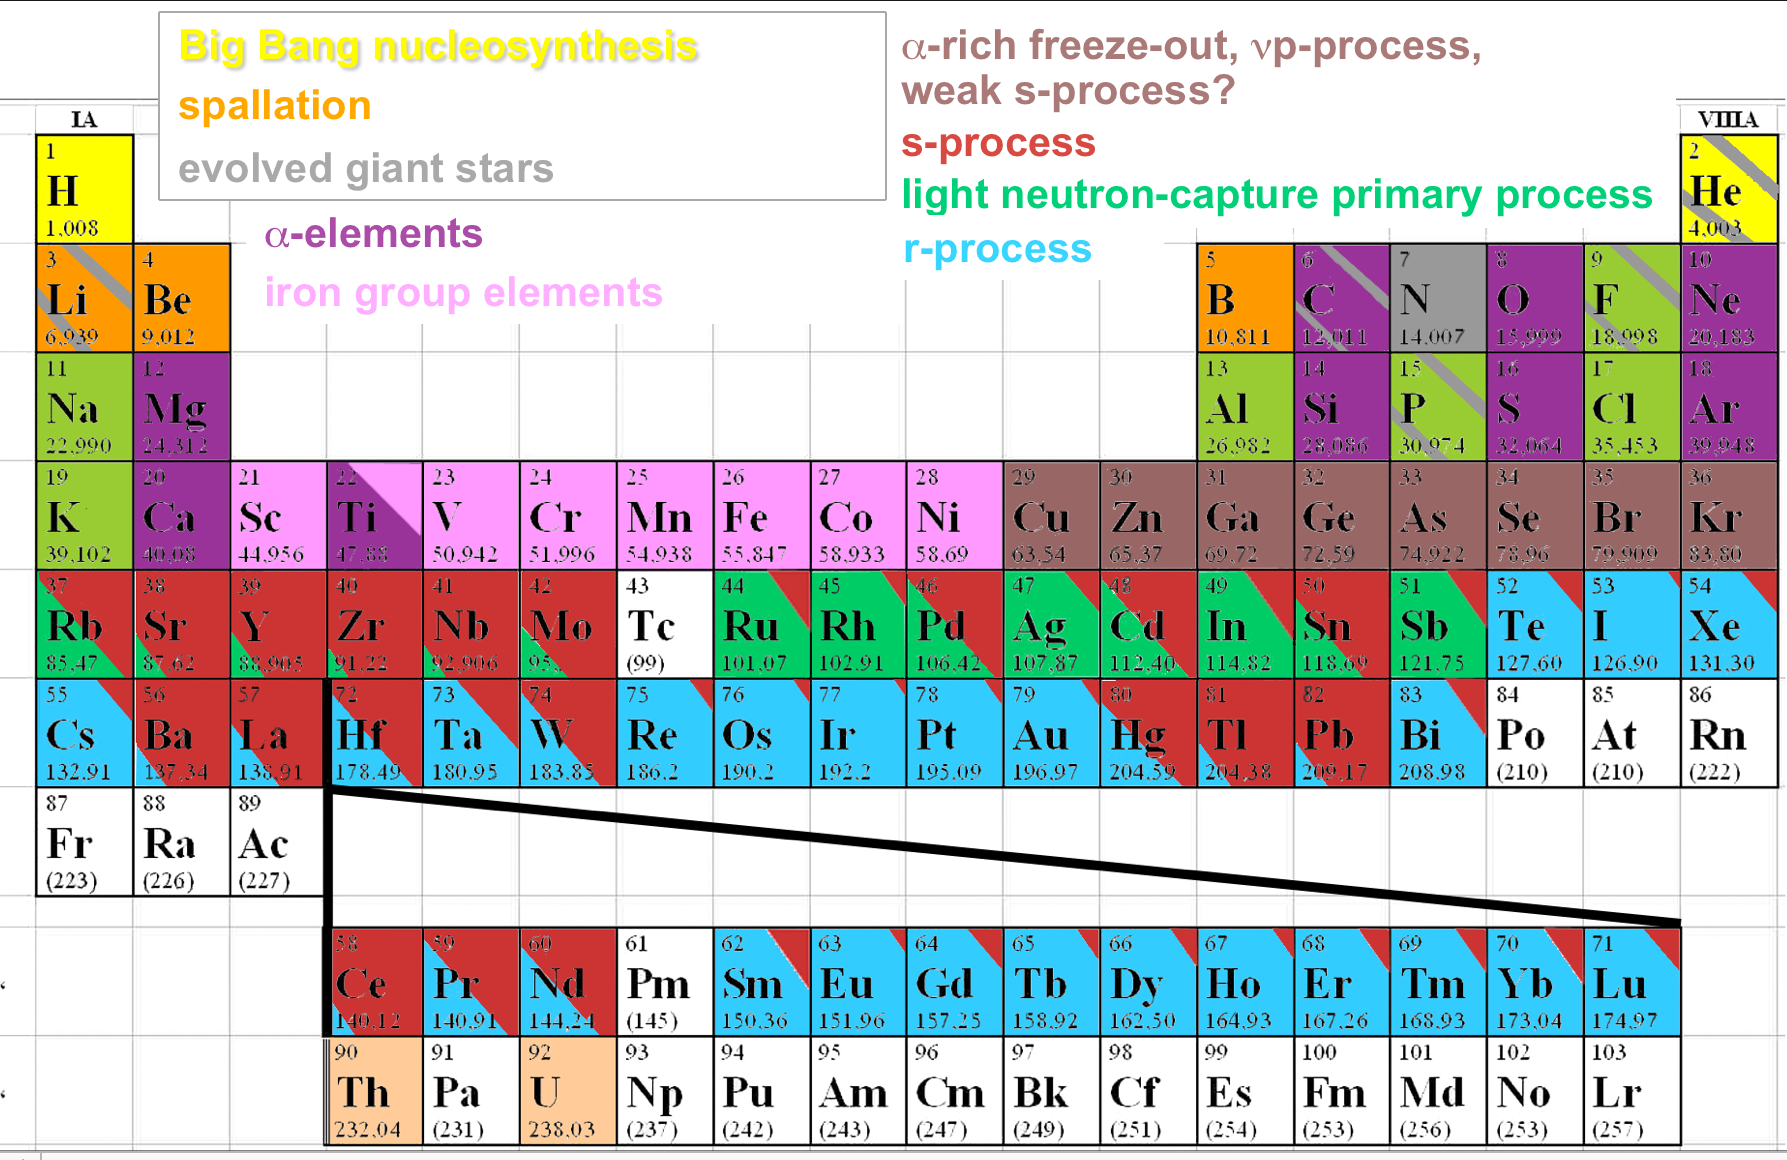
\includegraphics[width=0.75\linewidth]{./figures/intro/periodic_table}
  \caption{The periodic table of elements colored by the relative fraction of the nucleosynthetic processes that naturally occur in the Universe that produce each element. \textbf{Image Credit:} A modified version of the table created by Anna Frebel (\url{https://www.dropbox.com/sh/ib3agt2bkxqqk2u/AACbEw1warp74qzUh2AcWqfja?dl=0}), accessed on 03-18-19.}
  \label{intro:fig:periodic table}
\end{figure}

A variety of nucleosynthetic processes occur within stars and during their deaths that lead to the production of all of the elements in the periodic table. This is illustrated well in Figure~\ref{intro:fig:periodic table}, which shows the periodic table colored by the fractional importance of the nucleosynthetic processes that produce each element. Due to the diversity in production sources across the periodic table, multi-element metal abundance measurements in stars can be used to to better understand and constrain how and where each metal is produced. Exactly which reactions occur where depend strongly on the initial abundances of elements in stars, their stellar masses, and, for heavy nuclei, the neutron density.

This means that elements from different nucleosynthetic channels are produced on different timescales during a galaxy's evolution, as set by the lifetimes of the stars in which they occur, and are released into the galaxy at different energies, with different spatial distributions within the galaxy, and at different rates. For example, O, an $\alpha$-element is produced predominately in massive stars and is therefore released via core collapse supernovae on timescales of $\sim$~10~Myr after a star formation event, near their stellar birth sites. By contrast, Sr is produced predominately via the s-process (discussed more below) which occurs in part in the asymptotic giant branch (AGB) winds of lower mass stars ($M < 8$~M$_{\odot}$) at much lower energies and on timescales of $\sim 100$~Myr - $1$~Gyr. By this time, these stars would have diffused farther away from their birth sites, potentially sampling a qualitatively different portion of the ISM than the preceeding core collapse SNe. Generally, how different timescales affect observed stellar abundances patterns are well understood and easily modeled.\footnote{The canonical example of this is the ``knee" feature in a $[\alpha/$Fe] vs. [Fe/H] diagram, where the location of this knee signifies the point at which Type Ia enrichment (which produces significant Fe, but little to no $\alpha$ elements) begins to have a significant contribution over core collapse SNe (rich in $\alpha$ elements, but not Fe) \citep[e.g.[]{MatteucciBrocato1990, Geisler2005, Hill2018}. The location of this knee in this diagram shifts for a given galaxy depending on its SFH.} However, it is not well understood how differences in where and with what energies these events occur affect observed stellar abundance patterns. Investigating these differences is a key motivation of this \dissertation.

As relevant to this work, we briefly summarize a few of the important nucleosynthetic channels shown in Figure~\ref{intro:fig:periodic table} and their sites. $\alpha$-elements, notably O, Mg, Si, Ca, and Ti, are produced during the lifetime of massive stars (O, Mg) or during the core collapse supernova explosion itself. In either case, these elements are synthesized through the capture of an $\alpha$ nucleus, progressing towards increasingly heavier nuclei in intervals of 4/2 in mass/atomic number (as $\alpha$ = $^{4}_2$He) from $^8_4$Be all the way to the stable $^{52}_{26}$Fe and unstable $^{56}_{28}$Ni (which days to $^{56}_{26}$Fe). The iron group elements, notably Fe, Mn, Co, and Ni, are produced predominately in Type Ia supernovae, with variations depending on a single vs. double degenerate scenario, the initial composition of exploding white dwarf(s) (WD), and the dynamics of the explosion itself.

The presence of these heavier elements in stars enables the formation of even heavier nuclei through neutron capture. This is categorized into two processes, the slow (or s-) and rapid (or r-) process. In the former, neutron densities are typically low enough that the product of each neutron capture beta decays to a more stable isotope before capturing another nucleon. In r-process, however, the rate of neutron capture exceeds beta decay, allowing for the production of different, typically heavier, nuclei. As shown in the diagram, lighter elements are produced via the s-process and heavier via the r-process, with notable overlap in certain elements, such as Ba.\footnote{For the sake of this discussion, the light neutron-capture primary process elements (sometimes referred to as ``lighter element primary process") should be considered s-process elements. Briefly, this different nucleosynthetic channel, first identified in \cite{Travaglio2004}, arose from the disagreement between models of s-process enrichment and stellar abundances of elements including Sr, Y, and Zr. However there is still uncertainty as to whether or not these differences can be explained with different models of weak s-process (which can occur in the winds of massive stars) \citep[e.g.][]{Prantzos2018}.} The s-process occurs predominately in the low-energy winds of low mass (1-8 M$_{\odot}$) AGB stars on time scales of 100's of Myr up to 1 Gyr. Exactly which elements are produced in a given AGB star varies with stellar mass and depends strongly on metallicity, which determines the available heavy seed nuclei. Sr, Y, Zr, and Ba, as well as C, N and F, are commonly used as observational tracers of this nucleosynthetic channel.

The dominant origin of r-process enrichment is highly uncertain, though possible channels include NS-NS and neutron star - black hole mergers, neutrino driven winds in core collapse SNe, and exotic SNe, such as magnetic, jet-driven SNe, collapsars, hypernovae, and long-duration gamma-ray bursts \citep[see ][ for recent reviews]{Frebel2018, Cowan2019}. Eu is the most commonly used (and easy to observe) unambiguous observational tracer of r-process enrichment; Ba is also often studied as a tracer, but requires care due to the significant contribution from s-process enrichment. More detailed spectra \citep[e.g.][]{Ji2018a} can trace many more of these elements, which can be used as an important discriminator between nucleosynthetic models.

Finally, although the production of elements unaffected by the r-process are comparatively well understood, there are still large uncertainties in both nuclear reaction rates and stellar evolution properties that affect the computed yields for any given element. As including self-consistent nuclear reactions in the interior of stars is nearly computationally impossible in galaxy-scale simulations, metal yields are generally included as averaged over an entire stellar population (see Section\ref{intro:sec:stars}) as obtained from a tabulated set of yields. These yields for a given star in a simulation are typically IMF-averaged, and occasionally mass and metallicity dependent depending on the level of detail desired in the simulation. Often, only the global metallicity is tracked in simulations, but tracking individual metal species (especially C, O, and Si which can affect the chemistry and cooling physics in the ISM) is becoming more common. The uncertainties across tabulated yields, however, mean there are often significant variations and inconsistencies between tables produced by separate groups. These can sometimes make interpreting the results of galactic chemical evolution models challenging.

\subsection{Radiative Processes and Chemistry}
\label{intro:sec:cooling}

Radiative processes are of fundamental importance in properly modeling the diversity of density, temperature, and ionization states in a multi-phase ISM. It is via radiative cooling that gas, heated by gravitational accretion onto dark matter halos, can cool, condense, become self-gravitating, and (eventually) collapse to form stars. Conversely heating, via radiative absorption or scatterings, from stellar sources within galaxies and the extragalactic sources that comprises the cosmic UV background (UVB, e.g. \cite{HM2001,HM2012,FG2011}). Tied to both of these processes is the actual chemistry that occurs in the ISM, from the primordial chemical reactions between H, He, and free electrons to substantially more complicated reactions that occur once significant amounts of metals are present in the ISM (particularly, C, O, and Si). These metals by themselves act as additional radiative coolants, which strongly dictate the shape of the cooling curve that helps establish a multi-phase medium in the first place \citep[e.g.][]{McKeeOstriker1977}. The molecules produced in chemical reactions with these metals produce additional coolants in the ISM \citep{HollenbachMcKee1979}, including dust, which has its own rich array of associated physical processes \citep{Omukai2000,Omukai2005,Draine2011}.

A full, detailed model of radiative cooling, heating, non-equillibrium chemistry, and dust is generally far too computationally expensive to include in galaxy-scale simulations. For this reason, many large-scale cosmological simulations assume that all gas is optically thin and that all molecules and ionization states exist in equilibrium. This allows for the quick use of tabulated look-up tables for radiative cooling and heating, often produced using \code{cloudy} \citep{Cloudy2013}, that depend on gas density, temperature, metallicity, and redshift (which sets the UVB heating rate). More complex simulations often track some number (usually $< 10$) of species involved in primordial chemistry in order to better account for non-equilibrium effects and \Hmolecular production, though with noted increases in memory requirements and computational cost. Some of the most advance models to-date can account for well over 10$^2$ individual chemical reactions involving $>$ 20 elements and molecules \citep[e.g.][]{Richings2016,Richings2018}; but these are typically prohibitively expensive to run on large scales. In this \dissertation we adopt the chemistry and radiative cooling and heating physics models available in the newly developed, open-source library \code{GRACKLE} \citep{GrackleMethod}. The exact physics included in our simulations are discussed in greater detail in Chapter~\ref{ch:chapter1}, but we note that improvements to \code{GRACKLE} have been made as the direct result of the research conducted during this \dissertation.
%mention that I made improvements to this?

\subsection{Star Formation} \label{intro:sec:sf}

In galaxy-scale hydrodynamics, the costs in resolving the spatial scales and gas densities required to directly follow star formation relegates this process to a sub-grid model. Stars form from fluid elements that surpass a variety of threshold conditions at an assumed rate and efficiency. Usually, simulators set these thresholds to fully encompass gas whose Jeans-length (and thus dynamical behavior) becomes unresolved according to the widely-used \cite{Truelove1997} criterion. Often, gas is required to surpass a simple mass or number density threshold, on top of which simulators can also require that the local gas cells be in a converging flow ($\nabla \cdot \bm{v} < 0$), that gas surpass some virial threshold (describing how bound a cloud may be)
%cite?,
or that gas meet a minimum \Hmolecular mass fraction \citep[e.g.][]{Kuhlen2012}
%\citep[e.g.][]{}
. Once a fluid element is flagged as star forming, simulators have a few options to choose from in how to determine what fraction and with what rate that mass is converted into stars. Briefly, some form of the following equation is usually adopted to describe the star formation rate density,
\begin{equation}
\label{intro:eq:sfr}
 \dot{\rho}_{\rm SF} = \epsilon \frac{\rho_{\rm gas}}{t_*},
\end{equation}
where $\rho_{\rm gas}$ is the local gas density, $\epsilon$ is some fixed or variable star formation efficiency, and the timescale, $t_*$, is often adopted as the local free fall time, or
\begin{equation}
  t_* = t_{\rm ff} = \sqrt{\frac{3\pi}{32 \rm{G} \rho_{\rm gas}}}.
\end{equation}
In many cases, $\epsilon$ is fixed to some small value ($\sim$ 0.01) \citep{KrumholzTan2007} meant to represent a galaxy-scale average of star formation efficiency, even though this may vary significantly between individual molecular clouds \citep{Grudic2018}. High-resolution simulations, where the mass of stars that would form in a single time step ($dt \times \rm{SFR}$) is far less than a single star particle mass, allow stars to form out of star forming fluid elements stochastically \citep[e.g.][]{Goldbaum2015}.

Recent work has demonstrated that variations in these implementations can lead to dramatic differences in the outcome of the simulated galaxies \citep[e.g.][]{Hopkins2013,Munshi2018}. However, it is generally found that the differences between implementations decrease in simulations with sufficient resolution ($\sim$ 10~pc or better spatial, or $\sim$ $100$ M$_{\odot}$ or better in mass) and with a sufficiently high density threshold for star formation ($n > 100$~cm$^{-3}$) \citep{Orr2018,FIRE2}.

% maybe a section on each FB method? R

\subsection{Stars in Simulations} \label{intro:sec:stars}

Stars, particularly in large-scale cosmological simulations, are commonly represented as simple stellar populations (SSPs), or particles with IMF-averaged properties of stellar feedback and metal enrichment. As demonstrated in \cite{Revaz2016}, this approach is reasonable so long as the mass of the star particle is large enough to fully sample the IMF ($> 10^{4}$~M$_{\odot}$). In high resolution simulations, particularly simulations of small, low-mass systems like dwarf galaxies, this is no longer the case. This leads to inconsistencies in both the effective metal yield of the modeled stars, and (often) an artificial reduction of the effects of stellar feedback. Recent works have developed new models to address this issue, discretizing (rather than averaging over) individual feedback events \citep[e.g.][]{MUGS2010,FIRE,Hopkins2018,Rosdahl2018} or accounting for stochastic sampling of the IMF \citep{Hu2016,Hu2017,Applebaum2018,Su2018}. However, each of these methods utilizes a sub-grid recipe in some fashion to improve upon the SSPs. On the other extreme are highly resolved simulations which model star formation with ``sink particles" \citep[see for example ][]{Krumholz2004,Federrath2010,GongOstriker2013,BleulerTeyssier2014,Sormani2017} that account for the gradual accretion of gas in the growth of a single star (or group of stars) and protostellar feedback. These recipes are often computationally expensive, however, restricting their use over long timescales (100's to 1000's of Myr or more) in galaxy-scale simulations.

In this \dissertation, we develop the first implementation that breaks the SSP formalism entirely by following stars as individual star particles sampled from an adopted IMF. This allows us to place unprecedented detail on both the stellar feedback and metal yields associated with each star, spatially and temporally resolving differences in both of these channels as a function of stellar mass and metallicity.

\subsection{Stellar Feedback} \label{intro:sec:feedback}

The first models of galactic evolution produced galaxies with stellar masses far in excess of what is observed in the Universe.
%, converting a substantial fraction of their baryons into stars.
From these initial works, it was clear that some form of feedback process must take place to self-regulate star formation within galaxies. With observations of metal abundances in the CGM around galaxies \citep[see][ for a recent review]{Tumlinson2017}, and of fast-moving outflows from star forming galaxies \citep[see][ for a review]{Veilleux2005}, it was additionally clear that some mechanism must exist to drive these outflows. Stellar feedback became the clear physical mechanism to account for both of these phenomena.\footnote{Except maybe for more massive galaxies, where active galactic nuclei may play some role in regulating star formation and certainly play a role in driving outflows \citep[e.g.][]{Fabian2012}. We do not discuss this source of feedback further in this \dissertation aside from noting that it is another significant uncertainty in our understanding of galactic evolution.}

Initial models for stellar feedback relied primarily on the energy injection from supernovae (SNe, see Section~\ref{intro:sec:supernovae}) to regulate star formation and drive outflows, but it has become clear that this mechanism alone cannot completely account for all of the star formation, ISM, outflow, CGM, and even intergalactic medium (IGM) properties of observed galaxies (see \cite{SomervilleDave2015} and \cite{NaabOstriker2017} for recent reviews and more detailed discussion of how feedback impacts outstanding problems in galactic evolution). Other sources of effective stellar feedback have been identified since \citep[e.g.][]{Agertz2013}, which serve to regulate star formation on different timescales and help develop and ISM and CGM with different phase and ionization properties. This includes both stellar radiation (Section~\ref{intro:sec:radiation}) and stellar winds (Section~\ref{intro:sec:stellarwinds}).

Although not included in this \dissertation, for the sake of completeness, we mention a few additional sources of stellar feedback that likely contribute to the full picture of galactic evolution. A substantial amount of recent research has been dedicated towards the examination of supernova-driven cosmic ray feedback (see Section~\ref{ch1:sec:CRs} for a more detailed discussion and references). In brief, cosmic rays can be a dominant source of heating in very dense gas and act as a source of non-thermal pressure in the ISM, which can drive galactic winds with qualitatively different phase structures \citep[e.g.][]{SalemBryanCorlies}. Binarity is often ignored in models of stellar feedback. The effects of binary evolution can dramatically extend the timescales over which ionizing radiation and supernovae act in a newly formed stellar populations. Typically, this increases their total energy output and decreases the ISM densities in which SNe explode, increasing their effectiveness (see Section~\ref{ch1:sec:binary stars}). Finally, exotic sources of stellar feedback, such as hypernovae, high-mass X-ray binaries, and NS-NS mergers can also be a potentially important sources of feedback, particularly in the lowest mass halos \citep[e.g.][]{Artale2015}. However, the uncertainties in the frequency and delay time distributions for when these events should occur, and their relative rarity, preclude including these effects in this \dissertation.

\subsubsection{Supernova Feedback}
\label{intro:sec:supernovae}

In the simplest model, supernova feedback is treated as the injection of pure thermal energy (and mass) into the fluid element(s) that are host / closest to the chosen site of a supernova explosion. In self-consistent models of star formation and feedback these sites are usually actual star particles, but this does not have to be the case. The first models which included supernova feedback lacked the spatial / mass resolution to resolve individual (or even collective) SN events. This is the source of the commonly known ``overcooling" problem, whereby too little energy is injected into too much mass such that the affected region only reaches modest temperatures ($T \lesssim 10^5$~K, as opposed to $T > 10^7$~K, or so). This temperature is right around the peak of the cooling curve, and thus the energy is rapidly radiated away before it has time to make a significant dynamical impact of the galaxy. This is still a problem today in large-box simulations of cosmological volumes which have insufficient resolution to resolve individual SNe. While some of the initial, ad-hoc fixes for this problem (e.g. turning off cooling for some time in SN affected fluid elements or decoupling SN affected SPH particles from the hydrodynamics for some time) are still in use today, some notable advancements have been made to employ some combination of kinetic, momentum, and thermal energy feedback to attempt to capture SNe in a more consistent fashion \citep[e.g.][]{FIRE,Simpson2015,Hopkins2018}.

High resolution simulations, like those developed in this \dissertation, can typically rely on using pure thermal energy injection while still avoiding artificial overcooling.\footnote{This is advantageous because it is often substantially easier to implement than kinetic / momentum injection methods while being less susceptible to numerical artifacts, especially for grid-based codes.} This is true for simulations with typical spatial / mass resolutions better than a few pc / 10 M$_{\odot}$ \citep{Simpson2015,Hu2018,Smith2018b}. However, a spatial resolution requirement is a density dependent statement; in this case supernovae that occur in the densest gas ($n > 10^{2-3}$~cm$^{-3}$) may still be under-resolved and ineffective. In this case, accounting for feedback processes from massive stars that occur before the first core collapse SN in a given star formation event becomes critical \citep{Hu2016}. Including these physics, as discussed below, greatly reduces the typical ISM densities in which SNe occur, greatly increasing the likelihood that these events are well resolved.

\subsubsection{Stellar Radiation}
\label{intro:sec:radiation}

We only briefly discuss this method of feedback here, as it is discussed in much more detail in both Chapters~\ref{ch:chapter1} and \ref{ch:chapter2}. In brief, \cite{Leitherer1999}, \cite{Agertz2013}, and others have demonstrated that stellar radiation accounts for a substantial fraction of the total energy output of a stellar population. Ionizing photons from young, massive stars can photoionize and heat the gas surrounding sites of recent star formation. This pre-processes the local environment within which SNe occur, often increasing the effectiveness of SNe in regulating star formation and driving outflows \citep{Hu2016}. In addition, radiation pressure in the single-scattering limit (from UV photons) and rescattered infrared photons has been used as an additional source of pre-SN feedback \citep[e.g.][]{FIRE}. However, due in part to differences in how ionizing radiation is followed across simulations, there is disagreement as to exactly how and in what conditions this acts as a source of feedback (see \cite{Krumholz2018} for a detailed examination of this problem).

Non-ionizing radiation also contributes to the regulation of star formation and the multi-phase ISM. Far ultraviolet (FUV) photons contribute to gas heating via the photoelectric heating of dust grains. This is a significant heating mechanism in higher metallicity environments, like the Milky Way \citep{Parravano2003,Wolfire2003}, but may still be important in setting temperature floor of cold dense gas in lower mass galaxies \citep{Forbes2016,Hu2017}. Lyman-Werner (LW) band radiation regulates the \Hmolecular~ abundance, which is particularly important in low-metallicity environments where \Hmolecular~ is a dominant coolant \citep[e.g.][]{Glover2003,Wolcott-Green2012}.\footnote{And is arguably even more important when using star formation perscriptions that depend upon the local \Hmolecular mass fraction.} As the goal of this \dissertation is to develop an as-complete-as-possible model of galactic chemical evolution, we account for each of these processes in some fashion.

The simplest way to model stellar radiation feedback is to apply an optically thin, analytic radiation profile, such as the galaxy-centered exponential photoelectric heating profile used in \cite{Tasker2009}, or $1/r^2$ profiles from individual sources \citep[e.g.][]{Forbes2016}. However, radiative transfer effects, such as gas self-shielding, are often important, particularly for ionizing radiation. Solving the equations of radiative transfer directly in simulations -- as is done with ray tracing methods -- is computationally expensive and scales significantly with the number of sources. For this reason, approximate methods, such as flux-limited diffusion, treat radiation as a fluid, removing the scaling of computational cost with the number of sources. In this \dissertation, we follow the evolution of galaxies that have at most $10 - 100$ ionizing sources at one time, making it computationally feasible to use the accurate adaptive ray-tracing radiative transfer method implemented in \code{Enzo}.

\subsubsection{Stellar Winds}
\label{intro:sec:stellarwinds}

Stellar winds, in addition to stellar radiation, are a potentially important source of pre-SN feedback that helps regulate star formation in / around the birth clouds of newly formed stars. However, the hot ($T>10^{6}$~K), fast ($v \sim 10^{3}$~km~s$^{-1}$) winds from massive stars \citep{Weaver1977} are challenging to model self-consistently in galaxy-scale simulations. For this reason, there has been comparatively little research on how they affect global galaxy properties, even though some models do include their energy injection in an integrated / approximate fashion \citep[e.g.][]{FIRE}. However, stellar winds, from both massive stars and weaker winds from the AGB phase of low mass stars, are important sources of metal enrichment. For this reason we include stellar wind feedback in this \dissertation, albeit in a simplified fashion.\footnote{Although we do not have conclusive results to this end, initial examination of our simulations has shown that our stellar wind model is only globally important in simulations where radiation feedback is ignored. It is thus likely sub-dominant to radiation feedback.}

\section{Observations of Local Group Dwarf Galaxies}
\label{intro:sec:LG dwarfs}

We are motivated by using a properly formed model for galactic chemical evolution in dwarf galaxies to interpret and explain observations of Local Group dwarfs. As any good theoretical work should maintain a close connection to the observations that motivate the study in the first place in order to better make predictions for future observations, we devote some time here to summarize relevant observations of Local Group dwarfs.

\subsection{Known Dwarf Galaxies of the Local Group}
\label{intro:sec:dwarf galaxies}

The Milky Way and its local environment is host to a diverse collection of dwarf galaxies. The properties of these galaxies have been nicely summarized in a recent review \citep{Tolstoy2009}, and again in \cite{McConnachie2012}. However, the number of known Local Group dwarf galaxies has increased dramatically since that time, particularly for the Milky Way, whose known satellite population has more than doubled. This is due in large part to tremendous improvements in our ability to detect galaxies on the faintest end of the luminosity function, called ultrafaint dwarf galaxies \citep[UFDs][]{Willman2005}.\footnote{See \cite{Simon2019} for a recent review}. The Dark Energy Survey \citep[e.g.][]{Drlica-Wagner2015} and Hyper Supbrime-Cam \citep[e.g.][]{Greco2018} have made tremendous advances to this end, with the upcoming Large Synoptic Survey Telescope expected to produce an even greater increase in the known population of faint galaxies in the Local Group \citep{Haynes2019,Weisz2019}.

While there is no true sharp transition below which a galaxy is considered ``dwarf", historical definitions are based on luminosity cuts, using the SMC and LMC as rough anchor points for the upper-end of the dwarf galaxy scale. \cite{Bullock2017} suggests a delineation based on stellar mass. For this \dissertation, we follow this definition and consider galaxies with $M_* < 10^9$~M$_{\odot}$ as dwarf galaxies, and galaxies with $M_* < 10^5$~M$_{\odot}$ as UFDs. In general, dwarf galaxies are extremely dark matter dominated, with mass to light ratios over 10$^2$ \citep{SimonGeha2007,Strigari2008,Wolf2010}, convert gas into stars at a lower efficiency than more massive galaxies (cite), and, for the lowest mass dwarf galaxies
% need citations
, exhibit bursty star formation histories driven by stochasticity in the process of both star formation and the effects of stellar feedback
% need citations
.

\subsection{Metals in Local Group Dwarfs}
\label{intro:sec:metals in LG}

The first studies of stellar abundances in the Local Group focused on stars in nearby dwarf spheroidals (dSph's), and massive stars in the LMC, SMC, and similar, more massive dwarf galaxies. These studies typically obtained abundances for only a small sample ($\sim$ 10) stars, limiting the extent to which they can be used to test models of galactic chemical evolution.  However, the advent of high-resolution spectrographs at both Keck and the Very Large Telescope -- capable of obtaining the spectra of many stars with a single pointing -- have dramatically increased the sample size of stellar abundances in nearby dwarf galaxies.

Stellar feedback drives outflows, galactic winds, from galaxies across all scales
%(references).
Dwarf galaxies in particular, with their relatively shallow potential wells, are expected to drive effective galactic winds \citep{MacLowFerrara1999} with mass loading factors ($\eta$ = $\dot{\rm{M}}_{\rm out} / {\rm SFR}$) above 100 \citep{Muratov2015,Christensen2018}. Not only does this correspond to a significant amount of mass outflow from these galaxies, but these winds should also carry out a substantial amount of metals from these galaxies. In fact, the differences with which different models for feedback-driven winds drive metals in outflows in low mass galaxies can be an important constrain on the underlying physics \citep[e.g.]{Wheeler2018,Agertz2019}. \cite{Kirby2011-metals} used measurements of the stellar abundances in Local Group dSph's and their resolved star formation histories to determine that their stars contain less than 5\% of the metals synthesized in each galaxy. However, since these galaxies have lost their gas through environmental processes as satellites of the Milky Way (primarily ram pressure and tidal stripping), it was unclear if this loss could be attributed entirely to feedback. However, using gas and stellar abundances \cite{McQuinn2015} showed that Leo P -- a gas-rich Local Group dwarf galaxy -- has also ejected $\sim$95\% of its metals (see Section~\ref{intro:sec:Leo P}). This is significant evidence for metal-enriched, feedback-driven galactic winds operating in these low mass dwarf galaxies.

Finally, the low metallicities of the lowest mass dwarf galaxies make them ideal places to better constrain large uncertainties in stellar nucleosynthesis \citep{FrebelNorris2015,Frebel2018}. At these low metallicities, the number of possible enrichment events that could have possibly contributed to the observed stellar abundances decreases significantly, increasing the possibility of using these abundance patterns to constrain the yields of individual sources. This is particularly true for exotic enrichment events, like those expected to be sources of r-process elements, which are potentially so rare that only one or fewer events would be expected in an individual low-mass galaxy.

The most prominent example of these types of studies has been of the UFD Reticulum II, where \cite{Ji2016} used the extreme r-process enhancement in its stars to argue in favor of a NS-NS of r-process enrichment. This conclusion has been supported by observations in additional Local Group dwarf galaxies \citep{Duggan2018}, but there is still some disagreement as to the dominant source of r-process enrichment \citep[e.g.][]{Siegel2018}. Interestingly, the lack of these extreme r-process abundances in other UFDs suggests that another source of r-process must exist \citep{Ji2016b}. Some of the significant uncertainties in interpreting these observations lie with understanding how r-process elements mix within the ISM and are ejected from low mass dwarf galaxies. Recent research has examined how metals from individual enrichment events may mix and evolve in a variety of contexts \citep[e.g.][]{Bland-Hawthorn2015,Ritter2015,Montes2016,Safarzadeh2017}, but there is still much to be understood about this process. In particular, there is still much to be gained from adapting insights from these types of simulations to the modeling used to interpret observations of stellar abundances (as discussed in more detail in Section~\ref{intro:sec:onezone}).

\subsection{Leo P: A Case Study}
\label{intro:sec:Leo P}

\begin{figure}
 \centering
 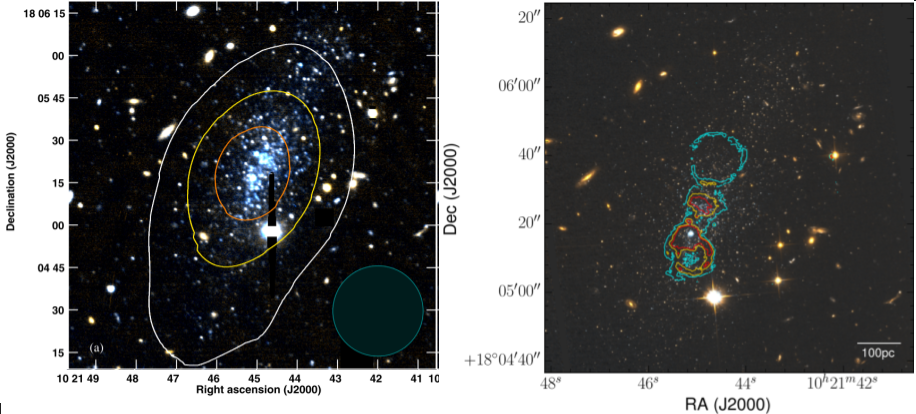
\includegraphics[width=0.975\linewidth]{figures/intro/Leo_P}
 \caption{The Leo P dwarf galaxy. \textbf{Left:} \hi contours from the Very Large Array (VLA) at 32'' resolution overlaid on top of an optical Large Binocular Telescope image. 32'' is the lowest resolution \hi observation available of Leo P from the VLA, which best traces diffuse, warm ($T \sim 10^3$~K) \hi in the galaxy and exhibits the full spatial extent of its gas content. This image is adopted from the top-left panel of Figure 4 in \cite{Bernstein-Cooper2014}. \textbf{Right:} H$\alpha$ emission (contours) overlaid on top of a Hubble Space Telescope (HST) optical image. The \hii region analyzed in \cite{McQuinn2015} to obtain gas-phase metallicities is the blue clump of H$\alpha$ towards the bottom of the image. This image is adopted from Figure 10 of \cite{Evans2019}. Note the inversion in the vertical axes between the left and right panels.}
 \label{intro:fig:Leo P}
\end{figure}

We dedicate this section to a specific Local Group dwarf galaxy, Leo P, as its observed properties motivate the initial conditions of the simulations developed in this \dissertation. This galaxy is remarkable for being one of the lowest mass dwarf galaxies with observed, ongoing star formation. It is located at a distance of $1.62\pm 0.15$~Mpc \citep{McQuinn2015a}, and was first characterized as part of the ALFALFA survey \citep{Giovanelli2013,Rhode2013,Skillman2013,McQuinn2013,Bernstein-Cooper2014}. These studies have characterized its star formation history as low and roughly continuous over the age of the Universe \citep[$<$SFR$>$ = $4.3\times 10^{-5}$~M$_{\odot}$~yr$^{-1}$,][]{McQuinn2015a}, its stellar mass \citep[$M_{*} = 5.7 \times 10^{5}$~M$_{\odot}$,][]{McQuinn2013}, its \hi and dynamical mass \citep[$M_{\rm HI}(r<r_{\rm HI}) = 9.5\times 10^{5}$~M$_{\odot}$, $M_{\rm dyn}(r<r_{\rm HI}) = 2.6 \times 10^{7}$~M$_{\odot}$, $r_{\rm HI} \sim 500$~pc,][]{Bernstein-Cooper2014}, and gas-phase abundances from an \hii region \citep[12 + log(O/H) = 7.17$\pm$0.04][]{Skillman2013}. HI, optical, and H$\alpha$ observations of Leo P are shown inf Figure~\ref{intro:fig:Leo P}.

We chose to focus on a Leo P like galaxy in our simulations in part to allow for comparisons to the work in \cite{McQuinn2015}, which makes an accounting of the total metals (as traced by O) contained in the ISM and stars in Leo P, estimating the fraction that must have been ejected over the lifetime of the galaxy.
%This is an important measurement as prior estimates of this number for low mass dwarf galaxies were restricted to Milky Way dSph's, which are devoid of gas and contaminated by environmental affects.
As of this writing, Leo P is one of the only low mass dwarf galaxies with both gas-phase and stellar metal abundance measurements, but there is ongoing work to greatly expand this sample in the near future.

\section{Onezone Models of Galactic Chemical Evolution}
\label{intro:sec:onezone}

This \dissertation utilizes high-resolution hydrodynamics simulations that are expensive to run in terms of both wall-time ($\sim$ weeks to months) and computational time ($\sim 10^{5-6}$ CPU hours). For this reason, it is computationally infeasible to directly explore many of the uncertainties associated with each of the components of the model as discussed in Section~\ref{intro:sec:ingredients}. For this reason, substantially cheaper semi-analytic models are valuable tools that can be used to better understand galactic evolution.

One of the most common ways to model and understand the stellar populations of galaxies in high-dimensional chemical space is through simplified one-zone (or many-zone) models. This treatment extends back many decades \citep[e.g.][]{Schmidt1963,TalbotArnett1971,Lynden-Bell1975}, where galaxies and their total metal abundances were treated in closed-box systems of gas and stars. Over the intervening decades these models have improved, including prescriptions for gas outflow (a ``leaky-box") or gas inflow (an ``accreting box"), or both \citep[a ``bathtub" model, e.g.][]{FinlatorDave2008,Bouche2010}. The assumptions that go into these models vary dramatically with complexity. Simple models can assume, for example, that long-lived low mass stars do not contribute to metal enrichment while metals from massive stars are instantaneously recycled into the galaxy's gas reservoir (i.e. ignoring stellar lifetimes) or that all metals mix instantly and homogeneously. More complex models account for individual stellar lifetimes (to some degree), or may try and account for some aspects of inhomogeneous mixing by constructing multi-zone models that may separate a galaxy in radial bins (with or without mixing between bins), may account for a hot and cold component separately (with mixing between the two), or account for separate ISM and CGM components. The output of these models is typically the mean metal abundance evolution within each of the tracked components. There is generally no self-consistent prescription to account for the scatter in any abundance relationship in these models, which, when needed, is often added ad-hoc in post-processing. Regardless of the assumptions that go into these models, they are powerful tools that can be used to probe the general physical processes that govern galactic chemical evolution, and explore the vast, uncertain parameter space associated with the models that characterize these processes \citep[e.g.][]{Cote2017a}.

One final motivation of this \dissertation is to improve the assumptions within these models by better characterizing the process of inhomogeneous mixing in the ISM, and the coupling of metals to galactic winds and outflows. This is particularly important if the behavior differs between elements from different nucleosynthetic sites. In addition, this work could be used to account for the spread and higher-order statistics of stellar abundance distributions, which would be a powerful tool for better leveraging the wealth of observations in the Milky Way and Local Group. Yet, as discussed, the current state of the art prescriptions for these processes are ad-hoc. Recent analytic work in \cite{KrumholzTing2018} lays down a framework to evaluate the correlation between individual metals in different galactic environments and predicts that the correlations will differ for different nucleosynthetic sites (e.g. AGB winds vs. SNe). We characterize these differences in detail in Chapter~\ref{ch:chapter3}, laying the groundwork for how one could potentially incorporate this insight into improving these models. We build upon this idea more in Chapter~\ref{ch:chapter4}, and plan to explore the connection between our simulations and analytic models in the future. Recent work by \cite{SchonrichWeinberg2019} is a great example of how this could impact current models for galactic chemical evolution. The authors show how adopting a two-phase model (hot and cold ISM), along with parameters for how metals are injected and mix between the phases whose values differ depending on nucleosynthetic origin of the metal, can reconcile long-standing problems in understanding the r-process abundance evolution of stars in the Milky Way. In fact, they argue that it would be impossible to reproduce observed r-process abundances in the Milky Way (namely [Eu/Fe], [Eu/Si], and [Eu/Mg] as functions of [Fe/H]) with a standard one-phase model.


\section{Structure of \dissertation}\label{intro:sec:structure}
\label{intro:sec:structure}

In this work we investigate the role of both stellar feedback and mixing in a multi-phase ISM in driving galactic chemical evolution. Using a novel method for following star formation and stellar feedback in galaxy-scale hydrodynamics simulations, we provide significant insight into how individual metals from distinct nucleosynthetic sites enrich the ISM, how their abundances are set and imprinted upon newly formed stars, and how they are ejected from galaxies through galactic winds.

In Chapter \ref{ch:chapter1} \citep[published as][]{Emerick2019}, we motivate the need for a new model of star formation and stellar feedback to address the open uncertainties in galactic chemical evolution. We implement such a model, which follows stars as individual star particles over a fully sampled IMF, in hydrodynamics simulations of an isolated, low-mass dwarf galaxy. We describe in detail the physics included in these simulations, including a stellar feedback model that follows stellar radiation, stellar winds, and supernovae. We find that the implemented set of physics give rise to a multi-phase ISM with a highly variable stellar radiation profiles, star formation rates, and galactic outflows. In agreement with previous works, we find that multi-channel feedback is able to drive outflows with high mass-loading factors while maintaining a fluctuating star formation rate density consistent with observations of low mass dwarf galaxies. Finally, we characterize the \Hmolecular~ properties of this galaxy, which remains unconstrained in observations of dwarf galaxies at this mass scale.

In Chapter \ref{ch:chapter2} \citep[published as][]{Emerick2018a}, we investigate how stellar ionizing radiation feedback impacts the evolution of our simulated low mass dwarf galaxy. We confirm the findings in recent works, as discussed in Section~\ref{intro:sec:radiation}, that find that stellar radiation is an important source of pre-supernova feedback that regulates star formation and can help drive galactic outflows. We additionally investigate how radiation feedback couples to the ISM to drive galactic winds by demonstrating that the ionization of gas far from individual ionizing sources, out into the disk-halo interface of our galaxy, creates low-density channels through which supernovae can readily drive gas and metals into and beyond the galaxy's CGM. This suggests that not only is the local deposition of energy from stellar radiation important, which quickly destroys dense gas in stellar birth-sites, but also long-range effects are important to consider in a consistent model of stellar feedback.

In Chapter \ref{ch:chapter3} \citep[published as][]{Emerick2018b}, we dive in detail into the evolution of each of the 15 individual metal species that we follow in our simulation. We focus primarily on the evolution of the gas-phase abundances of these metals, and how the site of nucleosynthesis (e.g. AGB winds or SNe) drives the subsequent evolution of each species. We find that elements released in lower energy enrichment sources (e.g. AGB winds) mix less effectively in the ISM across all phases than elements released in higher energy enrichment sources (e.g. SNe). Likewise, energy differences associated with their enrichment directly impacts their ability to couple to galactic outflows. We find that elements released in AGB winds are retained at a higher fraction (by a factor of $\sim$ 4-5) than elements released in SNe.

In Chapter \ref{ch:chapter4} we discuss recent, unpublished results which build upon the work in Chapter~\ref{ch:chapter3} by investigating in more detail how energy, spatial location within the galaxy, and galaxy SFR affect the mixing and ejection of metals for individual enrichment events. With a more detailed study, we again confirm that metal mixing in the ISM and ejection in galactic winds depends upon the energy of the enrichment event, sampling event energies from AGB winds ($\sim$ erg) to hypernovae ($\sim 10^{52}$~erg).

Finally, we conclude in Chapter \ref{ch:conclusion} and briefly discuss future work as extensions of this \dissertation.

	\chapter[Simulating an Isolated Dwarf Galaxy with Multi-Channel Feedback and Chemical Yields from Individual Stars ]{Simulating an Isolated Dwarf Galaxy with Multi-Channel Feedback and Chemical Yields from Individual Stars \label{ch:chapter1}}
\let\thefootnote\relax\footnotetext{This section contains text from an article published originally as \cite{Emerick2019}}

%
% Copy paste paper here, without abstract or keywords
%
%
% Abstract left here for documenation purposes
%
%\begin{abstract}
%In order to better understand the relationship between feedback and galactic chemical evolution, we have developed a new model for stellar feedback at grid resolutions of only a few parsecs in global disk simulations, using the adaptive mesh refinement hydrodynamics code \textsc{Enzo}. For the first time in galaxy scale simulations, we simulate detailed stellar feedback from individual stars including asymptotic giant branch winds, photoelectric heating, Lyman-Werner radiation, ionizing radiation tracked through an adaptive ray-tracing radiative transfer method, and core collapse and Type Ia supernovae. We furthermore follow the star-by-star chemical yields using tracer fields for 15 metal species: C, N, O, Na, Mg, Si, S, Ca, Mn, Fe, Ni, As, Sr, Y, and Ba. We include the yields ejected in massive stellar winds, but greatly reduce the winds' velocities due to computational constraints. We describe these methods in detail in this work and present the first results from 500~Myr of evolution of an isolated dwarf galaxy with properties similar to a Local Group, low-mass dwarf galaxy. We demonstrate that our physics and feedback model is capable of producing a dwarf galaxy whose evolution is consistent with observations in both the Kennicutt-Schmidt relationship and extended Schmidt relationship. Effective feedback drives outflows with a greater metallicity than the ISM, leading to low metal retention fractions consistent with observations. Finally, we demonstrate that these simulations yield valuable information on the variation in mixing behavior of individual metal species within the multi-phase interstellar medium.
%\end{abstract}

\newcommand{\ccunit}{cm$^{-3}$}

\section{Introduction}
Detailed interstellar medium (ISM) and chemical abundance properties of galaxies are sensitive tests of the underlying physical processes that govern galaxy evolution. Examining these in more detail in galaxy scale simulations is an important and exciting new discriminator between models. There is a considerable body of work studying the chemodynamical evolution of galaxies using cosmological hydrodynamics simulations \citep[e.g.][]{OppenheimerDave2008,Wiersma2009,Shen2010,Simpson2013,Snaith2015,OWLS,EAGLE,FIRE}.
% editor asked us to reduce citation count here:{Lia2002,KawataGibson2003,Kobayashi2004,Tornatore2004,Romeo2005,OppenheimerDave2008,Wiersma2009,Shen2010,MUGS2010,ErisSimulation,Simpson2013,Brook2014,Snaith2015,Oppenheimer2016,OWLS,EAGLE,FIRE}.
These simulations, coupled with additional attention to feedback processes, have made remarkable progress in reproducing global galaxy trends such as evolution of the mass-metallicity relationship \citep[e.g.][]{Obreja2014, Ma2016, Dave2017, Torrey2017} and more detailed quantities such as metallicity distribution functions (MDFs) and the evolution of individual species abundances \citep{Marcolini2008,Revaz2009,Sawala2010,RevazJablonka2012,Jeon2017,Hirai2017} .

However, much of this work has been done with Lagrangian smoothed particle hydrodynamics schemes, with a few recent exceptions  \citep{Few2012,Simpson2013,Few2014,Vorobyov2015,Corlies2018}. In its original form, this scheme does not capture mixing between chemically inhomogeneous particles, as necessary for chemical evolution. Mixing can be modeled with sub-grid models of turbulent metal diffusion \citep[e.g.][]{Shen2010,Shen2013,Brook2014,Su2017a,Escala2018}, but there are many possible models and each is not necessarily applicable in every regime \citep[see ][]{Revaz2016}. While mixing occurs in Eulerian codes even without sub-grid models, numerical diffusion tends to result in over-mixing in simulations without sufficiently high spatial resolution. Molecular diffusion or even turbulent mixing is certainly not resolved in any galaxy-scale simulation with either method, requiring additional sub-grid models; this can be particularly important for understanding the initial pollution of otherwise pristine gas \citep[see ][ and references therein]{PanScannapiecoScalo2013,Sarmento2017}. Moreover, metal mixing efficiencies may vary species-by-species \citep[e.g.][]{Cohen2013, Roederer2014, FrebelNorris2015, Hirai2017, Cote2018, KrumholzTing2018}. Mixing behavior is tied critically to the feedback source (stellar winds, supernovae, and possibly more exotic sources) that inject metals into different phases of
the ISM with different energies and on different timescales; the observational effect of this is poorly understood, however. The variations in how different methods handle sub-grid metal injection and metal mixing schemes can lead to uncertainties in connecting models to observations and the fundamental physics that drives galaxy evolution.

Increasing physical resolution reduces reliance on sub-grid physics for mixing.  However, at high particle mass resolution ($M \lesssim 10^3$ M$_{\odot}$) standard schemes for modeling stars as simple stellar populations lose validity  \citep[as studied in detail by][]{Revaz2016}. Below 10$^4$ M$_{\odot}$, such schemes do not fully sample the initial mass function (IMF), and cannot be considered average representations of stellar populations. This is acutely problematic at low star formation rate densities with star particle masses comparable to or below the mass of the most massive individual star ($\sim 100$ M$_{\odot}$). At high star formation rate densities, an undersampled IMF in a single low mass star particle can be compensated for by having many adjacent star particles. Various approaches exist to address this issue \citep[e.g.][]{Kobayashi2000,WeidnerKroupa2004,Pflamm-AltenburgKroupa2006,RevazJablonka2012,Kroupa2013,Rosdahl2015,Su2018}, but none are without caveats \citep{Revaz2016}, save for schemes which begin to track the star-by-star information within a given particle by directly sampling the IMF at formation time \citep[e.g.][]{Hu2017}. The most straightforward solution is to remove the single stellar population formalism entirely and simply track stars as individual particles.

We introduce a new method for studying galactic chemical evolution that follows stars as individual star particles implemented in the adaptive mesh refinement code \texttt{Enzo}, designed for high resolution simulations of isolated galaxies. The relative simplicity of idealized, isolated galaxy evolution simulations allows for a focused, first-principles approach to studying multi-channel feedback mechanisms. We follow recent work using low mass dwarf galaxies as laboratories to study in detail how feedback governs galaxy evolution \citep{Forbes2016,Hu2016,Hu2017}.
%For example, \citet{Forbes2016} found that photoelectric heating can be a significant source of feedback in small galaxies. \citet{Hu2016} and \citet{Hu2017} examined the relative importance of various feedback physics in regulating ISM properties of dwarf galaxies.
Our work builds upon our current understanding of feedback and galactic chemodynamics while making three notable advances: 1) direct star-by-star modeling, 2) stellar winds from both massive and asymptotic giant branch (AGB) stars, and 3) using an adaptive ray tracing method to follow stellar ionizing radiation. We also include core collapse and Type Ia supernova feedback, photoelectric heating from stellar far ultra-violet (FUV) radiation, and Lyman-Werner dissociation from stellar radiation.

Using star-by-star modeling, we capture in more detail the stellar yields from individual stars released over their lifetime. This includes yields from massive and AGB stellar winds, and supernovae (SNe). In addition to better capturing how individual metal species enrich the ISM, this allows us to chemically tag individual stars. This ability opens an exciting new channel for testing models of galaxy evolution by leveraging current and ongoing observations probing the detailed distributions of chemical abundances of stars in the Milky Way and Local Group, such as APOGEE and APOGEE2 \citep{APOGEE2010,APOGEE}, the Gaia-ESO survey \citep{Gaia}, and GALAH \citep{GALAH}. This paper is the first in a series examining in detail the role that individual components of multi-channel stellar feedback play in galaxy dynamical and chemical evolution. In \cite{Emerick2018b} we investigate the importance of ionizing radiation in regulating star formation and driving outflows in our galaxy. In \cite{Emerick2018b} we explore how individual metal species mix within the ISM and are ejected via galactic winds.

We describe each mode of our multi-channel feedback
in detail in Section~\ref{ch1:sec:methods}, describe their implementation in an isolated dwarf galaxy simulation in Section~\ref{ch1:sec:IC}, show results from this simulation in Section~\ref{ch1:sec:results}, discuss the results in Section~\ref{ch1:sec:discussion}, and conclude in Section~\ref{ch1:sec:conclusion}. Readers who may want to only briefly skim (or skip) over the details of our included physics are advised to just read the beginning of Section~\ref{ch1:sec:methods}, which contains a complete---yet brief---summary of the included physics.

\section{Methods}
\label{ch1:sec:methods}
We produce high-resolution, galaxy-scale simulations tracking stars not as single stellar populations, but as individual stars sampled from an assumed IMF.
This allows us to follow star-by-star variations in feedback physics and stellar yields in detail. To properly model the ISM, we track non-equilibrium, primordial chemistry (including molecular hydrogen) using \texttt{Grackle} \citep{GrackleMethod}, with heating and approximate self-shielding from a metagalactic ultraviolet (UV) background. We assume collisional ionization equilibrium for all other elements and use updated \texttt{Cloudy} metal-line cooling tables consistent with our self-shielding approximation (see Appendix~\ref{appendix:cooling}). We also include an updated observationally motivated dust model for the low metallicity regimes studied here ($Z \lesssim 0.1$ Z$_{\odot}$). Each star is assigned basic properties including surface gravity, effective temperature, radius, and lifetime from tabulated stellar evolution models, which inform how the stars deposit their feedback. We directly track ionizing radiation from massive stars using an adaptive ray tracing radiative transfer method that includes the effects of radiation pressure on HI. In addition, we follow the optically thin, non-ionizing UV radiation from these stars that cause photoelectric heating and Lyman-Werner dissociation of molecular hydrogen. We track the stellar wind feedback and SNe from these stars, depositing individual metal yields from both. We include AGB wind feedback and yields for lower mass stars, and track these directly as Type Ia SN progenitors. We follow yields for 15 individual metal species (C, N, O, Na, Mg, Si, S, Ca, Mn, Fe, Ni, As, Sr, Y, and Ba), chemically tagging each star as it forms with the associated local gas abundances for each species. In addition, we track a total metal density field which is the sum of all metals, including those not directly tracked. This field is used to inform the heating/cooling physics, and determines the metallicity of each star at birth. These methods are discussed in full detail below.

\subsection{Hydrodynamics and Gravity}
\label{ch1:sec:hydro}

We use the adaptive mesh refinement hydrodynamics and N-body code \texttt{Enzo}\footnote{http://www.enzo-project.org} to simulate the chemodynamical evolution and detailed feedback physics in a set of high resolution, isolated, low-mass dwarf galaxies. \texttt{Enzo} is an open-source code that is undergoing continual, active development by many researchers across several institutions. We use a substantially modified version of the current development version of \texttt{Enzo} (version 2.X) in this work.\footnote{This version is contained in a publicly available fork of the main repository: https://bitbucket.org/aemerick/enzo-emerick. Specifically, simulations presented here were conducted at changeset 7001d99.} We solve the equations of hydrodynamics using a direct-Eulerian piecewise parabolic method \citep{ColellaWoodward1984, Bryan1995} and a two-shock approximate Riemann solver with progressive fallback to more diffusive Riemann solvers in the event that higher order methods produce negative densities or energies. We compute the total gravitational potential from gas self-gravity, stars, and a static background dark matter potential (see Section~\ref{ch1:sec:IC}). Self-gravity is computed with a multigrid Poisson solver. The collisionless star particles are evolved with an adaptive particle-mesh N-body solver at an effective force resolution of $\sim 2 \Delta x$, where $\Delta x$ is the local cell size.

We refine the mesh whenever the thermal Jeans length is no longer resolved by a minimum of 8 cells, continually refining a given region until this criterion is met or until the region reaches the maximum resolution (1.8~pc). At maximum resolution, the Jeans length can become under-resolved, leading to artificial numerical fragmentation. \citet{Truelove1997} showed that resolving the Jeans length by at least 4 cells is required to suppress this fragmentation.

We set the star formation density threshold to the value at which the Jeans length becomes resolved by only 4 cells in sub-200 K gas, or about 200 \ccunit (as discussed further in Section~\ref{ch1:sec:star formation}). Forming stars from this gas will reduce the local density, ensuring the Jeans length is resolved. However, since star formation is not instantaneous, we employ a pressure floor to support gas against artificial fragmentation and collapse. A non-thermal pressure term is added to cells once their thermal Jeans length becomes unresolved. This prevents dense, self-gravitating gas from rapidly reaching densities significantly above our resolution limit. The use of a pressure floor is common in galaxy scale simulations with limited dynamic range \citep[e.g][]{Machacek2001, 2008ApJ...680.1083R}.

Due to computational constraints we found it necessary to institute a temperature ceiling in low density, diffuse gas. These high temperatures, typically well above 10$^{7}$~K and up to 10$^{8}$~K, would place an onerous constraint on the limiting time step at high spatial resolution. At these temperatures, with typical velocities up to $\sim$10$^{3}$~km~s$^{-1}$, satisfying the Courant condition requires time steps on order of 100~yr. We institute a maximum temperature of 8$\times 10^6$~K in gas with densities between 10$^{-30}$~g~cm$^{-3}$ and 10$^{-26}$~g~cm$^{-3}$. These densities were somewhat arbitrarily chosen, but ensure that this threshold does not impact very low density gas in the halo of our dwarf galaxy or higher density gas in supernova injection regions. This threshold decreases the required run-time by factors of a few. The value of the temperature threshold was chosen to ensure the affected hot gas remained just above the high-temperature minimum of our cooling curve (see Appendix~\ref{appendix:cooling}.)

\subsection{Chemistry and Cooling Physics}
\label{ch1:sec:chemistry}

We use the chemistry and cooling library \texttt{Grackle}\footnote{https://grackle.readthedocs.io/en/grackle-3.0/} v 3.0 to follow a nine species non-equilibrium chemistry network (H, H$^+$, He, He$^+$, He$^{++}$, e$^{-}$, H$_2$, H$^{-}$, and H$_{2}$) which includes radiative heating and cooling from these species and metals.\footnote{We use a slightly modified version of the the main \texttt{Grackle} repository, available at https://bitbucket.org/aemerick/grackle-emerick at changeset c2c0faf.} \texttt{Grackle} is a freely available, open source, multi-code library, designed to interface with a wide variety of astrophysical codes. We outline specific model choices made in our simulations and refer the reader to \citet{GrackleMethod} for a detailed discussion of the code. We apply the \citet{Glover2008} three-body rate for H$_{2}$ formation and include a model for H$_2$ formation on dust, dust heating, and dust cooling following the methods in \citet{Omukai2000} and \citet{Omukai2005} as included in \texttt{Grackle}. However, we update the default dust to gas ratio scaling in \texttt{Grackle} to account for the steeper scaling in low metallicity regimes ($Z \lesssim 0.1 Z_{\odot}$), using the broken power law scalings from \citet{Remy-Ruyer2014}. For metallicities above $\sim 0.1 Z_{\odot}$, this is equivalent to the default behavior of \texttt{Grackle}, where dust content scales linearly with metallicity.

As part of the \texttt{Grackle} package, metal line cooling is modeled using pre-computed \texttt{Cloudy} \citep{Cloudy2013} \footnote{http://www.nublado.org/} tables interpolated as a function of density, temperature, and redshift, using the \citet{HM2012} UV metagalactic background. As discussed in more detail in Section~\ref{ch1:sec:diffusive heating}, we account for approximate self-shielding of H and He against this UV background. Using this prescription with metal line cooling tables computed under an optically thin assumption can lead to an order of magnitude overestimation of the cooling rate at certain densities, as discussed in \citet{Hu2017} and  Appendix~\ref{appendix:cooling}. To address this issue, we use re-computed metal line tables consistent with the self-shielding approximation.  We have made these new tables public in the main \texttt{Grackle} repository. These are discussed in greater detail in Appendix ~\ref{appendix:cooling}. Finally, we ignore the effect the stellar radiation field (see Section~\ref{ch1:sec:diffusive heating}) may have on the interpolated metal line cooling rates.

\subsection{Star Formation Algorithm}
\label{ch1:sec:star formation}
In order to resolve individual star formation events on galactic scales, we implement a stochastic star formation algorithm adopted from \citet{Goldbaum2015,Goldbaum2016}. Each cell at the maximum refinement level is capable of forming stars if it contains gas that meets the following local criteria on number density $n$, temperature $T$, cell mass $M$, and velocity $\vec{v}$: 1) $n > n_{\rm thresh}$, 2) $T < T_{\rm thresh}$, 3) $M > M_{\rm Jeans}$, and 4) $\vec{\nabla} \cdot \vec{v} < 0$, where $n_{\rm thresh}$ is a resolution dependent density threshold, $T_{\rm thresh}$ is a temperature threshold, and $M_{\rm Jeans}$ is the local thermal Jeans mass. Our fiducial values are $n_{\rm thresh} =  200 \mbox{ cm}^{-3}$ and $T_{\rm thresh}= 200$~K. We limit the fraction of a cell's gas mass that is converted into stars by requiring $M > f_{\rm thresh} M_{\rm max,*}$, where $f_{\rm thresh} = 2.0 $ and the maximum star mass $M_{\rm max,*} = 100 \mbox{ M}_{\odot}$. No star formation occurs when $M < f_{\rm thresh} M_{\rm max,*}$, ensuring that a star formation episode can not produce negative densities.

We make the common ansatz that star formation occurs by converting gas into stars in a free fall time $\tau_{\rm ff}$ with a star formation efficiency, $\epsilon_{\rm f} \simeq 0.02$ \citep{KrumholzTan2007}. At high resolution, the choice of $\epsilon_{\rm f}$ should be irrelevant \citep{Orr2018, FIRE2}, as star formation is ultimately self-regulated by feedback.

The stellar mass formed during a timestep $\Delta t$ from a region with a total gas mass $M_{\rm gas}$ is
\begin{equation}
         M_* = \epsilon_{\rm f} M_{\rm gas} \frac{\Delta t}{\tau_{\rm ff}}
\end{equation}
In practice, $\Delta t/\tau_{\rm ff} \ll 1$, and $M_*$ is smaller than the minimum star particle mass at parsec scale resolution. We therefore allow star formation to proceed stochastically, following the methods in \citet{Goldbaum2015, Goldbaum2016}, modified for variable stellar masses. In each cell that could potentially form stars, we compute the probability that 100 M$_{\odot}$ of gas will be converted into stars in that time step, and use a random number draw to determine whether or not star formation actually occurs. If it does, we randomly sample from
the adopted IMF until approximately 100 M$_{\odot}$ of stars form, keeping the last sampled particle when the total stellar mass formed exceeds 100 M$_{\odot}$. The total mass of formed star particles is subtracted from the gas mass in the star forming region to ensure mass conservation. We assume a Salpeter IMF \citep{Salpeter1955} with $\alpha = 2.35$, sampling over the range between a minimum stellar mass of 1 M$_{\odot}$ and an arbitrarily chosen maximum stellar mass of 100 M$_{\odot}$. Our lower limit on stellar masses ensures that we are able to both directly track all particles that contribute in some way to feedback and metal enrichment, and follow longer lived star particles, while reducing the computational expense of following a large number of low mass stars that have no dynamical impact on the galaxy evolution. By ignoring the formation of stars below 1~M$_{\odot}$, our model in effect spreads this mass into higher mass stars, changing the normalization of the IMF slightly from what would be expected for an IMF that extends below  1~M$_{\odot}$.

Formed stars are deposited with random positions within the star forming cell and assigned velocities equal to the cell bulk velocity with a 1~km~s$^{-1}$ velocity dispersion. This dispersion captures some of the unresolved gas motions below the resolution limit that are smoothed out by numerical diffusion; it is comparable to, but less than, the velocity dispersion of the coldest gas in our simulations. Stars are assigned metallicities corresponding to the metallicity of the star forming zone, and are chemically tagged with the 17 individual species abundances (H, He, and the 15 metals) that we follow in our simulations.

Stars evolve during the simulation, by losing mass from stellar winds and SNe as described below, and by changing types, but persist throughout the entire simulation. For example, low mass stars are tagged as white dwarfs (WDs) at the end of their life, which may eventually explode as a Type Ia SN (discussed below), after which they persist as massless tracer particle remnants. Finally, each star is marked as a ``must refine'' particle, requiring that it be surrounded by a four-cell region at the highest level of refinement. This ensures that both stellar winds and SNe feedback are maximally resolved, and that any ejected yields are deposited over a consistent physical scale throughout the simulation.

\subsection{Stellar Properties}
\label{ch1:sec:properties}
Given each star's birth mass and metallicity, we interpolate over the PARSEC grid of stellar evolution tracks \citep{Bressan2012} to assign a lifetime and AGB phase start time (if any) to it, as well as the effective temperature $T_{\rm eff}$ and surface gravity $g$ used in computing radiation properties (see Section \ref{ch1:sec:ionizing radiation}). We use the largest subset of the PARSEC models that are regularly sampled in our mass/metallicity space of interest, with 26 mass bins over M$_{*} \in \left[0.95, 120.0 \right] {\rm M_{\odot}}$ and 11 metallicity bins over $Z \in \left[10^{-4}, 0.017 \right]$. Although $T_{\rm eff}$ and $g$ evolve over time for stars, modifying stellar radiative properties, following a stellar evolution track for each of our stars is beyond the scope of this work. We instead fix these properties at their zero age main sequence values.

\subsection{Stellar Feedback and Chemical Yields}

\subsubsection{Stellar Yields}
\label{ch1:sec:yields}
For the first time in galaxy-scale simulations, we track galactic chemodynamical evolution using stellar yields ejected from star particles that represent individual stars. We adopt the NuGrid\footnote{http://www.nugridstars.org} collaboration's set of stellar yields given on a uniformly sampled grid in stellar mass and metallicity with 12 mass bins over $M_{*} \in \left[1.0, 25.0\right]$ M$_{\odot}$ and five metallicity bins at metal fractions of $Z =$ 0.02, 0.01, 0.006, 0.001, and 10$^{-4}$ \citep{Pignatari2016, Ritter2018}. This grid includes yields from the AGB phase of stars from 1--7 M$_{\odot}$, as well as yields from both stellar winds and core collapse SNe of massive stars from 12--25 M$_{\odot}$. We complement these tables with tables from Slemer et al.\ (in prep), based on the PARSEC stellar evolution tracks \citep{Bressan2012, Tang2014}, to track stellar winds for stars more massive than 25 M$_{\odot}$. We ignore SN yields from these stars (see next paragraph). We combine all stable isotope yields for a given element into a single elemental abundance for all stable elements from hydrogen to bismuth. Although we can in principle follow an arbitrary number of metal species, practical considerations of memory use prevent this in any given simulation. We refer the reader to previous uses of the NuGrid yields in one-zone galactic chemical enrichment models \citep{Cote2016,  Cote2016_feb,Cote2017a} for a detailed discussion of how various model uncertainties can influence galactic chemical evolution.

%
% KVJ: Possibly include a discussion on uncertainties in stellar yields
%

Above some mass $M_{\rm trans}$ within the unsampled range of 7--12 M$_{\odot}$, stars no longer undergo AGB wind phases but end their lives instead as core collapse SNe. Where this transition occurs is uncertain, but is commonly taken to be at a mass $M_{\rm trans} \sim 8$--10~M$_{\odot}$; we take $M_{\rm trans} = 8$~M$_{\odot}$. In our model, stars below this mass eject their wind yields in an AGB phase only at the end of their lives, typically over a period comparable to or less than a few time steps ($\lesssim 10$ kyr). Stars above this mass are assumed to eject their stellar yields via line-driven stellar winds at a constant mass loss rate throughout their lifetime (neglecting Wolf-Rayet and luminous blue variable phases), ending their lives as a core-collapse SN (see Sect.~\ref{ch1:sec:stellar winds} for details on the wind energetics). Varying $M_{\rm trans}$ changes both the time at which yields for stars around this mass are ejected (for reference, the lifetime of an 8 M$_{\odot}$ star is about 35--40~Myr), and the energy injection from these winds. \citet{Cote2017a} explores how the choice of $M_{\rm trans}$ affects galaxy abundances in a one-zone model. We neglect the effects of binary star evolution on stellar feedback, and discuss the significance of this in Sect.~\ref{ch1:sec:binary stars}.

There are large uncertainties in stellar yields for stars more massive than 25 M$_{\odot}$ \citep[see ][and references therein]{Cote2016}. Indeed, even the exact fate of these stars is uncertain \citep[e.g.][]{Woosley2002,Zhang2008,Ugliano2012}, particularly as a function of metallicity \citep{Fryer2012} with potentially multiple stable and unstable regimes as a function of mass \citep{Heger2003}. Due to this uncertainty, and to avoid erroneously extrapolating from our yield tables, we adopt the simplest model and assume all stars above 25 M$_{\odot}$ end their life through direct collapse to a compact object with no further mass, metal, or energy ejection.

Type Ia SNe are an important additional source of galactic chemical enrichment. These iron group rich events are responsible for the $\sim$1 Gyr timescale turnover, or ``knee", in $[\alpha/\rm{Fe}]$ vs $[\rm{Fe}/\rm{H}]$ diagrams. We use the Type Ia SN yields given in \citet{Thielemann1986}, adopting a Type Ia SN model as discussed in Sect.~\ref{ch1:sec:Type Ia}. We emphasize that we only track Type Ia SNe occurring within the population of stars formed in this model, neglecting SNe from any possible pre-existing population, substantially limiting the number of Type Ia SNe occurring during the initial gigayear in our models.

\subsubsection{Stellar Winds}
\label{ch1:sec:stellar winds}
Stellar winds are important sources of enrichment and feedback in galaxies at both early times from massive stars and late times from AGB stars. Although the energy injected via winds over the lifetime of a cluster of stars is much less than that from SNe and radiation \citep{Shull1995}, stellar winds are potentially important sources of pre-SN feedback. We assume complete thermalization of the wind kinetic energy, taking the total injected energy injected in timestep $\Delta t$ as $E_w = \frac{1}{2}\dot{M}  v^2_w\Delta t  + E_{\rm th}$, where $E_{\rm th}$ is the thermal energy of the ejected gas mass $M_w = \dot{M}\Delta t$ given the star's interpolated effective temperature $T_{\rm eff}$. This mass and energy is injected evenly over a three-cell radius spherical volume centered on the star particle. The edges of this spherical region will only partially overlap grid cells. We use a Monte Carlo sampling method to properly compute the volume of this overlap to scale the injection in these cells appropriately. We assume constant mass loss rates for all winds as set by the yield tables over either the lifetime of the star (for massive stars) or the length of the AGB phase (for low mass stars).

Massive stellar winds have typical velocities of order 10$^{3}$ km s$^{-1}$ \citep{Leitherer1992}. Satisfying the Courant time step becomes prohibitively expensive following this gas, with time steps dropping to $\Delta t \sim$~100~yr. For this reason, we adopt the common simplification of reducing the wind velocity \citep[e.g][]{Offner2015}. In our case, we fix massive stellar wind velocities to $v_w = 20$~km~s$^{-1}$ for stars above 8 M$_{\odot}$. Our initial tests show that turning off energy injection from stellar winds like this does not significantly affect the global star formation rate of our galaxies. Due to the substantial additional computational expense of following stellar winds for gigayear timescales, we reserve examining the detailed importance of winds to future work. These points are discussed in more detail in Sect.~\ref{ch1:sec:stellar winds discussion}.

% Injecting 10$^{3}$ km s$^{-1}$ gas onto the grid at these scales leads to super heated, shocked gas at unphysical temperatures of about 10$^{8-9}$ K, particularly when injecting into very low density media. This can lead to painfully short time step sizes and crashes in the hydrodynamics solver. We adopt the common solution of artifiially reducing the wind velocity from massive stars, choosing $v_{\rm wind} = 500$~km~s$^{-1}$ for stars above 8 M$_{\odot}$. However, this can still be problematic once the star evacuates the local ISM and injects its energy to very low density ($n \lesssim 10^{-3}$ \ccunit) gas. We address this issue by mass loading our winds when injection would lead to wind bubble temperatures in the spherical source region above a maximum temperature typical of wind bubble. This is a free parameter that we take to be 2 $\times$ 10$^{6}$ K \citep{Weaver1977}. Mass loading in this manner is (in effect) a sub-grid model for the unresolved ISM mixing at the boundary layer of the wind bubble, which is in fact the source of a majority of the gas mass within the wind bubble \citep{Weaver1977}. We take the metal species abundances of the mass loaded ISM to be the average cold / warm ISM abundance on each grid to prevent artificially inflating/deflating the overall abundances. We discuss our ability to resolve typical single star wind bubble properties in Appendix ~\ref{appendix:stellar winds}.

%parameterized in this work with the STARBURST99 wind model, \citep{Leitherer1992}:
%\begin{multline}
%{\rm log} \left[ v_{\rm wind} {\rm (km~s^{-1})} \right] = 1.23 - 0.30~{\rm log}~\left[L{\rm (L_{\odot})}\right] \\
% + 0.55~{\rm log}\left[M({\rm M_{\odot}})\right] + 0.64~{\rm log}\left[T_{\rm eff}(K)\right] \\
% + 0.13~{\rm log}\left[Z({\rm Z_{\odot}})\right].
%\end{multline}

Stars that only undergo an AGB phase deposit their feedback at the end of their lives, as determined by the PARSEC evolution tracks. AGB wind velocities vary dramatically over their relatively short lifetimes, but are typically on the order of 10 km s$^{-1}$. For simplicity, we adopt a fixed wind velocity of 20 km s$^{-1}$ for all AGB stars as well.

\subsubsection{Core Collapse SNe}
\label{ch1:sec: core collapse}
Stars between  $M_{\rm trans} = 8$ M$_{\odot}$ and 25 M$_{\odot}$ end their lives as core collapse SNe, ejecting mass and metals as determined by the NuGrid stellar yield tables, along with 10$^{51}$ erg of thermal energy. Due to the high resolution of our simulations (1.8~pc), we generally resolve the Sedov phase of each SN explosion well (see Appendix~\ref{appendix:SN}). We inject thermal energy alone in a three-cell radius spherical region around the star particle, which we find to be sufficient to resolve the SN explosions. We use the same Monte Carlo sampling method as used in our stellar winds to map the spherical injection region to the grid. We continue to track any remaining stellar mass after the SNe occurs as a massive remnant tracer particle. In future work these particles can be used to self-consistently account for more exotic sources of feedback and chemical enrichment such as X-ray binaries and neutron-star binary merger events which, while rare, could be important in long term galaxy evolution \citep[e.g.][]{Artale2015}.

\subsubsection{Type Ia SNe}
\label{ch1:sec:Type Ia}
We continue to track low mass stars ($M < 8$ M$_{\odot}$) after their death as WD particles, marking a subset as Type Ia SN progenitors. This is the most self-consistent model for Type Ia SNe in galaxy-scale simulations. We note however that for the low SFRs in our isolated dwarf galaxy simulation, the first Type Ia SN only appears after a few hundred megayears of simulation time. By the end of the simulation presented here (500~Myr), only 18 have gone off. At the end of their life, we assign a new mass to these particles following the initial-to-final-mass relation of \citet{Salaris2009}. We follow the common assumption that progenitor stars with initial masses between 3 and 8 M$_{\odot}$ form WDs that are Type Ia progenitors \citep[see][ and references therein]{Cote2017a}.

We compute the probability that a given Type Ia progenitor will explode as a function of time using an observationally motivated delay time distribution model. The Type Ia SN rate is taken to be a power law in time, $\Psi (t) \propto t^{-\beta}$, whose slope $\beta$ and normalization $N_{\rm Ia}/M_{\rm SF}$ are observables. The latter represents the number of Type Ia SNe per mass of star formation.  By assuming an IMF  $dN/dm$, one can write down the fraction $\eta$ of stars capable of forming a Type Ia SN progenitor that \textit{will} explode within a Hubble time. This is given as
\begin{equation}
\eta = \frac{N_{\rm Ia}}{M_{\rm SF}} \frac{\int_{M_{\rm min}}^{M_{\rm max}} m (dN/dm) dm }{\int_{M_{1}}^{M_{2}} (dN/dm) dm},
\end{equation}
where $M_{\rm min}$ and $M_{\rm max}$ are the lower and upper bounds of the IMF, and $M_{1}$ and $M_{2}$ are the lower and upper bounds of the range of stars that can form Type Ia candidates. The distribution slope $\beta$ is of order unity, with typical values between 1.0 and 1.2 \citep[see][for a recent review]{Maoz2014}. $N_{\rm Ia}/M_{\rm SF}$ can be derived by taking observed values of the Type Ia SN rate and integrating over a Hubble time. Typical values for this are on order of 10$^{-3}$ M$_{\odot}^{-1}$ \citep{Maoz2014}. For our fiducial values, we adopt $\beta = 1.2$ \citep{Maoz2010} and $N_{\rm Ia}/M_{\rm SF} = 0.8\times 10^{-3}$ M$_{\odot}^{-1}$ \citep{GraurMaoz2013}. Given our choice of IMF, and with $M_{\rm min} = 1$~M$_{\odot}$, $M_{\rm max}=100$~M$_{\odot}$, $M_{1}=3$~M$_{\odot}$, and $M_{2}=8$~M$_{\odot}$, this gives $\eta = 0.041$.

Finally, we can normalize $\Psi(t)$ to give the probability per unit time $\dot{P}(t)$ that a Type Ia candidate will explode at a time $t$ after the formation of its main sequence progenitor. Integrating this gives the total probability at any given time as
\begin{equation}
P(t) = \int \dot{P}(t)dt = \frac{\eta}{{ \int_{t_{\rm o}}^{t_{\rm H} + t_{\rm o}} \tau^{-\beta} d\tau}} \int t^{-\beta} dt,
\end{equation}
where $t_{\rm o}$ is the formation time of the WD and the leading term on the right hand side properly normalizes the total probability over a Hubble time to $\eta$. This naturally accounts for both a prompt and delayed Type Ia SN population in our simulations.
In practice, rather than drawing a random number for each candidate every timestep, we make a single random number draw, $u$, at the formation time of the white dwarf particle. For $u \in [0,1]$, we interpolate its position on a pre-tabulated and inverted cumulative probability distribution function to assign a single time at which the WD particle will explode as a Type 1a supernova. We institute a minimum delay time by defining $P(t)$ only for $t > t_o$, such that a particle cannot be assigned an explosion time before its formation time.

\subsubsection{Ionizing Radiation from Discrete Sources}
\label{ch1:sec:ionizing radiation}
Radiation feedback, including ionization, ionization heating, and radiation pressure, is an important source of feedback in galaxies. \ion{H}{2} regions carved out by stellar radiation change the ISM structure in regions where SNe eventually explode, generally increasing their dynamical importance. However, accounting for angular effects, radiation can also allow energy from SNe to dissipate more readily by escaping out of channels carved through dense clouds. Radiation feedback effects have been included with various approximations in a wide range of simulations \citep[e.g.][]{OppenheimerDave2006, Krumholz2007, HQM2012, Agertz2013, Renaud2013, Stinson2013, Roskar2014, Ceverino2014, FIRE, AgertzKravtsov2015, Forbes2016, Hu2016, Hu2017, FIRE2}, with a smaller subset using full radiation hydrodynamics \citep{WiseAbel2012,Wise2012a,Wise2014,Kim2013a, Kim2013b,Pawlik2013,Rosdahl2015,Aubert2015,Ocvirk2016,BaczynskiGloverKlessen2015,Pawlik2017} due to the additional computational expense of direct ray tracing. As we seek a complete accounting of stellar feedback physics, we follow HI and HeI ionizing radiation from our stars through the ray tracing methods described below.

Enzo includes an adaptive ray tracing implementation, \textsc{Enzo+Moray} \citep{WiseAbel2011}, to solve the equations of radiative transfer coupled to the hydrodynamics of the simulation. We follow HI and HeI ionizing photons which are coupled to the \texttt{Grackle} primordial chemistry and heating and cooling routines to track photoionization and heating, as well as radiation pressure on hydrogen.

We determine the HI and HeI ionizing photon rates for each star using the OSTAR2002 \citep{Lanz2003} grid of O-type stellar models, appropriate for $M_{*} \gtrsim 15$~M$_{\odot}$ at solar metallicity\footnote{The exact stellar mass range on the OSTAR2002 grid is model dependent and a function of metallicity}. We use linear interpolation in stellar effective temperature, surface gravity, and metallicity to compute the ionizing photon fluxes and rates for each star. Stars less massive than about 15 M$_{\odot}$ and very massive stars with sub-solar metallicity are generally not well sampled by the OSTAR2002 grid. In this case, we integrate a black body spectrum at $T_{\rm eff}$ to obtain the ionizing photon fluxes, but normalize the result to be continuous with the OSTAR2002 grid (see Appendix \ref{appendix:radiation}).

Instead of assigning a fixed ionizing photon energy across all sources, we integrate over each star's blackbody curve to compute the average ionizing photon energy individually for each source (see Appendix~\ref{appendix:radiation}). The average energy for HI and HeI ionizing photons changes significantly over the OSTAR2002 temperature range $\log(T_{4,\rm{eff}} [K]) \in \left[2.75,5.5\right]$, ranging from 15.72 eV to 20.07 eV and 26.52 eV to 31.97 eV respectively.

We also include the effects of radiation pressure on HI. This has been shown to be important in suppressing the star formation rates of dwarf galaxies by influencing turbulence and the dense gas content of the ISM \citep{WiseAbel2012,Ceverino2014}. We ignore the absorption of ionizing radiation by dust and re-radiation in the infrared. This is included in other models \citep[e.g.][]{Rosdahl2015,FIRE,FIRE2} as this may increase by a factor of a few to several the effective radiation pressure \citep{ZhangDavis2017}. However, the importance of multiple scattering is still unclear. Other works have shown the effect to only increase the radiation pressure by a factor of order unity \citep{Krumholz2012,Krumholz2013a,Krumholz2018,Reissl2018,Wibking2018}. Due to these uncertainties, and given that our dwarf galaxy has a low dust content, and therefore a low infrared opacity, we ignore this effect.

\subsubsection{Diffuse  Heating}
\label{ch1:sec:diffusive heating}
We include two forms of diffuse heating in our simulations, each tied directly to the non-equilibrium primordial chemistry network in \texttt{Grackle}: 1) the optically thin, uniform metagalactic UV background \citep{HM2012}, and 2) localized photoelectric heating from the FUV (6 eV $<h\nu< 13.6$ eV) radiation from each of our star particles. The FUV flux for each star is again obtained from the OSTAR2002 grid by directly integrating over the spectral energy distributions for each gridded star. Like the ionizing radiation, we again use an adjusted black body spectrum to compute the flux for stars off of the grid (see Sect.~\ref{ch1:sec:ionizing radiation} and Appendix~\ref{appendix:radiation}). Photoelectric heating can be a dominant heating mechanism in the ISM of the Milky Way \citep{Parravano2003}, and could be significant in regulating star formation in dwarf galaxies \citep{Forbes2016}. However, this conclusion warrants further research as its exact importance in dwarf galaxies relative to other feedback mechanisms is contentious \citep{Hu2016,Hu2017}. Generally, models for photoelectric heating and Lyman-Werner radiation in hydrodynamic simulations of galaxies adopt a constant value or a static, radial profile. Only recently has the localization and time variation of these processes been considered.

Self-shielding of gas against the metagalactic UV background is important in high-resolution simulations, particularly for low-mass, low-metallicity dwarf galaxies where the UV background is capable of gradually photoevaporating unshielded gas from the galaxy \citep{Simpson2013}. We have implemented the \citet{Rahmati2013} approximate self-shielding method in \texttt{Grackle} to account for HI self-shielding against the UV background \citep[see][ for more details of this implementation]{GrackleMethod}. We assume HeI ionization generally follows HI. This allows us to approximate HeI self-shielding using the same form (A. Rahmati, private communication). We ignore HeII photoionization from the UV background entirely. For consistency, we additionally reduce the reaction rates for direct H$_2$ ionization (15.4 eV) and H$_2^+$ destruction (30 eV) by the same shielding factors computed for HI and HeI shielding.\footnote{Ignoring this effect leads to unrealistically high electron fractions in self-shielding gas from direct $H_2$ ionization, which drives significant production of H$_2$ via gas-phase reactions.} Accounting for self-shielding in this manner leads to an inconsistency in using tabulated, optically-thin metal line cooling rates from \textsc{Cloudy} (see Section 4.1.1 of \citet{Hu2017}). As mentioned previously, we have re-computed metal line cooling tables using \textsc{Cloudy} models of optically thick clouds to be consistent with our self-shielding prescription. This is described in more detail in Appendix ~\ref{appendix:cooling}.

%Ignoring this effect leads to an overestimation of the cooling rates when in the self-shielding regime. %We refer to \citet{2006agna.book.....O,2010MNRAS.408.1945M,2012MNRAS.421.2232F,Rahmati2013} for a more detailed description of this approximation and \citet{Gracklemethod} for its specific implementation, as used here.

We assume the galaxy is mostly optically thin to stellar FUV and use only local approximations for shielding.  We calculate the stellar FUV flux in each cell as summed over the contributions from each star to parameterize the local photoelectric heating rate as \citep{BakesTielens1994,Wolfire2003,Bergin2004}
\begin{equation}
\label{eq:PE}
\Gamma_{\rm pe} = (1.3 \times 10^{-24} \rm{erg~s^{-1}~cm^{-3}})\, \epsilon n_{\rm H} G_{\rm eff} D
\end{equation}
where $\epsilon$ is an efficiency factor that depends on $G_{\rm{o}} T^{1/2} /n_{\rm{e}}$, the attenuated local FUV flux \begin{equation} G_{\rm eff} = G_{\rm o}~\exp(-1.33\times10^{-21}~D~N_{\rm H}), \end{equation} $D$ is the dust-to-gas ratio, normalized to the solar value, and $G_{\rm o}$ is the local FUV flux normalized to the solar neighborhood \citep{Habing1968}. Aside from a different treatment of $D$ and the attenuation, both discussed below, this is equivalent to the method used in \citet{Hu2016,Hu2017}.

The value of $D$ is computed consistently with our \texttt{Grackle} dust model, using the broken power law fit from \citet{Remy-Ruyer2014}, as described in Section~\ref{ch1:sec:chemistry}. The extremely low dust-to-gas ratio in our modeled galaxies leads to a reduction in the photoelectric heating rate by approximately two orders of magnitude, as compared to a model that assumes a ratio $D$ that scales linearly with metallicity at very low metallicity. At these low metallicities, the FUV field only becomes optically thick at length scales of $\sim$ 100 pc for densities of $n \sim 10^2$~\ccunit. Given that the ambient density of the ISM is generally 1--10~cm$^{-3}$, we can safely assume the FUV field to be optically thin. However, we do include a localized attenuation prescription that may influence high-density or metal-enriched regions of the galaxy. We approximate $N_{\rm H}$ given in the equation above locally, as $n_{\rm H}\Delta x$, where $\Delta x$ is the cell width; this approximation is necessarily resolution dependent, but substantially more computationally efficient than direct ray tracing.

Properly computing $\epsilon$ in Eq.~\ref{eq:PE} requires an accurate account of the electron number density $n_e$. This is non-trivial in dense, neutral regions where $n_e$ is dominated by contributions from carbon, dust, and PAH ionizations. Our chemical network only includes contributions from H, He, and H$_2$ to n$_e$. Instead, we use a power-law fit of $\epsilon$ as a function of $n_{\rm H}$ from the \citet{Wolfire2003} model of $\Gamma_{\rm{Pe}}$ in the solar neighborhood (see Figure 10b of that work); we adopt $\epsilon = 0.0148n_{\rm{H}}^{0.235}$. %This is a compromise between adoption of a constant efficiency, as in \citet{Forbes2016}, and a more detailed model with more detailed non-equilibrium chemistry \citet[e.x.][]{Hu2016}.

\subsubsection{Lyman-Werner Radiation}
\label{ch1:sec:LW}
In addition to the Lyman-Werner radiation from the UV background, we account for localized Lyman-Werner flux from each of our stars to compute the total, local H$_2$ dissociation rate. We compute the stellar Lyman-Werner flux again from the OSTAR2002 grid by integrating the spectral energy distributions over photon energies from 11.2~eV to 13.6~eV (see Appendix~\ref{appendix:radiation}). Given the local Lyman-Werner flux, the H$_2$ dissociation rate is taken as $k_{\rm diss} = \sigma_{\rm H2} F_{\rm LW}$, where $\sigma_{\rm H2}$ is the H$_2$ dissociation cross section. We account for approximate H$_2$ self-shielding against these sources of Lyman-Werner flux by implementing the Sobolev-like approximation from \citet{Wolcott-Green2011} in \texttt{Grackle}.

\section{Galaxy Initial Conditions}
\label{ch1:sec:IC}
We apply these methods to a first test case of the evolution of an isolated, low mass dwarf galaxy. The galaxy is constructed to have initial properties similar to those observed for the Local Group dwarf galaxy Leo P \citep{Giovanelli2013,McQuinn2013,McQuinn2015a,McQuinn2015}, although it is not intended to be a matched model to this galaxy. Leo P is gas rich, with a neutral hydrogen mass $M_{\rm HI} = 8.1\times 10^{5}$~M$_{\odot}$ and stellar mass $M_{*} = 5.6^{+0.4}_{-1.9} \times 10^{5}$~M$_{\odot}$ \citep{McQuinn2015a} extending to an observed neutral hydrogen radius $r_{\rm HI} = 500$~pc. LeoP has a low metallicity, with an oxygen to hydrogen abundance ratio (O/H) of $12 + \rm{log(O/H)} = 7.17 \pm 0.04$ \citep{Skillman2013}, or a metallicity of $Z \sim 5.4\times10^{-4}$ ($Z/Z_{\odot} = 0.03$, adopting $Z_{\odot} = 0.018$ from \citet{Asplund2009}). Our dwarf galaxy model is constructed without an initial background stellar population, with a total gas mass of $1.8 \times 10^{6}$~M$_{\odot}$, of which $M_{\rm HI} = 1.35 \times 10^{6}$~M$_{\odot}$, and $Z = 4.3\times 10^{-4}$, comparable to the average redshift $z = 0$ metallicity from the stellar models computed in \citet{McQuinn2015}.

The galaxy initially consists of a smooth, exponential gas disk in hydrostatic equilibrium with a static, background dark matter potential. The gas profile follows \citet{Tonnesen2009} and \citet{Salem2015}, with
\begin{equation}
\rho_{\rm gas} (R,z) = \frac{M_{\rm o}}{2\pi a^2_{\rm gas}b_{\rm gas}} 0.5^2{\rm sech}\left(\frac{R}{a_{\rm gas}}\right){\rm sech}\left(\frac{z}{b_{\rm gas}}\right)
\end{equation}
where $a_{\rm gas}$ and $b_{\rm gas}$ are the radial and vertical gas disk scale heights, and $M_{\rm o}$ is approximately 70\% of the total gas mass. We set $a_{\rm gas} = 250$~pc, $b_{\rm gas} = 100$~pc, and $M_o = 1.26\times 10^6$~M$_{\odot}$. We adopt a \citet{Burkert1995} dark matter potential with virial mass and radius $M_{\rm vir} = 2.48\times 10^{9}~M_{\odot}$ and $R_{\rm vir}~=~27.4$~kpc as defined in \citep{BryanNorman1998} and scale radius r$_{\rm s} = 990$~pc. This gives a maximum circular velocity $V_{\rm max} = 30.1$~km~s$^{-1}$ at $R_{\rm vmax}~=~3.2$~kpc. These parameters were adopted specifically to match the observed dynamical mass of Leo P interior to 500 pc of $M_{\rm dyn} (r < 500~\rm{pc}) = 2.7\times 10^{7}$ M$_{\odot}$, and represent virial properties within the halo mass expected for galaxies of this size \citep{Ferrero2012,Read2017}.

Following the initialization procedure of \citet{Hu2017}, we use artificial SN driving to generate realistic initial densities and turbulent properties in the galaxy ISM. This prevents an otherwise uniform collapse of the gas disk at the beginning of the simulation. During this period, SNe explode at a fixed rate of $0.4$~Myr$^{-1}$, corresponding to the SFR obtained given the central HI surface density and the relation presented in \citep{Roychowdhury2009}. We stop the artificial driving 25~Myr after the first star particle forms. These artificial SNe do not drive chemical evolution of the galaxy; their metal yields correspond to the mean ISM abundances. We note this initial driving is ad hoc in that we do not include other effects from the stellar population that would have caused these SNe.

We emphasize here that our model, with no initial stellar distribution, is not intended to identically reproduce the evolution of Leo P, which has formed stars continuously over cosmological timescales. In addition, the mass fractions for the individual metals we track are set to zero so that we follow only the evolution of metals self-consistently produced in the simulations. Otherwise, the galaxy chemical properties would be dominated by the somewhat arbitrary choice of initial abundances. In some ways this is similar to the first pollution of pristine gas in the early Universe, but we note that we cannot directly make this comparison as the environmental conditions and UVB properties were different at high redshift, and we explicitly ignore Pop III and Pop II stellar evolution. Instead, this work is intended as a numerical experiment to investigate how metal enrichment from ongoing star formation proceeds in a gas / dark matter environment similar to low mass halos at both low redshift and the early Universe. The subsequent metal enrichment from the stars in our simulation can be thought of as tracking a change in abundances from arbitrary initial conditions. We will discuss how to make proper comparisons to observed stellar and gas abundance properties of dwarf galaxies in future work, where we will investigate the abundance evolution of our simulations in more detail.

\section{Results}
\label{ch1:sec:results}
We present our initial results here, providing an overview of the morphological (Section~\ref{ch1:sec:structure}), star formation (Section~\ref{ch1:sec:sfr}), ISM (Section~\ref{ch1:sec:phase}), radiation field (Section~\ref{ch1:sec:ISRF}), outflow (Section~\ref{ch1:sec:outflows}), and chemical (Section~\ref{ch1:sec:chemical evolution}) properties of our dwarf galaxy during the 500~Myr after the first new star forms. Unless otherwise noted, $t = 0$ is defined as the time at which that first star particle forms, which is 43~Myr after the actual beginning of the simulation run. The galaxy disk is defined as the fixed physical region within a cylindrical radius of 600~pc and vertical height $|z| < 200$~pc relative to the center of the galaxy. ISM properties are calculated considering only the gas contained within the disk of the galaxy. We include a resolution study in Appendix \ref{appendix:resolution_study}.

Our analysis makes extensive use of the open-source \textsc{yt} toolkit \citep{yt}. All analysis scripts used in this work can be found at https://github.com/aemerick/galaxy-analysis at changeset dd76ad10.

\subsection{Morphological Structure and Evolution}
\label{ch1:sec:structure}

We begin by characterizing the morphological properties of our dwarf galaxy, as demonstrated in a series of face-on and edge-on images, presented in Fig.~\ref{fig:ch1:panel_x} and Fig.~\ref{fig:ch1:panel_z}. These figures show inside-out star formation, as star formation propagates from the inner regions outward during the galaxy's evolution. This is clear in the face-on panels, which demonstrate the growth of the stellar population from the center outward, and the declining gas densities inside-out as a result of stellar feedback driven winds. This central region quickly fills with warm and hot gas generated from radiation feedback and SNe respectively. Both the ISM and the halo gas are multi-phase, containing gas at cold, warm, and hot temperatures with a range of densities, as evident in the temperature slices in both panels. The ISM properties are quantified further in Section~\ref{ch1:sec:phase}.

\begin{figure*}
\centering
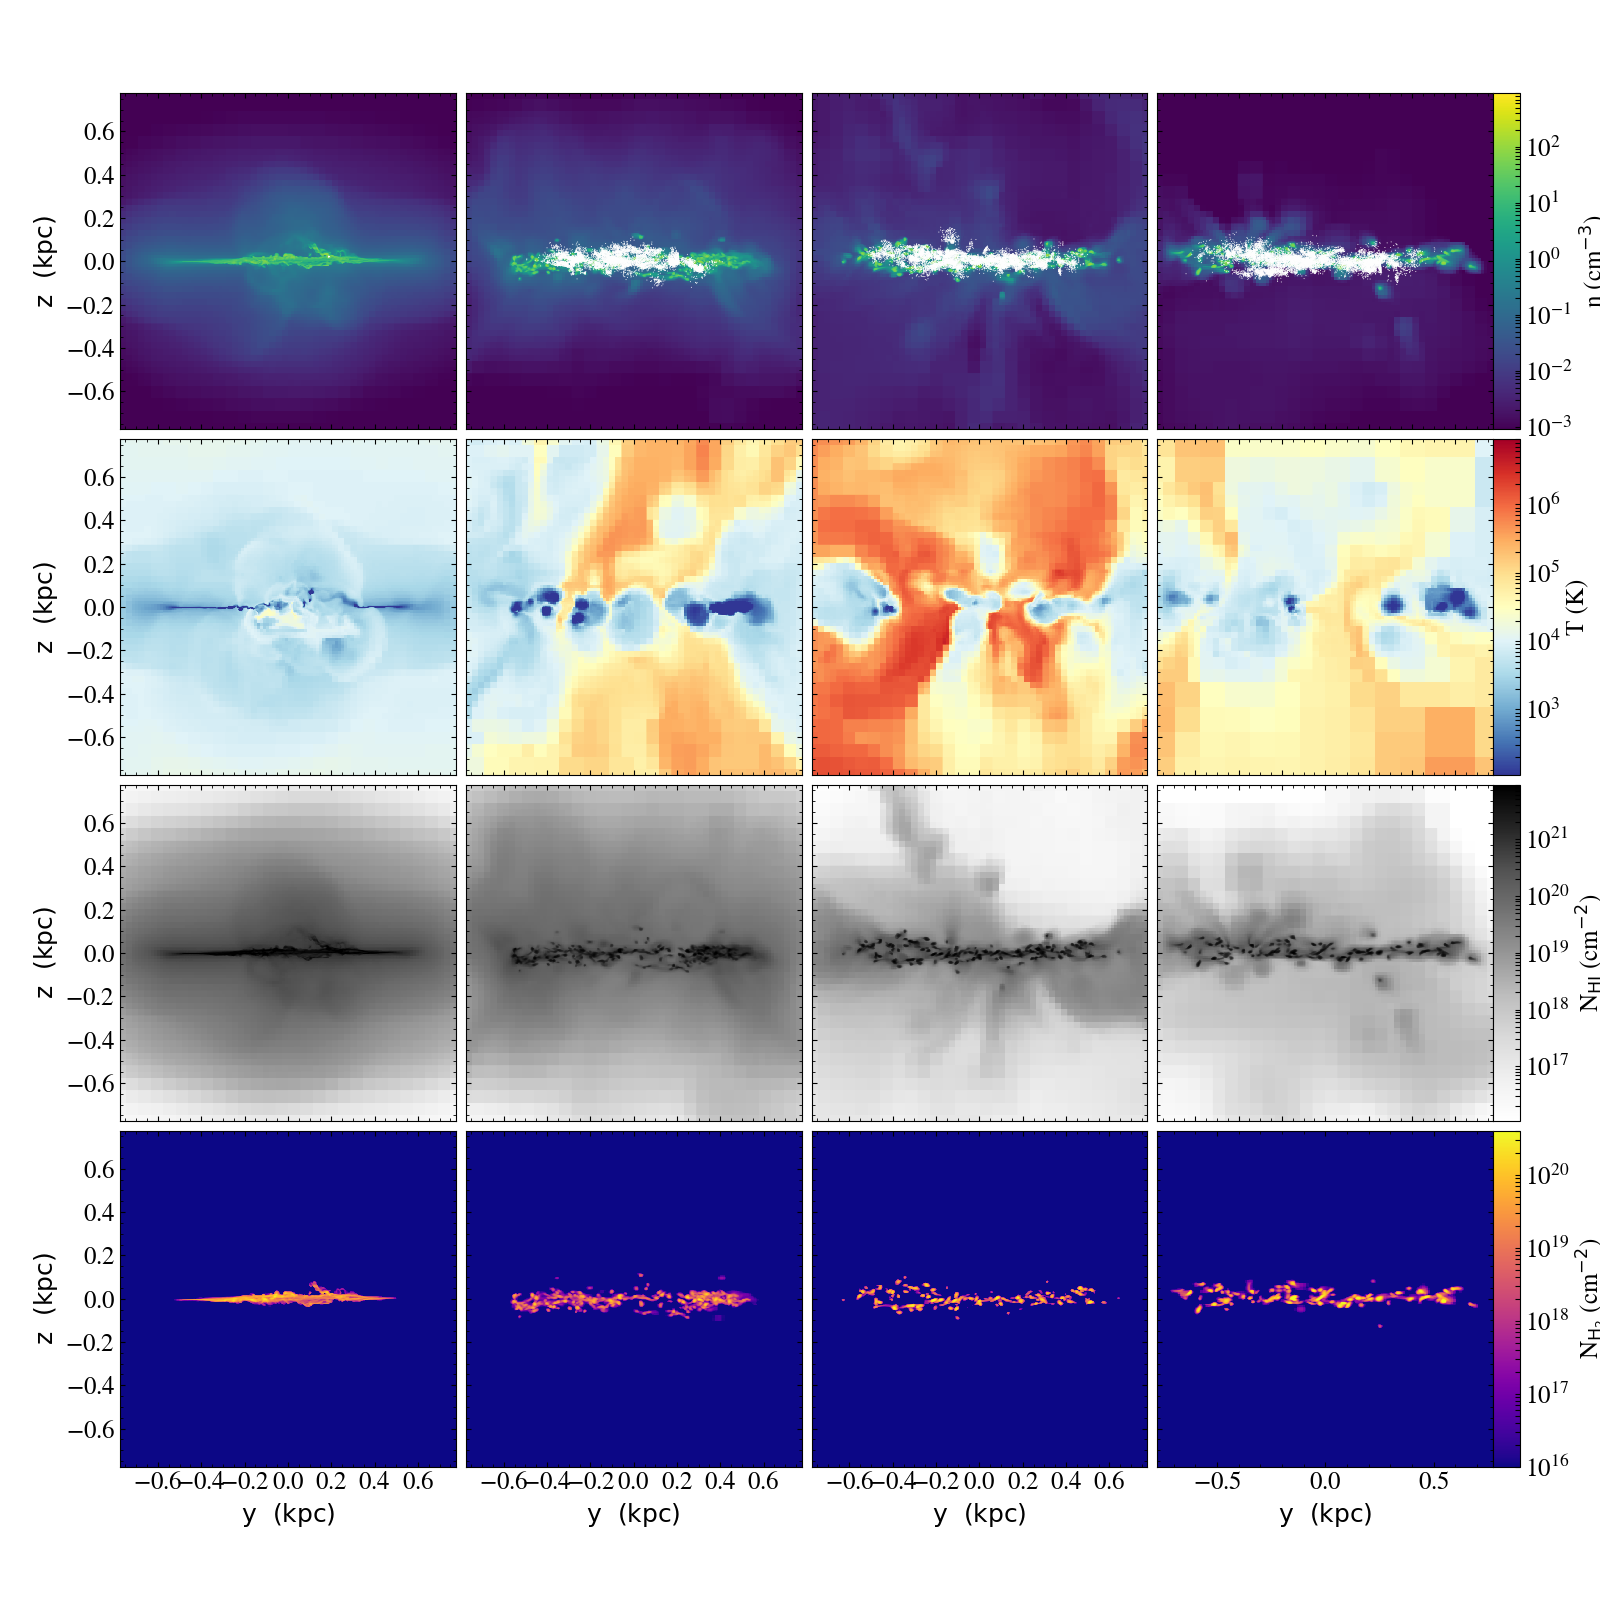
\includegraphics[width=0.975\linewidth]{figures/ch1/multiplot_4x4_x.png}
\caption{Edge-on views of our dwarf galaxy at four different times in its evolution, 0, 150, 300, and 500 Myr after the beginning of star formation. Shown are the density weighted projection of number density (top row), temperature slices (second row), HI column density (third row), and H$_2$ column density (fourth row). Each individual main sequence star particle is shown in the number density projections as a single white dot.}
\label{fig:ch1:panel_x}
\end{figure*}

The initially puffy gas distribution collapses to a thin disk, with scale heights between 10--30~pc, as shown by the blue line in Fig~\ref{fig:ch1:scale_height}. This figure shows the scale height of all gas in the disk, averaged over 20~Myr periods centered on each given time. Stellar feedback acts to heat up this initially thin disk substantially, creating typical scale heights of 50--120~pc. Towards the end of the simulation time, the half-light radius is $391 \pm 19$ pc, where the uncertainty represents the 1$\sigma$ variation in this quantity during the final 20 Myr. Although the disk remains thin beyond the half-light radius, with a scale height of around 50~pc, it is fully resolved at all radii. By the end of the simulation, the majority of the disk has a scale height of $\sim$100~pc.

Constraining the gas scale height in ultra-faint dwarf galaxies observationally is challenging. For Leo P, located at 1.7~Mpc, HI observations that are capable of detecting the diffuse HI throughout the galaxy have a resolution of 100--200 pc, with higher resolution observations identifying only the densest HI clumps in the galaxy \citep[e.g.][]{Bernstein-Cooper2014}. In the final column of Fig.~\ref{fig:ch1:panel_z}, the peak HI column density reaches $N_{\rm HI} = 9.4 \times 10^{21}$~cm$^{-2}$, but is located in dense regions with sizes $<$ 10$\sim$pc. With a resolution of 100~pc, the peak column density in an edge-on view is $N_{\rm HI} = 4.3 \times 10^{20}$~cm$^{-2}$, and $N_{\rm HI} = 2.8 \times 10^{20}$~cm$^{-2}$ in a face-on view. At 500 pc resolution, this corresponds to $N_{\rm HI} = 7.5 \times 10^{19}$~cm$^{-2}$, and $N_{\rm HI} = 6.2 \times 10^{19}$~cm$^{-2}$. These column densities are consistent with the resolution-dependent peak column densities found in the low mass dwarf galaxy sample of \cite{Teich2016}, and consistent with the observed peak column density of Leo P, $N_{\rm HI} = 6.5 \times 10^{20}$~cm$^{-2}$, observed with a spatial resolution of about 33~pc.

\begin{figure*}
\centering
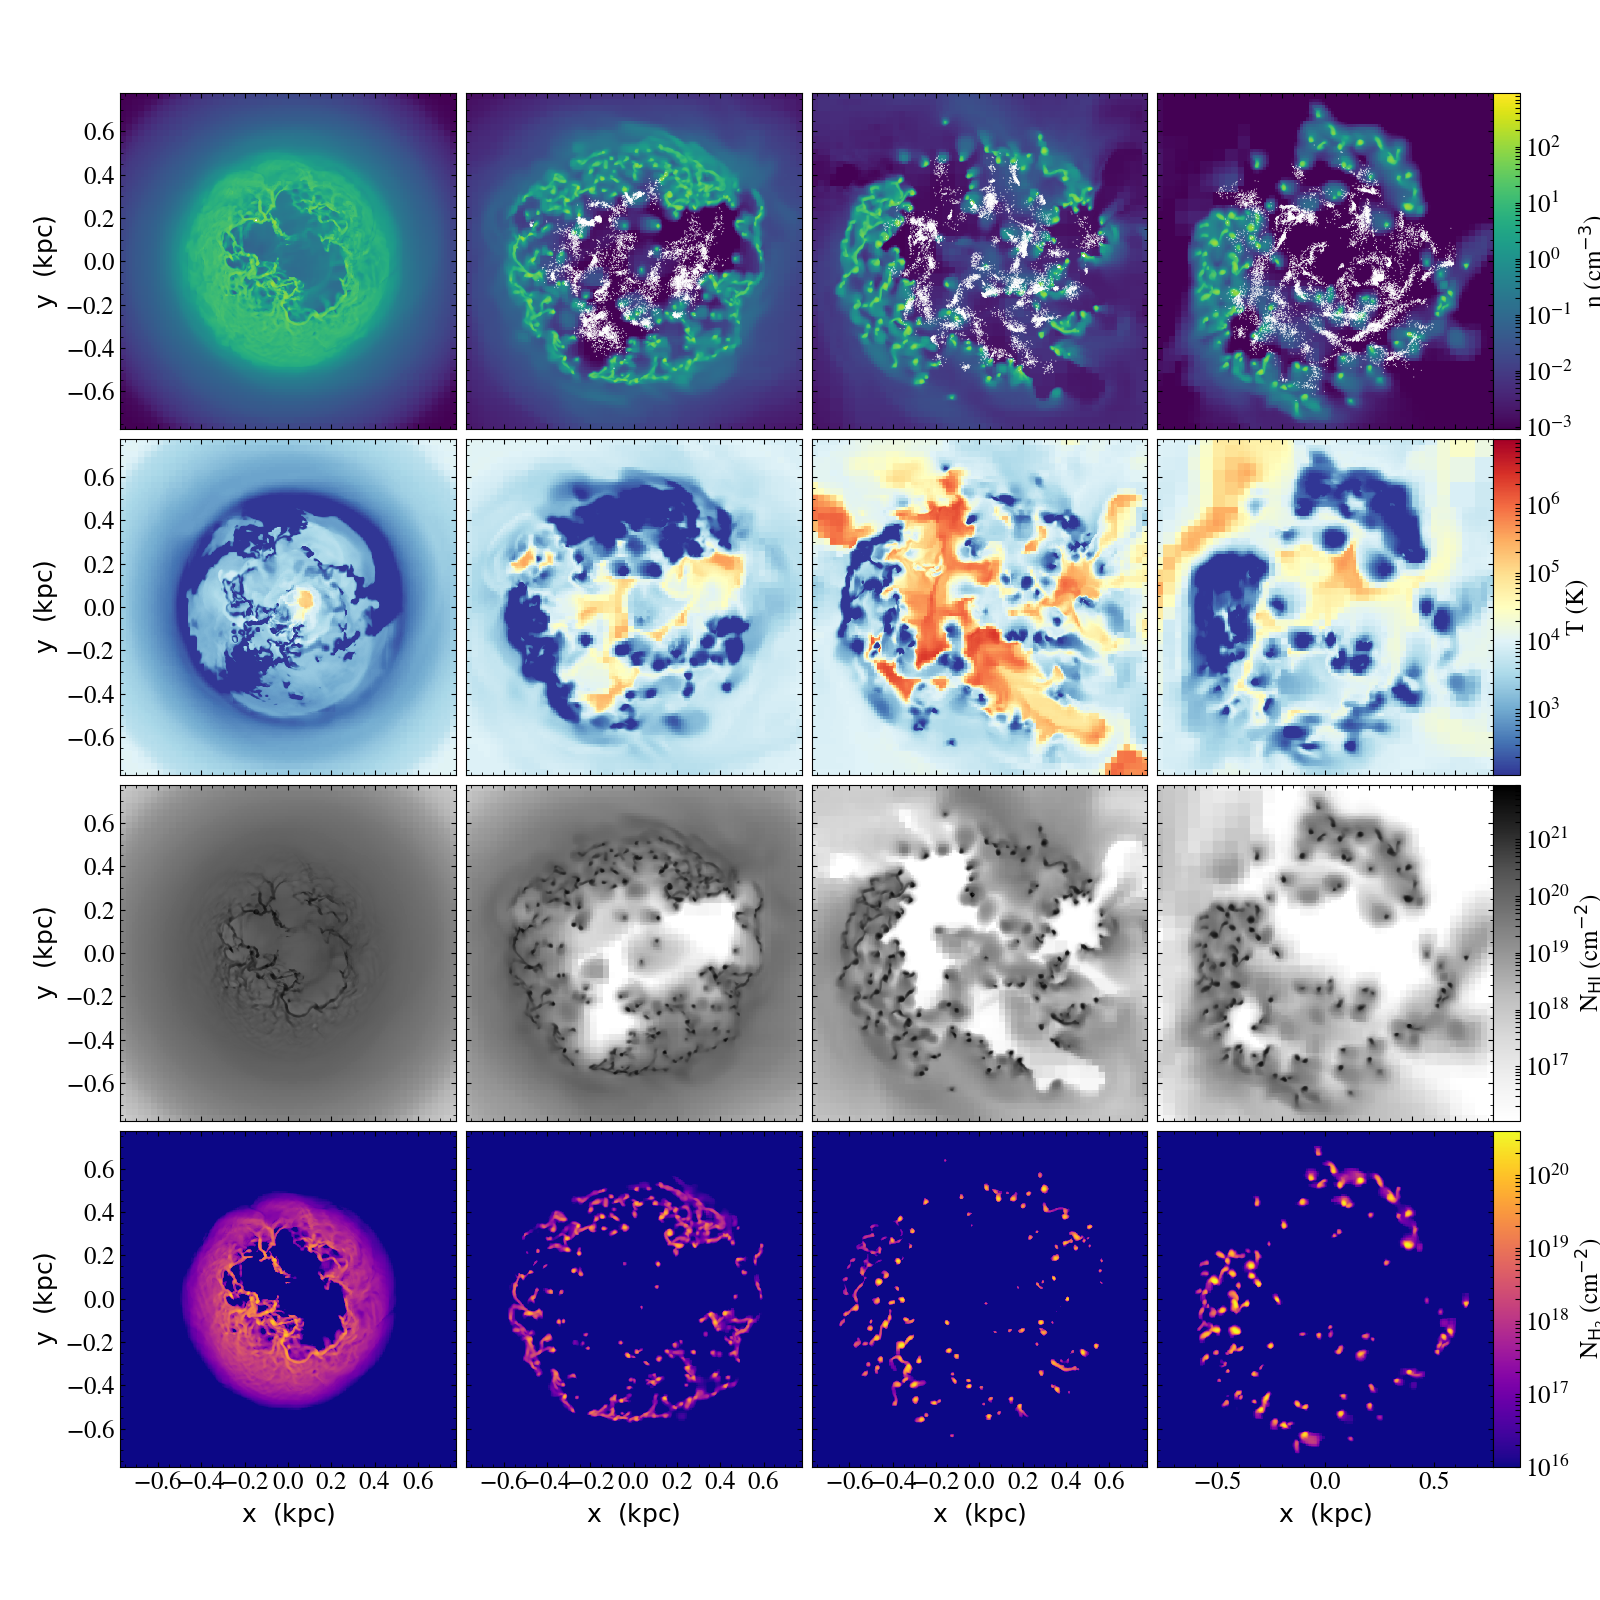
\includegraphics[width=0.975\linewidth]{figures/ch1/multiplot_4x4_z.png}
\caption{Same as Fig.~\ref{fig:ch1:panel_x}, but showing face-on views.}
\label{fig:ch1:panel_z}
\end{figure*}


\begin{figure}
\centering
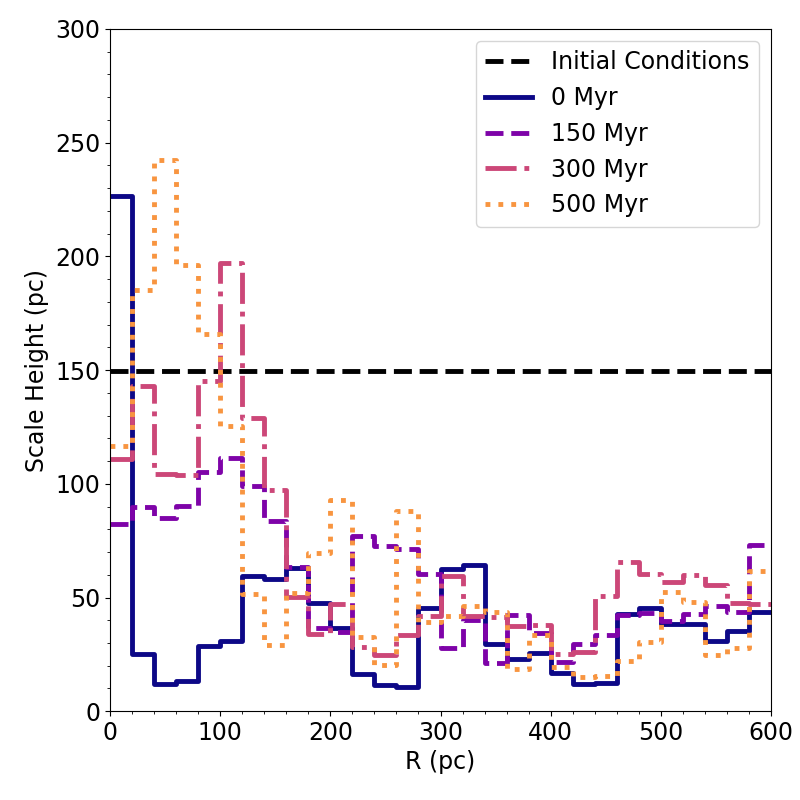
\includegraphics[width=0.975\linewidth]{figures/ch1/scale_height}
\caption{The total gas scale height at various times throughout the simulation. These times match the images in Figs.~\ref{fig:ch1:panel_x} and ~\ref{fig:ch1:panel_z}.}
\label{fig:ch1:scale_height}
\end{figure}

\subsection{Star Formation Rate and Mass Evolution}
\label{ch1:sec:sfr}

We present the star formation rate (SFR) and core collapse SN rate (SNR) evolution of our dwarf galaxy as measured in 10 Myr bins in the left panel of Fig.~\ref{fig:ch1:sfr_mass_evolution}.\footnote{We do not show the Type Ia rate as there have only been 16 by the end of the simulation.} Within the first 50 Myr of evolution the SFR rises quickly to nearly $10^{-3}$ M$_{\odot}$ yr$^{-1}$, declining to $\sim 3 \times 10^{-4}$~M$_{\odot}$~yr$^{-1}$ until a significant drop off at about 130 Myr. The remainder of the evolution is characterized by periods of little to no star formation interspersed with periods of continual, but low star formation around $10^{4}$~M$_{\odot}$~yr$^{-1}$. The SNR tracks the SFR with a time delay, with roughly one core collapse SNe per 100 M$_{\odot}$ of star formation. Averaging over the entire simulation time, we obtain  $<\rm{SFR}> = 1.19 \times 10^{-4}$ M$_{\odot}$ yr$^{-1}$. We discuss how the SFR of this galaxy compares to observed galaxies in Section~\ref{ch1:sec:observation}.

We note that the granularity in our star formation algorithm creates a lower limit to the SFR that depends on the period $\Delta t$ over which the SFR is measured. Since we produce stars in $\sim 100$~M$_{\odot}$ sets, the smallest value for our measured SFR is $\sim 100/ \Delta t$. For $\Delta t = 10$ Myr this is 10$^{-5}$ yr$^{-1}$. Removing the granularity requires a fundamental change in our star formation algorithm, likely at the cost of increased complexity and computational expense. Sink particles, which track pre-main sequence stellar mass accumulation, would be the most viable way to do this \citep[see for example ][]{Krumholz2004,Federrath2010,GongOstriker2013,BleulerTeyssier2014,Sormani2017}.

At initialization, all H and He of our dwarf galaxy is neutral, with no molecular hydrogen component. By the time of first star formation ($t=0$ in Fig.~\ref{fig:ch1:sfr_mass_evolution}), HI still dominates the mass of the galaxy, with a molecular hydrogen mass fraction of only $\sim$~0.3~\%. The molecular component declines rapidly as this gas is both converted into stars and is destroyed by stellar radiation feedback. For the remainder of the simulation, the H$_2$ mass generally increases,  with small fluctuations during periods of star formation, reaching a peak mass fraction of 5\% at 500~Myr. The growth of the molecular fraction is due in part to a decline in the total gas content of our galaxy from feedback-driven galactic winds. During these outflows, the densest gas, the molecular gas, is preferentially retained over the more diffuse ISM. Examining the molecular properties of the ISM in low mass dwarf galaxies in more detail is a vital avenue of future research, as there are significant observational uncertainties in deriving H$_2$ content of galaxies in this low metallicity regime \citep{Leroy2008,McQuinn2012,Amorin2016}. The molecular properties of our galaxy are discussed further in context with other works in Section~\ref{ch1:sec:observation}.

\begin{figure*}
\centering
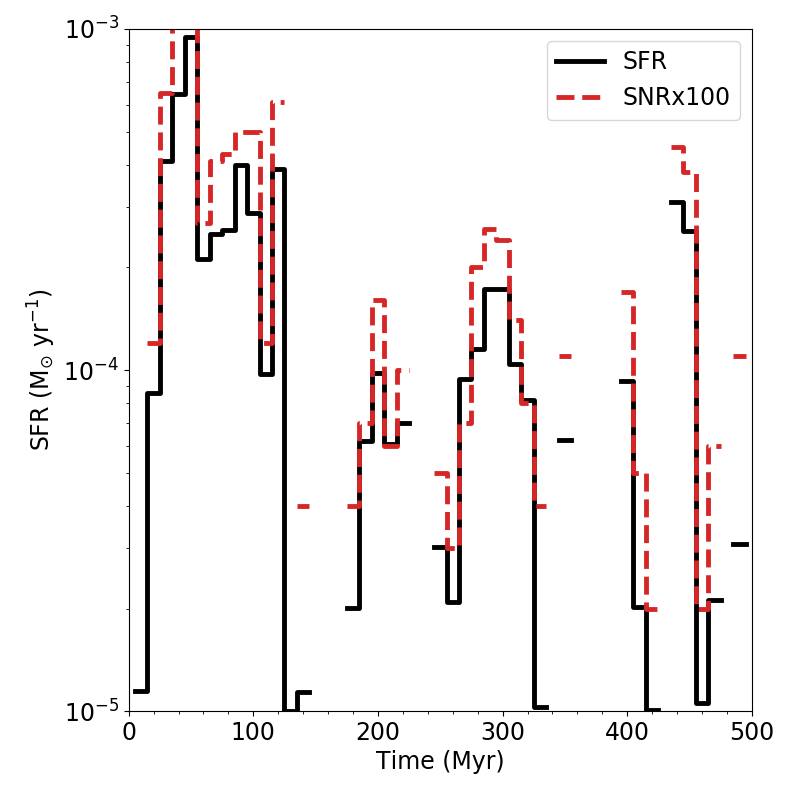
\includegraphics[width=0.475\linewidth]{figures/ch1/sfr_snrx100}
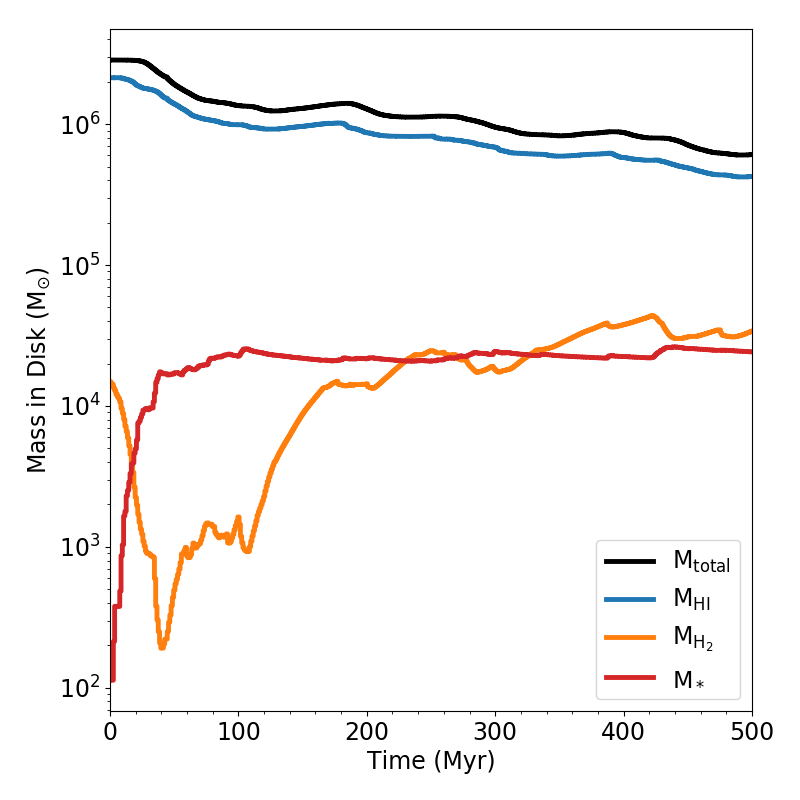
\includegraphics[width=0.475\linewidth]{figures/ch1/mass_evolution}
\caption{Left: The SFR and core collapse SN rate in our dwarf galaxy in 10 Myr bins. Broken portions of this histogram are time periods with no star formation or supernovae.  Note that the SN rate has been scaled by a factor of 100 to fit on the same vertical axis as the SFR. Right: The evolution of the total gas mass (black), HI mass (blue), H$_2$ mass (orange), and stellar mass (red) in the disk of our galaxy over time.}
\label{fig:ch1:sfr_mass_evolution}
\end{figure*}

\subsection{ISM Properties}
\label{ch1:sec:phase}

Our simulations include sufficient resolution and microphysics to capture a multi-phase medium within the ISM and halo of our simulated galaxy. We define five different gas phases following those defined in \citep{Draine2011}: molecular gas, cold neutral medium (CNM), warm neutral medium (WNM), warm ionized medium (WIM), and hot ionized medium (HIM). We emphasize that the molecular ISM phase is defined as all cells with M$_{\rm H_2}$/M$_{\rm gas} = $~f$_{\rm H_2} > 0.5$, and is thus somewhat different than simply considering the total H$_2$ content. By this definition, although our galaxy certainly contains molecular hydrogen, molecular gas as a phase does not exist; the peak f$_{\rm H_2}$ in any single cell remains below 30\%. See Appendix \ref{appendix:phases} for a quantitative definition of these phases. The properties of these phases are regulated by the complex interplay between cooling, turbulence, self-gravity, and radiative and shock heating from stellar feedback throughout the galaxy's evolution. Here we discuss the thermodynamic properties of the gas within the inner halo of our dwarf galaxy.

Fig.~\ref{fig:ch1:phase} shows the temperature-density distribution of all gas within 0.25 R$_{\rm vir}$ of the center of the galaxy, averaged over the time period 300--350~Myr. One can readily identify the two regimes containing most of the mass in the simulation: low density, warm gas produced through ionization and SN heating, and cold, high density gas that makes up most of the mass in the galaxy's disk (see Fig.~\ref{fig:ch1:ISM_evolution}). Several notable features of the distribution include: broad ranges of temperature even in quite dense gas, perhaps produced by photoionization and photoelectric heating, a substantial amount of extremely cold gas below 10~K, and the lack of well-defined thermal phases due to the complexity of both the heating and cooling in a turbulent medium. We note that we are likely missing important physics, such as cosmic ray heating and ionization, that would prevent the formation of the coldest gas in this diagram (below about 10~K), but we do not expect this to significantly alter our results. Our artificial temperature ceiling in diffuse gas (see Section~\ref{ch1:sec:hydro}) is seen clearly by the horizontal feature in the top left. The boxed regime in the lower right corner shows our star formation density and temperature threshold. Gas in this regime is rapidly consumed by star formation and subsequent feedback. Given the small size of our dwarf galaxy, the total amount of mass in this regime at any given instant can be small, but does appear in this time average.

\begin{figure}
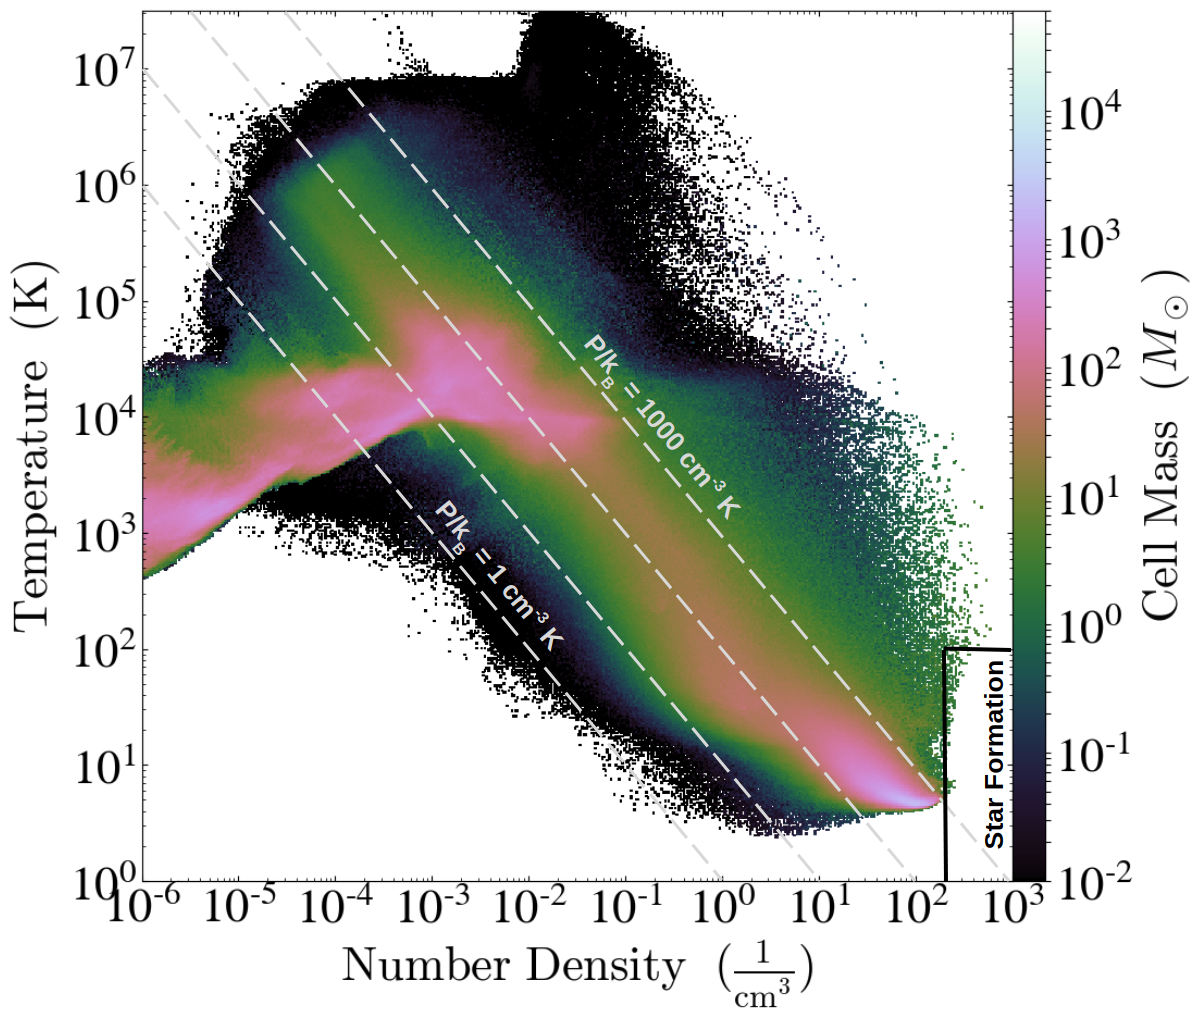
\includegraphics[width=0.95\linewidth]{figures/ch1/phase_diagram.png}
\caption{The temperature vs.\ number density phase diagram of our dwarf galaxy simulation showing all gas interior to 0.25~$R_{\rm vir}$, averaged over a 50~Myr period from t~=~300~Myr to t~=~350~Myr. The dashed lines are lines of constant pressure, separated by factors of 10. The region in the lower right corner indicates our density and temperature thresholds for star formation.}
\label{fig:ch1:phase}
\end{figure}

The mass of the ISM in our dwarf galaxy is dominated by the CNM for the entirety of the simulation, as shown in the left panel of Fig.~\ref{fig:ch1:ISM_evolution}. The mass fraction of the remaining phases are ordered by temperature, with the WNM as the next most-significant component. The WNM is initially comparable to the CNM, but comprises a mass fraction of about 0.1 by the end of the run. The WIM and HIM fluctuate significantly, corresponding to fluctuations in the SFR and associated feedback, but are subdominant throughout the simulation. During periods of peak stellar feedback, however, the WIM can reach a mass fraction above 0.1. Although the CNM dominates the mass fraction, it is a negligible component of the ISM volume, which is WIM dominated. However, the large, anti-correlated fluctuations in the WNM and HIM make these three phases often comparable. Together, these figures better quantify the general properties observed in the panel plots in Fig.~\ref{fig:ch1:panel_x} and Fig.~\ref{fig:ch1:panel_z}.

These results are in contrast with those found for the more massive dwarf galaxy modeled by \citet{Hu2016,Hu2017}. They find the mass and volume fraction of the ISM are nearly entirely dominated by warm gas (defined in those works as gas with 100~K$<$T$< 3\times 10^{4}$), with cold gas having between 1 and 10\% of the mass, and occupying negligible volume. Hot gas (defined as gas with $T > 3\times 10^{4}$~K) occupies 10\% of the volume, with negligible mass, in their galaxy, while our WIM alone occupies $>$ 50\% of the volume. Our lower mass, lower metallicity galaxy contains more cold gas (by mass fraction) and hot gas (by volume fraction) that seen in the more massive dwarf galaxy in these works. The driver of these differences, which are likely somewhat related to differences in the dark matter halo potential, will be investigated in future work. We have compared our cooling curves to those used in \citep{Hu2017} and found them to be comparable; though this could contribute to the differences, it is likely not the dominant source.

\begin{figure*}
%\centering
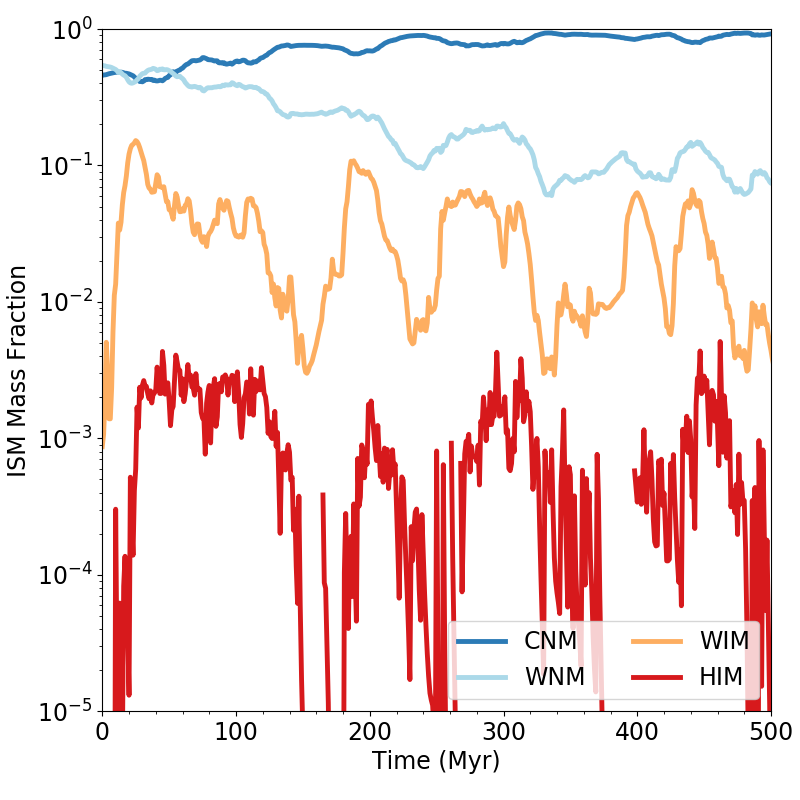
\includegraphics[width=0.45\linewidth]{figures/ch1/phase_mass_fraction_evolution_log.png}
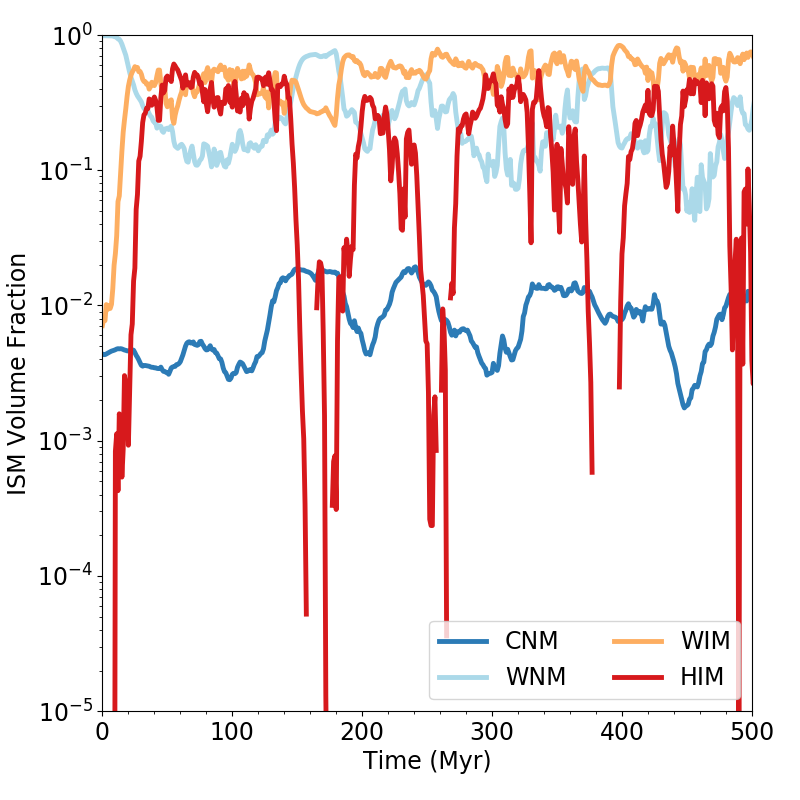
\includegraphics[width=0.45\linewidth]{figures/ch1/phase_volume_fraction_evolution_log.png}
\caption{The evolution of the mass and volume fractions for each phase of the model galaxy's ISM. See Appendix~\ref{appendix:phases} for definitions of each phase.}
\label{fig:ch1:ISM_evolution}
\end{figure*}

\subsection{Interstellar Radiation Field}
\label{ch1:sec:ISRF}

The interstellar radiation field (ISRF) of our galaxy varies dramatically in both space and time, as has been seen previously in works modeling varying radiation fields both as expected from stellar motions in our own galaxy \citep{Parravano2003}, and in models including radiation \citep[e.g.][]{Hu2017}. This is not particularly surprising in our low SFR regime, where there can be large fluctuations over time as individual massive stars form, move about, and evolve. In Fig.~\ref{fig:ch1:ISRF} we present azimuthally averaged radial profiles of the ISRF in various bands, time averaged over 100 Myr during the period of star formation from roughly 250--350~Myr. The top panel shows $G_{\rm o}$, the ISRF flux between 6--13.6~eV normalized to the value in the solar neighborhood of the Milky Way (see Sec.~\ref{ch1:sec:diffusive heating}). The averaged profile varies between values of 0.02 and 0.1, with peaks located at radii of the few active star formation regions. At any given radius, there is over a two order magnitude variation in the ISRF during this period of time.

The bottom panel gives the HI ionizing photon flux from stellar radiation. The ionizing radiation profile follows a similar trend, yet with significantly more variation, anywhere from two to four orders of magnitude. As this radiation is followed through radiative transfer, the profile encodes information about local attenuation by dense, neutral gas. This is the main driver of the differences between the two panels. The total fluctuation in both panels is due in part to the low-level, stochastic star formation in our galaxy. A higher star formation rate would produce a more regular population of massive stars and more uniform (in time) ISRF.

\begin{figure}
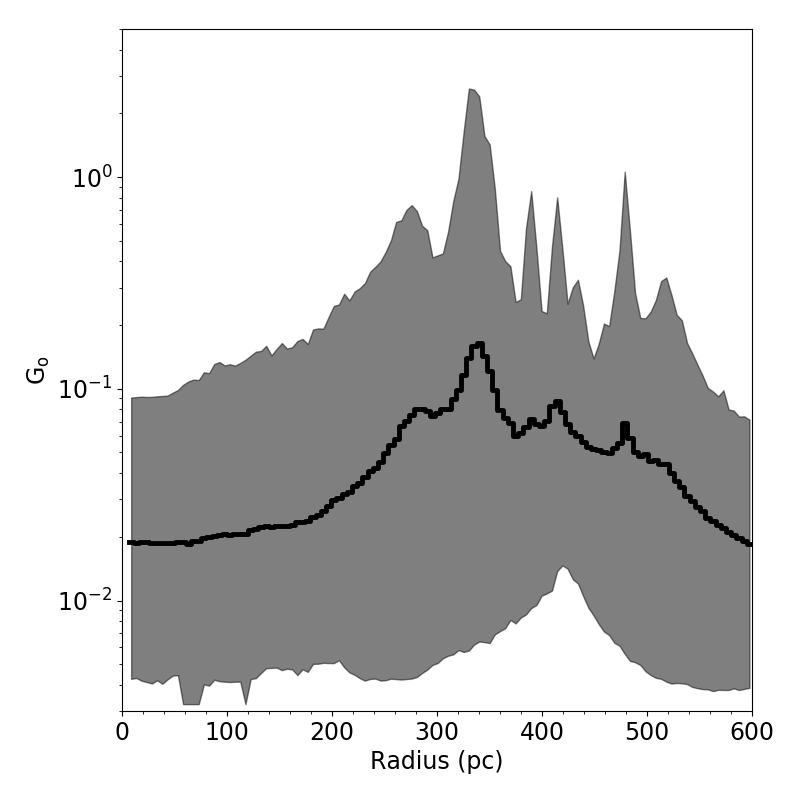
\includegraphics[width=0.95\linewidth]{figures/ch1/G_o_profile} \\
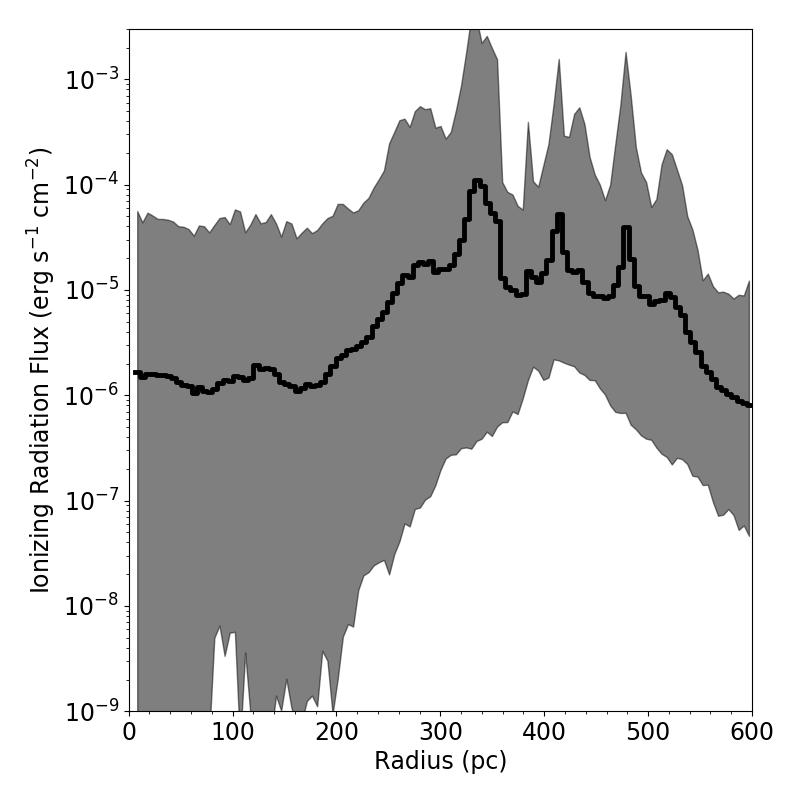
\includegraphics[width=0.95\linewidth]{figures/ch1/ionizing_photon_profile}
\caption{
Azimuthally averaged radial profiles of the ISRF in the mid-plane of our galaxy in two different bands, time-averaged over 50 Myr from 300 -- 350~Myr. Here we define the midplane as within 2.5~$dx$ of z = 0, or 4.5~pc. The top panel gives $G_{\rm o}$, the flux of radiation between 6--13.6 eV normalized to the value in the solar neighborhood, shaded between minimum and maximum values at each position, with the average shown as a black line. The bottom panel gives the HI ionizing stellar radiation flux. Since this radiation is tracked directly through radiative transfer, the minimum value at all radii is 0 at some point. For this reason we only shade between the first quartile and maximum values. HeI ionizing radiation is very similar to HI ionizing radiation, with a small vertical offset, and is not shown for clarity. In the top panel, the minimum of the vertical axis is the UVB value of $G_o$.}
\label{fig:ch1:ISRF}
\end{figure}

\begin{figure*}
%\centering
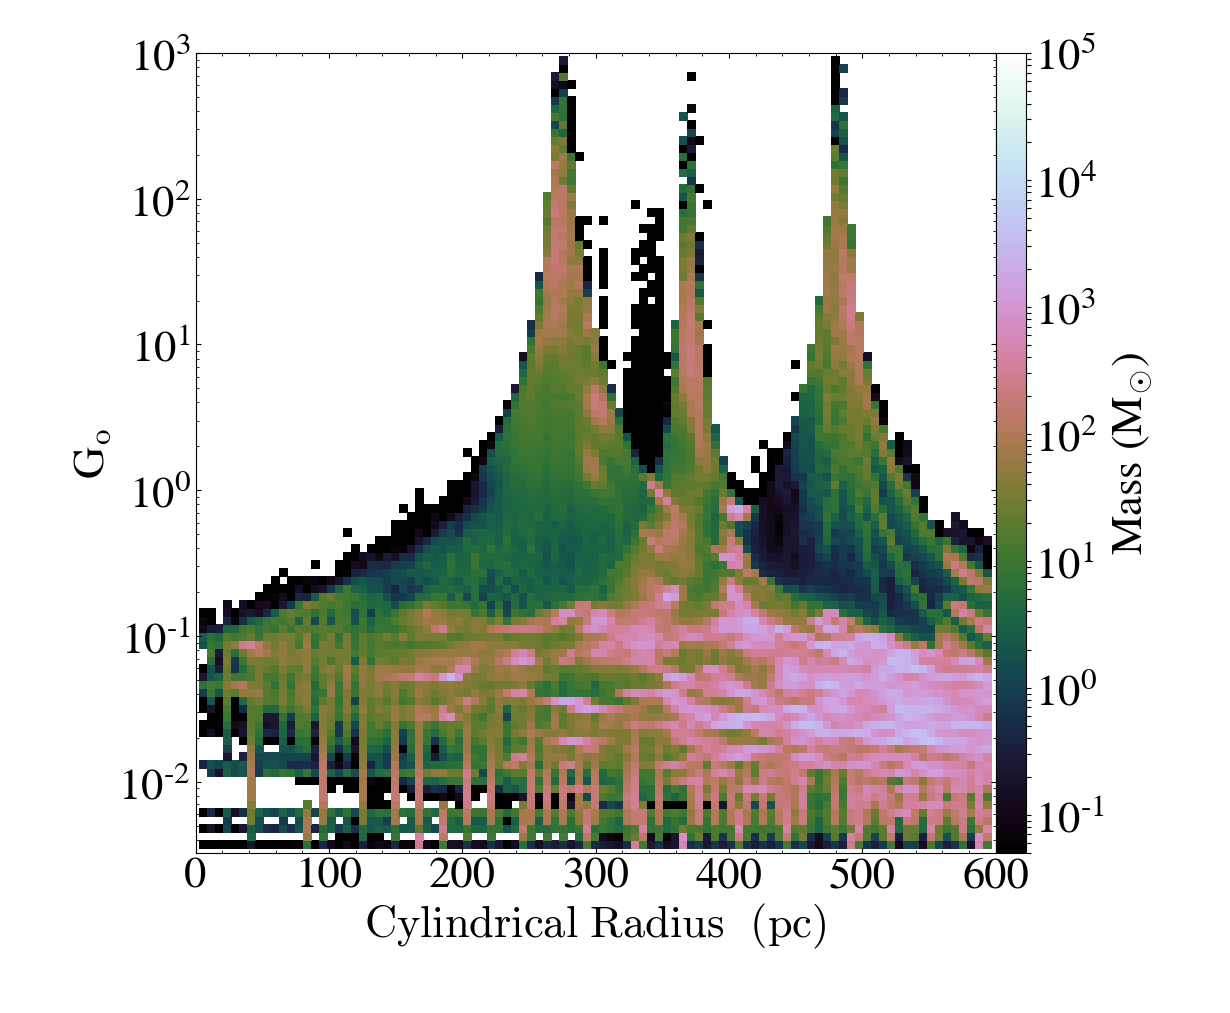
\includegraphics[width=0.45\linewidth]{figures/ch1/g_o_2D_phase}
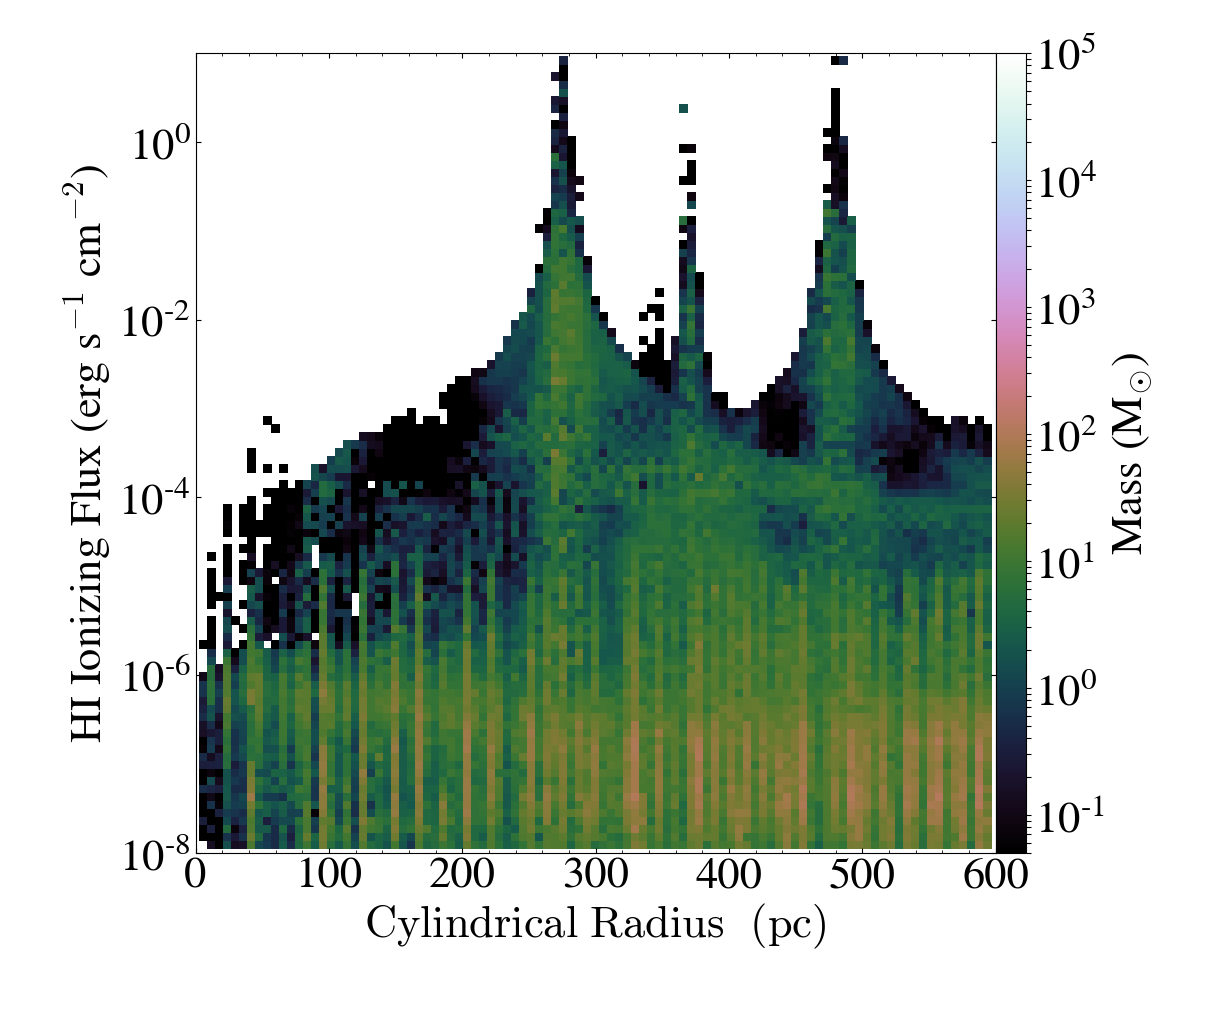
\includegraphics[width=0.45\linewidth]{figures/ch1/q_o_2D_phase}
\caption{Single-snapshot 2D radial profile plots at 300~Myr of the ISRF in two flux bands, $G_{\rm o}$ and HI ionizing radiation, illustrating the full dynamic range of radiation flux at a given radius in the galaxy. Here, we include all gas within the mid-plane of our dwarf galaxy. Since a majority of the mass of the galaxy is in the cold phase (see Fig.~\ref{fig:ch1:phase}), and is therefore optically thick to HI ionizing radiation, it does not show up in the HI ionizing radiation diagram. This gas readily appears in the $G_{\rm o}$ diagram since we assume it to be optically thin, though we do apply a localized shielding approximation.}
\label{fig:ch1:ISRF_2D}
\end{figure*}

To further quantify the local variations in these radiation fields, we present the full distribution of $G_{\rm o}$ and the HI ionizing flux in Fig.~\ref{fig:ch1:ISRF_2D} at a single snapshot at 300~Myr. This diagram shows how dramatic the increase in ISRF near young, massive stars is (the spikes in both diagrams), while much of the mid-plane sees an ISRF orders of magnitude lower. The striking contrast between the two diagrams is due to the shielding of the HI ionizing flux in the most massive (cold and dense) regions of the galaxy through the radiative transfer calculations; shielding of the FUV radiation is approximate and in general weaker, making these regions more prominent in the left hand figure (the pink/white clumps). From both of these diagrams, it is clear that the ISRF of a low mass dwarf galaxy varies greatly over time and space in a way that cannot be appropriately captured by an analytic profile. Although one could adopt an averaged radial profile to provide a realistic, global source of energy for thermal pressure support of the gas against collapse, it is unclear how sufficient this would be in suppressing star formation. In particular, the large increases around sites of recent star formation could be important sources of feedback to destroy molecular clouds and reduce their effective star formation efficiency. It remains to be seen which of these two modes of feedback is more important in regulating star formation.

\subsection{Outflow Properties}
\label{ch1:sec:outflows}

The recent FIRE cosmological simulations of dwarf galaxies over a range of dark matter halo masses find that they exhibit large outflows, with mass loading factors ($\eta = \dot{M}_{\rm out}/<\rm{SFR}>$) on order of 100--1000 \citep{Muratov2015}. However, comparable models of idealized dwarf galaxies with detailed feedback and physics treatments find more modest mass loading factors \citep{Hu2016,Hu2017}. In Fig.~\ref{fig:ch1:mass_outflow} we present the mass outflow and mass loading rates for our dwarf galaxy as a function of time, computed at five different positions from the galaxy. We follow \citet{Muratov2015} in defining the mass outflow rate at any given radius to be the sum of the outflow rate in all cells in a spherical annulus of width $dL$ centered at that radius,
\begin{equation} \label{eq:dotM}
\dot{M}_{\rm out} = \sum M_{\rm gas} \times v_{\rm r} / dL.
\end{equation}
We choose $dL = 0.1~R_{\rm vir}$, or 2.74 kpc.

The total mass outflow rates and mass loading factors at 0.1, 0.25, 0.5, and 1.0 $R_{\rm vir}$ are shown in Fig.~\ref{fig:ch1:mass_outflow}. Generally, other works use gigayear timescale measurements of the SFR to compute the mass loading factor. For consistency with those works, we use the 500~Myr average SFR for computing the mass loading factor. The outflow rate at 0.1 $R_{\rm vir}$ is high, corresponding to mass loading factors between 20--100 throughout the simulation time. This declines towards larger radii, however, with substantially less outflow past the virial radius. \citet{Muratov2015} finds typical mass loading factors at 0.25 R$_{\rm vir}$ on order of 20--40 for galaxies with $v_{c} = 30$ km s$^{-1}$ at low redshift, consistent with our results. The fluctuations in both of these panels are directly correlated with the SFR, with increased outflow during periods of star formation, and decreased outflow during periods of quiescence.

Interestingly, the v$_{\rm c}\sim$ 30 km s$^{-1}$ halos examined in \citet{Muratov2015} are more massive than the M$_{\rm vir} = 2.5\times 10^9$ M$_{\odot}$ halo examined here by a factor of a few. Using a fit provided in \citet{Muratov2015} to extrapolate and compare $\eta$ at fixed halo mass, one would expect mass loading factors on order of 100 at 0.25 R$_{\rm vir}$ for our dwarf galaxy, a factor of a few higher than what we find. These differences could be attributed to our lack of cosmological evolution in these isolated simulations, but ultimately requires a larger set of dwarf galaxy simulations to make a more robust comparison. We note, however, that our results are closer to the \citet{Muratov2015} results than those in \citet{Hu2016,Hu2017}, which find lower mass loading factors even closer to the disk, at 0.05 $R_{\rm vir}$, between 1 and 10 for a dwarf galaxy with M$_{\rm vir} = 10^{10}$ M$_{\odot}$; certainly this implies even smaller mass loading factors at 0.25 $R_{\rm vir}$.

\begin{figure*}
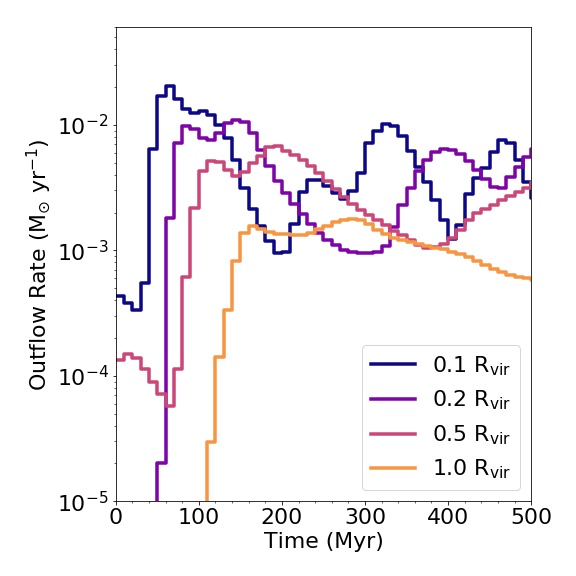
\includegraphics[width=0.45\linewidth]{figures/ch1/total_mass_outflow}
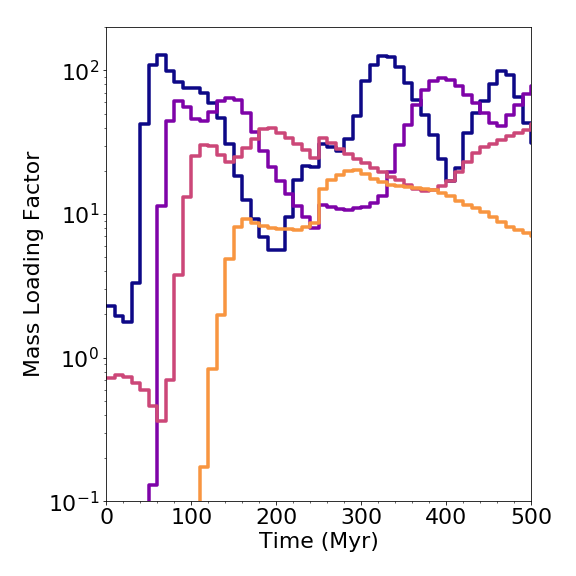
\includegraphics[width=0.45\linewidth]{figures/ch1/total_mass_loading}
\caption{Spherical mass outflow rates (Eq.~[\ref{eq:dotM}]) and mass loading rates over time at 4 different radii from the galaxy.}
\label{fig:ch1:mass_outflow}
\end{figure*}

Detailed outflow properties, beyond outflow rates and mass loading factors, can help discriminate between the model dependent feedback physics included in galaxy simulations. In Fig.~\ref{fig:ch1:outflow_velocity} we present radial velocity distributions of all material outside our dwarf galaxy's disk, and within the halo, broken into three gas phases. Gas with a negative velocity is moving towards the center of the halo. Roughly 25\% of this mass is inflowing, mostly with modest negative velocities, and corresponds to previously ejected gas mixing and recycling throughout the halo. Half of the outflowing gas (positive velocities) is moving at velocities below 30 km s$^{-1}$, 75\% at velocities below 70 km s$^{-1}$, and 95\% at velocities below 100 km s$^{-1}$. Although the mass contained in the tails of these distributions is a sub-dominant fraction of the total, there is still a non-negligible amount of gas moving at velocities of a few hundreds of km/s, with a peak velocity of over 700 km s$^{-1}$. The WNM and WIM together dominate the mass of both the inflowing and outflowing gas, with the WIM and HIM dominating at velocities above 200 km s$^{-1}$. The dominant launching mechanism in this simulation is SN feedback, which generates a rapidly moving and volume-filling WIM and HIM, consistent with the results in \citet{Hu2016,Hu2017}. However, as shown, the HIM, which is mostly the SN ejecta itself, comprises very little of the outflow by mass. Most of the outflowing gas (by mass) comes from the warm phase, pushed out by the high pressure, fast moving HIM. Some of this warm gas certainly originates from adiabatically and radiatively cooled HIM, however. The amount of transfer between phases in the halo of our galaxy will be investigated in future work.

\begin{figure}
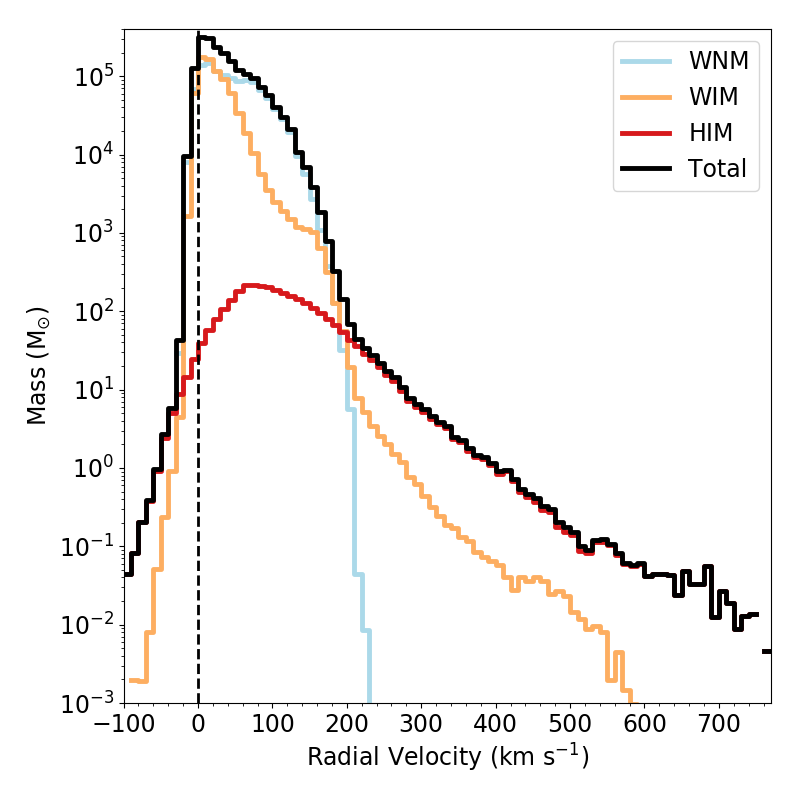
\includegraphics[width=0.95\linewidth]{figures/ch1/velocity_distribution_time_average}
\caption{The time averaged radial velocity distribution of outflowing material external to the disk and within the virial radius of our dwarf galaxy. This is averaged over the same time interval as Fig.~\ref{fig:ch1:ISRF}. The outflowing material is multiphase, broken into WNM, WIM, and HIM. See Section~\ref{ch1:sec:phase} for definitions of these regimes. We note that WNM is often labeled simply as ``cold'', or gas below $T = 10^{4}$~K. There is little to no outflowing mass in the CNM.}
\label{fig:ch1:outflow_velocity}
\end{figure}

\subsection{Metal Evolution}
\label{ch1:sec:chemical evolution}

\subsubsection{Metal Enriched Outflows}
Dwarf galaxies efficiently, and preferentially, eject metals released in stellar feedback from their shallow potential wells \citep{MacLowFerrara1999,FerraraTolstoy2000}. This has been better quantified recently both observationally \citep[e.g.][]{Kirby2011-metals,Zahid2012,Peeples2014,McQuinn2015} and with more detailed cosmological simulations \citep{Simpson2013,Angles-Alcazar2017,Muratov2017}. In the top panel of Fig.~\ref{fig:ch1:metal_evolution}, we give the metal mass loading factor for our galaxy over time, at the same radii as in Fig.~\ref{fig:ch1:mass_outflow}. The parameter used to quantify metal outflow efficiencies varies among works. Here, we define the metal mass loading factor as the metal outflow rate divided by the metal production rate, or
\begin{equation} \label{eq:eta-metal}
\eta_{\rm metal} = \frac{\dot{M}_{\rm metal}}{\rm{SFR} \times (M_{\rm metal}/M_{*})},
\end{equation}
where $\dot{M}_{\rm metal}$ is the metal mass outflow rate, $M_{\rm metal}$ is the total mass in metals produced, and $M_{*}$ is the total mass in stars. These metal loading factors fluctuate significantly with the SFR, just as was shown in Fig.~\ref{fig:ch1:mass_outflow}, reaching a minimum of about 0.05, but peaking at around 5. On average, over the simulation time, $\eta_{\rm metal}$ is below unity (around 0.5). Recent simulations of outflows from a Milky Way type disk indicate typical $\eta_{\rm metal}$ comparable to our results, usually between 0.5 and 1 \citep{Li2017,Fielding2017}. \cite{Muratov2017} computes a slightly different quantity for their galaxies, the normalized metal outflow rate $\eta_{Z} = \dot{M}_{\rm metal}/{\rm SFR}$, finding values of about 0.02 at 0.25~$R_{\rm vir}$ regardless of galaxy circular velocity. Our galaxy is consistent with this value, with an average $\eta_Z = 0.015$, fluctuating between 0.007 and 0.02.

\begin{figure}
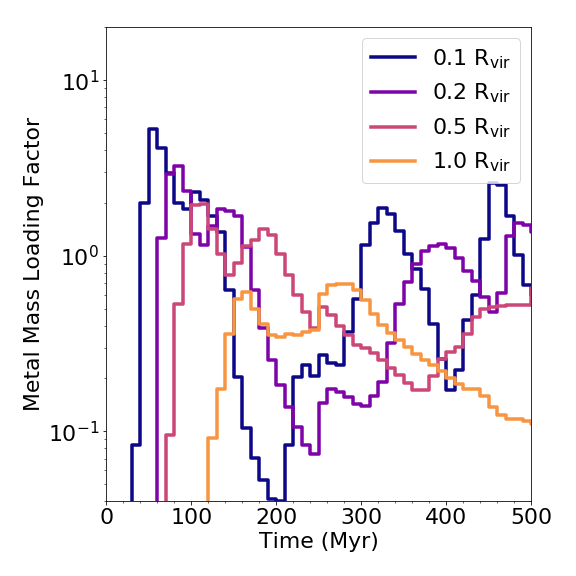
\includegraphics[width=0.9\linewidth]{figures/ch1/metal_mass_loading} \\
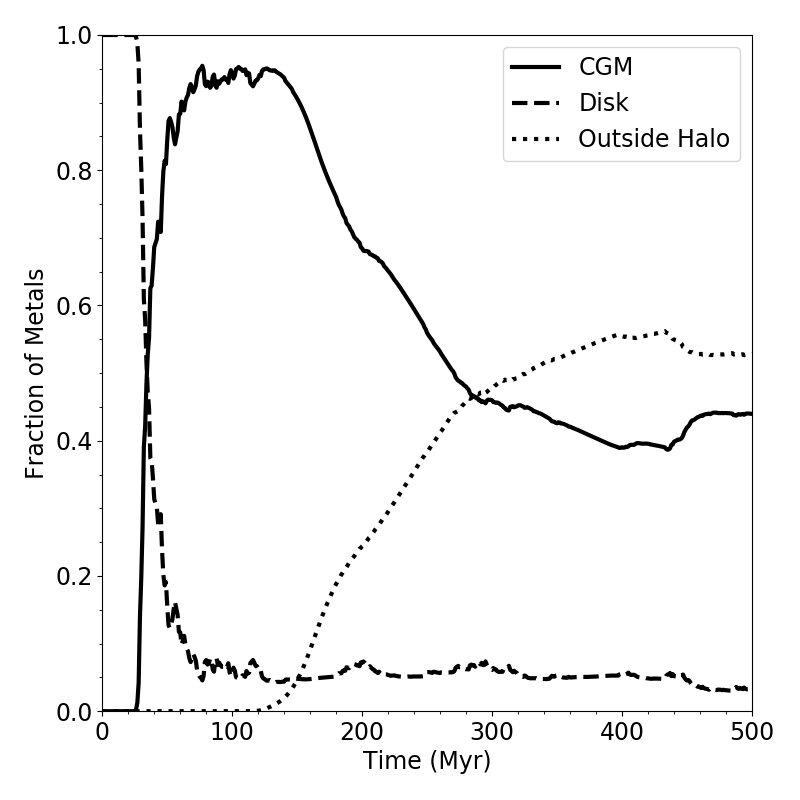
\includegraphics[width=0.9\linewidth]{figures/ch1/metal_retention}
\caption{{\bf Top}: Metal mass loading factor (see Eq.[~\ref{eq:eta-metal}]) at the same radii as in Fig.~\ref{fig:ch1:mass_outflow}. This is the ratio between the metal outflow rate and the metal production rate. {\bf Bottom}: The fraction of metals contained in the disk, CGM, and outside the halo of our dwarf galaxy over time. In both panels, we consider the total mass of all individually tracked metal species, which is zero at initialization, not the aggregate total metallicity field, which is non-zero at initialization.}
\label{fig:ch1:metal_evolution}
\end{figure}

These large metal mass loading factors indicate that a majority of the metals produced in our dwarf galaxy are ejected from the disk. This is quantified in the lower panel of Fig.~\ref{fig:ch1:metal_evolution}, where we show the mass fraction of metals in the disk, circumgalactic medium (CGM), and outside the virial radius of our galaxy over time. After the first 20 Myr, SN-driven winds rapidly drive out large quantities of metals from the disk and into the galaxy's halo. This continues throughout the simulation, with only $\sim$4\% of produced metals residing in the disk of the galaxy. It only takes 150 Myr for some metals to reach the virial radius of the halo, with a steadily increasing fraction continually leaving the virial radius until about 350 Myr where the fraction levels off to just above 50\%. Likewise, the CGM metal content continually decreases until the end of the simulation from loss through the virial radius of the halo. See Section~\ref{ch1:sec:obs_metals} for further discussion.

\subsubsection{Differential Evolution of Elements Within the ISM}
It is important to understand how metals from each source of stellar yields enrich the ISM. Observations of more massive dwarf galaxies than those simulated here indicate fairly uniform radial gas-phase metallicity profiles, even beyond the stellar radius \citep[e.g.][]{Werk2011,Belfiore2017}. This requires that metal mixing and transport occur on hundred megayear timescales, much more rapidly than the gigayear timescale expected from assuming transport at the cold gas sound speed. Therefore, either metals are transported first through a hot phase with high sound speed, or through efficient turbulent mixing within the ISM \citep[e.g.][]{Avillez2002,Tassis2008,YangKrumholz2012}. It remains uncertain how metal abundances vary in detail within these galaxies, beyond one-dimensional radial profiles, and whether or not abundance distributions depend on the metal species. It is even more unclear how metals are transported and distributed within low-mass dwarf galaxies, which generally host too few \ion{H}{2} regions for a detailed examination.

We demonstrate the power of our simulations, which capture a realistic ISM at high resolution with multiple feedback sources, by addressing these questions in Fig~\ref{fig:ch1:metal_slices}. The left panel gives the abundance ratio of N to O throughout the ISM. The right
two panels give the slices of number density (top right) and temperature (bottom right) in the mid-plane of a portion of our dwarf galaxy. These show regions with dense, cold gas clouds ($n \sim 100~\rm{cm}^{-2}$, $T \lesssim 100~$K) connected by cold filaments, warm, diffuse gas ($n\sim 0.1$~cm$^{-3}$, $T\sim 10^{4}$~K), and hot gas from a recent SN explosion ($T\sim10^{6}$~K).

\begin{figure*}
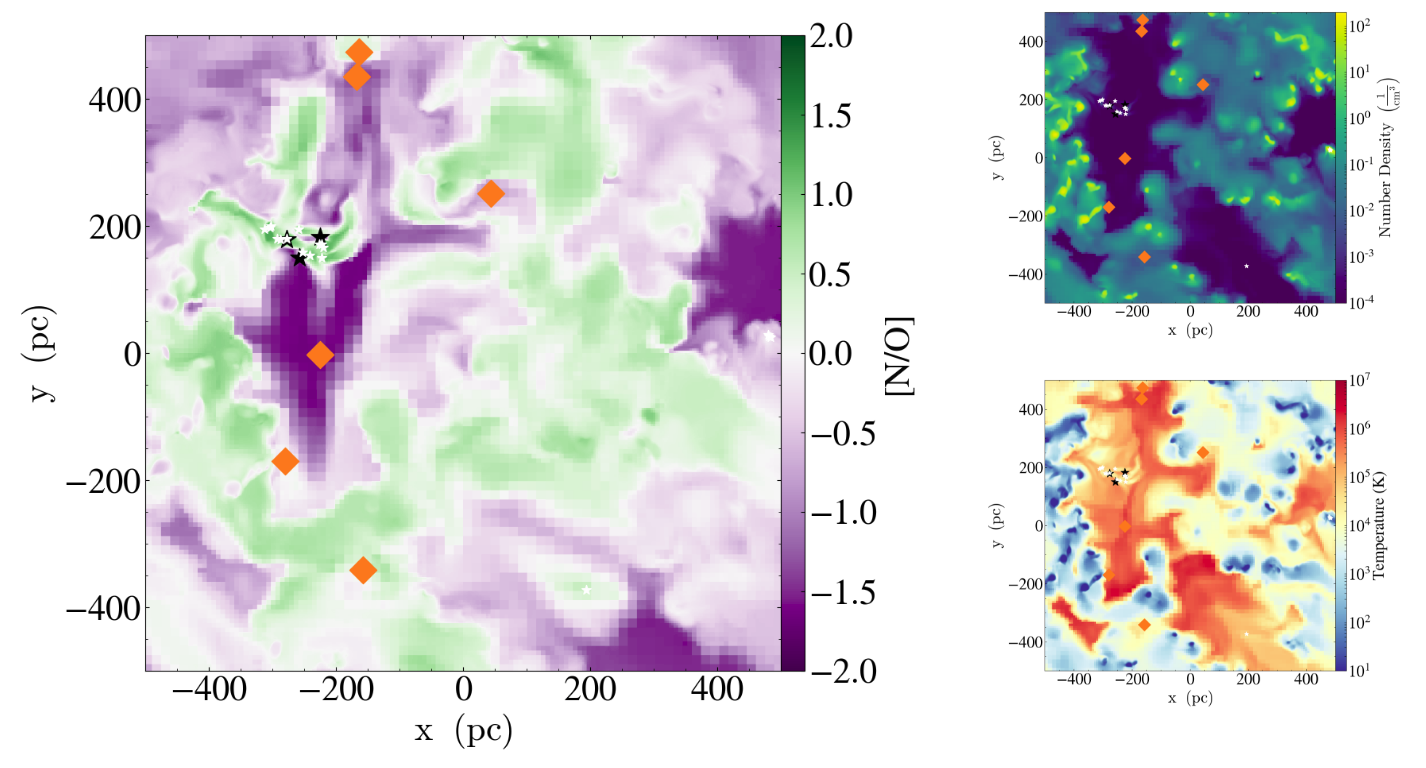
\includegraphics[width=0.98\linewidth]{figures/ch1/log_NO_panel}
\caption{Three slices in the mid-plane of our dwarf galaxy at 300~Myr after the start of star formation showing the variation in gas phase metal abundances. The left slice gives the ratio of the abundance between N and O, normalized to the solar abundance, while the number density and temperature are shown on the right. In each, we mark massive stars with active stellar winds as white points and SNe and AGB-phase enrichment events that occurred in the preceding 5 Myr as black stars and orange diamonds respectively.}
\label{fig:ch1:metal_slices}
\end{figure*}

As shown in the left panel, [N/O] varies significantly over this section of the ISM with notable differences across the various phases and ISM structures. The hottest gas, dominated by recent supernova explosions is overabundant in oxygen, relative to solar (purple). However, the relative abundance of nitrogen increases in the WIM and WNM, being overabundant relative to solar (green).

At our adopted metallicity, nitrogen is predominantly produced in AGB star winds, with very little production in core collapse SNe and winds from more massive stars. Therefore, nitrogen is injected into the ISM with significantly less energy ($v \sim 10$~km~s$^{-1}$) than elements produced in SNe, like oxygen, ($v\sim 10^3$~km~s$^{-1}$). Given the variations in Fig.~\ref{fig:ch1:metal_slices}, the energetic differences between injection sources can drive abundance variations within the ISM of our dwarf galaxy. The regions most rich in N are sites of recent AGB winds that have yet to mix with the rest of the ISM. This suggests that metal mixing within the ISM (and also metal ejection from the ISM) is species dependent. A more detailed analysis is beyond the scope of this work, but we investigate this in detail in \cite{Emerick2018b}.

\section{Discussion}
\label{ch1:sec:discussion}

\subsection{Comparison to Observed Low Mass Dwarf Galaxies}
\label{ch1:sec:observation}

As noted in Section~\ref{ch1:sec:IC}, our galaxy model is not intended to directly reproduce the observed properties of Local Group ultra-faint dwarfs. Notably, our initial conditions neglect a pre-existing stellar population and are only followed for 500~Myr, a fraction of the age of $z = 0$ dwarf galaxies. However, we can still place our model in context with observations using simple comparisons to the star formation rate (Section~\ref{ch1:sec:gas_sf}), molecular gas (Section~\ref{ch1:sec:molecular gas content}), and metal retention fraction (Section~\ref{ch1:sec:obs_metals}) properties of observed dwarf galaxies. We show that these properties are broadly consistent with observations.

\subsubsection{Gas and Star Formation}
\label{ch1:sec:gas_sf}

The observational sample of isolated, gaseous, low mass dwarf galaxies is limited compared to more massive galaxies, but has improved substantially with recent blind and targeted HI surveys \citep[e.g.][]{Giovanelli2005, Geha2006, Geha2012, Walter2008, Cannon2011, Haynes2011, Hunter2012, Bradford2015, James2015, Tollerud2015, Sand2015, Wang2017}. However, the sample of isolated, gaseous dwarf galaxies with $M_{*} < 10^{7}$~M$_{\odot}$ remains small. In Figure ~\ref{fig:ch1:KS} we show where our galaxy lies relative to the observed Kennicutt-Schmidt relation and extended Schmidt law for low mass galaxies. In both diagrams, our simulations are given by the colored points, sampled every megayear throughout the entire simulation.

Although simple to measure in simulations, these quantities are challenging to directly compare to observations. We have attempted to make a reasonable analog to how $\Sigma_{\rm sfr}$ and $\Sigma_{\rm gas}$ are measured observationally for low mass dwarfs \citet[see ][]{Roychowdhury2014}. We define $\Sigma_{\rm sfr} = \dot{M}_{*,10} / A_{*,10}$, where $\dot{M}_{*,10}$ is the SFR measured over the preceding 10~Myr, and $A_{*,10}$ is the area of the disk within the radius of the outermost star formed within the previous 10 Myr. Likewise, $\Sigma_{\rm gas} = M_{\rm gas,10} / A_{*,10}$, where M$_{\rm gas,10}$ is the total gas mass within this defined disk. However, the total gas content cannot be determined observationally. To match this limitation, we follow \cite{Roychowdhury2014} and take $\Sigma_{\rm gas, obs} = 1.34 \times \Sigma_{\rm HI}$, where the factor 1.34 attempts to account for He. We note that there is generally no correction made for any possible H$_{\rm 2}$ or HII content. As shown in Section~\ref{ch1:sec:molecular gas content}, these components may be significant.

\begin{figure*}
\centering
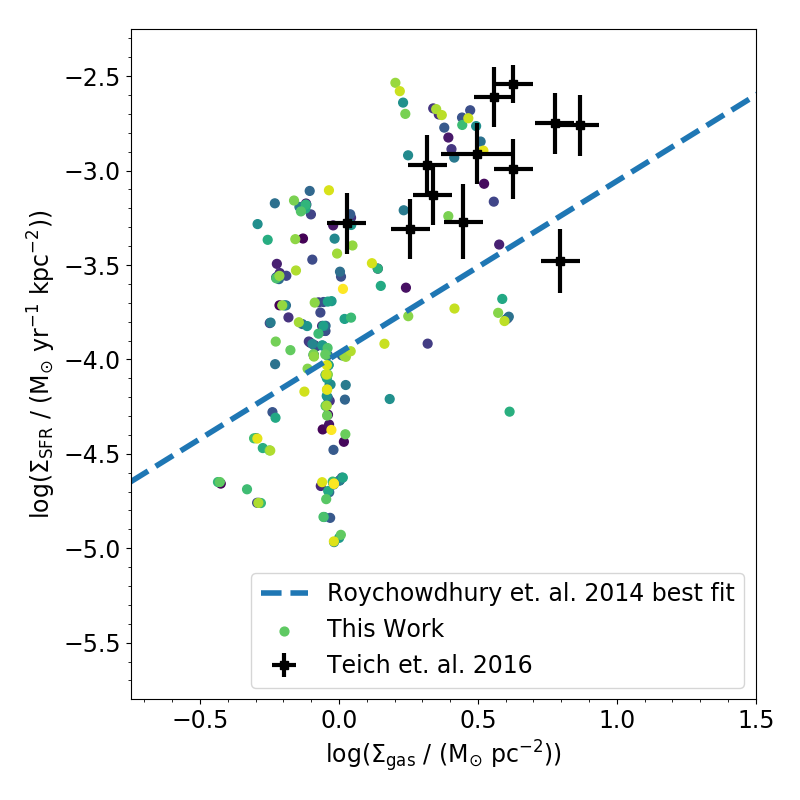
\includegraphics[width=0.475\linewidth]{figures/ch1/all_gas_schmidt_law_evolution.png}
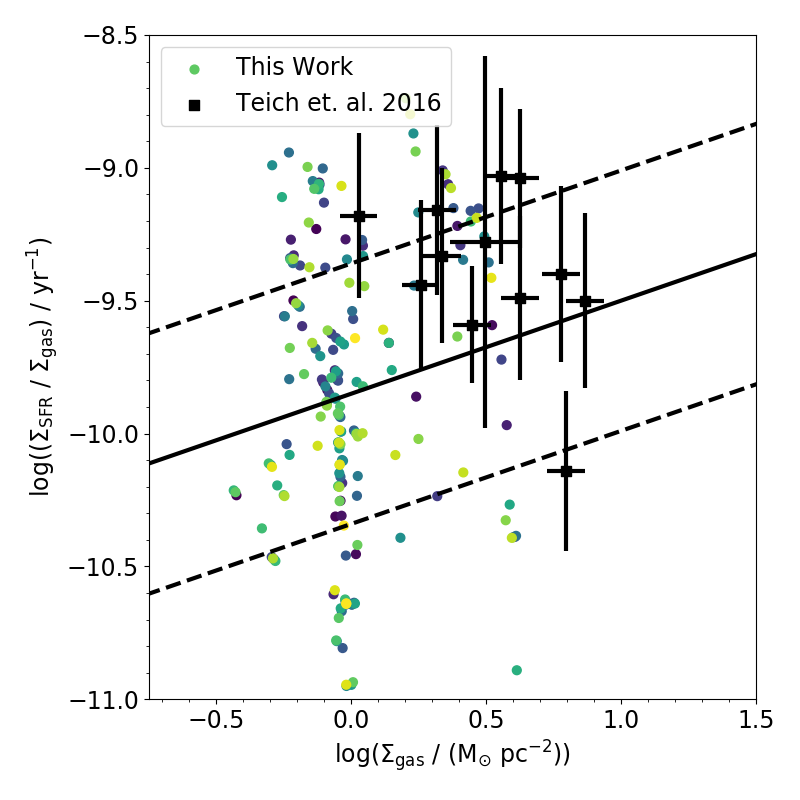
\includegraphics[width=0.475\linewidth]{figures/ch1/all_gas_efficiency_evolution.png}
\caption{The Kennicutt-Schmidt law (left) and extended Schmidt law (right) relationships for our galaxy as measured every megayear, plotted as points colored by time, with dark / purple early and light / green late. See text for details of the calculation. Recent observations from the SHIELD sample \protect\citep{Teich2016} are plotted as black points with error bars. On the left, we also give the best fit line to galaxies from the FIGGS sample from \protect\cite{Roychowdhury2014}, and on the right we also show the best fit line and 1 $\sigma$ errors from \protect\cite{Shi2011}. There is no clear correlation with time in this diagram.}
\label{fig:ch1:KS}
\end{figure*}

We include recent observational constraints on these relationships in Figure ~\ref{fig:ch1:KS}. Our galaxy fluctuates significantly about both relationships with no clear trends in time. However, in both cases, it is consistent with the available observational sample. At times our galaxy exhibits gas surface densities below the observational constraints. The trend is still consistent with higher densities at this point, but with a larger scatter towards lower star formation rate densities and efficiencies.

In constructing our galaxy model, we employed \textit{no} tuning of the underlying physics, adopting only canonical values for any available free parameters. It is thus non-trivial that our galaxy should oscillate about the median relationships in Fig.~\ref{fig:ch1:KS}, and signifies a proper accounting of the relevant physics governing gas and star forming properties in our galaxy. This result is consistent with galactic evolution simulations run at high resolution with a detailed accounting of stellar feedback physics \citep[see ][ and references therein]{NaabOstriker2017} and with the demonstration by \citet{Li2005} that the Kennicutt-Schmidt law can be reproduced by gravitation acting on an isothermal disk. The net result of the complex interactions of heating, cooling , chemistry, and feedback physics on star formation is to offset to a level not too dissimilar to more simple simulations considering gravity alone.

\subsubsection{Molecular Gas Content}
\label{ch1:sec:molecular gas content}
The molecular gas content of low-mass dwarf galaxies is generally assumed
to be small, but is not well constrained by either theory or observations. Assuming the relationship in \citet{Leroy2013} and \citet{Momose2013}, \citet{Roychowdhury2014} finds typical molecular gas mass fractions can be anywhere from $f_{\rm H_2} = 0.05$ to $f_{\rm H_2} = 0.5$; a significant range in values. As discussed in Section~\ref{ch1:sec:properties}, our galaxy has $f_{H_2}$ of 0.001 -- 0.05, just overlapping with this range. H$_2$ formation in our model is possible through formation on dust, the three body interaction, or the gas-phase reaction H$^-$~+~H~$\rightarrow$~H$_2$~+~e$^{-}$. The gas-phase reaction dominates in our low-metallicity galaxy over the other two channels by several orders of magnitude. In our model, H$^{-}$ is produced solely through the reaction H~+~e$^{-} \rightarrow$ H$^{-}$~+~$\gamma$. Thus the presence of some ionizing background is required to generate the molecular fractions we find in our simulations, as confirmed in separate test simulations.

In contrast, \citet{Hu2016} and \citet{Hu2017} find low molecular fractions ($f_{\rm H_2} \sim 10^{-4}$) even in their simulations without any feedback ($f_{\rm H_2} \sim 2 \times 10^{-3}$). However, although these works do contain a non-equilibrium chemical model, they do not include either H$^{-}$ or a background radiation field. Our model suggests that both H$^{-}$ and the UV background are critical components in H$_2$ formation in small dwarf galaxies. Indeed it is not surprising that the gas phase reactions dominate over grain catalysis at low metallicity \citep{Glover2003}, though it is worth noting that the rate coefficients associated with gas-phase H$_2$ formation are still uncertain by an order of magnitude \citep{Glover2006,Glover2007}. Our model does lack additional chemistry that may be important to the formation and destruction of H$_2$, including HD chemistry, C and O chemistry, a detailed dust model, and cosmic rays.

In addition, our model does not account for the stellar component of the radiation field that leads to H$^{-}$ photodetachment ($E_\gamma > 0.76$~eV), though we do account for the contribution from the UVB. We find that the H$_2$ fraction is more strongly dependent upon the Lyman-Werner radiation field, which is followed for each star, than the H$^{-}$ photodetachment rate. Our tests suggest that, by ignoring the stellar contribution to H$^{-}$ photodetachment, our results may represent upper limits on the H$_2$ mass. However, including this component will likely only make a substantial difference during periods of no star formation, when there are no massive stars with significant Lyman-Werner luminosities. We do not anticipate this to have a significant dynamical impact on our simulations, as is discussed in more detail in Appendix~\ref{appendix:H minus}.

It is unclear how the combination of all of the above effects will behave, especially considering that, even at this resolution, we are unable to resolve the high density turbulent density perturbations in which H$_2$ forms most efficiently \citep{Glover2007}. These uncertainties certainly warrant further study of molecular gas in low metallicity dwarf galaxies.


\subsubsection{Metal Retention}
\label{ch1:sec:obs_metals}

The simulations presented here have not yet been run for the gigayear timescales required to begin to make direct comparisons to the observed stellar and gas phase metallicities of comparable dwarf galaxies at $z = 0$. However, we can compare to a key observable: the retention fraction of metals within stars and the galaxy's ISM compared to what would be expected from closed box stellar evolution models given the galaxy's star formation history. This can be done readily with Milky Way dSph's. Their stars seem to retain very little of the expected metal production: on order of a few percent or less depending on the galaxy and the species \citep{Kirby2011-metals}. However, environmental effects, namely ram pressure and tidal stripping, complicate the understanding of how these metals were removed from the galaxy.

Leo P, the dwarf galaxy we approximate in our initial conditions, is extremely valuable as a gas-rich, star forming, low-mass dwarf galaxy, with an observable HII region, necessary for determining gas phase abundances, that is close enough to the Milky Way to conduct this experiment. Leo P retains $\sim$ 5\% $\pm$ 2\% of its metals, $\sim$ 1\% in stars and the rest in ISM gas \citep{McQuinn2015}. As discussed in Section~\ref{ch1:sec:chemical evolution}, more than 90\% of the tracked metals produced during our simulation no longer reside within the galaxy's disk, agreeing with observations. However, this is an evolving quantity that also depends on how much (if any) subsequent re-accretion of these metals occurs. Although more than half of these metals are expected to eventually re-accrete \citep{Christensen2016,Christensen2018,Angles-Alcazar2017}, it is still possible that most of the metals that have been produced at these early times will remain outside the galaxy disk.

It is interesting to consider whether ejected metals in our model reside in the CGM or have been ejected into the intergalactic medium. While this cannot be observationally determined for dwarf galaxies at this mass, cosmological simulations of an $M_{\rm vir} = 10^{10}$ M$_{\odot}$ galaxy show that, by redshift zero 40\% is ejected from the galaxy's halo \citep{Angles-Alcazar2017}. We find 5.3\% of all metals lie within 1 kpc of the center of our galaxy, 24.5\% within 0.25 $R_{\rm vir}$ (or 6.85 kpc), and 51\% outside $R_{\rm vir}$. This is consistent with previous works, but this is again an evolving quantity. In addition, the amount of gas that escapes the virial radius is certainly sensitive to the details of gas accretion from the IGM on this galaxy, which we cannot capture in this model.

The re-accretion or final ejection of this gas is directly relevant to the chemical evolution of low mass dwarf galaxies. Recycling of metal enriched gas could be a significant driver of long-term chemical evolution in low mass galaxies, particularly if a majority of metals ejected from the disk (itself nearly all the metals produced by the galaxy) return. In addition, the accretion of pristine gas from the intergalactic medium could significantly affect the gas flows around the galaxy, possibly promoting the retention of ejected metals. This effect is not included in our isolated galaxy simulations, and its role is beyond the scope of this work.

\subsection{Missing Physics}
Although we include many detailed physical models in our simulations, there remain additional physical processes that may be relevant, which we now discuss.

\subsubsection{Massive Stellar Wind Energy}
\label{ch1:sec:stellar winds discussion}
Our massive stellar wind model drastically reduces the injected wind velocity from $\sim$1000~km~s$^{-1}$ to 20~km~s$^{-1}$. Although our algorithm is entirely capable of generating realistic stellar winds with velocities comparable to those observed, such fast winds place a near constant and severe constraint on the Courant time step that renders $\gtrsim$100~Myr simulations impractical. When considered in isolation, stellar winds are an important source of pre-SN feedback and can dramatically influence dynamical evolution on molecular cloud and galaxy scales \citep{Dale2008,Peters2017,Gatto2017}. However, when considered together with ionizing radiation, stellar winds contain less total energy \citep{Agertz2013} and do not seem to have a significant dynamical influence in either idealized simulations \citep{Geen2015} or  individual giant molecular clouds \citep{Dale2014}, unless densities near the ionizing source are high enough to trap the  HII region in the source cell. In that case, they can clear out a cavity to allow initial establishment of the HII region.

They are even less relevant in the low-metallicity regime studied here, as stellar winds become weaker with decreasing metallicity \citep{Puls2000, Vink2005}. Although they likely have minimal dynamical importance at resolutions where peak densities are not anyway high enough to trap ionization fronts, a full model of stellar winds may affect detailed ISM properties and metal mixing, warranting closer examination in future work.

\subsubsection{Cosmic Rays}
\label{ch1:sec:CRs}

Recent work has explored the importance of cosmic ray feedback in regulating the ISM and wind properties in galactic disks \citep{Hanasz2013,GirichidisCR,Simpson2016,Farber2018}, isolated galaxies \citep{SalemBryanCorlies,Salem2015,Pakmor2016,Ruszkowski2017}, and galaxies in cosmological context \citep{SalemBryanHummels}. These relativistic charged particles act as a source of non-thermal pressure support in the galaxy's ISM, capable of driving outflows at different velocities and containing different thermal phases than those driven through thermal feedback alone \citep{SalemBryanCorlies}. Modeling cosmic rays is challenging, however, as they encompass a wide range of energies, and there are significant uncertainties in how they propagate through the ISM \citep[e.g.][]{Wiener2017}. Their propagation is often modeled as a diffusive process, but in truth this diffusion should vary depending on cosmic ray energy. In addition, cosmic rays couple effectively to the magnetic fields of galaxies, diffusing preferentially along structured magnetic field lines within the ISM. Modeling cosmic ray feedback completely thus requires both an accurate cosmic ray model and magnetohydrodynamics in order to capture the interplay of these two physical phenomena. Finally, including MHD presents additional difficulties in untangling the effects of each individual feedback mechanism on galaxy chemodynamics.

We do note that an isotropic, two-fluid model for cosmic ray feedback exists in  \textsc{Enzo} \citep{SalemBryan2014,Salem2015} and has been well tested. Mechanically, including this relatively simple treatment of cosmic ray feedback in our model is trivial. However, the cosmic ray population, their diffusion coefficient, and the magnetic field structure of the lowest mass dwarf galaxies each have significant enough uncertainties to warrant reserving their full inclusion into our model to later work.

\subsection{Detailed Stellar Evolution and Binary Stars}
\label{ch1:sec:binary stars}

Roughly half of massive stars live in binary pairs \citep{Sana2013}. Their interactions, primarily through mass transfer, can significantly alter their radiation properties and lifetimes. This can change both how much and how long these stars emit ionizing radiation, an important source of stellar feedback, and where and when these stars explode as SNe. This effect could be significant, but is rarely accounted for in galaxy evolution models, which are commonly based on calculations of single star evolution (e.g. STARBURST99). For example, \citet{Zapartas2017} finds that binarity extends the timescales over which core collapse SNe occur from a given star formation event, from a maximum time of $\sim$ 50~Myr to $\sim$~200~Myr. Although they find only $\sim 15\%$ of core collapse SNe explode after 50~Myr, this could still be an important effect. Properly accounting for the delay times due to variations in individual star lifetimes has already been shown to change the significance of feedback and influence galaxy metallicity properties \citep{Kimm2015}. Extending the lifetimes of these stars combined with accounting for binary effects that change the luminosities of these stars \citep{Gotberg2017,Gotberg2018} could increase the importance of radiation feedback; however this may be less important as these additional photons are more likely to escape the galaxy \citep[e.g.][]{Ma2016-binary}.

Since we model stars on a star-by-star basis, both of these effects could be reasonably accounted for by stochastically assigning binary star properties to some subset of our individual stars. This is beyond the scope of this project, but will be investigated in future work.

\section{Conclusion}
\label{ch1:sec:conclusion}
We have developed a new method for simulating galaxy evolution with detailed feedback and chemical enrichment. For the first time on galaxy scales, we simultaneously model multi-channel stellar feedback in detail, using individual star particles to model core collapse and Type Ia SNe, ionizing radiation followed through radiative transfer, photoelectric heating, Lyman-Werner radiation and pollution from AGB and massive stellar winds. This treatment of feedback, coupled with the detailed chemistry and heating/cooling physics followed with \textsc{Grackle}, allows us to capture realistic galaxy evolution in detail. In this work, we apply these methods to simulate the evolution of an isolated, low-mass, dwarf galaxy modeled after the $z=0$ properties of the Leo P dwarf galaxy. We present an overview of the properties of this simulation in this work.

For our simulated dwarf galaxy, we find:
\begin{enumerate}
\item Multi-channel feedback is effective in regulating star formation to a rate consistent with the Kennicutt-Schmidt relationship and the extended Schmidt law in observed galaxies. (See Figs.~\ref{fig:ch1:sfr_mass_evolution} and \ref{fig:ch1:KS}).

\item This feedback drives large outflows having mass loading factors of $\eta \sim 50$ at 0.25~R$_{\rm vir}$, falling to $\eta \sim 10$ at R$_{\rm vir}$,  and
metal mass loading factors near unity. By mass, nearly all of this outflow is moving with velocities below 100~km~s$^{-1}$, but there is a significant tail towards velocities up to 1000~km~s$^{-1}$ (See Fig.~\ref{fig:ch1:outflow_velocity}).

\item
Only $\sim$4\% of metals are retained in the disk of our simulated galaxy, consistent with the observed metal retention fractions of low-mass dwarfs.  By the end of the simulation $\sim$45\% of the remaining metals stay within the virial radius (but outside the galaxy), while $\sim$50\%
have been ejected beyond the virial radius. (See Figs.~\ref{fig:ch1:mass_outflow}, \ref{fig:ch1:outflow_velocity}, and \ref{fig:ch1:metal_evolution}.)

\item
Beyond the stellar radius, the gas scale height is thin ($\sim 50$~pc), yet resolved, with larger scale heights ($\sim 100$--200~pc) driven by feedback interior to the stellar radius. This is comparable to the resolution limit of the diffuse HI in observed, gaseous low-mass dwarfs. At a spatial resolution of 100~pc, our galaxy has a peak HI column density $N_{\rm HI} = 2.8-4.3 \times 10^{20}$~cm$^{-2}$, depending on inclination (See Fig.~\ref{fig:ch1:scale_height}).

\item The ISRF of our galaxy varies strongly in both space and time by orders of magnitude. It is unclear how important these fluctuations are as a source of feedback, or if the affect can be approximated with a time-averaged radial profile. The importance of radiation feedback in our model is investigated in more detail in \cite{Emerick2018b}. (See Figs.~\ref{fig:ch1:ISRF} and \ref{fig:ch1:ISRF_2D}.)

\item
We find H$_2$ fractions below 5\% in our dwarf galaxy, consistent with the poor constraints on molecular gas formation in low metallicity dwarf galaxies. This H$_2$ forms entirely through gas-phase reactions facilitated by H$^{-}$ in self-shielding regions; H$_2$ formation on dust grains and in the three body reaction are both insignificant. Cold, neutral hydrogen dominates the mass of our galaxy. While warm, neutral hydrogen is present, it does not dominate the mass fraction (See Fig.~\ref{fig:ch1:sfr_mass_evolution} and Fig.~\ref{fig:ch1:ISM_evolution}.)

\item Finally, we present gas-phase oxygen and nitrogen distributions as examples to briefly demonstrate that there are marked differences in how individual metal species are distributed within the ISM of our galaxy. These variations could be tied to differences in elemental yields among different sources (for example, AGB winds vs. SNe), as suggested by \cite{KrumholzTing2018}. This is explored in more detail in \citep{Emerick2018b}.
\end{enumerate}

\section*{Acknowledgments:}
We would like to thank the following for their advice and valuable discussions, without which this work would not have been possible: B. C\^ot\'e, S. Glover, K. Hawkins, C. Hu, K. Johnston, B. O'Shea, M. Putman, B. Smith, J. Wall, and J. Wise. We would additionally like to thank the referee for their careful report. A.E. is funded by the NSF Graduate Research Fellowship DGE 16-44869. G.L.B. is funded by NSF AST-1312888, NASA NNX15AB20G, and NSF AST-1615955. M.-M.M.L. was partly funded by NASA  grant NNX14AP27G. We gratefully recognize computational resources provided by NSF XSEDE through grant number TGMCA99S024, the NASA High-End Computing Program through the NASA Advanced Supercomputing Division at Ames Research Center, Columbia University, and the Flatiron Institute. This work made significant use of many open source software packages, including \textsc{yt}, \textsc{Enzo}, \textsc{Grackle}, \textsc{Python}, \textsc{IPython}, \textsc{NumPy}, \textsc{SciPy}, \textsc{Matplotlib}, \textsc{HDF5}, \textsc{h5py}, \textsc{Astropy}, \textsc{Cloudy} and \textsc{deepdish}. These are products of collaborative effort by many independent developers from numerous institutions around the world. Their commitment to open science has helped make this work possible.

%\bibliographystyle{yahapj}
%\bibliographystyle{mnras}
%\bibliography{msbib}

%************* APPENDICES ************************%

%\clearpage
%\appendix
\setcounter{section}{0}%
\renewcommand\thesection{\thechapter.\Alph{section}}

\section{Gas Phases of the ISM}
\label{appendix:phases}

To aid in comparison to other works, we define our ISM phases here, as adopted and modified from \citet{Draine2011}, Table 1.3, and used consistently throughout this analysis. By construction, these phases are mutually exclusive. We take $f_{\rm H_2}$ to be the molecular hydrogen fraction of the total gas mass.

\begin{enumerate}
\item Hot Ionized Medium (HIM): $T \geq 10^{5.5}$ K
\item Warm Ionized Medium (WIM): $10^{4}~\rm{K} \leq T < 10^{5.5}~\rm{K} $
\item Warm Neutral Medium (WNM): $10^{2}~\rm{K} \leq T < 10^{4}~ \rm{K}$
\item Cold Neutral Medium (CNM): $T < 10^2$ K, $f_{\rm H_2} \leq 0.5$
\item Molecular: $T < 10^2$~K, $f_{\rm H_2} > 0.5$
\end{enumerate}

\section{Stellar Radiation Properties}
\label{appendix:radiation}
We determine the radiation properties of our model stars as a function of stellar mass and metallicity from the OSTAR2002 grid \citep{Lanz2003} in the regime that it covers, or integrated from an adjusted black body curve for other stars, given the ZAMS stellar radius obtained from the PARSEC \citep{Bressan2012,Tang2014} stellar evolution data set. In Fig.~\ref{fig:ch1:stellar radiation properties} we plot these properties. We use a constant factor across metallicities for stars not sampled on the OSTAR2002 grid to shift the black body radiation fluxes to be roughly continuous with the ionizing photon rates and luminosities as a function of stellar mass. This requires two factors for each radiation type, one for low mass and one for high mass stars. We use the following multiplicative factors to adjust the black body spectrum for HI and HeI ionizing radiation respectively: [0.1, 3.2] and [0.0001, 4.0]. We do not find this adjustment to be necessary for the FUV and Lyman-Werner radiation bands.

The ionizing radiation photon energies are taken as the average ionizing photon energy for a black body of the star's given T$_{\rm eff}$ obtained from the PARSEC grid. A more accurate approach to compute this energy would convolve the full stellar spectrum and the frequency-dependent absorption cross section. We tested this approach using the frequency-dependent photoionization cross sections from \citet{1996ApJ...465..487V}.\footnote{Source code containing the analytic fits given in \citet{1996ApJ...465..487V} was obtained from \url{http://www.pa.uky.edu/~verner/photo.html}}
The blackbody approximation is accurate to within 5\%, yet substantially easier to compute on the fly, as integrals over the blackbody spectrum can be expressed as infinite series that rapidly converge to high precision. Unlike for the ionizing radiation, we assume constant FUV and Lyman-Werner band energies for each star, at 9.8 eV and 12.8 eV respectively.


\begin{figure*}
\centering
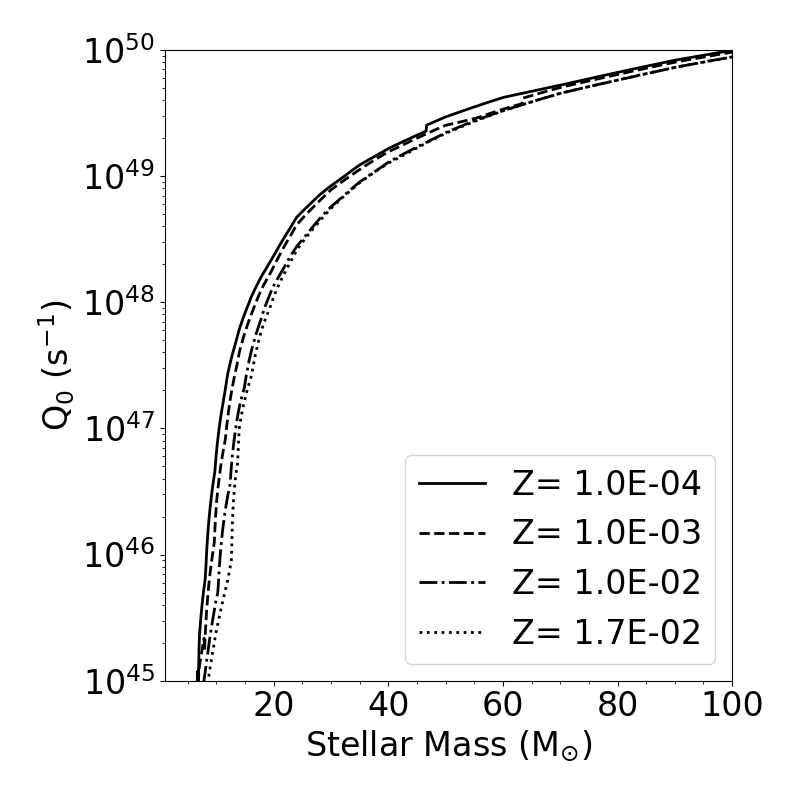
\includegraphics[width=0.4\linewidth]{figures/ch1/Q0}
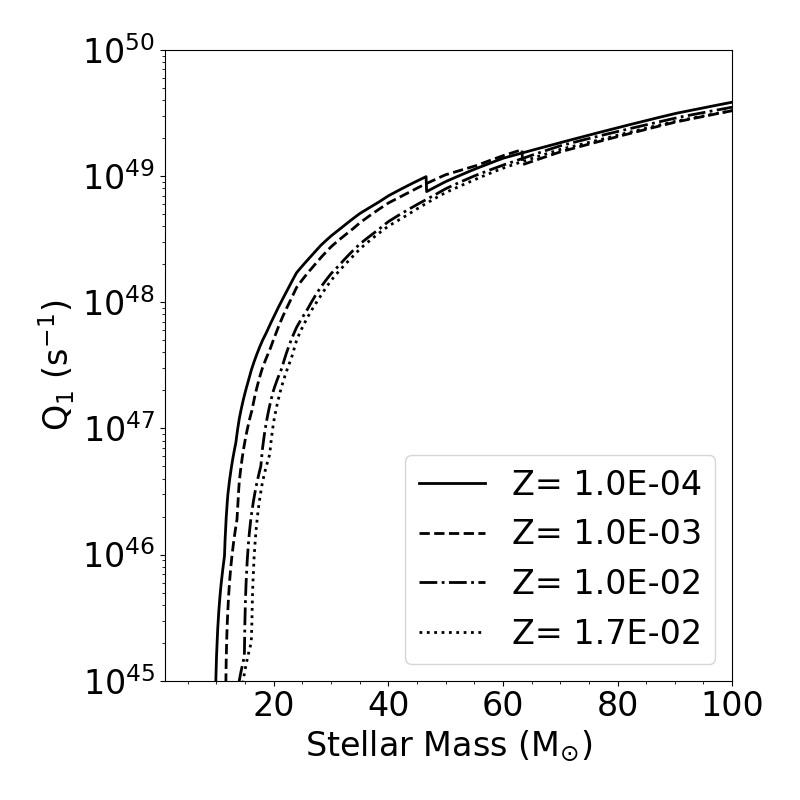
\includegraphics[width=0.4\linewidth]{figures/ch1/Q1}
\vspace{0.01cm}
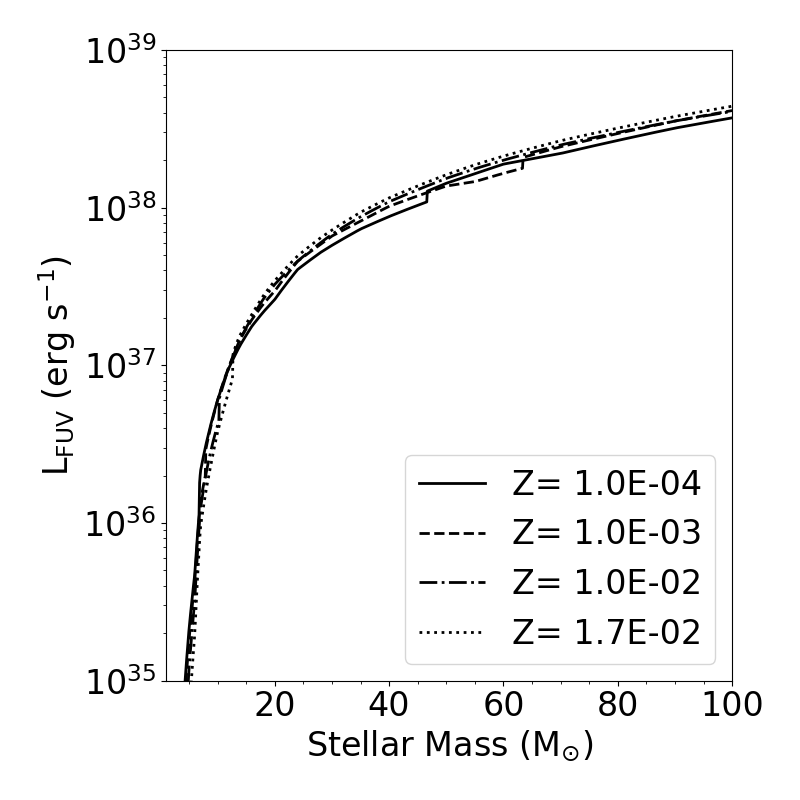
\includegraphics[width=0.4\linewidth]{figures/ch1/L_FUV}
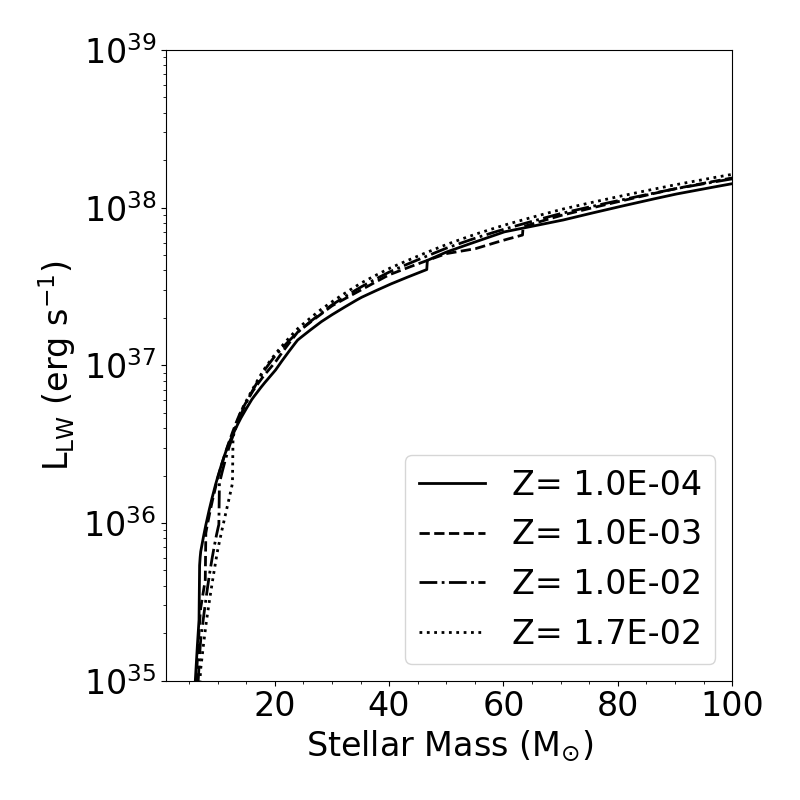
\includegraphics[width=0.4\linewidth]{figures/ch1/L_LW}
\vspace{0.01cm}
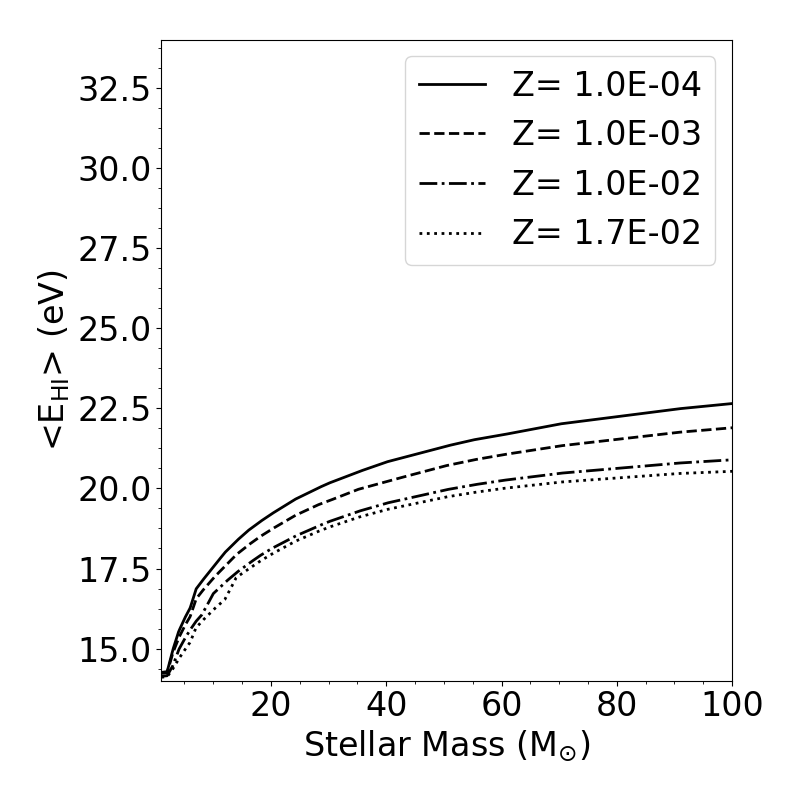
\includegraphics[width=0.4\linewidth]{figures/ch1/E0}
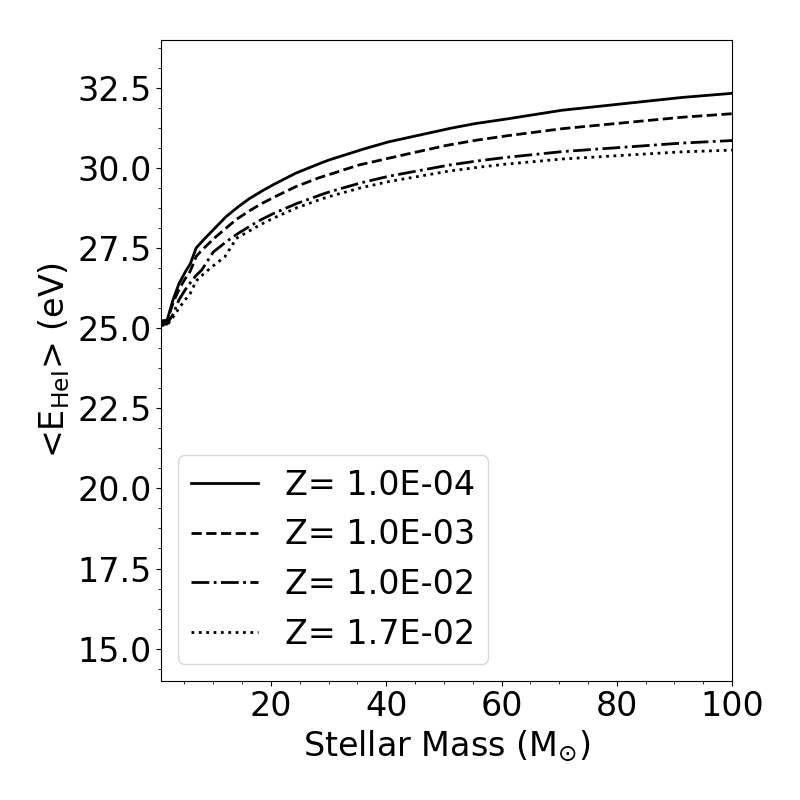
\includegraphics[width=0.4\linewidth]{figures/ch1/E1}
\caption{Radiation properties for our model stars, showing the ionizing photon luminosities for HI (top left) and HeI (top right) for each star, the FUV (middle left) and Lyman-Werner (middle right) luminosities, and finally the average ionizing photon energy for HI (bottom left) and HeI (bottom right). Note, we only track radiation from stars above 8.0 \msun, which dominate over less massive stars, even when accounting for IMF weighting.}
\label{fig:ch1:stellar radiation properties}
\end{figure*}

\setcounter{figure}{0}
\section{Typical Gas Densities in Supernova Injection Regions}
\label{appendix:SN}

Modeling SN feedback with the injection of thermal energy alone can lead to rapid overcooling of the injected energy, and a significant underestimate of the effects of SN feedback. Often, ad hoc solutions to this problem are used in large simulations with coarse resolution, such as momentarily turning off cooling in feedback affected regions or decoupling affected regions from the hydrodynamics for some time. However, physically consistent solutions have been developed \citep[e.g][]{Simpson2016} that inject a mixture of kinetic and thermal energy with a ratio that depends on resolution and local gas density. Overcooling becomes less important with higher resolution and lower ISM densities, until eventually pure thermal energy injection is sufficient to resolve each SN. We take advantage of our high resolution and employ a simple thermal energy injection model for our SN feedback. We demonstrate how well this resolves our SNe in the comparison simulation presented in this work.

The left panel of Fig.~\ref{fig:ch1:SN histogram} gives the distributions of the peak and average ISM number densities in the SN injection regions for each SN in our fiducial simulation. As shown, a majority explode in regions at substantially lower densities than the star formation threshold of 200~cm$^{-3}$. For most SNe, $n_{\rm max} \le 1.0$~cm$^{-3}$, which is due to the substantial pre-SN feedback included in our simulations. The right panel of Figure ~\ref{fig:ch1:SN histogram} gives the fractional distribution of the calculated radius of the pressure-driven snowplow ($R_{\rm PDS}$) phase of the Sedov-Taylor expansion, adopting the definitions from \citet{Simpson2016}
\begin{equation}
R_{\rm PDS} =
\begin{cases}
49.3E^{1/4}_{51}n^{-1/2}_{o} & if  Z \le 0.01 \\
18.5E^{2/7}_{51}n^{-3/7}_{o}Z^{-1/7} & if  Z \ge 0.01 \\
\end{cases}
\end{equation}
where $E_{51}$ is the injection energy in units of 10$^{51}$~erg, $n_{o}$ is the number density of the medium, and $Z$ is the metallicity in units of $Z_{o}$. \citet{Simpson2016} found that $R_{\rm PDS} > 4.5 \Delta x$ is needed to resolve the SN explosion with thermal energy injection alone, assuming uniform density in the injection region. In practice, the injection region is never uniform. We give $R_{\rm PDS}$ assuming uniform density at both the average and maximum number density in the injection region of each SN. As shown, a majority of SNe are resolved (to the right of the 4.5$\Delta x$ line), but up to 8.3\% are not well resolved and 2.0\% are completely unresolved (below a single cell width). In general, these are SN explosions from the most massive (i.e. most prompt) stars. We do not expect that resolving these SNe will dramatically alter our results. However, we note that using our feedback model at resolutions much less than a few parsecs will require implementing an different injection mechanism.

\begin{figure*}
\centering
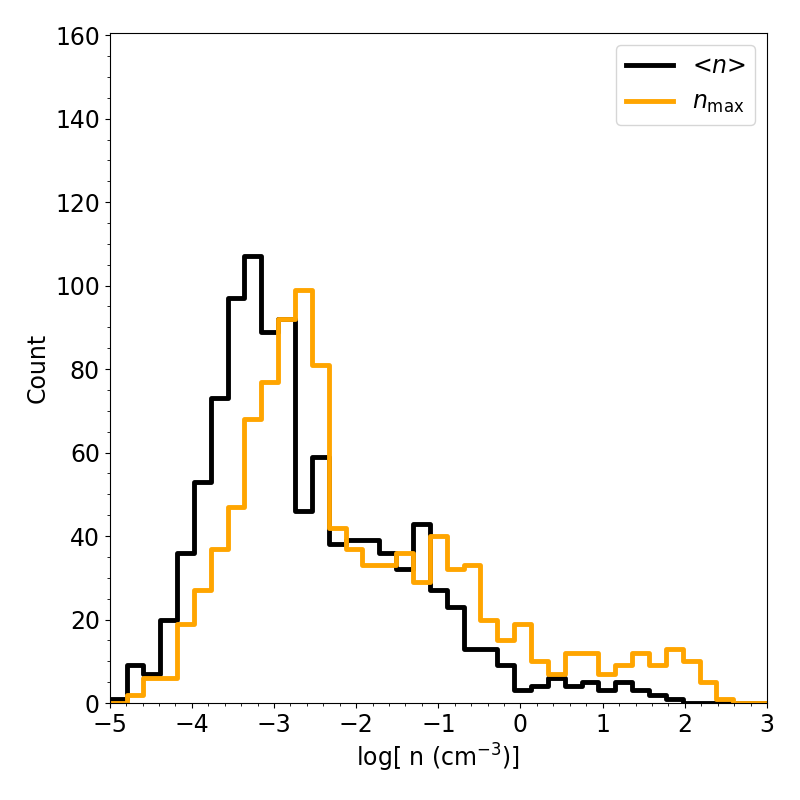
\includegraphics[width=0.4\linewidth]{figures/ch1/sn_density_hist}
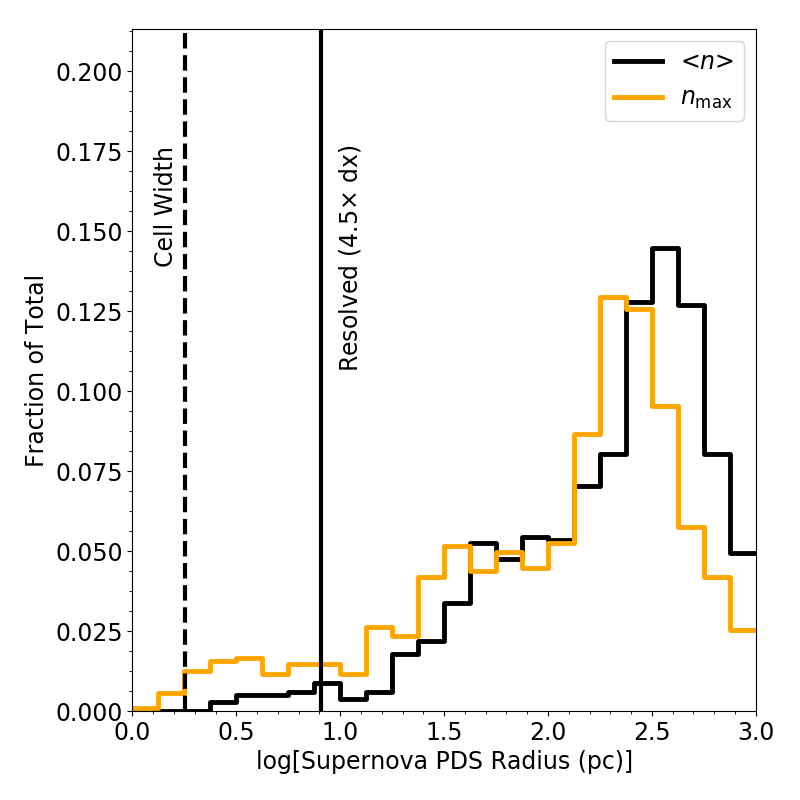
\includegraphics[width=0.4\linewidth]{figures/ch1/sn_radius_hist}
\caption{{\em Left:} Distribution of peak (orange) and average (black) gas densities in the injection region of each of the SNe from the simulation. {\em Right:} Distribution of the radius of the pressure-driven snowplow phase for each SN assuming a uniform medium at either the peak or average density in the injection region. The vertical lines show one and 4.5 cell widths. This shows that a fraction of these SNe are certainly unresolved, with R$_{\rm PDS}$ less than a single cell size, and somewhat more don't satisfy the 4.5 cell criterion, but the majority are well resolved.}
\label{fig:ch1:SN histogram}
\end{figure*}

\setcounter{figure}{0}
\section{Cooling and Heating Rates}
\label{appendix:cooling}

\begin{figure*}
\centering
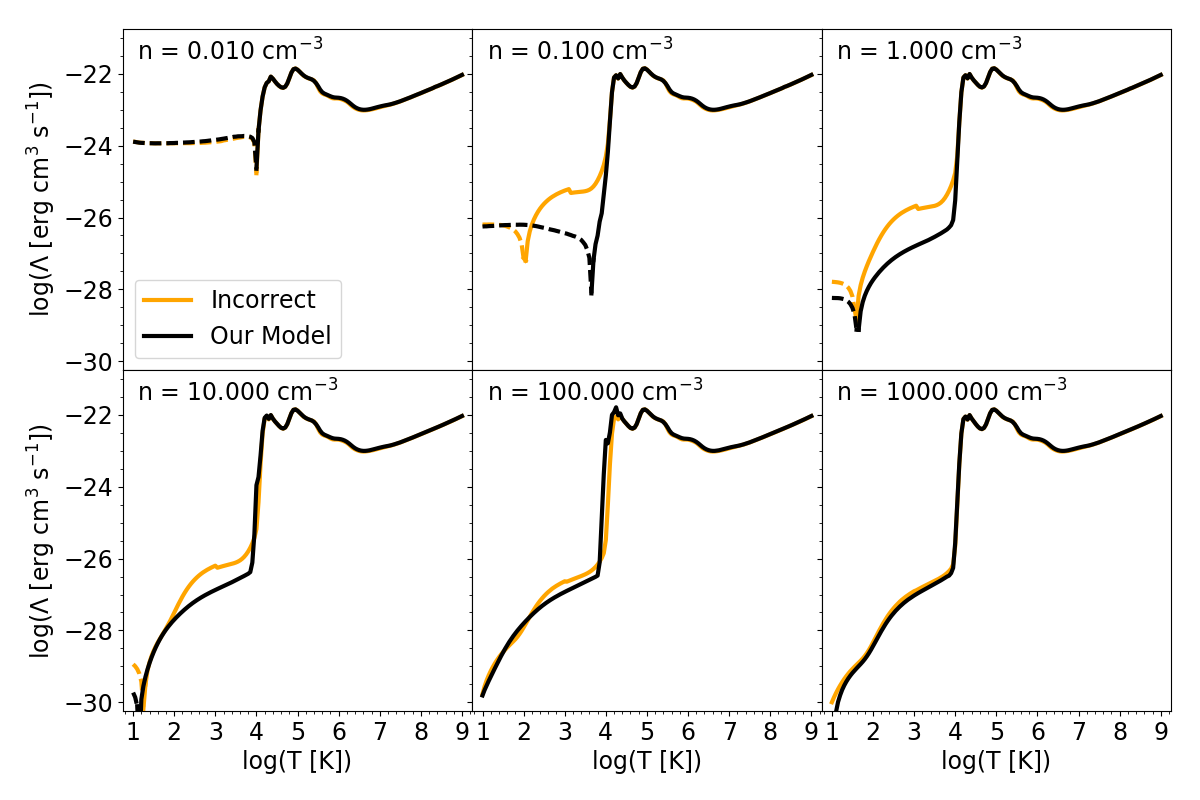
\includegraphics[width=0.95\linewidth]{figures/ch1/cooling_model_comparison}
\caption{The absolute value of the net cooling or heating rate in two models that account for self-shielding of primordial gas against a metagalactic UV background. Our model (black) uses self-consistent metal line cooling rates, and is compared to an incorrect model (orange) that adopts the uncorrected (i.e. optically thin) metal line cooling rates. The regimes where heating dominates are plotted with dashed lines for clarity.}
\label{fig:ch1:cooling comparison}
\end{figure*}


The cooling curves used in this work include a correction to a significant conceptual inconsistency one may encounter when using tabulated metal line cooling rates in combination with a self-shielding approximations. \citet{Hu2017} details this inconsistency: metal cooling rates computed under the assumption of an optically thin UV background overestimate the electron fraction in regimes where self-shielding is important ($-0.5 \leq \rm{log(n~[cm^{-3}])} < 2$). This results in an artificially enhanced metal line cooling rate in regions of self-shielding. This can be a significant effect, particularly at higher metallicities. We demonstrate this in Fig.~\ref{fig:ch1:cooling comparison}, which gives the absolute value of the net cooling rate for our full model at $Z = 0.1$~Z$_{\odot}$ (discussed below) as compared to a model using the optically thin metal line cooling rates at a range of densities. The effect is most significant at moderate densities, where the net cooling rate can be an order of magnitude higher. In low temperature regions, this can significantly shift the inferred equilibrium temperature and reduce the cooling time of dense gas. Fig.~\ref{fig:ch1:cooling} shows the net cooling rate and the individual heating and cooling rates from our generated tables at low metallicity, $Z = 0.01$~Z$_{\odot}$, comparable to that used in our dwarf galaxy. We have made these tables publicly available in the main distribution of \texttt{Grackle} and discuss how they were generated below.

For densities where self-shielding is important, we computed \textsc{Cloudy} models of one-dimensional clouds at each temperature and density pair with a physical size corresponding to the Jeans length. In cases where the Jeans length is very large, we limit the size to 100 pc, a reasonable approximation for the maximum size of a self-gravitating cloud. We then adopt the metal line cooling rates obtained from the center of these clouds, whose outside is exposed to the UV background. These models were computed with a modified version of the \texttt{CIAOLoop}\footnote{https://bitbucket.org/brittonsmith/cloudy\_cooling\_tools (our version: https://github.com/aemerick/cloudy\_tools)} code used in \citet{2008MNRAS.385.1443S}. In computing these tables we had to include the cosmic ray ionization that dominates in optically thick clouds. Without this effect, \textsc{Cloudy} becomes unstable in entirely neutral regions. We adopted a cosmic ray ionization rate of 10\% the Milky Way value, though we note that varying this from 1\% to 100\% the Milky Way value did not have an effect on the extracted metal line cooling rates.

Finally, we note that the cooling and heating rates in our simulation will deviate from these curves, as they depend upon local conditions that cannot be accounted for here. The primordial cooling and heating rates are computed consistently with the non-equilibrium chemistry solver, leading to deviations from the tabulated primordial rates, and the heating rates depend upon the local stellar radiation field, which is not included in these diagrams.


\begin{figure*}
\centering
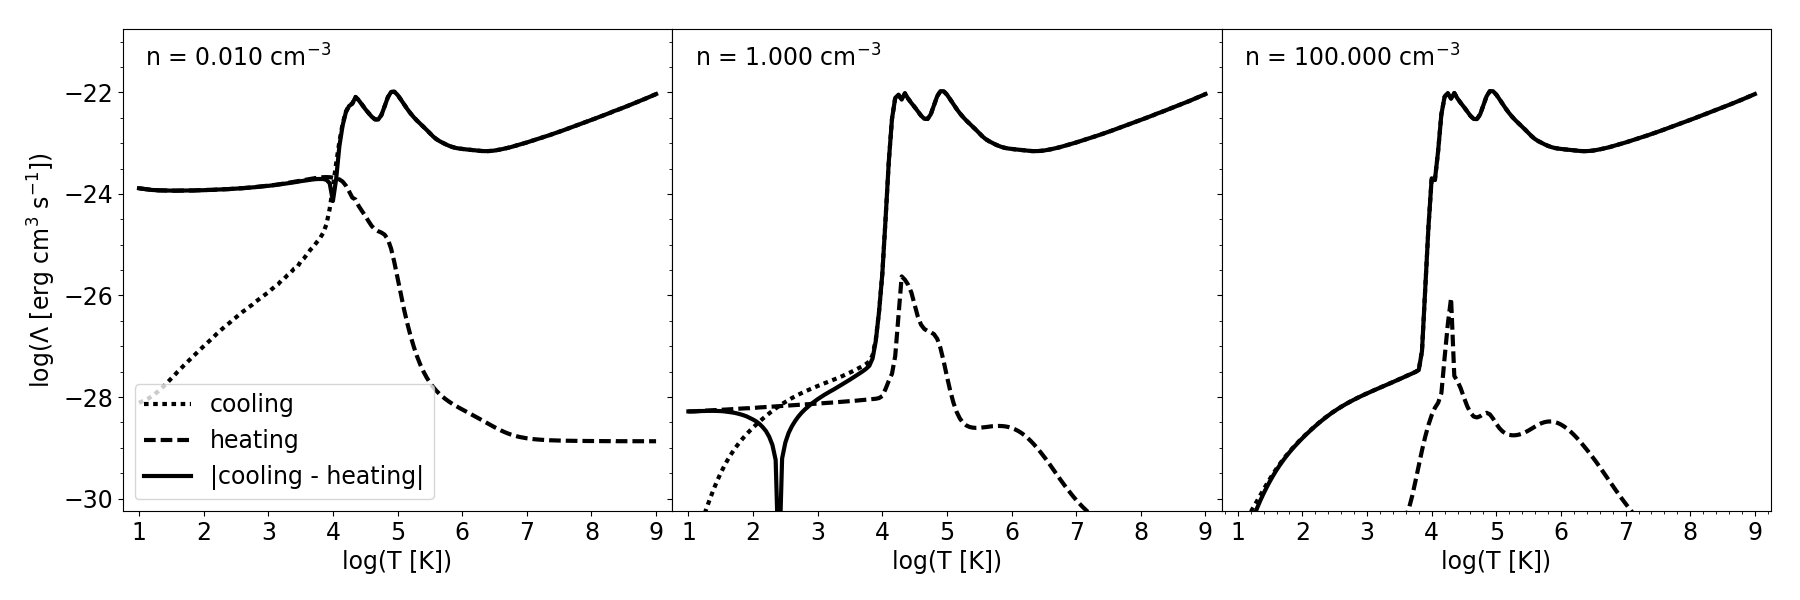
\includegraphics[width=0.95\linewidth]{figures/ch1/cooling_curve}
\caption{The total heating (dotted) and cooling (dashed) rates extracted from the core of a Jeans-length sized cloud irradiated by a \citet{HM2012} metagalactic UV background as modeled in \textsc{Cloudy}. The absolute value of the net cooling or heating
rate is shown with solid lines.}
\label{fig:ch1:cooling}
\end{figure*}

\setcounter{figure}{0}
\section{H$^{-}$ Photodetachment}
\label{appendix:H minus}

As discussed in Section~\ref{ch1:sec:molecular gas content}, H$_2$ formation is dominated by the gas-phase H$^{-}$ channel in our simulations. Accounting for the photodetachment of H$^{-}$ from the stellar radiation field, which may dominate over the UVB, can be important for correctly modeling H$_2$ formation in low metallicity gas~\citep{Wolcott-Green2012}. Our current model does not include this contribution. To test the significance of this radiation in determining the final H$_2$ mass we run a grid of one-zone Grackle cooling models.\footnote{See the ``cooling\_cell.py'' example here for more details: https://grackle.readthedocs.io/en/latest/Python.html}  These runs iterate through the non-equillibrium chemistry and cooling solvers with a constant density (10~cm$^{-3}$) and initial temperature of 10$^{4}$~K for 200~Myr. In Fig.~\ref{fig:ch1:Grackle grid} we plot the final H$_2$ mass fraction in these cells for variations over five orders of magnitude in the adopted H$^{-}$ photodetachment rate and the Lyman-Werner radiation background. As shown, the H$_2$ mass fraction is much more sensitive to the Lyman-Werner radiation field than the H$^-$ photodetachment rate. In effect, our simulations move left-to-right in this diagram (only) as stars form (right) or die (left). A complete model, including the stellar contribution to H$^{-}$ photodetachment, would move somewhat diagonally.

We follow up on the qualitative conclusions of these models by running four simulations at the four points in the diagram. These runs have identical initial conditions, random SN driving, cooling, heating, and chemistry as our fiducial simulation, but with no star formation. We vary the Lyman-Werner radiation and the H$^{-}$ photodetachment rate by the factors shown, which are comparable to the ratio between the typical ISRF and the UVB in the disk of our galaxy (see Fig.~\ref{fig:ch1:ISRF}). Changing the background H$^{-}$ photodetachment rate by a factor of 100 only (top left star) leads to a reduction in the final H$_2$ mass fraction by 3, while changing the Lyman-Werner background by a factor of 100 (bottom right point) decreases the H$_2$ mass by a factor of 6.9. Applying both scale factors gives a reduction of 7.9. Thus, we see that the difference between the more realistic case in which both rates increase by the same factor, and the case assumed in the simulations, is only about 20\%.

Although the replacement of star formation by random SNe in these models produces qualitatively different galaxy properties, the point of these simulations is to be maximal models of H$_2$ formation. We demonstrate that, even in this case, there is not a dramatic change in the total H$_2$ formation and that the effect of varying the H- photodetachment rate is sub-dominant to other factors. Therefore, we do not expect that ignoring this component of the stellar radiation field will have a significant dynamical impact on our galaxy evolution.

\begin{figure}
\centering
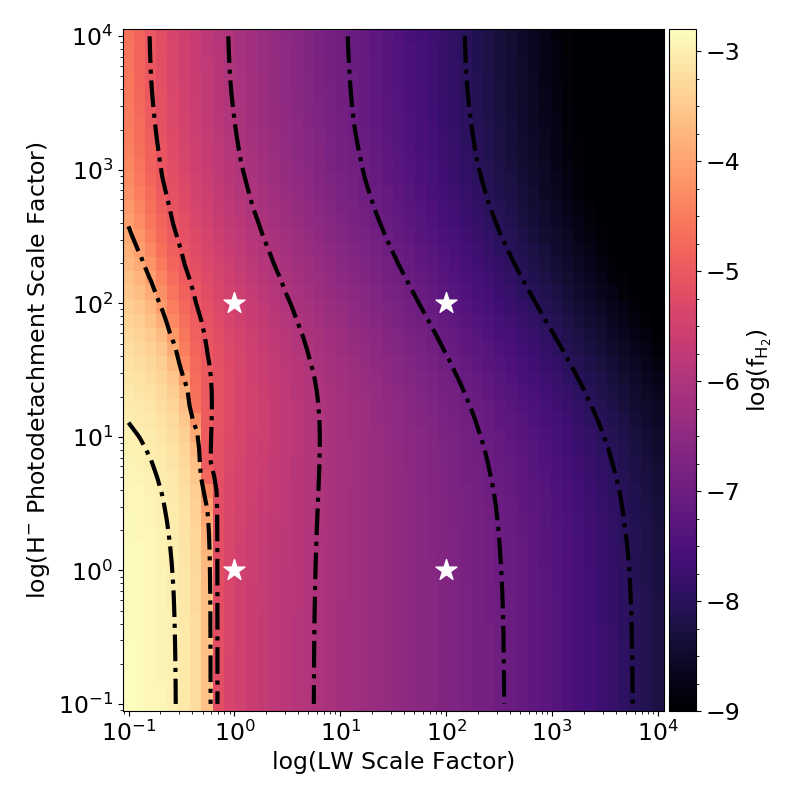
\includegraphics[width=0.95\linewidth]{figures/ch1/fH2.png}
\caption{The final H$_2$ mass fraction in a grid of one-zone Grackle cooling models run with the same Grackle parameters and metallicity as our full hydrodynamics simulation. Each model is held at a uniform density $n = 10$~cm$^{-3}$. Each model varies either the H$^{-}$ photodetachment rate or the Lyman-Werner background over their respective UVB values by a given scale factor. Contours give factors of ten change in the H$_2$ fraction. We note the regime below 1.0 on each axis is somewhat unphysical, and is never reached in our hydrodynamics simulations.}
\label{fig:ch1:Grackle grid}
\end{figure}

H$^-$ photodetachment arises from lower energy photons, above 0.76~eV, with a peak in effectiveness around 2~eV. For this reason, low mass stars may contribute significantly, if not dominate, the radiation field responsible for this reaction. The Lyman-Werner radiation field is dominated by short-lived massive stars, with some contribution from older stars up to a few hundred Myr, and is thus subject to significant fluctuations, particularly in periods of no star formation. During these times, H$^-$ photodetachment from low energy photons may play a non-negligible role in regulating H$_2$ formation. Indeed there is H$_2$ growth during these periods due to a decrease in the Lyman-Werner field, but it is unclear how much of this would be attenuated by accounting for photons from lower mass stars. Doing so in our current model, applying an optically thin $1/R^2$ field for each star, would be computationally challenging due to the dramatic increase in the number of stars whose radiation would need to be tracked.

As emphasized in Section~\ref{ch1:sec:molecular gas content}, further work modeling low-metallicity dwarf galaxies with a more detailed chemistry model would be useful to clarify the role of various competing phenomena in driving the molecular properties of these galaxies.

\setcounter{figure}{0}
\section{Resolution Study}
\label{appendix:resolution_study}

We demonstrate the effect of varying resolution in the evolution of our galaxy model in Fig.~\ref{fig:ch1:resolution_study}. We compare the star formation rate, mass evolution, and metal ejection / retention fractions between our fiducial high-resolution simulation (solid lines) with the same simulation at two lower maximum resolutions, 3.6~pc (dashed lines), and 7.2~pc (dash-dotted lines). The physics in each simulation remains the same with the exception of star formation, which employs a resolution-dependent density threshold. A factor of two decrease in resolution translates to a factor of four decrease in the star formation density threshold, from 200~cm$^{-3}$ in our fiducial runs, to 50~cm$^{-3}$ and 12.5~cm$^{-3}$ in our 3.6~pc and 7.2~pc resolution runs respectively. As a result, the time at which star formation first occurs varies between the simulations, but we again define t = 0 as the time of first star formation in each simulation.

\begin{figure*}
\centering
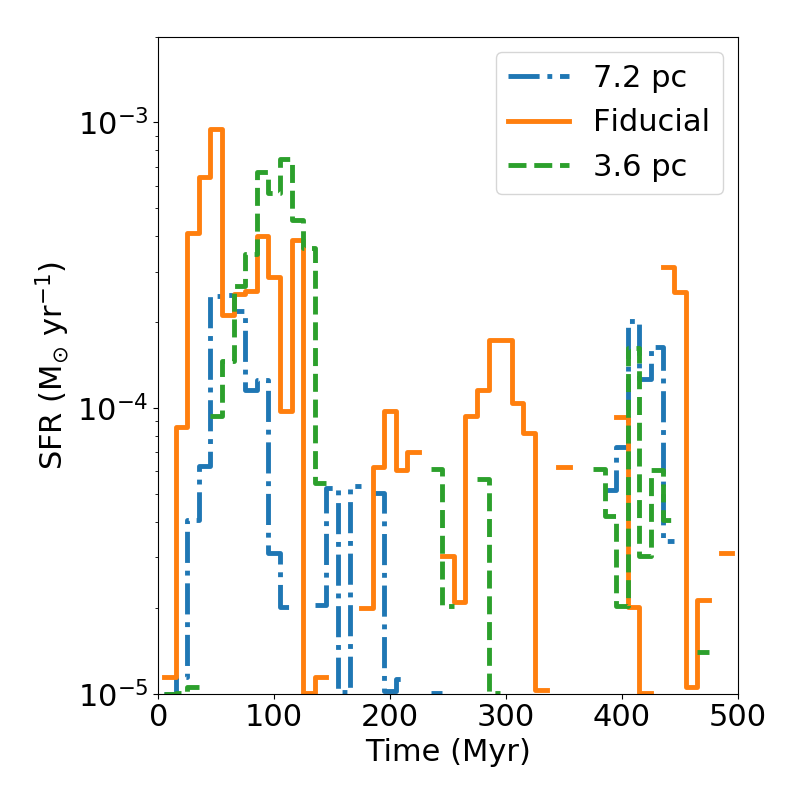
\includegraphics[width=0.33\linewidth]{figures/ch1/sfr_resolution_study.png}
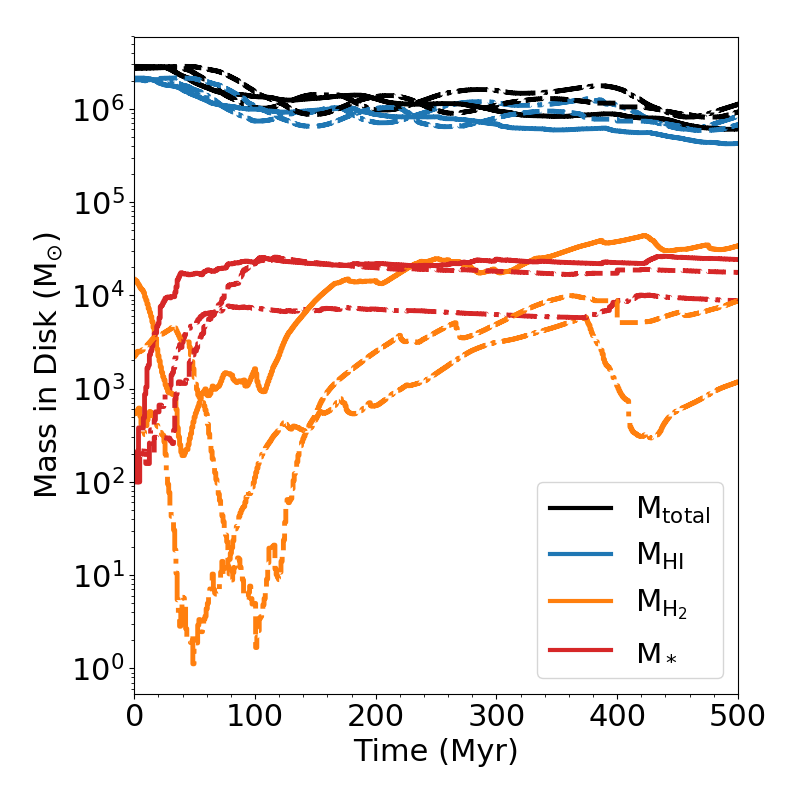
\includegraphics[width=0.33\linewidth]{figures/ch1/mass_evolution_resolution.png}
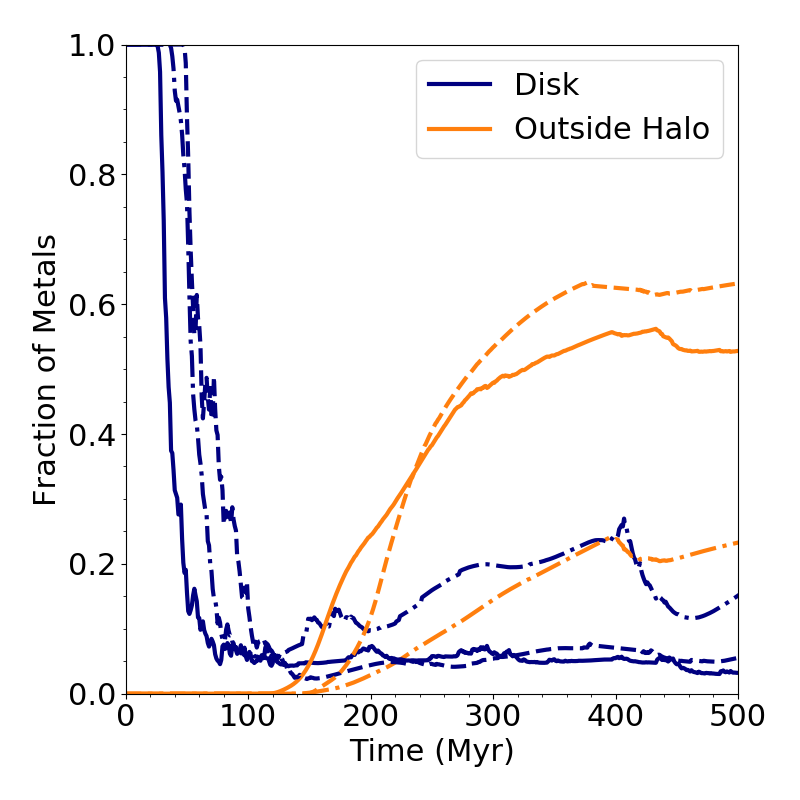
\includegraphics[width=0.33\linewidth]{figures/ch1/metal_retention_resolution.png}
\caption{A comparison of the SFR (left), disk gas mass (middle), and metal retention (right) evolution for our fiducial run (solid), 3.6~pc run (dotted), 3.6~pc run with a doubled initial supernova driving rate (dashed), and 7.2~pc run (dash-dotted). The line colors in the left panel are for better clarity between the SFRs.}
\label{fig:ch1:resolution_study}
\end{figure*}

Fig.~\ref{fig:ch1:resolution_study} shows that, while decreasing the resolution certainly changes the evolution, the simulations are similar to within a factor of a few. We argue that these differences are within the stochastic variation one would expect from simulations with stochastic star formation. The star formation rate and total stellar mass is correlated with resolution, with our fiducial run having the highest SFR and stellar mass among the three runs. We note that the self-consistent SNe are still resolved in the 3.6~pc runs since these still explode at the low densities seen in Fig.~\ref{fig:ch1:SN histogram}. However, although feedback in general is still effective in the 7.2~pc run, SNe are not well resolved at this resolution.

Generally ineffective feedback leads to increased, not decreased, star formation rates. However, the lower resolution run has the lowest SFR. The source of this difference is likely related to the ability to resolve dense, cold gas in the lower resolution simulations. In particular, the low resolution simulation clearly is unable to resolve the densities at which gas-phase H$_2$ formation becomes efficient, leading to significantly lower H$_2$ fractions (middle panel) and lower cooling rates. In addition, whatever H$_2$ does form at these lower resolutions exists at lower gas densities than in our fiducial run, and is less well protected by self-shielding effects. This is shown clearly in the significant plummet in the H$_2$ mass during the phase of first star formation that is less severe in our fiducial run. In this low metallicity regime, where H$_2$ is an important coolant, the ability to resolve the densities responsible for H$_2$ formation and self-shielding is important.

Theses differences in densities are shown clearly by comparing Fig.~\ref{fig:ch1:phase} with Fig.~\ref{fig:ch1:phase_resolution}. Although the lowest temperature reached in each simulation is comparable, there is less gas in the coldest, densest portion of the phase diagram in each of the lower resolution simulations. In the 7.2~pc run, the gas phases are notably less distinct, with gas more evenly smoothed out in the multi-phase region between cold, dense gas and warm, ionized gas. We note the 7.2~pc simulation, which ran quickly, was conducted without the temperature ceiling used in the 3.6~pc and fiducial runs; we do not expect this to have a significant effect on the comparison.


\begin{figure*}
\centering
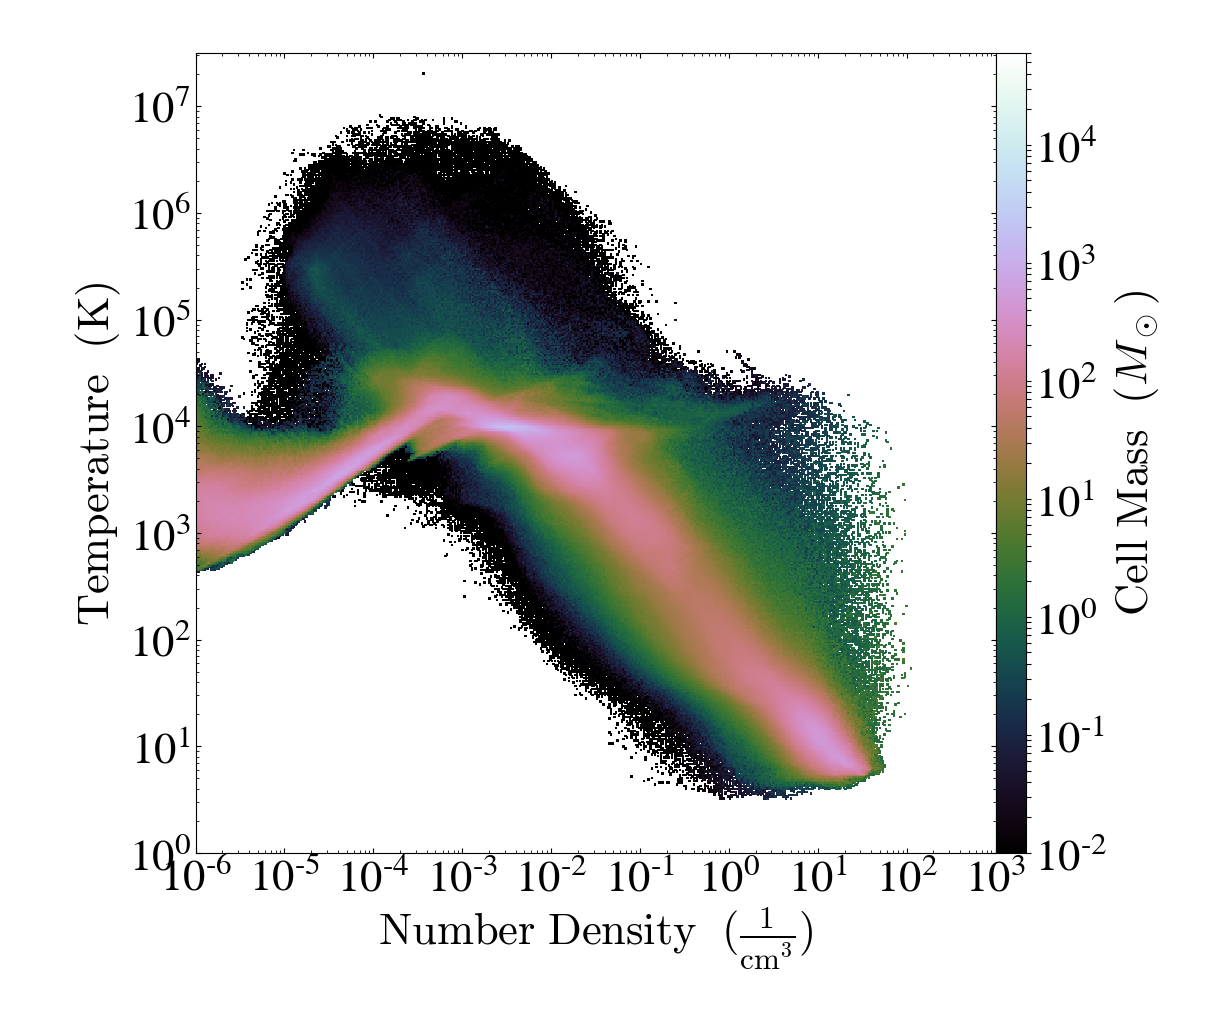
\includegraphics[width=0.475\linewidth]{figures/ch1/3pc_phase.png}
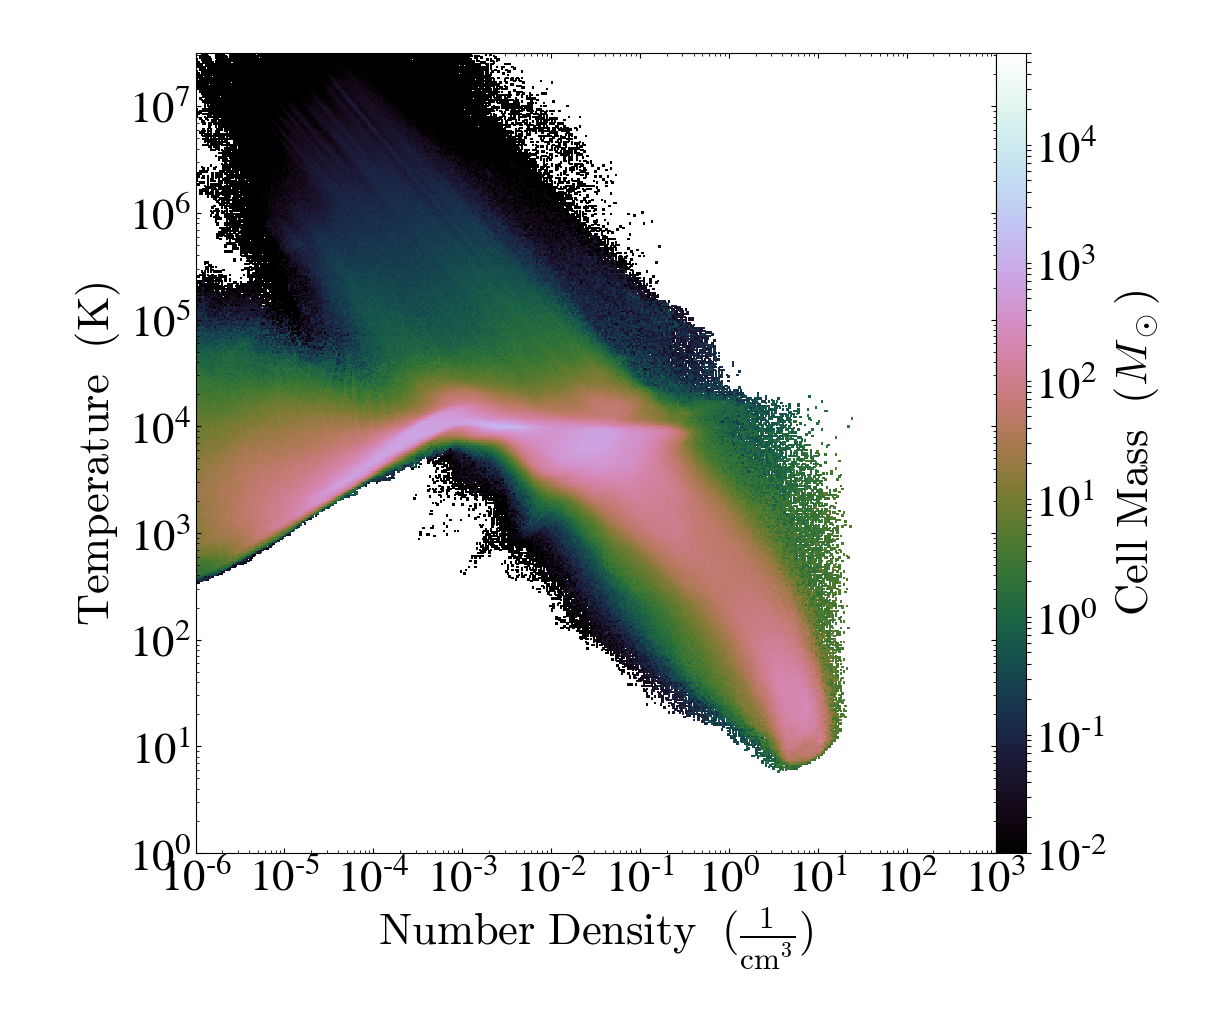
\includegraphics[width=0.475\linewidth]{figures/ch1/6pc_phase.png}
\caption{Temperature-density phase diagrams for our 3.6~pc run (left) and 7.2~pc run (right), as presented for our fiducial run in Fig.~\ref{fig:ch1:phase}.}
\label{fig:ch1:phase_resolution}
\end{figure*}

Finally, the metal retention fraction (right panel) between the fiducial and 3.6~pc runs are quite similar, but is significantly higher for the lowest resolution simulation. It is likely, however, that this is a result of the lower SFR in the 7.2~pc run and is not directly a resolution effect. This also affects the fraction of metals ejected outside the virial radius, with less metals being ejected in the lower resolution runs.

%\label{lastpage}


\renewcommand\thesection{\thechapter.\arabic{section}}

	\chapter[Stellar Radiation is Critical for Regulating Star Formation and Driving Outflows in Low Mass Dwarf Galaxies]{Stellar Radiation is Critical for Regulating Star Formation and Driving Outflows in Low Mass Dwarf Galaxies \label{ch:chapter2}}
\let\thefootnote\relax\footnotetext{This section contains text from an article published originally as \cite{Emerick2018a}}

%
% Copy paste paper here, without abstract or keywords
%
%\begin{abstract}
%
%Effective stellar feedback is used in models of galaxy formation to drive realistic galaxy evolution. Models typically include energy injection from supernovae as the dominant form of stellar feedback, often in some form of sub-grid recipe. However, it has been recently suggested that pre-SN feedback (stellar winds or radiation) is necessary in high-resolution simulations of galaxy evolution to properly regulate star formation and properties of the interstellar medium (ISM). Following these processes is computationally challenging, so many prescriptions model this feedback approximately, accounting for the local destruction of dense gas clouds around newly formed stars in lieu of a full radiative transfer calculation. In this work we examine high resolution simulations (1.8~pc) of an isolated dwarf galaxy with detailed stellar feedback tracked on a star-by-star basis. By following stellar ionizing radiation with an adaptive ray-tracing radiative transfer method, we test its importance in regulating star formation and driving outflows in this galaxy. We find that including ionizing radiation reduces the star formation rate (SFR) by over a factor of 5, and is necessary to produce the ISM conditions needed for supernovae to drive significant outflows. We find that a localized approximation for radiation feedback is sufficient to regulate the SFR on short timescales, but does not allow significant outflows. Short and long range radiation effects are both important in driving the evolution of our low-metallicity, low-mass dwarf galaxy. Generalizing these results to more massive galaxies would be a valuable avenue of future research.
%\end{abstract}

\section{Introduction} \label{ch2:sec:intro}
Historically, simulations of galaxy formation have suffered from the ``overcooling'' problem, whereby the action of self-gravity and radiative cooling alone produces galaxies with far too many stars. This problem has been addressed by employing various models of strong stellar feedback physics which are capable of generating self-regulating star formation in galaxies (see \cite{SomervilleDave2015} and \cite{NaabOstriker2017} for recent reviews). Energy injection from supernovae (SNe) has historically been used as the sole form of feedback. However, this is generally done heuristically as many simulations lack the ability to resolve the Sedov phase of individual SNe. But even with this strong feedback, recent work has argued for the need for pre-SN feedback, from stellar winds and/or stellar radiation \citep[e.g.][]{Hu2016,Hopkins2018}, though this is typically modeled simply as additional energy injection around newly formed stars. The need for additional feedback is confirmed by simulations that are capable of fully resolving individual SN \citep[e.g.][]{Peters2017,Smith2018a,Smith2018b,Hu2018}. However, modeling these processes in detail is challenging, and their competing effects on galactic evolution are poorly constrained.

Radiation from massive stars dominates the total feedback energy output of a stellar population \citep[e.g.][]{Abbott1982,Leitherer1999,Agertz2013}, surpassing the energy ejection of supernova ($\sim 10^{51}$~erg) by two orders of magnitude. If radiation couples effectively to the interstellar medium (ISM), it can be a substantial source of additional feedback. Simulations including stellar radiation feedback followed through radiative transfer or radiation-hydrodynamics schemes have found it to be effective in regulating star formation and driving galactic winds \citep[e.g.][]{WiseAbel2012,Kim2013a,Sales2014,Oshea2015,Rosdahl2015,Pawlik2015,Ocvirk2016,Peters2017}. This occurs in four ways: 1) heating of diffuse gas and preventing the formation of cold, dense star formation regions, 2) destruction of cold, dense gas around recently formed stars, preventing further star formation, 3) momentum input by direct absorption of UV radiation by gas and (in some cases) dust through re-emission and scattering in the infrared, and 4) lowering the typical ISM densities in which SNe occur and greatly increasing their effectiveness.

However, most works that employ stellar radiation feedback to account for these effects do so using various forms of sub-grid, approximate models to avoid the substantial additional cost of full radiative transfer. Many works use a Str{\"o}mgren approximation whereby the particles / cells within the Str{\"o}mgren radius around a radiating star are heated and kept ionized, with additional approximations made to account for overlapping ionized regions \citep[e.g.][]{HQM2011,Hu2016,Hu2017}. Other works employ some form of energy or momentum injection localized to the region immediately around a star particle \citep[e.g.][]{Agertz2013,Roskar2014,Ceverino2014,Forbes2016}. Although some of these approximate methods account for long-range effects of diffuse radiation \citep{HQM2012,Hopkins2018} most cases treat local radiation {\it only}, confined to energy or momentum injection in a limited physical region around a star particle. This is done both because the local destruction of dense clumps of gas around newly formed stars is commonly believed to be the dominant impact of stellar radiation feedback and because it is computationally less expensive to implement. The role of long-range stellar radiation, once ionizing photons break out of star forming regions, is not well characterized. Indeed it remains to be seen if modeling only the short-range effects of stellar radiation feedback is sufficient.

In this work we use a detailed model for stellar feedback presented in \cite{Emerick2019} (hereafter Paper I) to study the role of radiation feedback in dwarf galaxy evolution. For the first time in a galaxy-scale simulation, we resolve individual HII regions using an adaptive ray tracing radiative transfer method to follow the ionizing radiation from particles that represent individual stars. We focus on addressing two questions: 1) what role does radiation feedback play in regulating star formation, and 2) are the long-range effects of radiation feedback important, or is the local destruction of dense gas the dominant effect.

To investigate these questions, we compare three simulations of the evolution of an isolated, low mass dwarf galaxy. Our fiducial model, containing full stellar radiation feedback, is compared against a run without ionizing radiation feedback, and a run with ionizing feedback limited to the local region around a given star. We discuss our methods in Section~\ref{ch2:sec:methods} and present our results ion Section~\ref{ch2:sec:results}.

\section{Methods and Initial Conditions} \label{ch2:sec:methods}
We refer the reader to Paper I for a more detailed description of our methods. We use the adaptive mesh refinement hydrodynamics code \textsc{Enzo} \citep{Enzo2014} to evolve an idealized, isolated low mass dwarf galaxy. The galaxy is initialized as a smooth exponential disk set in hydrostatic equilibrium with a static dark matter potential \citep{Burkert1995} with $M_{\rm gas} = 2 \times 10^6~$~M$_{\odot}$, $Z_{\rm gas} = 4\times 10^{-4}$, radial and vertical gas scale heights of 250~pc and 100~pc respectively, and $M_{\rm vir} = 2.48 \times 10^9$~M$_{\odot}$, on a grid with a maximum physical resolution of 1.8~pc. We include no initial stellar population, but do include random driving from supernovae as an initial source of feedback up until the onset of star formation.

We include a UV background, tabulated metal line cooling, and a 9 species non-equilibrium chemistry solver using \textsc{Grackle} \citep{GrackleMethod}. Star formation occurs stochastically in cold, dense regions ($n > 200$~cm$^{-3}$, $T < 200$~K) by sampling a \cite{Salpeter1955} IMF from 1~M$_{\odot}$ to 100~M$_{\odot}$ and depositing \textit{individual} star particles over this mass range. We include feedback from stellar winds, AGB winds, FUV and LW band radiation which drives photoelectric heating and H$_2$ dissociation respectively, HI and HeI ionizing radiation, and core collapse and Type Ia SNe using thermal energy injection. FUV and LW band radiation are both taken to be optically thin, with local (cell-by-cell) attenuation alone. Ionizing radiation is followed using radiative transfer, as discussed below. Stellar lifetimes, surface gravity, effective temperature, and radii are set by the initial stellar mass and metallicity through interpolation over the PARSEC \citep{Bressan2012} zero age main sequence values. These properties are used to set the FUV, LW, and ionizing photon fluxes from each star through interpolation on the OSTAR2002 \citep{Lanz2003} grid. We only model the radiation from stars with masses above 8~M$_{\odot}$.

Our fiducial simulation follows photoionizing radiation using the adaptive ray-tracing radiative transfer method of \cite{WiseAbel2011}. This method places and evolves 48 rays on a HEALPix grid around each emitting source star for both HI and HeI ionizing radiation. Rays are adaptively split as they propagate away from their source to increase the angular resolution such that the solid angle of the ray remains smaller than 1/3 of the cell area. Rays begin on HEALPix refinement level 2, with a maximum refinement level of 13. We include radiation pressure on hydrogen, but do not investigate its importance in this work \citep[see][ and references therein]{Krumholz2018}.

We additionally present a simulation run without any stellar ionizing radiation (``noRT'') and a second simulation that includes ionizing radiation, but deletes all photons that travel more than 20~pc from their source (``shortrad''). This second simulation tests the relative importance of short-range vs. long-range effects of stellar ionizing radiation as a form of feedback. Although this is still more accurate than an approximate method, this is meant to function similarly to methods that include only the local effects of stellar radiation feedback. Each of our three simulations is identical up until the formation of the first star particles.\footnote{We note that the stars from the very first star formation event in each run (21 star particles with a total mass of 114 M$_{\odot}$) are the same. Of these, one particle emits ionizing radiation ($M_* > 8 $~M$_{\odot}$). The sampled stellar masses differ across runs after this point. Stochastic effects from differences in IMF sampling may be important in the regime of low mass, low SFR dwarf galaxies. Multiple re-simulations of identical initial conditions may result in significant scatter in their final properties \citep{Keller2018}. We find our main conclusions are likely to be insensitive to these stochastic variations, as we find that the total radiation output across multiple re-samplings of a fixed star formation history is small after the IMF is fully sampled.}

As shown in Paper I, the maximum densities reached in these simulations is below 10$^{3}$~cm$^{-3}$. Our inability to resolve the high densities in star forming regions ($\sim 10^5$~cm$^{-3}$) means that we likely underestimate initial photon absorption and overestimate the initial long-range effects of newly formed stars. However, in the Milky Way, newly formed O stars have been observed to spend no more than  10 -- 20\% of their main sequence lifetimes embedded in ultracompact HII regions within dense molecular clouds \citep{WoodChurchwell1989}. This short dispersal timescale agrees with high resolution simulations of massive star formation \citep[e.g.][]{Peters2010,Dale2014,Kim2018}. Therefore, we do not consider our neglect of this phase to be likely to lead to substantial errors at the galactic scale.

\section{Results} \label{ch2:sec:results}

\begin{figure*}
\centering
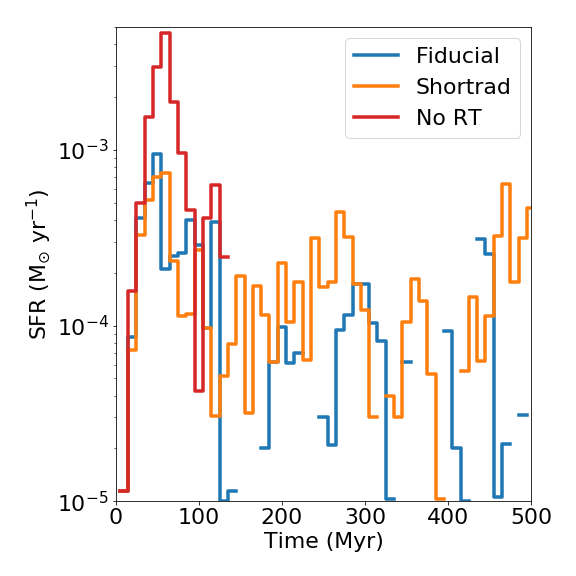
\includegraphics[width=0.49\linewidth]{figures/ch2/sfr}
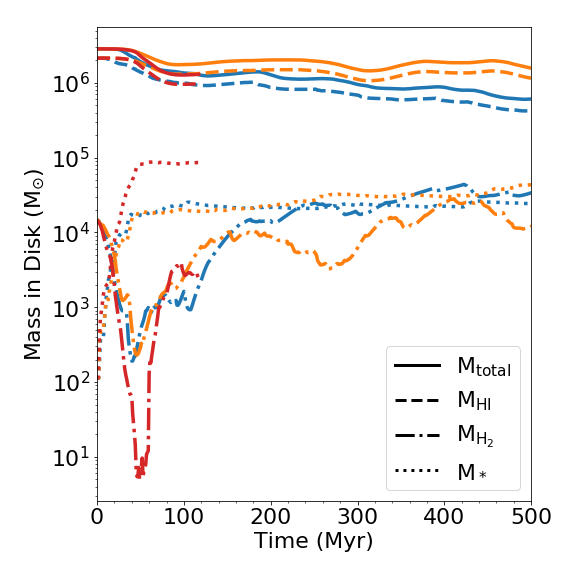
\includegraphics[width=0.49\linewidth]{figures/ch2/mass}
\caption{The star formation rate (left) and gas and stellar mass (right) of each of our three simulations over time. Time bins with no star formation are left empty.}
\label{ch2:figsfr_mass_evolution}
\end{figure*}

We compare the resulting star formation rate (left) and gas mass properties (right) of our three simulations in Figure~\ref{ch2:figsfr_mass_evolution}. There is a clear, significant contrast between the runs with and without ionizing radiation. Stellar ionizing radiation leads to a factor of $\sim$ 5 reduction in the resulting SFR, as compared to the noRT run. Since the shortrad and fiducial simulations are so similar over the first $\sim$~100~Myr, it is clear that stellar radiation acts to significantly reduce the local star formation efficiency around young, massive stars. Radiation from these stars quickly ionizes and dissipates surrounding dense gas that would otherwise have gone to fuel a significant amount of additional star formation. This is confirmed in Figure~\ref{ch2:figsf gas}, which shows the gas mass in each simulation above the SF density threshold of $n = 200$~cm$^{-3}$ during the first 100~Myr. While our fiducial and shortrad simulations remain roughly the same here, the noRT run, at its peak, has an order of magnitude more cold, dense gas. \footnote{We are unable to follow the long-term evolution of the noRT galaxy due to computational constraints. Although radiative transfer itself is computationally expensive, this run is substantially more costly due to a lower typical timestep and increased cost in computing the optically thin radiation effects (photoelectric effect and LW dissociation) for the additional star particles.}

\begin{figure}
\centering
\includegraphics[width=0.99\linewidth]{figures/ch2/mass_density_cut}
\caption{The total gas mass at $n > 200$~cm$^{-3}$, our star formation density threshold.}
\label{ch2:figsf gas}
\end{figure}

Looking again at the first $\sim$100~Myr of simulation time, the effects of ionizing radiation beyond our 20~pc cutoff radius are not significant. However, these two simulations begin to diverge after this point. The shortrad simulation has continual, steady star formation for the entire simulation time, while the star formation rate in our fiducial run is bursty, with periods of active, low-level star formation interspersed with periods of no star formation. The driver of these differences is clear in the right hand panel. Our fiducial run loses a factor of $\sim 2$ more total gas and HI mass (orange and blue lines) as compared to the shortrad simulation. Clearly, galactic winds and outflows are much more effective in with full accounting of stellar ionizing radiation feedback.

This can be confirmed by examining the metal retention fraction (the fraction of produced metals retained within the disk of the galaxy) and mass outflow rates across simulations. As shown in Figure~\ref{ch2:figmetal_retention}, the mass outflow rate in the fiducial run peaks at an order of magnitude higher at 0.25~R$_{\rm vir}$ than the shortrad simulation, declining only due to a comparative drop off in star formation. The outflow in noRT is only a factor of a few lower than the fiducial run, but it requires a five times higher supernova rate in this simulation to match the same outflow seen with full stellar radiation feedback, so it implies a far lower mass loading factor. Because of this difference in SFR,
%mm [rewrote to display equation]
the differences across simulations are more significant for our computed mass loading factor
\begin{equation}
    \eta = \frac{ \dot{M}_{\rm out}}{ <\rm{SFR}>_{100 \rm{Myr}}}.
\end{equation} The brackets indicate time averaging over 100~Myr.
%
While the fiducial run reaches a peak $\eta$ of a few hundred, shortrad is consistently an order of magnitude or more below this. The noRT simulation is even lower.

The fiducial run is also the only one of the three with any significant outflow beyond the virial radius. We conclude that radiation feedback allows SNe to be substantially more effective in driving outflows.

\begin{figure*}
\centering
\includegraphics[width=0.32\linewidth]{figures/ch2/metal_retention}
\includegraphics[width=0.32\linewidth]{figures/ch2/mass_outflow_comparison}
\includegraphics[width=0.32\linewidth]{figures/ch2/mass_loading_comparison}
\caption{{\bf Left:} The fraction of metals contained within the ISM of each galaxy (blue) and the fraction ejected beyond the virial radius (orange). As in Figure~\ref{ch2:figsfr_mass_evolution}, the fiducial run is given as solid lines, while the noRT and shortrad are dash-dotted and dashed respectively. {\bf Middle:} The mass outflow rate for each run at 0.25~R$_{\rm vir}$ (solid) and R$_{\rm vir}$ (dashed). {\bf Right:} The mass loading factor $\eta$ calculated as the outflow rate divided by the SFR averaged over 100~Myr. Inclusion of diffuse ionization makes an order of magnitude difference in $\eta$ in this case. }
\label{ch2:figmetal_retention}
\end{figure*}


\section{Discussion} \label{ch2:sec:discussion}
Accounting for feedback from stellar radiation plays a significant role in determining the ability for SN energy to couple to the ISM and therefore drive outflows. We believe this work is novel in examining the
importance of localized ionization vs.\ ionization from a diffuse radiation field far from a single star. Modeling only local stellar ionizing feedback is insufficient to describe the long-term evolution of an isolated dwarf galaxy. To explore the cause of this difference we compare in Figure~\ref{ch2:figpanel1} and~Figure~\ref{ch2:figpanel2} the gas number density (left), temperature (middle), and hydrogen ionization fraction (right) in edge-on slices in each of our simulations at two different times.

\begin{figure*}
\centering
\includegraphics[width=0.99\linewidth]{figures/ch2/DD0136_fiducial_shortrad_nort}
\caption{Edge-on slices of each simulation showing gas number density (left), temperature (middle), and hydrogen ionization fraction (right) 17~Myr after the formation of the first star in each run. Each panel is 4 kpc x 4 kpc. The full movie of this evolution from 0 to 118 Myr is included for further clarification. This movie demonstrates that the differences in outflows between the simulations depends on the ability for feedback to carve low-density, ionized channels along which SNe can launch gas beyond the disk of the galaxy. These channels are readily created by ionizing radiation in the fiducial simulation, or to some degree by SNe in the noRT simulation due to its much higher SN rate. However, SNe launched gas is trapped by neutral, cold shells in the shortrad simulation, unable to easily escape from the disk of the simulated galaxy. These same insights can also be gained by comparing this figure with Figure~\ref{ch2:figpanel2}.}
\label{ch2:figpanel1}
\end{figure*}

\begin{figure*}
\centering
\includegraphics[width=0.99\linewidth]{figures/ch2/DD0160_fiducial_shortrad_nort}
\caption{Same as Figure~\ref{ch2:figpanel1}, but at 40~Myr.}
\label{ch2:figpanel2}
\end{figure*}

Figure~\ref{ch2:figpanel1}, at 17~Myr, compares each simulation just after the first few SNe. Already there are significant differences between the runs. Gas outside the galaxy is warm ($\sim$~10$^{4}$~K) and ionized up to $\sim$500~pc above/below the plane of the disk in our fiducial run. This same gas is cold ($<10^4$~K) and neutral in both other runs. The contrast between the effect of ionizing radiation in the fiducial and shortrad runs is seen most clearly in the ionized region in-plane and to the right of center. This region contains massive stars that are capable of generating enough ionizing radiation to carve a channel out to the halo of our fiducial simulation; this does not occur in the shortrad case. Instead, the HII region is confined by surrounding cold, neutral gas.

Although the ISM properties within the HII region in each case are quite similar between the simulations, the SNe that eventually go off in this region are confined by the neutral gas in the shortrad simulation, but readily escape through the lower density ionized gas into the galaxy halo in our fiducial case. As these simulations evolve, the existence of these diffuse, ionized channels in the fiducial run easily allow continual and significant outflows from SNe, as shown in  Figure~\ref{ch2:figpanel2}, which shows each simulation 40~Myr after the formation of the first stars. In contrast, the same SNe in the other two simulations are well contained, surrounded by shells of denser, neutral gas. Though they make an important local impact on the ISM, they are unable to drive significant mass loss from the galaxy. In the noRT case, an outflow does eventually develop, but it takes a factor of five increase in SFR, and a corresponding increase in supernova rate, for SNe to finally break out from the neutral gas surrounding the galaxy.

As shown in Figure~\ref{ch2:figmetal_retention} the differences in ionization structure and its effect on galactic winds has direct consequences for the chemical evolution of our dwarf galaxy. The winds in our fiducial simulation carry nearly all of the metals produced out from the disk of our galaxy. This is the only run in agreement with observations of Local Group dwarf galaxies, both dSph's \citep{Kirby2011} and the gaseous, star forming Local Group dwarf galaxy Leo P \citep{McQuinn2015}, with metal ejection fractions of up to 95\%. This is in stark contrast to the $\sim$30\% retention fraction in our shortrad simulation. This would also influence the chemical enrichment of neighboring galaxies, given the significant differences in metal ejection past the virial radius between these two runs. Clearly the effects of feedback on observable chemical properties of galaxies is a key discriminator among models.

These results show that long-range ionization effects are an important consideration in models of stellar feedback. However,
further study is warranted of how this effect can be approximated without resorting to full radiative transfer calculations. Approximate, Str{\"o}mgren-like feedback models that allow for ionization far from a single source \citep[e.g.][]{Hopkins2018} may be sufficient to capture the effects shown here. Fully localized methods, or methods which set a maximum for the ionization radius may underestimate galactic wind properties in dwarf galaxies. In addition, both methods are mass biased \citep[see the discussion in ][]{Hu2017}, preferentially over-ionizing dense gas that would otherwise be missed by photons leaking through channels carved through lower-density gas. These remaining uncertainties motivate a continued examination of the feedback prescriptions adopted in high resolution simulations of galaxy evolution.

\section{Conclusion}  \label{ch2:sec:conclusion}
In agreement with previous work we find that (local) stellar radiation feedback is effective in regulating star formation, but that non-local ionizing radiation is key for driving outflows in our simulations of an isolated, low mass, dwarf galaxy. Simulations run without ionizing radiation feedback have star formation rates a factor of five higher than our fiducial simulation. Despite the lower rate, SNe in our fiducial run are capable of driving larger galactic outflows, aided significantly by the ionizing radiation feedback.

We demonstrate for the first time that simple prescriptions of local stellar radiation feedback fail to reproduce the evolution of our fiducial model. Our simulation with radiation localized to 20~pc around each star particle does effectively regulate star formation on short time scales, predominately by quickly destroying cold, dense gas around young, hot stars. However, this model does not drive the significant outflows seen in our fiducial simulation. Long-range ionizing radiation is important for carving channels allowing the ejection of significant amounts of mass and metals from the SNe. Our simulation with localized radiation feedback retains a significantly higher fraction of metals than expected observationally for low mass dwarf galaxies.

Finally, we note that we have performed this experiment on only one possible type of galaxy. Its low virial temperature ($\sim10^{4}$~K) makes this galaxy particularly sensitive to the effects of stellar feedback, and ionizing radiation in particular. Examining the role of long-range, diffuse stellar ionizing radiation on star formation and galactic winds in more massive galaxies is an important avenue of future research.

\section*{Acknowledgments:}
A.E. is funded by the NSF Graduate Research Fellowship DGE 16-44869. G.L.B. acknowledges support from NSF AST-1312888, NASA NNX15AB20G, and NSF AST-1615955. M.-M.M.L. was partly funded by NASA  grant NNX14AP27G and NSF grant AST18-15461. We gratefully recognize computational resources provided by NSF XSEDE through grant number TGMCA99S024, the NASA High-End Computing Program through the NASA Advanced Supercomputing Division at Ames Research Center, Columbia University, and the Flatiron Institute. This work made significant use of many open source software packages, including \textsc{yt}, \textsc{Enzo}, \textsc{Grackle}, \textsc{Python}, \textsc{IPython}, \textsc{NumPy}, \textsc{SciPy}, \textsc{Matplotlib}, \textsc{HDF5}, \textsc{h5py}, \textsc{Astropy}, \textsc{Cloudy} and \textsc{deepdish}. These are products of collaborative effort by many independent developers from numerous institutions around the world. Their commitment to open science has helped make this work possible.

%\software{astropy \citep{astropy} matplotlib \citep{matplotlib}, Numpy \citep{numpy}, SciPy \citep{scipy}, IPython \citep{Ipython}, yt \citep{yt}, Enzo \citep{Enzo2014}, Grackle \citep{GrackleMethod}, CLOUDY \citep{cloudy}, HDF5 \citep{HDF5}}



%************* APPENDICES ************************%

%\clearpage
%\appendix
\setcounter{section}{0}%
\renewcommand\thesection{\thechapter.\Alph{section}}



\renewcommand\thesection{\thechapter.\arabic{section}}

	\chapter[Metal Mixing and Ejection in Dwarf Galaxies is Dependent on Nucleosynthetic Source]{Metal Mixing and Ejection in Dwarf Galaxies is Dependent on Nucleosynthetic Source \label{ch:chapter3}}
\let\thefootnote\relax\footnotetext{This section contains text from an article published originally as \cite{Emerick2018b}}

%
% Copy paste paper here, without abstract or keywords
%

%\begin{abstract}
%Using a high resolution simulation of an isolated dwarf galaxy, accounting for multi-channel
%stellar feedback and chemical evolution on a star-by-star basis, we investigate how each of 15 metal species are distributed within our multi-phase interstellar medium (ISM) and ejected from our galaxy by galactic winds. For the first time, we demonstrate that the mass fraction probability distribution functions (PDFs) of individual metal species in the ISM are well described by a piecewise log-normal and power-law distribution. The PDF properties vary within each ISM phase. Hot gas is dominated by recent enrichment, with a significant power-law tail to high metal fractions, while cold gas is predominately log-normal. In addition, elements dominated by asymptotic giant branch (AGB) wind enrichment (e.g. N and Ba) mix less efficiently than elements dominated by supernova enrichment (e.g. $\alpha$ elements and Fe). This result is driven by the differences in source energetics and source locations, particularly the higher chance compared to massive stars for AGB stars to eject material into cold gas. Nearly all of the produced metals are ejected from the galaxy (only 4\% are retained), but over 20\% of metals dominated by AGB enrichment are retained. In dwarf galaxies, therefore, elements synthesized predominately through AGB winds should be both overabundant and have a larger spread compared to elements synthesized in either core collapse or Type Ia supernovae. We discuss the observational implications of these results, their potential use in developing improved models of galactic chemical evolution, and their generalization to more massive galaxies.
%\end{abstract}

%\section*{Acknowledgments}

\section{Introduction}
Understanding galactic chemical evolution for all metal species across galaxy mass scales remains one of the most challenging aspects of modeling galaxy evolution. One of the most pressing difficulties is a lack of understanding in exactly how metals propagate from their injection sites from stellar winds or supernovae (SNe) and mix through the phases of the interstellar medium (ISM) into star-forming gas.

One-zone chemical evolution models assume homoegeneous mixing of metals from recent star formation into gas available for future star formation \citep[e.g.][]{Lanfranchi2006b,Kirby2011-III,Cote2017a,Andrews2017}. While this assumes that metal mixing in the ISM plays no role in delaying future enrichment in star formation, accounting for this process is challenging. More complex models \citep[e.g.][]{SchonrichBinney2009,Pezzulli2016} employ multiple (usually radial) zones or follow multiple gas phases to attempt to account for these effects. How to properly account for multi-phase mixing, however, is still poorly understood. This is in large part because both these models and large-scale cosmological simulations lack the necessary fidelity to capture the detailed, multi-phase mixing process of metals in the ISM directly. Recent hydrodynamics simulations have employed parametric models to account for unresolved sub-grid metal mixing \citep{PanScannapiecoScalo2013,Sarmento2017,Sarmento2018}, which plays an important role in determining the chemical properties of galaxies \citep[e.g.][]{Shen2010, Pilkington2012, Few2012, Brook2014, FengKrumholz2014, Armillotta2018, Escala2018, Rennehan2018} 
% KVJ: citations to high-redshift work in this area
%\textbf{
and the enrichment process and chemical signatures of the first stars \citep[e.g.][]{Jeon2015,Ritter2015,Smith2015}.
%}
Detailed hydrodynamics simulations incorporating a multi-phase ISM and detailed stellar feedback are required to understand the details of metal mixing and metal outflows in galaxies.

In addition, it remains to be seen to what degree, if at all, metals of different enrichment origins (AGB winds, core collapse SNe, Type Ia SNe, neutron-star neutron-star mergers, etc.) may couple differently to the ISM. When metals are tracked individually, as opposed to a global metallicity field, their injection, mixing, and outflow properties are often treated uniformly. However, if metals do not behave uniformly in the ISM, if their mixing and ejection behavior depends directly upon the energetics and physical environment of their injection, then this assumption would need to be re-evaluated. Differences in metal distributions from ejecta in AGB stars, as compared to SNe, has been explored recently in \cite{KrumholzTing2018}, but has yet to be demonstrated in hydrodynamics simulations. Relaxing this assumption has implications for both interpreting observations of stellar abundances in nearby dwarf galaxies and in modeling galactic chemical evolution in both semi-analytic models and lower resolution cosmological simulations \citep[e.g.][]{Cote2018}.

The use of low mass dwarf galaxies, both observationally in the Local Group and in theoretical models, has been critical in improving our understanding of galactic chemical evolution. That dwarf galaxies efficiently pollute the circumgalactic medium and intergalactic medium (IGM) with metals has been demonstrated for some time both theoretically \citep[e.g.][]{DekelSilk1986,MacLowFerrara1999,Fragile2004,Muratov2017,Corlies2018}, and with direct observational evidence from the metal retention fractions of Local Group dwarf galaxies \citep[e.g.][]{Kirby2011-metals,Bordoloi2014,McQuinn2015}. If there are differences in metal coupling to the ISM, this could potentially impact how metals are driven out of galaxies through galactic winds. This has implications for both interpreting observations of stellar abundances in nearby dwarf galaxies and in modeling galactic chemical evolution in both semi-analytic models and lower resolution cosmological simulations. However, examining this process has only become possible recently as it requires high resolution, galaxy-scale hydrodynamics simulations that can resolve ISM mixing and self-consistently drive galactic winds through multi-channel stellar feedback.
%It is commonly assumed that all metals couple equally to galactic outflows, however, which may not be a valid assumption if metals of different nucleosynthetic origins couple differently to the ISM \citep{KrumholzTing2018}. 
% Relaxing this assumption has implications for both interpreting observations of stellar abundances in nearby dwarf galaxies and in modeling galactic chemical evolution in both semi-analytic models and lower resolution cosmological simulations. However, testing this assumption has only become possible recently as it requires high resolution, galaxy-scale hydrodynamics simulations that can resolve ISM mixing and self-consistently drive galactic winds through multi-channel stellar feedback.

It is becoming increasingly valuable to develop a concrete theoretical understanding of galactic chemical evolution as a result of multiple, recent observational campaigns to probe detailed stellar abundances in our Milky Way and the Local Group, such as SEGUE \citep{Yanny2009}, RAVE \citep{Kunder2017}, APOGEE \citep{Anders2014}, and GALAH \citep{Buder2018}. Stellar abundances are directly imprinted with the enrichment pattern of their star-forming cloud, whose chemical properties are determined by the process of turbulent metal mixing in the ISM. The degree to which we can associate "chemically tagged" stars as co-eval depends directly upon our understanding of metal enrichment and metal mixing in the ISM. Furthermore, this understanding is critical for using these observations to further deduce properties of a galaxy's evolutionary history. 
% KVJ asked to bring up this area of research and emphasize how it is lacking theoretical input
%\textbf{

One key aspect of this work has been a significant effort to characterize the number of independent dimensions accessible by the multi-dimensional chemical abundances observed in these studies \citep[e.g][]{Freeman2002,Ting2012, Hogg2016,Jofre2017,Price-Jones2018}. Thus far, these studies have remained uninformed by hydrodynamics simulations and, conversely, these results cannot yet be used to constrain simulations. Doing so requires the kinds of high resolution, galaxy-scale multi-element chemodynamical simulations that have only become feasible in recent years. Recent work has suggested that low-mass dwarf galaxies are perhaps the best regime to begin understanding these processes \citep[e.g.][]{Bland-Hawthorn2010a,Bland-Hawthorn2010b,Karlsson2012,Webster2016}. This is advantageous, as their small physical size and low star formation rates makes conducting high resolution, hydrodynamics simulations of these systems computationally feasible.

In this paper we present the first detailed chemical evolution results from a set of high-resolution hydrodynamics simulations of an isolated, low-mass, dwarf galaxy performed with the adaptive mesh refinement code \textsc{Enzo} \citep{Enzo2014}. The simulation discussed here was introduced in detail in \cite{Emerick2019} (hereafter Paper I). To address the outstanding questions discussed above, these simulations follow star formation using individual star particles, including stellar feedback from massive star and AGB-phase stellar winds, photoelectric heating, Lyman Werner dissociation, ionizing radiation tracked through an adaptive ray-tracing radiative transfer method, and core collapse and Type Ia SNe. This is in addition to a detailed model for ISM physics using the \textsc{Grackle} library, as discussed below. We show that metals are strongly ejected via galactic winds, but that the retention of metals in the ISM and their mixing through phases varies significantly depending on the production source of the given elemental species. We show how these elements are distributed in the ISM and conclude with a discussion on the implications of these results.

The physical processes that drive galactic chemical evolution are complex, driven by the details of stellar feedback, turbulence and diffusion in a multi-phase ISM, and variations in stellar yields with nucleosynthetic source and stellar metallicity. Uncertainties in each of these processes make reproducing and interpreting observations of gas and stellar abundances challenging. 
%[list examples of modeling problems]. 
These uncertainties, combined with the difficulty in simulating a fully self-consistent galaxy in detail, motivates this current study. By focusing on a low mass dwarf galaxy, with small size and low star formation rate, we can capture detailed feedback and ISM physics at high resolution, while following individual stars. In this work we focus on theoretical quantities, namely the probability density distributions (PDFs) of metals in the ISM as a function of metal mass fraction, rather than the common observables of stellar and gas abundance ratios, for two reasons. First, we would like to build our understanding of galactic chemical evolution from a fundamental level. Second, there is only a limited sample of gas-rich, star forming dwarf galaxies of this size that we can use for direct observational comparison, and it is computationally infeasible to simulate galaxies of easily observable size in as much detail as done here. This work will be the first of several attempting to bridge this gap. With a more fundamental understanding of metal mixing and stellar enrichment in galaxies, we can construct better one-zone chemical evolution models and physically motivated sub-grid physics models for lower resolution simulations of more massive galaxies.

We summarize our methods and physics models in Section~\ref{sec:methods}. We begin our analysis by presenting the only direct observable comparison we can make at this galaxy mass, discussing the metal retention fractions of our galaxy in Section~\ref{sec:ejection}. In Section~\ref{sec:log-normal} we focus on how each of our 15 individual metal species are distributed and evolve within each phase of the ISM. We discuss our results in Section~\ref{sec:discussion}, and conclude in Section~\ref{sec:conclusions}.

% AE: Benoit suggested subsections instead of paragraph splits... play with this to see what looks best
\section{Methods}
\label{sec:methods}
We refer the reader to Paper I for a detailed description of our numerical methods and feedback models. We briefly summarize the relevant details here.

\paragraph{Hydrodynamics} We use the adaptive mesh refinement astrophysical hydrodynamics and N-body code \textsc{Enzo}\footnote{http://enzo-project.org/} \citep{Enzo2014}. Hydrodynamics are solved using a direct-Eulerian piecewise parabolic method and a two-shock approximate Riemann solver with progressive fallback to more diffusive solvers. We include gas self-gravity and evolve collisionless star particles using a particle mesh N-body solver. We use a 128$^{3}$ base grid with outflow boundary conditions measuring 2.16~R$_{vir}$ on a side, where R$_{\rm vir}$ = 27.4~kpc, and 9 levels of refinement, for a maximum spatial resolution of 1.8~pc. Refinement occurs when either: 1) a cell contains more than 50~M$_{\odot}$ of gas or 2) a cell's local Jeans length becomes resolved by less than eight cells. Also, if the cell is within four zones of a star particle with active feedback, it is refined to the maximum resolution. At the maximum resolution, we use a pressure floor to prevent artificial fragmentation when the Jeans length is unresolved.

\paragraph{Chemistry, Heating, and Cooling Physics} We use the the astrophysical chemistry and cooling package \textsc{Grackle} \citep{GrackleMethod} to evolve a nine species non-equilibrium primordial chemistry model (H, H$^+$, He, He$^+$, He$^P{++}$, H$^-$, H$_2$, H$_2^+$, and e$^-$), follow approximate metal line cooling using a \textsc{Cloudy} look-up table, and apply heating from a metagalactic UV background \citep{HM2012}. We account for approximate self-shielding of H~{\sc i} against the UV background following \cite{Rahmati2013}. We assume He~{\sc i} self-shields in the same fashion as H~{\sc i}, and ignore He~{\sc ii} heating from the UVB entirely. Approximate H$_2$ self-shielding from background Lyman-Werner (LW) radiation is accounted for using the Sobolov-like method from \cite{Wolcott-Green2011}. Finally, we use the updated metal line cooling tables which self-consistently account for the decrease in metal line cooling rates due to lower ionization fractions in self-shielding gas, as compared to metal cooling tables computed under the optically thin assumption.

% AE: From Benoit, maybe make a note of 1 - 100 M_sun sampling may slightly overestimate higher mass stars (people usually do 0.1 to 100 M_sun
\paragraph{Star Formation} Stars are followed as individual star particles from 1~M$_{\odot}$ to 100~M$_{\odot}$. Stars are able to form in dense gas with: 1) n~$>$~200~cm$^{-3}$, 2) T~$<$~200~K, and 3) $\nabla \cdot v < 0$. Given the short time-steps ($dt \sim 500$~yr) and high resolution (1.8~pc) in these simulations, the local star formation rate in any single zone is very small ($\ll$ 1~M$_{\odot}$ dt$^{-1}$). We therefore form stars stochastically, depending upon the local gas mass, free-fall time, and star formation efficiency, $\epsilon_{\rm f}$, taken to be 2\% \citep{KrumholzMcKee2005}. Stellar masses are randomly sampled from an assumed \cite{Salpeter1955} IMF with metallicities and metal fractions set by the local gas environment. We use the zero age main sequence properties of stars from the \textsc{PARSEC} stellar evolution tables \citep{Bressan2012,Tang2014} to determine individual stellar lifetimes and properties which are used to set their LW band, far ultraviolet (FUV) band, and ionizing radiation luminosities (see below).

\paragraph{Stellar Feedback and Stellar Yields} We track the feedback and yields of 15 metal species for each star individually. Stars between 8 M$_{\odot} < M_{*} < 25 M_{\odot}$ explode as core collapse SNe at the end of their life, injecting their mass and 10$^{51}$~erg of thermal energy into a spherical region with radius of 5.4~pc, or 3 times the maximum resolution. Stars above this mass are assumed to direct collapse with no mass or energy injection. For all stars above 8~M$_{\odot}$ we follow their stellar winds assuming continuous mass loss over their lifetimes, their LW and FUV radiation as optically thin radiation which contributes to H$_2$ dissociation and photoelectric heating respectively, and their H~{\sc i} and He~{\sc i} ionizing radiation using an adaptive ray-tracing radiative transfer method \citep{WiseAbel2011}. We interpolate over the OSTAR2002 \citep{Lanz2003} grid to set the luminosities of each of these stars. Low mass stars, $M_{*} < 8~M_{\odot}$, do not produce feedback during their main sequence lifetimes, but end their lives injecting a short-lived, low velocity (10 km~s$^{-1}$) AGB wind \citep{Goldman2017}. Stars with $3 < M_{*} < 8$ are tracked after their death as possible Type Ia SN progenitors, using a delay time distribution model to assign when (if at all) they will explode as a Type Ia, injecting 10$^{51}$~erg of thermal energy with yields. Stellar yields are computed using the NuGrid stellar yield database \citep{Ritter2018} for all stars with $M_{*} < 25~M_{\odot}$, Slemer et. al. in prep for the stellar winds of stars with $M_{*} > 25~M_{\odot}$, and \cite{Thielemann1986} for Type Ia SNe.

\paragraph{Initial Conditions} Our dwarf galaxy is initialized to approximate, but not reproduce, the $z = 0$ properties of an ultrafaint dwarf galaxy (UFD) as informed by the observed properties of Leo P \citep[see ][]{Giovanelli2013,McQuinn2015a,McQuinn2015}. We initialize a M$_{\rm gas} = 1.8 \times 10^{6}$~M$_{\odot}$ disk as an exponential profile with a metal mass fraction of $Z = 4.3 \times 10^{-4}$ centered on a static \cite{Burkert1995} dark matter potential with M$_{\rm vir} = 2.5 \times 10^{9}$~M$_{\odot}$. The gas scale radius and scale height are set to 250~pc and 100~pc respectively, with a maximum radial extent of 600~pc. Both the gas temperatures and velocities are set iteratively to enforce initial hydrostatic equilibrium. The galaxy contains no initial background stellar population, limiting the number of Typa Ia SNe in our model. We include initial SN driving to limit the transient burst of star formation from the initial cooling and collapse of the galaxy. These SNe are randomly distributed with the same radial and vertical scale heights as the gas disk at a rate of 0.4~Myr$^{-1}$; this corresponds to the current SFR of Leo P, $\sim 4\times 10^{-4}$~M$_{\odot}$~yr$^{-1}$ \citep{McQuinn2015a}, assuming 1 SNe per 100 M$_{\odot}$ of star formation. The metal yields from these SNe are set to the mean ISM abundances, and thus do not contribute to the chemical evolution of the galaxy. Although the total metallicity field is initially non-zero, we only track the self-consistently produced metal enrichment for each individual metal species in our simulation, setting their initial abundances to zero. Our analysis is based on the evolution of this galaxy during the first 500~Myr after the formation of the first star particle.

\section{Results}
For context, in Paper I we focused on the global properties of the evolution of this dwarf galaxy, including an analysis of the galaxy's gas mass and star formation evolution, the ISM properties in terms of mass fractions, volume fractions, and phase diagrams, the interstellar radiation field in each tracked radiation band, the gas outflow rates and galactic wind velocities, and the retention / ejection of metals from the galaxy. This galaxy has an average star formation rate of $1.2~\times 10^{-4}$ M$_{\odot}$ yr$^{-1}$ and is consistent with observed low mass dwarfs galaxies in the Kenicutt-Schmidt relation.  The galaxy exhibits strong, feedback-driven outflows \citep{Emerick2018b} that eject a significant amount of gas and metals from the galaxy. The mass loading factor at 0.25~R$_{\rm vir}$ was found to be $\eta \sim 50$, where $\eta$ is defined as the mass outflow rate in through a 0.1~$R_{\rm vir}$ annulus centered at 0.25~R$_{\rm vir}$ divided by the 100~Myr averaged SFR. These winds eject 96\% of the metals produced in the galaxy, with 50\% of all metals leaving the virial radius by the end of the simulation time.

In this work we focus in detail on how each of the 15 individual metal species evolve in this galaxy. We address differences between the ejection fractions of each metal in Section~\ref{sec:ejection} and analyze for the first time the mass-fraction PDFs of the metals retained by the ISM in Section~\ref{sec:mixing}.

\subsection{Preferential Ejection of Metals from the ISM}
\label{sec:ejection}

\begin{figure*}
\centering
\includegraphics[width=0.99\linewidth]{figures/ch3/species_bar}\\
\includegraphics[width=0.99\linewidth]{figures/ch3/species_bar_ISM}
\caption{Top: The mass fraction of each metal species in the \textit{full simulation box} contained in the halo, gas in the galaxy disk, and stars. Bottom: The mass fraction of species within \textit{the disk} alone in each phase of the ISM (bottom). The leftmost bar in each plot shows the sum of all metals.}
\label{fig:species_fractions}
\end{figure*}

%mm [this all seems to have been deleted in one version, but doesn't look like it should have been.  Down to ">>>>"] <<<<<<< HEAD
The top panel of Figure~\ref{fig:species_fractions} gives the mass fraction of each element at the end of the simulation (500~Myr) in each of four reservoirs: locked in stars (yellow), in the ISM (blue), outside the galaxy but within the virial radius (purple), and outside the virial radius (salmon), including gas that has left the domain. We subdivide the ISM by phase in the bottom panel, giving the mass fractions of each element in the cold neutral medium (CNM, $f_{\rm H_2} < 0.5$,  T$< 100$~K), warm neutral medium (WNM, $10^2~\rm{K}\le \rm{T} < 10^4~\rm{K}$), warm ionized medium (WIM, $10^4~\rm{K}\le \rm{T} < 10^{5.5}~\rm{K}$), the hot ionized medium (HIM T$\ge 10^{5.5}$~K), and locked in stars (yellow).\footnote{The $f_{\rm H_2}$ restriction on the CNM is not relevant in our simulations, as there are no cells with $f_{\rm H_2} > 0.5$. $f_{\rm H_2}$ remains below about 0.35 for all cells (see Paper I).}
%mm Again, with the exception of  H and He, we [H & He aren't metals]
    We
only consider metals produced self-consistently through our star formation and stellar feedback methods; the initial mass of each metal species is zero.

We find two major results.
%mm [reversed order of results to follow figure.  The opposite choice could also be made, by reversing the order of the figure...]
    First, 
only a small fraction of produced metals are retained within the dwarf galaxy, in agreement with observations of nearby dwarf galaxies \citep[see][]{Kirby2011-metals, McQuinn2015}; however, the retention factor varies 
%mm 
    among elements. The top panel shows a qualitative disagreement between the retention fractions of N and Ba (about 20\% for each) as compared to the rest of the metals ($\sim$ 4 -- 5\%). This suggests that individual metals \textit{do not} share the same dynamical evolution. 
%mm Clearly
       Thus, 
metal enrichment in galaxies is a phenomenon that cannot be fully captured using a single, global metallicity field. In this particular case, assuming that all metals behave the same would underestimate the N and Ba enrichment by a factor of up to five, at least for low mass dwarf galaxies.

    Second,
nearly all of the metals 
%mm
    retained in the disk
reside within neutral gas, mostly in the CNM; only a few percent
reside in the hot phases. The exact fraction varies with each species, most notably for carbon; these fluctuations are at most $\sim 10$\%. This is not surprising, as the cold phases represent the majority of the mass in the ISM, but, as shown in Section~\ref{sec:statistics}, even though the cold phases harbor most of the metals, the hot phases have significantly higher metal mass fractions. 

%The top panel of Figure~\ref{fig:species_fractions} gives the mass fraction of each element at the end of the simulation (500~Myr) in each of four reservoirs: locked in stars (yellow), in the ISM (blue), outside the galaxy but within the virial radius (purple), and outside the virial radius (salmon), including gas that has left the domain. We subdivide the ISM by phase in the bottom panel, giving the mass fractions of each element in the cold neutral medium (CNM, $f_{\rm H_2} < 0.5$,  T$< 100$~K), warm neutral medium (WNM, $10^2~\rm{K}\le \rm{T} < 10^4~\rm{K}$), warm ionized medium (WIM, $10^4~\rm{K}\le \rm{T} < 10^{5.5}~\rm{K}$), the hot ionized medium (HIM T$\ge 10^{5.5}$~K), and locked in stars (yellow). Again, with the exception of H and He, we only consider metals produced self-consistently through our star formation and stellar feedback methods; the initial mass of each metal species is zero.

%We find two major results. First, nearly all of the metals reside within neutral gas, mostly in the CNM; only a few percent reside in the hot phases. The exact fraction varies with each species, most notably for carbon; these fluctuations are at most $\sim 10$\%. This is not surprising, as the cold phases represent the majority of the mass in the ISM, but, as shown in Section~\ref{sec:statistics}, even though the cold phases harbor most of the metals, the hot phases have significantly higher metal mass fractions. Second, only a small fraction of produced metals are retained within the dwarf galaxy, in agreement with observations of nearby dwarf galaxies \citep[see][]{Kirby2011-metals, McQuinn2015}; however, the retention factor varies. The top panel shows a qualitative disagreement between the retention fractions of N and Ba (about 20\% for each) as compared to the rest of the metals ($\sim$ 4 -- 5\%). This suggests that individual metals \textit{do not} share the same dynamical evolution. Clearly, metal enrichment in galaxies is a phenomenon that cannot be fully captured using single, global metallicity field. In this particular case, assuming that all metals behave the same would underestimate the N and Ba enrichment by a factor of up to five, at least for low mass dwarf galaxies.
%mm [end of apparently deleted section] >>>>>>> 134a2fabac2aea2275cb3e8014308282b438742f

\begin{figure*}
\centering
\includegraphics[width=0.95\linewidth]{figures/ch3/species_bar_sources}\\
\caption{The fraction of total mass in each metal species produced by each of the four possible nucleosynthetic channels in our model. These channels differ in both when metals are ejected, as determined by stellar evolution, and the phase of the ISM into which they are ejected.
We note that the minimal contribution from Type Ia SNe for the iron-peak elements is because  no older stellar population was initialized, so only 16 of them have exploded by the end of our 500~Myr simulation.}

\label{fig:species_sources}
\end{figure*}

The only physics that separates the dynamical evolution of these elements in our simulations is the individual sources of enrichment: AGB winds (stars less than 8~M$_{\odot}$), stellar winds (stars above 8~M$_{\odot}$), core collapse SNe, and Type Ia SNe. These channels differ in: 1) how long after a given star formation event they occur, 2), by consequence, the typical ISM properties in which they occur, and 3) how much energy is associated with each event, which determines ejecta temperature and velocity. To understand where each of the elements in Figure~\ref{fig:species_fractions} originated, we show the mass fraction of metals produced through each channel in Figure~\ref{fig:species_sources}. Core collapse SNe are responsible for over 90\% of the total metal enrichment in our galaxy, but this is clearly not true for all elements. In particular, a majority of N (74\%) and Ba (65\%) are ejected by AGB winds; both are retained at a higher rate than the rest of the metals. That this behavior exists for N and Ba in our simulations is dependent upon the metallicity of our galaxy and choice of stellar yield tables, but we can generalize this result to say that, for any assumed set of yields, low mass galaxies should more easily retain \textit{any} elements synthesized predominately in AGB winds, as compared to elements synthesized through SNe.\footnote{One might expect that much of the N and Ba that is ejected by galactic winds is comprised mostly of the $\sim$30\% of each species produced through the stellar winds of more massive stars and SNe. However, this cannot be proven as we lack Lagrangian information about individual gas elements.}
% AE: Actually if there are significant isotope variations between nucleosynthetic sources (i.e. N produced in AGB winds is a different isotope than the trace N produced in SNe) then that could be a very cool thing to distinguish if we had good gas-phase abundance measures of various isotopes... but maybe not if they aren't very stable....
We discuss how this result may extend towards other metal yields that are not well sampled on our relatively short (500 Myr) simulation timescales in Section~\ref{sec:discussion:metal yields}.

AGB winds have low energy and velocities (10~km~s$^{-1}$) as compared to the energy and typical expansion velocities of SNe ($\sim$1000~km~s$^{-1}$). In addition, their longer timescales relative to massive stars means that AGB stars are typically removed from their birth regions and randomly distributed through the galactic disk. The changes in typical ISM density and height of these events contributes to these variations. We show histograms of the average number density within 20~pc of any given enrichment source (top) and height above/below the disk (bottom) within 1~Myr of each event (as limited by our output cadence) in Figure~\ref{fig:spatial distribution}. As shown, SNe peak at very low densities, indicating that most explode in superbubbles, regions carved out by previous SNe. AGB stars predominately release their metals close to the average ISM density. The scale height distributions for both events show no significant differences. We do not expect these differences to be the dominant effect in driving the differential evolution of elements ejected by AGB winds vs. SNe, compared to the energetics, but can certainly play a significant role in determining the mixing behavior of individual enrichment events. The changes to mixing behavior as a function of ISM properties will be investigated in more detail in a future work.

\begin{figure}
\centering
\includegraphics[width=0.95\linewidth]{figures/ch3/SE_density}\\
\includegraphics[width=0.95\linewidth]{figures/ch3/SE_z}
\caption{The volume-averaged gas number densities within 20~pc of a given event (top) and vertical position above/below the disk (bottom) within 1~Myr before the event.}
\label{fig:spatial distribution}
\end{figure}


\subsection{Mixing and Distribution of Metals in the ISM}
\label{sec:mixing}
We characterize the metal distributions (in Sections~\ref{sec:log-normal} and \ref{sec:phase-pdfs}) and evolution (in Section~\ref{sec:statistics}) in our galaxy to build towards a  a complete model for how metals mix and evolve in the complex, multi-phase ISM of real galaxies.

\subsubsection{A Functional Form for Metal PDFs}
\label{sec:log-normal}

The log-normal distribution is found often in nature, generally describing multiplicative processes with non-negative values that grow with time. In astrophysics, for example, the log-normal distribution can be used to describe the time evolution of the star formation rate density \citep[see ][]{Gladders2013,Abramson2016,Diemer2017}. In addition, as expected from analytic theory \citep{Vazquez-Semadeni1994}, isothermal turbulence gives rise to log-normal density probability distribution functions \citep[PDFs;][]{Padoan1997, Passot1998, Ostriker1999,PadoanNordlund2002,KrumholzMcKee2005,Federrath2008}. Although these PDFs are only log-normal in simulations containing a more realistic, multi-phase ISM \citep{Scalo1998} if the disk is very stable \citep{WadaNorman2007}, individual phases within the ISM do exhibit some log-normality \citep{Tasker2009, Tasker2011,Joung2009,PriceFederrathBrunt2011, HWM2012}. It has been shown that the 3D density PDF and the column density PDF, in both simulations and observations, have a characteristic shape \citep{Vazquez-Semadeni1994,Burkhart2009, FederrathKlessen2013, Collins2012, Myers2015, Burkhart2017, Chen2018}. This includes a log-normal component, generated by multiplicative processes---in this case shocks and the turbulent cascade in the ISM---and a power-law component at high densities arising from the additive combination of individual, self-gravitating cloud structures .

The physics that drives the density PDF is directly related to the process of metal mixing and diffusion. However, there is no a priori reason why gas density and metallicity PDFs should have similar functional forms. We demonstrate here for the first time that the mass fraction PDFs for each metal species in our simulation can indeed be well fit using a piecewise log-normal + power-law PDF. We use a simple conceptual model in Section~\ref{sec:interpretation} to motivate the emergence of this distribution.

We follow \citet{Collins2012}, \citet{Burkhart2017}, and \citet{Chen2018} in constructing our piecewise PDF. We define the distribution of metals in the ISM as a function of the fraction of mass contained at a given metallicity, $Z$, or metal mass fraction, $Z_i$, where $i$ denotes an individual element. This PDF is given as
\begin{align*}
  p(Z) =
  \begin{cases}
    \frac{N}{\sigma Z \sqrt{2\pi}} \rm{exp}\left[-\frac{(\rm{ln}(Z) - \mu)^2}{2\sigma^2}\right],
    & Z < Z_{\rm{t}} \\
    % \multicolumn{1}{@{}c@{\quad}}{1} % variant with \multicolumn
    N p_o Z^{-\alpha},
    & Z > Z_{\rm{t}}
\end{cases}
\end{align*}
where $N$ is a normalization constant, $p_o$ ensures continuity between the two components, $\mu$ and $\sigma$ are the log-mean and width of the log-normal component, $\alpha$ is the power-law slope,  and Z$_{\rm t}$ is the metal fraction at the transition between the log-normal and power-law components. When fitting this PDF, we only enforce continuity and $\int_0^{\infty} p(Z) dZ = 1$, leaving $\alpha$, $\mu$, $\sigma$, and $Z_{\rm t}$ as free parameters. These conditions set $N$ and $p_o$ to
\begin{equation}
N = \frac{1}{2} \left[ 1 + \rm{erf}\left( \frac{ln\left(Z_{\rm t}\right) - \mu}{\sigma\sqrt{2}}\right)\right] + \frac{p_o}{\alpha-1}Z_{\rm t}^{-\alpha + 1}
\end{equation}
and
\begin{equation}
p_o = \frac{1}{\sigma Z_{\rm t} \sqrt{2 \pi}} {\rm exp}\left[-\frac{({\rm ln}(Z_{\rm t}) - \mu)^2}{2 \sigma^2} + \alpha {\rm ln}(Z_{\rm t}) \right]
\end{equation}.

We compute the numerical metal mass fraction PDFs for each metal species in our simulation using a fixed bin 
%mm with 
         width
of 0.05 dex. We fit $p(Z)$ to each of these using a Levenberg-Marquardt algorithm as implemented in \textsc{SciPy} \citep{SciPy}, stepping through possible values for $Z_{\rm t}$, set to the centers of each of these bins. The best of these fits is then compared to best fits using only a log-normal component or only a power-law component, and the best of these three is accepted. The log-normal + power-law PDF produces the best fit in nearly all cases.

We show in Figure~\ref{fig:log-normal} the numerical PDFs (solid histograms) and log-normal + power-law fits (dashed lines) across individual gas phases. These PDFs have been computed at an arbitrary single point in time in the middle of the simulation run.
% 270 Myr
For clarity, we only show a subset of the 15 elements we follow. As shown, there are clear differences in the PDFs across elements of different nucleosynthetic sources (AGB vs. SNe) and between each phase. However, each of these distributions are characterized by a power-law tail towards high metal fractions and a turnover of varying width at low metal fractions. We discuss the differences among each phase in more detail in the next section, but note here that the significance of each of these components varies notably across phases. In many of these cases, the piecewise log-normal + power-law distribution fits the numerical PDF quite well. However, there are often deviations, particularly at low metal fractions, from pure log-normal behavior. This manifests as either a very broad, flat PDF at low metal fraction (see N and Ba, for example), or large peaks not well described by $p(Z)$ at low metal fraction. In these situations, it is unclear what, if any, portion should be considered as a log-normal, or if there are multiple components within this region.

We argue here that the log-normal + power-law PDF can be a powerful tool for modeling the metal fraction  PDFs of individual elements in galaxy models. The fits are not uniformly perfect but some deviation from a simple analytic model is expected in a complex, multi-phase ISM. In addition, some of this deviation, particularly in the WNM and WIM, could be caused by grouping together qualitatively distinct gas in a single phase; this would tend to broaden the distributions. Most importantly, however, the PDFs of the CNM, are indeed well fit by the adopted $p(Z)$. As this is the source of star-forming gas in the ISM, the log-normal + power-law PDF appears useful to account for intrinsic scatter in stellar abundances in galaxy evolution models.

\begin{figure*}
\centering
\includegraphics[width=0.95\linewidth]{figures/ch3/DD0390_element_by_element}
\caption{The numerical PDFs (solid histograms) and the associated log-normal + power-law fits (dashed lines) for a subset of the elements tracked in our simulation in each of the four gas phases defined in Section~\ref{sec:ejection}: CNM (dark blue), WNM (light blue), WIM (light orange), HIM (red), and all the gas in the ISM (black). For clarity, each distribution is normalized to the mode of the full-disk PDF (black) and is centered on the median value of the full-disk PDF. We note the vertical axis normalization is such that integrating over the shown PDF gives the mass fraction of that phase in the disk. Since the CNM dominates the mass fraction of our galaxy, the black curve is often obscured at low metal fractions.}
\label{fig:log-normal}
\end{figure*}

\subsubsection{PDF Variation Across Gas Phase}
\label{sec:phase-pdfs}

The various phases represented in Figure~\ref{fig:log-normal} involve variations in density and temperature of more than six orders of magnitude. The evolution of each phase is qualitatively different, and the metal mixing behavior of each should vary. Mixing timescales over a given length scale should be related to the local sound speed; hot gas, with higher sound speeds, should mix more rapidly than the dense, disconnected clumps of cold gas in the ISM. In addition, one would expect a metallicity gradient with gas temperature as enrichment occurs first in the hot phases, cooling and enriching denser gas over time. We examine the PDF variations among elements in each phase, as shown in Figure~\ref{fig:log-normal}, in more detail here.

Unsurprisingly the diffuse HIM is the most metal rich phase, as it is comprised predominately of metal enriched SN ejecta. Clearly this leads to long power-law tails towards high metal fractions for each species, with a very narrow, poorly defined peak at low metal fractions. Generally, in colder gas the metal PDFs become less enriched with broader, low-metal-fraction components and steeper, power-law tails. Although the extended power-law tail of the HIM leads to a large range of metal fractions, the HIM represents very little mass, and this tail represents recent, un-mixed enrichment. The comparatively narrow width in the log-normal regimes of the CNM is perhaps surprising. Although this gas is at lower metal fraction than the WNM and WIM, it would appear that it is more well mixed. This runs counter to the idea that mixing times should be long in colder gas, unless (as we argue) mixing first proceeds rapidly in the hot phases before mixing in with cold, disconnected structures across the galaxy.

Although these trends across phases hold for all elements, there are qualitative differences between elements, particularly between those ejected predominantly by AGB winds (e.g. Ba and N) and those ejected by SNe (e.g. O and Mg). In all phases, except the HIM, the AGB-wind elements have broader distributions that are less well described by our adopted $p(Z)$ than the metals dominated by SN enrichment. The power-law component of N and Ba is generally shallower than all other metals across each phase (except the HIM), particularly in the CNM. Ba and N do not show significant differences among the rest of the metals in the HIM, though this is likely because the Ba and N present in this phase is dominated by the Ba and N included in SNe yields. Again these differences between yield sources could be driven both by differences in their enrichment timescales and therefore differences in the typical ISM environment each event encounters, and the differences in energetics between AGB winds and SNe. AGB wind elements enrich the WNM and WIM directly, rather than the HIM. This leads to longer mixing timescales and broader PDFs for these elements.

\subsubsection{The Time Evolution of Metal PDFs}
\label{sec:statistics}
We focus on the time evolution of the full numerical PDFs in this section. Our results here do not depend upon the choice of functional form for $p(Z)$. Figure~\ref{fig:phase-statistics} shows the evolution of four different statistics for the O (top) and Ba (bottom) PDFs. These two elements are treated as representative elements for SN and AGB wind production respectively. The difference between the mean and median masses of the PDF (second column) is a measure of the skew of the PDF. Positive values indicate that metals are preferentially sequestered in metal-rich gas, and are less well mixed throughout the given phase. The skew is always positive in these distributions.

\begin{figure*}
\centering
\includegraphics[width=0.95\linewidth]{figures/ch3/O_Ba_distribution_evolution}
\caption{Time evolution of three different statistics for the full distributions of O (top) and Ba (bottom) in each phase of our simulation. The panels show log$_{10}$ of the median (left), the difference, in dex, between the mean and the median (middle), and the 90$^{\rm th}$ decile and 10$^{\rm th}$ decile difference in dex (right).}
\label{fig:phase-statistics}
\end{figure*}

For O, the median mass fraction is ordered by phase temperature. The HIM is significantly more enriched than the cooler phases by anywhere from 0.1 dex to 4 dex, fluctuating by $\pm 1$ dex over the simulation time. The frequent large skew in the HIM (see second panel) and spread in the HIM (right two panels), coupled with its continual fluctuation, suggests that the HIM is not in equilibrium.
%This phase is poorly mixed because it is short lived, either cooling into different phases of the ISM or being ejected from the galaxy, and is continually enriched by new SN events.
Each cooler phase in O is progressively less enriched (lower median), with smaller skew and spread. The offset between phases and increasingly well mixed gas from hot to cold indicates that metal enrichment in the ISM of galaxies proceeds first through mixing on large scales in a hot phase, before progressively cooling and/or mixing through multiple phases until enriching star-forming gas. This 
%mm is the only explanation for [that's perhaps too strong a claim]
    can explain
how the cold gas can rapidly homogenize over the whole galaxy within $\sim$50 Myr, roughly when the cold phase exhibits a nearly constant spread (right panels). Individual enrichment events 
%mm will 
have significantly higher metallicities than the ambient ISM in any phase, and 
%mm will 
drive an increase in the difference between the mean and median of the PDF. These can be seen as the obvious spikes in the HIM and WIM. For O, the lack of these spikes in the two cold phases suggests again that enrichment does not occur directly in these phases, but proceeds more gradually through the warmer phases first.

% In each phase, enrichment events will tend to drive larger differences between mean and median mass fraction,

Although these trends are generally true for Ba, its evolution is much more complicated.
%In addition, the HIM is much less offset from the rest of the phases than is seen in O, with much less variability.
Unlike O, the spread and skew in Ba for the CNM, WNM, and WIM \textit{increase} during the evolution, reaching differences in 90$^{\rm th}$ and 10$^{\rm th}$ percentiles of nearly 2 dex in the CNM and over 2 dex in the WNM and WIM. The HIM is seemingly unaffected by this trend, and simply fluctuates throughout the simulation. Given their lower energies, AGB winds more directly enrich the WNM and WIM, not the HIM as in SNe. The consequence of this is clear in Figure~\ref{fig:log-normal} by the wider PDFs and longer power-law tails in Ba in these phases. These tails represent the most recently enriched gas, 
%mm and 
        which
is clearly much more locally confined than O.

%{\bf (move to discussion?)}:
The positive skew in all of the PDFs presented here implies that most of the mass of the galaxy has a metal fraction below what one would normally adopt as the average metallicity (i.e.\ the ratio between the total mass of metals and the total mass). Assuming star-forming gas follows the same properties as the cold gas, this distinction is small ($\sim$ 0.2 dex), 
%mm but
   though 
significant, for elements released during SNe explosions, but can be very significant, up to $\sim$ 0.8 dex, for elements released in AGB winds. Chemical evolution models, especially one-zone models, follow the mean metal fraction, rather than the median. 
%mm These results indicate that these 
            Our results indicate that such
models are biased to overestimate gas and stellar elemental abundances.
% However star formation may not be unbiased, and may preferentially come from gas sitting on the higher metal fraction tails.

To summarize, Figure~\ref{fig:phase-statistics} demonstrates: 1) there are qualitative differences in how SN-injected elements (e.g. O, Mg) and AGB-wind-injected elements (e.g. N, Ba) are distributed through the ISM, with the latter having a broader range of variation and being less well mixed in all phases except the HIM; 2) hotter phases are more metal enriched, both because the cooler phases make up most of the initially unenriched mass of the ISM and because the hotter phases are more directly populated by recent enrichment events; 3) the cooler, denser phases, particularly for SN injected elements, are more well mixed than the hot phases of the ISM; 4) the PDFs of metal mass fraction are best fit by a log-normal + power law function; and therefore 5) the median metallicity available for star formation 
%mm rates 
lies below the mean galactic value. In the case of SN injected elements, enrichment proceeds quickly through the HIM over the entire galaxy. For AGB injected elements, enrichment proceeds through the WIM and WNM, leading to longer mixing timescales and larger metal fraction variations in the ISM.

\section{Discussion}
\label{sec:discussion}
We begin with a simple toy model that motivates the power-law tail at high metal fractions of the metal fraction PDFs and a subsequent turnover at low metal fractions in Section~\ref{sec:interpretation}. This work is placed in context with previous papers focusing on metal mixing in the ISM in Section~\ref{sec:context}. We discuss the relevance of additional AGB yields not directly followed in this study in Section~\ref{sec:discussion:metal yields}. Finally, in Section~\ref{sec:stellar abundances} we discuss how these results relate to stellar abundances, make generalizations to more massive galaxies in Section~\ref{sec:massive galaxies}, and discuss possible impacts of these results on chemical enrichment from more exotic nucleosynthetic sources in Section~\ref{sec:exotic enrichment}.

\subsection{Physical Interpretation of the PDF}
\label{sec:interpretation}
%
% KVJ wanted clarification on this argument. I believe my added text 
% does this sufficiently.
Take the simple case of an initially primordial, uniform, isothermal medium of mass $M_o$ with initial metallicity $Z_{\rm o}$, containing a single, un-mixed enrichment event of mass $M_{\rm ej}$ whose size is small compared to the system and mass $M_{\rm ej} / M_o \ll 1$. Thus the background medium represents a virtually inexhaustible (but finite) source of un-enriched gas. In this case, $p(t,Z)$ initially takes the form of a double-delta function
\begin{equation}
p(t_{\rm o},Z) = \delta(Z_{\rm o}) + \frac{M_{\rm ej}}{M_o}\delta(Z - Z_{\rm ej}).
\end{equation}
%mm [edited the rest of this paragraph, and the next though I don't think there are any substantive changes unmarked.]
If the enriched material mixes continually with the un-enriched gas at a constant rate, after some time  $\tau_{\rm mix}$ this gas will have mixed with an equal amount of primordial gas. At this time, $p(\tau_{\rm mix},Z) = \delta(Z_{\rm o}) + (2M_{\rm ej}/M_o) \delta(Z - (1/2)Z_{\rm ej})$. Then, $p(2\tau_{\rm mix},Z) = \delta(Z_{\rm o}) + (4M_{\rm ej}/M_o)\delta(Z - (1/4) Z_{\rm ej})$, and so on for other multiples of $\tau_{\rm mix}$. This represents an inverse relationship between the mass of enriched gas and the metallicity of the enriched gas. The superposition of the distributions of a single event evolving in time will appear as a power-law distribution with slope $\alpha = 1$.

Thus, if the gas is continually enriched by identical, well-separated enrichment events of mass $M_{\rm ej}$ and metallicity $Z_{\rm ej}$, the instantaneous distribution $p(t,Z)$
%mm , or $p(Z)$, 
of these many events will be $\delta(Z_{\rm o})$ plus a power law in $Z$ with slope $\alpha = 1$, truncated at some minimim $Z$ (related to the time since enrichment began) and some maximum, $Z_{\rm ej}$.
% and thus a power-law evolution in time of the high metallicity portion of $p(Z)$ with slope $\alpha = 1$. 
The slope of the power-law, then, is determined by the rate of injection versus mixing with the ambient medium. A power-law index $\alpha < 1$ can occur when injection occurs more rapidly than the newly enriched gas can mix with the ambient medium. Steeper power-laws, $\alpha > 1$, develop when mixing occurs more rapidly than 
%mm enrichment. 
         injection.
If the ambient, primordial gas were truly infinite, the power-law would never completely encompass the delta function at $Z = Z_o$.

In reality, however, $M_o$ is not an inexhaustible reservoir of primordial gas. Eventually the entire ambient medium will become enriched to some $Z > Z_o$, and $p(Z)$ will consist entirely of a truncated power-law. As enrichment proceeds, gas near the low metallicity truncation of $p(Z)$, which still comprises much of the mass of the system, enriches towards higher metallicities in the power-law tail. This will produce a turnover at the low $Z$ limit of $p(Z)$. The low-turnover limit is produced by diffusion from many different sources, and is thus a multiplicative process, which, as we noted above, tends to produce log-normal distributions. 
%mm [additive vs multiplicative]
   %{\bf [According to Section~\ref{sec:log-normal}, MULTIPLICATIVE processes produce log-normals. Additive processes produce power-laws.  However, see Mouri (2013) for a possible counterexample...]}
The physical interpretation of these two components is that the power-law tail represents newly enriched and poorly mixed gas that is above the average gas metallicity and is undergoing dilution, while the log-normal component represents the ambient medium that lies below the average gas metallicity and is undergoing enrichment.

This toy model provides a physical intuition for the general trends in the PDFs presented here across ISM phases. 
%mm The HIM is comprised predominantly of gas from individual enrichment events that, due to its low density, easily create large power-law tails beginning at very high metal fractions. 
     Individual enrichment events start at very high metal fractions in the low-density HIM, 
     so they easily create long power-law tails.
Whatever ambient component of the HIM that exists is well mixed, leading to a narrow and sub-dominant log-normal component at low metallicities. Cold, dense gas, which is almost never directly impacted by these individual enrichment events, is enriched almost entirely by diffusion, and thus has an almost completely log-normal PDF with very little, if any, power-law tail.

%
%
%
%Although this model is useful to explain these very general features, it is certainly incomplete in practice. Enrichment proceeds irregularly through the mulit-phase ISM with a variety of ejection masses and metallicities. Phases are not independent, and the hot phase cools and enriches cooler phases in the ISM, distorting $p(Z)$ within each phase. Cold gas is heated up and destroyed through feedback, changing the content of the low-metallicity end of the warm and hot phases. Finally, gas is removed from the galaxy through feedback driven winds that preferentially remove metal enriched gas. Each of these processes has a non-trivial effect on the evolution of the PDF that will cause deviations from the simple toy model outlined here. Determining the exact physical processes that drive and set the properties of each PDF is the subject of ongoing work.

%
% A.E. paragraph may need work
%

Mixing timescales are likely proportional to the eddy turnover times at the injection scale \citep{PanScannapieco2010, Colbrook2017} and the properties of turbulence in the ISM \citep{YangKrumholz2012,Sarmento2017,Sarmento2018}. Mixing within a phase is likely dependent upon the phase's sound speed and velocity dispersion. This would imply rapid mixing timescales in the WIM and HIM, with typical velocity dispersions of $\sim$~30 km~s$^{-1}$ and $\sim$~100~km~s$^{-1}$ respectively, and long mixing timescales in cold, dense gas ($\sim$ 1 km s$^{-1}$). Our results show, however, that in general the WIM and HIM are the least well mixed, while the CNM is the most well mixed across the galaxy. This is particularly curious as the sound crossing time of the HIM across the galaxy ($\sim 1$ kpc) is $\sim$10~Myr, compared to $\sim$~1~Gyr for the coldest gas. It must be that the HIM is far from equillibrium throughout the simulation, in part due to the continual enrichment by ongoing SNe. Newly enriched gas must mix through the HIM on galaxy scales, becoming well mixed and less enriched by the time it cools into the CNM and eventually star-forming gas. Since elements produced in AGB winds do not directly enter the HIM, mixing is less efficient driving larger variations across the galaxy. The idea of metals processing first through the hot ISM has been proposed before to explain observed metallicity trends in the outskirts of more massive galaxies \citep{Tassis2008,Werk2011}.

% From benoit: more explicit title
\subsection{
%mm Context With 
        Comparison with 
Previous Studies of Metal Mixing}
\label{sec:context}
That metal fraction distributions can be described using simple analytic log-normal + power-law PDFs, even in a complex, multi-phase ISM, has not been demonstrated prior to this work. In addition, this is the first work to demonstrate differential mixing behavior of individual metal species using 3D hydrodynamics simulations. However, there does exist a significant body of work investigating the mixing behavior of passive scalars in a variety of contexts.
%mm , as discussed below.  [ moved KrumholzTing18 to end of following paragraph.]
%We discuss our results further in the context of previous research on metal mixing in the ISM and speculate on the physical processes that drive the evolution of these PDFs across phases.

Previous work on the evolution of metals in the ISM varies from studies concerning the advection of passive scalars in idealized turbulent boxes \citep[e.g.][]{Pope1991, PanScannapieco2010, PanScannapiecoScalo2012, PanScannapiecoScalo2013, YangKrumholz2012, SurPanScannapieco2014, Colbrook2017}
% cite passive scalar reviews by Warhaft 2000 in fluid mech and scalo + Elmegreen 2004?
to global galaxy models studying generalized advection and mixing of passive scalars \citep[e.g.][]{deAvillez2002,Petit2015,Goldbaum2016} to models with more detailed self-consistent metal enrichment \citep[e.g.][]{Revaz2009,Escala2018}.
\cite{KrumholzTing2018} predict differential behavior for AGB wind and core collapse SN synthesized elements as a direct consequence of the differences in size of typical planetary nebulae ($\sim$ 0.1~pc) and SN remnants ($\sim$ 100~pc).

The evolution of metallicity PDFs has been investigated previously in some of these works \citep[see ][ and references therein]{PanScannapiecoScalo2012,PanScannapiecoScalo2013}, with effort towards developing closure models to describe the evolution of the PDFs of passive scalars in turbulent media \citep[e.g.][]{EswaranPope1988,Chen1989,Pope1991}. The astrophysical context in much of this work was enrichment from the first stars, so the focus was on the low-metallicity tail of the PDF and the timescales over which gas is polluted \citep[e.g.][]{PanScannapiecoScalo2013,Sarmento2017}. These works often use isothermal turbulent-box simulations initialized with a double-delta function PDF of pristine gas and enriched gas in some varying spatial distribution, ignoring ongoing enrichment. Initial PDFs of this form were demonstrated some time ago to evolve into a Gaussian distribution at late times \citep{EswaranPope1988}, but it is unclear if these could also be described with a log-normal distribution. However, these works uniformly do not contain the high metallicity power-law tails shown in our work. As suggested by our toy model in Section~\ref{sec:interpretation}, this is due to the lack of ongoing enrichment in these studies.

More detailed models of global galaxy evolution have generally focused on spatial correlations and mixing timescales of initially asymmetric fields, without concern for ongoing enrichment \citep[e.g.][]{deAvillez2002,Petit2015} or focused primarily on the evolution of stellar abundance patterns and metallicity distribution functions \citep[e.g][]{Jeon2017,Hirai2017,Escala2018}, without directly examining the evolution of gas-phase metallicity PDFs.

% The log-normal density PDFs found in ISM simulations have a variance that is proportional to the mach number \citep[e.g.][(maybe more)]{PNJ1997, Passot1998, Fedderath2008, LemasterStone2009}. In our simulations, however,

\subsection{Timescale Dependence of AGB Ejecta}
\label{sec:discussion:metal yields}
We can generally say that metals ejected in AGB winds evolve qualitatively differently than metals produced by SNe in our dwarf galaxy. However, exactly which metals exhibit these differences, and to what degree, is timescale and metallicity dependent. Short timescales ($\lesssim 100$~Myr) only sample enrichment from the most massive AGB stars, while stars on order of a few solar masses only enrich on timescales of a gigayear or longer. In our simulations, which only simulate 500 Myr of evolution, N and Ba are dominated by AGB wind ejecta. C is commonly used to track AGB wind enrichment, but as it originates from lower mass AGB stars, C enrichment operates on gigayear timescales, longer than we follow in this work. Enrichment additionally varies with metallicity. Sr, for example, is only significantly ejected through AGB winds at our metallicity on gigayear timescales, while stellar winds from more massive stars dominate the production of Sr on shorter timescales. At higher metallicity, much more Sr is produced through massive AGB stars, decreasing the timescale over which Sr should exhibit a differential chemical evolution compared to SN-ejected elements (see \cite{Ritter2018} and \cite{Ritter2018b} and references therein).

To illustrate some of these differences, Figure~\ref{fig:agb evolution} gives the fraction of a given metal ejected by AGB winds relative to the total amount of that metal produced in a single-age stellar population with a metal fraction of $Z = 10^{-4}$ at four different times. This model was run using \textsc{SYGMA} \citep{Ritter2018b}. As shown, metal enrichment from AGB winds only begins to dominate for any elements after $\sim$ 100 Myr. This includes N and Ba, which we follow in our simulations, but this model predicts that Ag and Pb will show similar behavior. It takes over a gigayear for C to be dominated by AGB wind ejecta, which is the case for many of the elements shown. F, which shows very little contribution from AGB winds at short timescales, is dominated by enrichment from them on longer timescales. These dependences on metallicity and timescales certainly add complications in generalizing our work and in interpreting observations in the context of the results presented here, but these difference could be leveraged to better understand galactic chemical evolution on multiple, distinct timescales. Clearly this motivates future work covering gigayear timescales to fully understand how metal mass fraction PDFs evolve with time.

\begin{figure*}
\centering
\includegraphics[width=0.95\linewidth]{figures/ch3/Half_AGB_Fraction_elements_s0}
\caption{The fraction of a given metal ejected through AGB winds at various times for a model of a single-age stellar population at $Z = 10^{-4}$ metal mass fraction, without continuing star formation. We only show a sample of some of the elements dominated most by AGB enrichment at late times. The horizontal line marks a 50\% contribution.}
\label{fig:agb evolution}
\end{figure*}

\subsection{Impact on Stellar Abundance Patterns}
\label{sec:stellar abundances}
In order to better understand the physics driving stellar abundance patterns and distributions it is important to characterize the chemical evolution of star-forming gas in our simulations. This could be used to help disentangle sources of scatter in observed stellar abundances, including radial/azimuthal abundance gradients and stellar migration, redshift evolution, asymmetric accretion of pristine gas, and the intrinsic scatter in ISM abundances. If the metal mass fractions in star-forming gas in our simulations can also be well fit by log-normal + power-law PDFs, and if we can parameterize their evolution as functions of global galaxy properties, this could be used as a powerful tool for modeling stellar abundance patterns in semi-analytic models. This would be a physically motivated way to account for both the intrinsic spread in stellar abundances due to inhomogeneities in the ISM and variations in mixing for different metal species. We reserve an analysis of these distributions in abundance space in both the gas and stars for future work. However, we briefly discuss the connection to star-forming gas and stellar enrichment below.

Unfortunately, there is insufficient star-forming gas at any one time in our simulations to construct PDFs of metal mass fractions. However, star-forming gas originates from the CNM, so it is reasonable to expect that this gas, and therefore stars themselves, to have mass fraction PDFs similar to the CNM. To verify this, Figure ~\ref{fig:stars} shows the difference between the oxygen mass fraction of stars and the median mass fraction from the CNM PDF at the time that particle formed. The large scatter at early times ($<$ 120~Myr) is a result of the early enrichment phase, when the initial gas oxygen mass fraction was zero. Stars seem to be sampled evenly around the median of the CNM distribution, with only a slight bias (52\% of stars) towards values below the median. However, for stars formed after the initial phase, the median separation from the CNM median is 0.31~dex, and can reach up to $\sim$~0.5~dex. Though a significant deviation, this is smaller than the typical inner-quartile range (IQR) of the CNM (see Figure~\ref{fig:phase-statistics}). Additionally, if we further subdivide the CNM by density, the metal fraction PDFs narrow and tend towards the median value as a function of increasing density. High density gas, from which star formation occurs, is not biased towards higher metallicity in cold gas.

%KVJ suggested emphasizing that there is much more potential in this work / work like this by examining more dimensions
We emphasize that this study focuses on each chemical dimension independently, as a means to first understand galactic chemical enrichment in the simplest possible framework. However, the cross-correlation of multiple metal fractions and abundance ratios is the most useful in revealing key processes in galactic chemodynamics. A study in this multi-dimensional chemical space is key to understand the relative timescales over which certain enrichment events become important, the number of distinct nucleosynthetic channels that determine observed stellar abundance patterns, and is required for chemical tagging experiments. We will examine this more complicated multi-dimensional space with these numerical methods in future work.

\begin{figure}
\centering
\includegraphics[width=0.95\linewidth]{figures/ch3/stellar_CNM_distance}
\caption{The separation (in dex) of each star's oxygen fraction from the median value of the CNM oxygen mass fraction PDF for the time within 1~Myr (our time resolution) of each star's formation time. The median deviation is given in the plot for stars formed after the initial star formation and enrichment period (120~Myr.)}
\label{fig:stars}
\end{figure}

\subsection{Do These Results Apply to More Massive Galaxies?}
\label{sec:massive galaxies}
An important caveat about our work is that these results are derived from simulations of an isolated, low mass, dwarf galaxy whose properties vary dramatically from more massive galaxies like the Milky Way. It is unclear how much these results apply to more massive galaxies with deeper potential wells and higher star formation rates. Feedback-driven galactic outflow properties do vary significantly with halo mass \citep[e.g.][]{MacLowFerrara1999,Muratov2017}, as more massive galaxies more easily retain and re-accrete gas. We expect the results presented in Figure~\ref{fig:species_fractions} to be the most susceptible to the particular star formation history and halo depth of a given galaxy. With gas from individual enrichment events more easily contained, we would expect the retention fractions to be more similar across metal species with increasing halo mass or decreasing star formation rate. We anticipate three potential regimes of metal retention, depending on dark matter halo mass and SFR: i) at very low halo mass, even below that examined here, there is equally poor retention of metal enrichment from both AGB stars and SNe, ii) AGB enrichment is preferentially retained, but SN enrichment is ejected efficiently (as is the case in this study), and iii) both sources are well retained in the galaxy's ISM. If true, this difference in metal retention can be a key observable in verifying our result that the dynamical evolution of metals in the ISM is not uniform.
% AE: rewording given Benoits suggested changes
%     If massive galaxies retain metals equally, we would expect dwarf galaxies to exhibit larger abundance ratios between AGB wind elements and SN enriched elements than stars in more massive galaxies, like the Milky Way.
This difference would be greater at later times, once AGB enrichment becomes significant. 
%     Benoit suggested limiting / eliminating discussion relative to metallicity, since this is a little murky (age-metallicity varies significantly galaxy-to-galaxy). In addition, the elevated signals of Ba abundance ratios I mention have some amount of contention....
%     For example, at metallicities of [Fe/H] $\gtrsim$ 1, Ba is predominantly produced via s-process and ejected in AGB winds \citep{Travaglio1999,Travaglio2004}. At this metallicity, we would expect an elevated [Ba/$\alpha$] at fixed [$\alpha$/H] for low mass dwarfs as compared to the Milky Way. Indeed, this is found in the dSph's of the Milky Way \citep[see ][]{Tolstoy2009} and has been argued to either be the result of variations in s-process enrichment in metal poor environments and/or the result of enrichment timescale differences given the different star formation histories of dwarf galaxies and the Milky Way. In addtion, recent observations find elevationd [Ba/Fe] vs. [Fe/H] in local dwarf galaxies \citep{DugganKirbyAAS}, which could possibly be explained by this effect, but could also point towards significant Ba enrichment from NSMs. Given the lack of definitive explanation, clearly generalizing our results and detailing their observational consequences is a valuable area of future research. 
We would expect dwarf galaxies to exhibit larger abundance ratios between AGB wind elements and SN enriched elements than stars in more massive galaxies, like the Milky Way.

In contrast, we expect the properties of the enrichment PDFs, and the variations between AGB enriched elements and SN enriched elements (as presented in Figures~\ref{fig:log-normal} and ~\ref{fig:phase-statistics}), to be general. We expect metals to exhibit log-normal + power-law distributions in the ISM of all galaxies, with similar trends with enrichment source and gas phase as outlined here. However, the detailed properties of the PDFs (e.g, log-normal width, power-law slope) likely depend non-trivially on global galaxy properties. How these results vary as a function of galaxy properties will be investigated in future work.

\subsection{Implications for Exotic Enrichment Sources}
\label{sec:exotic enrichment}
%   AE: Benoit suggested removing arguments relating to NS-NS merger energetics as I had misred / miscaclulated the energy release values. He said greater emphasise on potential differences of mixing due to rarity, rather than energy.
We have shown that the dynamical evolution of metals depends upon their nucleosynthetic source, focusing here on AGB synthesized elements and SN synthesized elements. However, these differences should also apply to exotic enrichment sources, such as hypernovae, neutron-star neutron-star mergers, and neutron-star black-hole mergers. These sources can have energies that differ significantly from typical SNe, reaching $> 10^{52}$~erg for hypernovae \citep{Nomoto2004}, for example. In addition, 
%mm the rarity of these events, for example,  there are approximately $10^{-5}$ per M$_{\odot}$ of star formation NSM in the Milky Way, could
     these events are rare.  For example, neutron star mergers occur 
     at a rate of approximately $10^{-5}$ per M$_{\odot}^{-1}$ of star
     formation in the Milky Way\citep{Kim2015}.  This rarity could 
significantly influence the typical ISM environments into which they eject their metals. We would therefore expect different mixing behaviors for metals synthesized through these channels as compared to SNe. Based on our results here, for example, we would expect elements from hypernovae to be more well mixed in the ISM of all galaxies, but more readily ejected in dwarf galaxies, as compared to elements from SNe. 
% Benoit suggesed removing this given energy argument removal above
%    Elements from NSMs, a significant source of r-process enrichment, would be less well-mixed in the ISM of all galaxies and more easily retained than SNe elements in dwarf galaxies. 
Depending on their injection energy, neutron star mergers could exhibit different mixing behaviors in the ISM. These differences could provide important signatures for distinguishing individual, exotic enrichment sources from observed stellar abundance patterns in our own Milky Way and in nearby dwarf galaxies. In particular, low mass dwarf galaxies with unusual (compared to Milky Way, solar abundances) r-process enrichment \citep[e.g.][]{Ji2016,Ji2018,Duggan2018}, are valuable for constraining the source of these elements, their frequency, and typical yields. The differential metal evolution presented in our work both opens up an additional avenue by which elements from distinct nucleosynthetic sources may be distinguished in observations and challenges current assumptions used in interpreting these observations.

\subsection{Individual Stars vs. Averaged Yields}
\label{sec:SSP yields}
Typical models for chemical enrichment in galaxy-scale simulations apply some form of IMF-averaged nucleosynthetic yields. Unfortunately, it is beyond the scope of this work to investigate how our results might change when adopting an IMF-averaged yield model. However, to what degree stochastic IMF sampling, mass-dependent nucleosynthetic yields, and the dynamical decoupling of individual enrichment sources play in galactic chemical evolution are valuable questions to address in future research. We speculate that an IMF-averaged enrichment model will only capture the differences between enrichment sources seen here if the model: 1) captures a multi-phase, turbulent ISM, 2) accounts for the energetic differences between yields from different enrichment sources, and 3) accounts for the time-delay between different enrichment sources. Models which average over an entire stellar population and ignore these effects may be unable to reproduce our results.

\section{Conclusions}
\label{sec:conclusions}
We present a detailed analysis of galactic chemodynamics and metal mixing on an element-by-element basis in a low mass dwarf galaxy with hydrodynamics simulations that simultaneously capture multi-channel stellar feedback in detail with a multi-phase ISM. This high resolution simulation, coupled with our star-by-star modeling of stellar nucleosynthetic yields, has allowed us to analyze for the first time how individual metal species couple to the ISM and galactic wind of this galaxy. 

We find that individual metal species do not share the same dynamical evolution, with differences directly related to nucleosynthetic origin (AGB winds, winds from massive stars, or core collapse SNe). This difference is most significant, in our model, between elements ejected predominately by AGB winds and those ejected predominantly by core-collapse SNe. In addition, we find the novel result that the mass fraction PDFs of each metal in the ISM can be described using an analytic piecewise log-normal + power-law PDF. The properties of these PDFs vary with both ISM phase and metal species, again driven mostly by differences in enrichment sources.

We summarize our results as follows:
\begin{itemize}


%\item Elements from lower energy enrichment sources (i.e. AGB winds) are preferentially retained in the ISM of low mass dwarf galaxies as compared to those from higher energy sources (SNe), which are more readily launched in galactic winds. This result is likely sensitive to global galaxy properties, becoming less significant with increasing halo mass. We predict the abundance ratios between AGB wind dominated metals (s-process elements) and SN dominated metals ($\alpha$ elements) to be higher at fixed metallicity in low mass dwarf galaxies than in more massive galaxies, like the Milky Way.

\item Power-law tails on log-normal metal fraction PDFs are a natural consequence of ongoing chemical enrichment, with the power-law slope related to the rate at which mixing dilutes newly enriched gas.

\item Hotter phases have metal fraction PDFs that are more enriched, with significant power-law tails as compared to cold phases, which have a more prominent log-normal component. The lack of significant tails in the cold-phase PDFs indicates that metal mixing occurs rapidly in hotter phases before cooling and/or mixing into denser gas. 

\item Metal outflow in low mass dwarf galaxies depends upon nucleosynthetic site. Metals from lower energy enrichment events (e.g. AGB winds) are preferentially retained in the ISM as compared to those from higher energy events (e.g. SNe). The degree to which this is true likely depends upon global galaxy properties such as star formation rate, dark matter potential well, and gas geometry.

\item Likewise, metals originating in AGB winds are less well mixed in the ISM, with spreads of over 1 dex in cold gas, as compared to metals injected through SNe, with spreads of about 0.5~dex

\item Metal distributions exhibit positive skew, such that the mean metal fraction can be anywhere from 0.1 to 1.0 dex above the median metal fraction. Simple chemical evolution models, which generally follow the mean abundance, and thus can not account for complex metal mixing physics, are likely biased towards higher enrichment values.


\end{itemize}

%mm [you argued above that the wind results would NOT necessarily be general. I'm not sure I like the formulation about entrainment of the ambient ISM, though.] We expect these results to be general for more massive galaxies and galaxy properties. However, it may be the case that metals couple more uniformly to galactic winds in more massive galaxies as wind driving occurs increasingly through entrainment of the ambient ISM rather than the ejection of individual enrichment events. This warrants further examination. But interpreting these results for low mass dwarf galaxies
    Extending these results to low-mass dwarf galaxies in general, we expect that: 1) s-process elements from AGB winds should exhibit larger spreads than $\alpha$ elements released through SNe and 2) these elements should be overabundant in dwarf galaxies at fixed age, as compared to massive galaxies like the Milky Way.
% Removed as-per Benoit's suggestion:
% , and 3) that r-process enrichment from NS-NS mergers should behave similarly to s-process elements from AGB winds, as compared to $\alpha$ elements

\section*{Acknowledgements}
A.E. is funded by the NSF Graduate Research Fellowship DGE 16-44869. G.L.B. is funded by NSF AST-1312888, NASA NNX15AB20G, and NSF AST-1615955. M.-M.M.L. was partly funded by NASA  grant NNX14AP27G and by NSF grant AST18-15461. B.C. acknowledges support from the ERC Consolidator Grant (Hungary) funding scheme (project RADIOSTAR, G.A. n. 724560) and from the National Science Foundation (USA) under grant No. PHY-1430152 (JINA Center for the Evolution of the Elements). B.W.O was supported in part by NSF grants PHY-1430152 and AST-1514700, by NASA grants NNX12AC98G, and NNX15AP39G, and by Hubble Theory Grant HST-AR-14315.001-A. We gratefully recognize computational resources provided by NSF XSEDE through grant number TGMCA99S024, the NASA High-End Computing Program through the NASA Advanced Supercomputing Division at Ames Research Center, Columbia University, and the Flatiron Institute. This work made significant use of many open source software packages, including \textsc{yt}, \textsc{Enzo}, \textsc{Grackle}, \textsc{Python}, \textsc{IPython}, \textsc{NumPy}, \textsc{SciPy}, \textsc{Matplotlib}, \textsc{HDF5}, \textsc{h5py}, \textsc{Astropy}, \textsc{Cloudy} and \textsc{deepdish}. These are products of collaborative effort by many independent developers from numerous institutions around the world. Their commitment to open science has helped make this work possible. 

%\facilities{XSEDE (Stampede, Stampede-2), ADS} % there is no ApJ kewword for this: NASA HECC (Pleiades)}
%\software{Numpy, Enzo, yt, astropy}

%\bibliographystyle{yahapj}
%\bibliography{msbib}


%************* APPENDICES ************************%

%\clearpage
%\appendix
\setcounter{section}{0}%
\renewcommand\thesection{\thechapter.\Alph{section}}


\section{Density PDF}
\label{appendix:density PDF}
We show the density PDF in Figure~\ref{fig:density_pdf} to illustrate our result in comparison to comparable works that have computed the density PDF in global galaxy simulations with a multi-phase ISM \citep{Joung2009, Tasker2009, Tasker2011, Tasker2015,HopkinsQuataertMurray2012}. We show the mass-weighted PDF ($dm/Md\log n$) on the left, and the volume-weighted PDF ($dv/Vd\log n$) on the right. As has been demonstrated in previous work, the full density PDF (black) is not well described as a log-normal distribution. The mass-weighted PDF is broad and flat at low densities, with a large tail through to high densities.   The volume weighted PDF is much better described as a multi-component power law. The other phases do also show some log-normality (more for the mass weighted PDFs than the volume weighted PDFs), but all exhibit power-law tails towards higher densities. These deviations from a log-normal may still be the result of grouping together qualitatively different types of ISM gas. 

%mm [you could cut this if you want.]
%It is worth noting that this PDF shows the rather small cold gas 
%     fraction found in these models in comparison to the Milky Way
%      ISM, where roughly half the mass is found in cold gas 
%      \citep{Ferriere2001}.
Finally, \cite{Hopkins2013} suggests a different functional form for describing these PDFs across a range of idealized simulations, but it still may be insufficient to fully describe the density PDF in realistic galaxy simulations. Clearly, we are far from a general understanding of mass-weighted and volume-weighted density PDFs in the case of a turbulent, self-gravitating, multi-phase ISM.

\begin{figure}
\centering
\includegraphics[width=0.475\linewidth]{figures/ch3/density_PDF}
\includegraphics[width=0.475\linewidth]{figures/ch3/density_PDF_volume_weighted}\caption{The mass-weighted (left) and volume weighted (right) density PDFs of our dwarf galaxy at an arbitrarily chosen time of 250~Myr. The total distribution is given in black, sub-divided by the contributions of the individual phases in the ISM.}
\label{fig:density_pdf}
\end{figure}

\section{Resolution Comparison}
We perform a resolution test to confirm that the key results of this study are convergent, at least qualitatively. Given the variations in star formation rate, feedback effectiveness, and stochasticity in our model, we do not expect exact numerical convergence in any one quantity. We conduct two lower resolution simulations with a maximum physical resolution of 3.6 pc and 7.2 pc. We refer the reader to Paper I for a previous comparison of these simulations to our fiducial run. In Figure~\ref{fig:resolution-phase} we demonstrate that O and Ba abundances behave qualitatively similar in our lower resolution runs as in our fiducial model. In both lower resolution runs O has a generally tighter distribution that narrows over time, while Ba is much less well mixed, in agreement with our fiducial simulation. The exact numerical values for these spreads are not convergent across simulations, but we do note significant variations in the exact SFH of these lower resolution runs could be driving these differences.

\begin{figure*}
\centering
\includegraphics[width=0.95\linewidth]{figures/ch3/O_Ba_resolution_study}
\caption{Resolution comparison of two lower resolution runs giving the log difference between the 90$^{\rm th}$ decile and 10$^{\rm th}$ decile in dex for the metal PDFS of O and Ba across all phases. Compare to Figure~\ref{fig:phase-statistics}.}
\label{fig:resolution-phase}
\end{figure*}


\renewcommand\thesection{\thechapter.\arabic{section}}
					
	\chapter[Mixing Properties of Individual Enrichment Sources as a Function of Energy]{Mixing Properties of Individual Enrichment Sources as a Function of Energy\label{ch:chapter4}}
\let\thefootnote\relax\footnotetext{This section contains unpublished work-in-progress}

%
% Copy paste paper here, without abstract or keywords
%

\section{Introduction}

\section*{Acknowledgments}

\section{Methods}
\label{ch4:sec:methods}
We refer the reader to the previous chapters for more detailed descriptions of our numerical methods and feedback models. The mixing experiments discussed below are conducted in restarted versions of the same low-mass, isolated galaxy simulations used throughout this work.


%We refer the reader to Paper I for a detailed description of our numerical methods and feedback models. We briefly summarize the relevant details here.

% Summarize details here for the paper, but I'm not sure if its needed for the thesis chapter.

\subsection{Mixing Experiment Setup}
\label{ch4:sec:experiment}
We restart our fiducial, full-physics simulation at three different times, 100 Myr, 180 Myr, and 360 Myr; runs at these times are labelled as I, II, and III respectively. These correspond to three different times in the galaxy's SFR evolution, testing how much variance is expected in the metal mixing and ejection with the star formation rate. I occurs in the last $\sim$ 20 Myr of the initial burst of star formation, II occur during the lull in star formation following this peak, and III in an extended period of little to no ongoing star formation. We attempted to to evolve each simulation for 150 Myr, but due to computational constrains (particularly with the I runs) this was not always possible.

At the beginning of each restart, we place by-hand one or more enrichment events at assigned positions throughout the galaxy, with thermal injection energies ($E_{\rm ej}$), masses ($m_{\rm ej}$), and metal fractions ($Z_{\rm ej}$). We note that the injection masses, particularly the metal fractions, are somewhat arbitrary as they are likely dynamically insignificant relative to the ambient ISM mass in which they occur. The important parameter here is $E_{\rm ej}$, which we vary to sample the range of ejection energies associated with significant sources of chemical enrichment, including AGB winds ($10^{46}$~erg)\footnote{Assuming full thermalization of the total mechanical energy output of an AGB wind.}, NS-NS mergers ($10^{49} - 10^{50}$~erg), supernovae (10$^{51}$~erg), and exotic enrichment sources, such as hypernovae, that can reach much higher energies (10$^{52}$~erg). Each run contains only sources from a single event type, as indicated in the run-name by the log of the injection energy in ergs. For example, the run beginning at 180~Myr with AGB-like events is labeled ``II\_E46". The metal enrichment from each source is tracked and evolved with a unique passive scalar tied to the individual source and separate from any additional chemical enrichment that may occur within the galaxy over time.

Each run contains multiple events spread over the galaxy to test how radial and azimuthal position in the galaxy affects mixing and ejection, but limited to ensure that the events do not overlap and influence each other dynamically. For the low-energy events, we are able to run 19 events per restart, while the $10^{49}-10^{51}$~erg runs contain 7 events, and the 10$^{52}$~erg runs only contain a single event.

Most of this analysis refers to these average behavior of the metals from these enrichment events over time as a way to gain a general appreciation for how $E_{\rm ej}$ and galactic properties affect the evolution of metals. However, we do note that this is not fair statistically, as the higher energy runs are undersampled.

%We discuss how radial and azimuthal position affects the evolution in


\section{Results}

Perhaps the three most important parameters to quantify for each enrichment event are: 1) what fraction of released metals are immediately available for star formation, 2) what fraction of metals are carried out of the galaxy in outflows, and 3) how and over what timescale do metals cool from hot phases into star forming gas. We discuss each of these points in Section~\ref{ch4:sec:ISM CGM}. In Section~\ref{ch4:sec:spreads} we go further and address the relative homogeneity of the metals retained by the ISM for each enrichment source.

We focus this analysis primarily on the results from run II, and save a discussion of how these results vary across runs and across specific source positions in Section XXX \textit{(maybe take out if don't have time)}.

\subsection{Enrichment of the ISM and CGM}
\label{ch4:sec:ISM CGM}

\begin{figure*}
\centering
\includegraphics[width=0.45\linewidth]{figures/ch4/AGB1_enrichment_evolution_average_CGM}
\includegraphics[width=0.45\linewidth]{figures/ch4/NSNS1_enrichment_evolution_average_CGM} \\
\includegraphics[width=0.45\linewidth]{figures/ch4/SNE1_enrichment_evolution_average_CGM}
\includegraphics[width=0.45\linewidth]{figures/ch4/HNE1_enrichment_evolution_average_CGM}
\caption{Time evolution of the }
\label{ch4:fig:ISM_CGM}
\end{figure*}

We summarize the source-averaged results for all enrichment events in runs II\_E46, II\_E49, II\_E50, II\_E51, and II\_E52 in Figure~\ref{ch4:fig:ISM_CGM} by showing the fraction of source metals contained within each phase of the ISM (colored lines, which sum to the black dashed line), and the CGM (black, solid). These plots show a clear, immediate trend across $E_{\rm ej}$ for all lines in the figure, but the differences are most striking for the ISM (black, solid), CGM (black, dashed) lines. In Chapter~\ref{ch:chapter3}
% \citep{Emerick2019}
we demonstrated that there was a significant difference in metal ejection fraction, $f_{\rm ej}$, for metals from AGB sources as compared to metals released in SNe. Here, we confirm that this is driven predominantly by differences in the energy of the events, and not necessarily when or where they occur in the ISM. The clear trend in Figure~\ref{ch4:fig:ISM_CGM} shows that events with higher $E_{\rm ej}$ are much more readily ejected from the disk of the galaxy, while events with lower $E_{\rm ej}$ couple poorly to the same galactic outflows.
\textit{statement on how immediate enrichment is after events}
% By 10~Myr after the enrichment events,
The high-energy events rapidly converge on a peak $f_{\rm ej}$ within about 20~Myr of the event, with only a gradual increase towards the end of the 150~Myr as the metals in the ISM are swept up in additional outflows. The lower energy events evolve more gradually. The lowest energy event, corresponding to AGB winds, reaches $f_{\rm ej}$ ~ 0.68, which increases to 0.87 for the 10$^{51}$~erg events, and 0.95 for the 10$^{52}$~erg event. To emphasize these differences, we plot each line separately in the left panel of Figure~\ref{ch4:fig:CGM_CNM}

This implies that, if one to were assume that all metals behaved the same and adopted an $f_{\rm ej}$ of $\sim$0.9 -- typical for the total metal ejection fraction in simulations that do not track individual enrichment channels \citep[e.g.][]{Muratov2017,Christensen2018}, and consistent with observations of the O abundance in Local Group dwarf galaxies \citep[e.g.][]{Kirby2011,McQuinn2015} -- one would underestimate the amount of AGB metals in the ISM by a factor of $\sim$ 3, and overestimate exotic, high-energy sources by a factor of $\sim$ 2. In each case, these are metals that cannot participate in the enrichment of future stellar populations.

In all cases, the metals contained with the ISM are deposited predominately in the ionized phases of the ISM, the WIM or the HIM, with the relative fraction in each phase driven by the energy of the event. Metals in the ISM injected with $E_{\rm ej} > 10^{49}$~erg are initially located predominately in the HIM, roughly 1/2 for $E_{\rm ej} = 10^{49}$~erg and nearly all for $E_{\rm ej} > 10^{52}$~erg. The lowest energy events are initially in the WIM and WNM, tracing the two dominant volume-filling components of the ISM (see Chapter~\ref{ch:chapter1}), as these events do not have sufficient energy to generate the HIM phase by themselves.

Gas above the star formation threshold in our simulations is limited and short-lived due to the low gas surface densities and star formation rates in this galaxy and the efficiency of stellar feedback from newly formed stars. As a proxy, we examine the evolution of the CNM, out of which the star forming gas forms. In general, very few of these elements are available for immediate star formation in the CNM ($<< 1\%$, see Figure~\ref{ch4:fig:CGM_CNM}). However, we note that we may not have sufficient resolution to properly resolve the details of the initial mixing of individual enrichment events in the ISM. In addition, this value will be sensitive to whether or not a given event occurs in the vicinity of or inside an active, star forming region -- as is likely for core collapse SNe, and unlikely for other events. Thus, this is a quantity that does not depend solely on $E_{\rm ej}$ and is sensitive to whether or not self-enrichment of star forming regions is an important factor in galactic chemical evolution. We are also missing important physical processes, like dust production in AGB winds and core collapse SNe, that may affect these results for specific enrichment channels in ways that do not depend solely on $E_{\rm ej}$. Investigating the fraction of metals immediately available for star formation will require additional, high-resolution simulations of metal mixing in and around individual star forming regions.
% add references (maybe) to high res simulation of dust production in AGB winds and SNe ???

What we can examine, however, is the final quantity of interest: the long-term evolution of the metals from each of these sources, and how long it takes for these metals to propagate from the warm / hot phases of the ISM to cold, star forming gas. In the right panel of Figure~\ref{ch4:fig:CGM_CNM}, we examine the evolution of the metal fraction of the CNM \textit{for just those elements retained in the ISM}. Although the initial CNM fractions are about the same for each source, the evolution over the first $\sim$50~Myr is qualitatively different. the higher energy sources, $E_{\rm ej} > 10^{49}$~erg, are more rapidly incorporated into the CNM than E46, even though each retains a lower fraction of metals in the ISM. This is most significant at $\sim$20~Myr, when the fraction of metals in the CNM from these sources is a factor of $\sim$3-4 higher than the E46 metals. By $\sim$50~Myr, the evolutions become intermingled and complex, with no clear trend as a function of $E_{\rm ej}$.

\begin{figure*}
  \centering
  \includegraphics[width=0.45\linewidth]{figures/ch4/CGM_average_evolution}
  \includegraphics[width=0.45\linewidth]{figures/ch4/CNM_average_evolution}
  \caption{Time evolution of the fraction of enrichment source metals contained in the CGM over time (left), and the fraction of metals in the CNM just those metals retained in the ISM for each enrichment source (right). These are the same as the lines in Figure~\ref{ch4:fig:ISM_CGM}, but the CNM lines are normalized by the black, dashed total ISM line in Figure~\ref{ch4:fig:ISM_CGM}.}
  \label{ch4:fig:CGM_CNM}
\end{figure*}
% make a figure here showing JUST the CNM evolution of the ISM for each source

However, the metals from each source do gradually trend towards a fraction of $\sim$0.8 by the end of the 150~Myr simulation time, corresponding to the mass fraction of the CNM at this point in the galaxy's evolution (see Figure~\ref{ch1:fig:}). This trend -- that the fraction of metals contained in a given phases tends towards the mass fraction of that phase -- is true across all phases in the simulation. Therefore, we can consider that the metals for each source are well-mixed across the \textit{phases} of the ISM on timescales of $\sim$100-150~Myr. \textbf{Compute the cooling timescale of each phase (maybe with a phase diagram?) and also the dynamical timescale and make comparisons here.}. These two results suggest that the delay-time between when metals are available to enrich ongoing star formation is on order of $\sim$10~Myr across sources, and only significant for the lowest (E46, AGB-like) energy sources. Although well-mixed across phases, we emphasize that this does not imply that the abundances are the same across phases nor that the metals are spatially well-mixed across the galaxy. We investigate this second point further below.

\subsection{Homogeneity of Mixing}
\label{ch4:sec:spreads}

In Chapter~\ref{ch:chapter3} we investigate the metal enrichment distributions in the ISM as characterized by the metal fraction PDFs (see Figure~\ref{ch3:fig:log-normal} and Figure~\ref{ch3:fig:phase-statistics}). We find that this PDF is generally well described as log-normal with a power law tail towards high metal fractions, and characterize its mean, median, interquartile range (IQR), interdecile range (IDR), and the difference between the mean and median (as a measure of skew) of each distribution. In general, we find that elements released in AGB-wind events are less well-mixed than elements released in SNe, as indicated by the relative size of the IQR, IDR, and mean-median difference between the two types of elements. However, these distributions arise from the contribution of many individual enrichment events across multiple sources over long periods of time. It is unclear how metals from a \textit{single} enrichment event are distributed across a galaxy over time, and how the energy associated with the event affects the homogeneity of its distribution.

To frame this analysis, lets first examine what processes affect the metal mass fraction PDF. The mean metal mass fraction for a collection of gas is simply the total metal mass divided by the total gas mass. For a collection of gas elements, the mean metal mass fraction is defined as $Z_{\rm gas} = \frac{ \Sigma Z_{\rm i}M_{\rm gas,i}}{\Sigma M_{\rm gas,i}}$, where $M_{\rm gas,i}$ is the mass of the i$^{\rm th}$ homogeneous blob of gas, and $Z_{i}$ its metal mass fraction. A completely homogeneous ISM would have a $\delta$ function metal mass fraction PDF at the mean metal fraction, or $p(Z) = \delta(Z_{\rm gas})$. By definition, then, a homogeneous distribution will have a zero-width IQR, IDR, and mean-median difference. Non-uniform enrichment in a homogeneous medium will increase each of these quantities, while mixing in a non-uniform medium will tend to decrease each. In simple models of galactic chemical evolution, the mean gas abundance -- not the median -- is followed, even though the median is more indicative of the abundance of a ``typical" gas element. Because these two quantities provide a more immediate conceptual understanding of how metals are distributed in the ISM, we focus on characterizing the inhomogeneity of the followed metals by examining the mean-median difference. Though this quantity being zero is necessary for metals to be homogeneously distributed in a medium, we do note that it is not a sufficient condition. However, as noted, its evolution is easy to interpret conceptually. Enrichment increases this quantity by raising the mean metal fraction while keeping the median value fixed (or only slightly increasing), so long as the newly enriched mass is a small fraction of the total gas mass (as is usually the case). Conversely, preferential removal of metals from a medium will lower this quantity. And finally, the mixing of metal-rich gas elements with metal-poor will gradually bring the mean and median values to parity. For our numerical experiments, enrichment in the whole ISM only occurs once, while ejection from the ISM is easy to follow. This allows for a more clean interpretation of the evolution than examining either the IQR or the IDR.

\begin{figure*}
  \centering
  \includegraphics[width=0.75\linewidth]{figures/ch4/ISM_CNM_average_mean-median}
  \caption{Time evolution of the difference (in dex) between the mean metal mass fraction of each source and the median metal mass fraction of each source in all of the gas in the ISM (left) and in the CNM only (right).}
  \label{ch4:fig:CGM_CNM}
\end{figure*}

In Figure~\ref{ch4:fig:mean-median} we examine the average behavior of the mean-median metal mass fractions for the whole ISM in each run (left) and the CNM only (right). In all cases, enrichment drives the dramatic increase of this value from zero to over 10 dex. This large value is due entirely because the initial abundance for each metal is zero. This is followed by a significant decrease in spread over he first 25~Myr or so as metals are preferentially ejected from the ISM via outflows. The delay in this spike in the CNM (compared to the galaxy as a whole) is due to the different timescales over which most of the metals are incorporated into the cold gas, as shown in Figure~\ref{ch4:fig:ISM_CGM}.

Clearly, at no point can any of these distributions be considered well-mixed within the 150~Myr simulation time. \textit{Need to fix up: This is in agreement with the understanding that the mxiing timescales should correspond to XXX, which suggests that it would take $\sim$X~Gyr (1 Gyr?) for the metals to be fully mixed}. Interestingly, however, the injection energy for a given sources leaves an indelible impact on the subsequent evolution of those metals in the ISM throughout the simulation time. We demonstrate that variations in abundance spread across elements may be driven significantly by the enrichment site and its associated $E_{\rm ej}$. Metals from II\_E46 are significantly less well-mixed than their higher-energy counterparts at II\_E51 and II\_E52. Interestingly, II\_E49 behaves much more similarly to II\_E46 -- with poor mixing -- even though it is much closer in energy to the II\_E51. For what mixing does occur in the CNM for these elements, it is apparent that it happens much faster ($\sim$20~Myr) for the highest energy event than the lower energy events which take longer to plateau to a consistent value.

We note that these results are given for \textit{single} enrichment events. If many events occur throughout the galaxy with similar metal yields then this would tend to decrease the abundance variations across the galaxy. However, the AGB wind metals examined in Chapter~\ref{ch:chapter3} are still more heterogeneously distributed than core collapse SNe elements in spite of the fact that these events are both more common than SNe and are more evenly distributed throughout the galaxy.

What this does suggest, however, is that in utilizing stars with unusual abundances at low metallicities to infer the yields of exotic enrichment sources, the spread of abundances in those stars may provide an important insight into the origin of those metals. For example, r-process enrichment from exotic enrichment events like hypernovae should manifest itself as more well-mixed than if the elements originated in lower energy NS-NS mergers.
\textbf{Go back to reticulum papers and see what the spreads on these are}


\subsection{Event-by-Event Variation}

For clarity we focused on the \textit{mean} evolution of individual enrichment events at fixed injection energy in the results thus far, but we turn now to discuss how much variety exists among these individual events. For each of the discussed runs (from set II), Figure~\ref{ch4:fig:CGM_CNM_variance} shows the fraction of metals ejected from the galaxy (left) and the fraction of metals in the ISM within the CNM (right) as a function of source energy at two different times, 20~Myr (blue) and 100~Myr (orange). The averaged values at each energy are shown as points, and the bars denote the min/max value for each event energy.\footnote{While the standard deviation or IQR may be more informative here, rather than min / max, the sample size at each energy, with the exception of the E46 runs, is too small to reliably do so.} As shown, there is substantial variation at each energy. This is particularly striking for the E46 events, which seemingly can have effectively any value for $f_{\rm CGM}$ and $f_{\rm CNM} / f_{\rm Disk}$ at any point during the evolution. It is clear that the trends discussed thus far applies to the average behavior of events at a fixed $E_{\rm ej}$, but not for an individual event. In addition, a higher $E_{\rm ej}$ seems to increase the minimum $f_{\rm CGM}$ and $f_{\rm CNM} / f_{\rm Disk}$ expected, but the behavior of any one event must depend on additional factors.

 \begin{figure*}
   \centering
   \includegraphics[width=0.8\linewidth]{figures/ch4/II_Ej_CNM_average}
   \caption{A summary of the results presented in Figure~\ref{ch4:fig:CGM_CNM} that demonstrate the significant variation in $f_{\rm CGM}$ and
   $f_{\rm CNM} / f_{\rm Disk}$ at fixed injection energy. The points give the average values at each energy at two different times, while the
   error bars show the min/max values at each energy. The points at different times have been offset slightly along the horizontal axes for clarity. Since they are only two points, we show the results from II_E52_r0 and II_E52_r300 without averaging.}
   \label{ch4:fig:CGM_CNM_variance}
 \end{figure*}

But what causes this variation among individual events? Do additional properties about the injection site (ISM density, position, local SFR), determine the subsequent evolution? Or is this the result of a complex, non-deterministic set of complex interactions the metals from a given event experience over their lifetime in the galaxy? We investigate the dependence on a few of these properties below.

\subsection{Dependence on Radial Position}
\label{ch4:sec:radial position}
We place each source in regular, but arbitrary, positions in the galaxy without consideration for the local ISM conditions at injection. Sources are placed at the center of the galaxy ($r = 0$~pc) or at various radii (at cardinal positions at 300~pc, and 600~pc), all in the mid-place of the galaxy. Since the E46 events were likely to not self-interact, we additionally placed events at $r = 100$~pc and one event at each $r$ at about one scale height above the disk ($z = 50$~pc). For each II run, we plot $f_{\rm CGM}$ and $f_{\rm CNM} / f_{\rm Disk}$ as a function of radial position in the galaxy for each event. The points, error bars, and colors are the same as in Figure~\ref{ch4:fig:CGM_CNM_variance}.

 \begin{figure*}
   \centering
   \includegraphics[width=0.95\linewidth]{figures/ch4/II_radial_dependence}
   \caption{A summary of the results presented in Figure~\ref{ch4:fig:CGM_CNM} that demonstrate the significant variation in $f_{\rm CGM}$ and
   $f_{\rm CNM} / f_{\rm Disk}$ at fixed injection energy. The points give the average values at each energy at two different times, while the
   error bars show the min/max values at each energy. The points at different times have been offset slightly along the horizontal axes for clarity. Since they are only two points, we show the results from II_E52_r0 and II_E52_r300 without averaging.}
   \label{ch4:fig:CGM_CNM_variance}
 \end{figure*}

\subsection{Variation with Local ISM Conditions}
\label{ch4:sec:ISM density}

 Although the exact positions of each event are arbitrarily chosen, we compute the average ISM properties within a 4-zone radius ($4 \times dx$=7.2~pc) around each injection site to examine any potential correlations in evolution with ISM properties.\footnote{Note that the injection region for each event is a 3-cell radius sphere mapped onto the grid with a CIC interpolation scheme.} In Figure~\ref{ch4:fig:ISM_variance} we plot $f_{\rm CGM}$ and $f_{\rm CNM} / f_{\rm Disk}$ for each II run as a function of the average number density ($<n>$) in the injection region within 0.1~Myr (our time resolution) of the event.

 \begin{figure*}
   \centering
   \includegraphics[width=0.95\linewidth]{figures/ch4/II_n_dependence}
   \caption{A summary of the results presented in Figure~\ref{ch4:fig:CGM_CNM} that demonstrate the significant variation in $f_{\rm CGM}$ and
   $f_{\rm CNM} / f_{\rm Disk}$ at fixed injection energy. The points give the average values at each energy at two different times, while the
   error bars show the min/max values at each energy. The points at different times have been offset slightly along the horizontal axes for clarity. Since they are only two points, we show the results from II_E52_r0 and II_E52_r300 without averaging.}
   \label{ch4:fig:CGM_CNM_variance}
 \end{figure*}


\subsubsection{Variation with SFR}
\label{ch4:sec:SFR}

Finally, we examine the companion runs (I and III) to see if the global star formation rate of the galaxy drives variation in these results. Although this does not help to directly account for the variation seen in the previous plots, this could provide insight into how SFR (in an averaged sense) affects the evolution of metals. We note that correlation with SFR is of interest not because the formation of stars by themselves, but rather the increase in feedback associated with a higher SFR (and thus a warmer / hotter ISM, greater turbulence in the ISM, and more significant outflows).


\section{Discussion and Conclusions}

Galactic chemical evolution is far from ``one-zone" and metal mixing is clearly neither homogeneous nor instantaneous. In addition, the

Variations with individual events in the above results suggests that it would be challenging to make any conclusive statements about the enrichment behavior of single enrichment sources. This is problematic for interpreting the chemical abundances in UFDs that are likely to have been host to just a single, exotic enrichment event. Using these observations to constrain the total nucelosynthetic yields of these sources requires implicit assumptions about how quickly metals are available in star forming gas, how homogenously they are distributed throughout the galaxy, and what fraction are ejected from the galaxy. It is likely that none of these quantities can be determined as simple parameters based upon the feedback properties of a single enrichment source or even the global properties of a galaxy (such as $M_{\rm halo}$, $\Sigma_{\rm SFR}$, $\Sigma_{\rm gas}$). However, this study has shown that these parameters can be characterized in an averaged sense, even though the exact result is subject to substantial stochastic effects. This, combined with some mechanism to provide this stochasticity, can be used in combination with many runs of a simple galactic chemical evolution model to understand the possible outcomes for various XXXXX. Then, the observed properties of an individual galaxy can be mapped to this XXXXXX

Not sure how much to put in here, and may very well need to just pull out some of the above and put it here.

%************* APPENDICES ************************%

%\clearpage
%\appendix - Liklely DO NOT use this command
\setcounter{section}{0}%
\renewcommand\thesection{\thechapter.\Alph{section}}

%
% Place appendix here
%

\renewcommand\thesection{\thechapter.\arabic{section}}

	\chapter[Conclusion]{Conclusion}
\label{ch:conclusion}

%Summarize key results

This \dissertation has focused on building an understanding of galactic chemical evolution with the point of view that the same feedback processes that regulate star formation and drive galactic winds in galaxies also play a fundamental role in their metal enrichment. It is understood that stellar feedback plays an important role in driving metals out into the CGM and beyond in galaxies, but the exact coupling of metals to galactic winds is not well understood. This is in part because how metals mix within a multi-phase ISM to eventually be swept up in galactic outflows or mix within cold, star forming gas is not well constrained. Even more, how metals from the full range of nucleosynthetic sources, including AGB winds, stellar winds, core collapse and Type Ia supernovae, and NS-NS mergers, participate in these processes -- mixing and galactic winds -- differently has only recently been examined in efforts to better understand results from the ever increasing availability of high-quality stellar abundance measurements of stars in our own Milky Way and in nearby dwarf galaxies. In order to build a complete picture of metal evolution in the Universe, we have developed a new model for star formation, stellar feedback, and chemical enrichment to follow these processes in simulations of isolated dwarf galaxies. Using this model, we have made critical advancements in understanding both how stellar feedback governs the evolution of low mass dwarf galaxies and how individual metals are distributed in (and beyond) these galaxies over time. We summarize these results below, and conclude with a discussion of future research.


\section{A New Model for Galactic Chemical Enrichment}
\label{conclusion:sec:ch1}

In order to address these outstanding issues in galactic evolution, we developed a new model for galactic chemical evolution that -- for the first time in galaxy-scale simulations -- follows star particles as individual stars along with their detailed feedback and metal yields. As detailed in Chapter~\ref{ch:chapter2} we use the AMR hydrodynamics code \textsc{Enzo} to produce a set of simulations using this model of an idealized, isolated low-mass dwarf galaxy ($M_{\rm gas} \sim 10^{6}$~M$_{\odot}$, $M_{\rm halo} \sim 3 \times 10^{9}$~M$_{\odot}$) embedded in a static dark matter potential. Using a detailed model for gas chemistry and radiative cooling, we follow the evolution of this galaxy and its multi-phase ISM as it forms stars, depositing individual star particles sampled over 1 to 100 M$_{\odot}$. We follow the feedback processes from each of these stars, including the AGB winds from low mass stars, Lyman-Werner radiation, FUV radiation (and photoelectric heating), and ionizing radiation from massive stars, and both core collapse and Type Ia supernovae. We track the metal yields for each of these stars, following 15 individual metal species as they mix within the ISM and imprint their abundances onto the sites of future star formation or are ejected from the galaxy altogether.

We find that this model -- which contains no independently tuned free parameters -- is sufficient to generate a multi-phase ISM with star formation, gas scale-height, and outflow properties that match expectations from observations. The global metal retention fraction for this galaxy is low ($\lesssim$ 5\%), with typical outflow velocities of $\sim$100~km~s$^{-1}$, and up to 1000~km~s$^{-1}$. We find that stellar radiation feedback is important, but that the ISRF is highly variable -- driven by stochastic IMF sampling in this low SFR galaxy. The mass fraction of the ISM is dominated by the cold (T$\sim$100~K) and warm-neutral (T$\sim$1000~K) components, while the warm-ionized and hot phases dominated the volume fraction. The WIM and HIM in the galaxy also exhibit significant time variation due to stochastic IMF sampling and a bursty SFH. Finally, we find that H$_2$ comprises $\lesssim$~5\% of the galaxy by mass, formed primarily through H$-$ gas-phase reactions.

In ongoing work we are extending these methods by implementing them in cosmological simulations of UFD galaxy evolution. Our detailed model tracking the feedback and yields from individual stars will build substantially upon recent works investigating metal enrichment at high redshift and in UFDs and their progenitors \citep[e.g.][]{Ritter2015,Jeon2017,Corlies2018,Wheeler2018,Agertz2019}. This work includes additional improvements to the simulations presented in this \Dissertation, including a model for Pop III star formation and chemical enrichment adapted from \cite{Wise2012a}, a new IMF sampling scheme that allows us to follow very low mass stars ($M_* \lesssim 2$~M$_{\odot}$) -- which have no significant feedback or metal enrichment, but are important long-lived tracers of galactic chemical enrichment -- aggregated together into a single particle during each star formation event, improvements to the numerical implementation to ease memory consumption in these significantly larger simulations, and new metal tracer fields to follow the contribution of AGB, core collapse SNe, Type Ia SNe, and PopIII stars to the total metal content of each cell independently.

Finally, as part of this \dissertation we additionally produced a significant set of companion simulations at $2 \times$ lower resolution (3.6~pc instead of 1.8~pc) turning on and off each independent feedback process (ionizing radiation, radiation pressure, LW and FUV radiation, and supernovae). With these runs, we sought to build upon recent works examining the various effects of each stellar feedback process in driving the evolution of low mass dwarf galaxies \citep{Hu2016,Hu2017,Hu2018,Forbes2016}. In future work we will examine these completed runs in more detail to better understand the complex, interconnected role multi-channel stellar feedback plays in galactic evolution. With our simulations, we can place greater emphasis on how each feedback channel drives the mixing and ejection of individual metals within and beyond low mass dwarf galaxies.

\section{Stellar Radiation Feedback in Dwarf Galaxies}
\label{conclusion:sec:ch2}

Stellar radiation has recently been invoked as an important source of feedback -- in addition to supernovae -- that helps to regulate star formation and drive galactic winds in galaxies across the mass scale. This feedback channel acts immediately after the formation of massive stars and is thus an important source of pre-SN feedback. In addition to destroying cold gas in star forming regions, this acts to dramatically reduce the typical ISM densities in which SNe explode, increasing their impact. Modeling stellar radiation in galaxies in detail can be computationally expensive, with a variety of approximate methods available to reduce this expense. In our simulations we track the ionizing radiation from massive stars accurately using an adaptive ray-tracing radiative transfer method with sufficient resolution to capture the HII regions from individual stars. In Chapter~\ref{ch:chapter2} we demonstrate that stellar ionizing radiation dramatically reduces the star formation rate and generally increases the effectiveness of galactic winds in our low-mass dwarf galaxy simulations.

In addition, we explore the mechanism by which stellar radiation acts to regulate star formation and drive outflows by comparing our fiducial simulations to simulations that only account for localized ($< 20$~pc) ionization around massive stars. This second set of runs mimics the behavior of various approximations for stellar radiation feedback which do not follow radiation propagation in detail, but rather deposit energy / ionize gas in the immediate vicinity of newly formed stars. We find that star formation is regulated by ionizing radiation locally -- destroying cold gas around young, massive stars that would otherwise have formed stars -- as the $< 20$~pc restricted run (initially) shares a very similar SFR to our fiducial run. However, we find that these simulations exhibit dramatically different outflow properties, which drive long-term differences in galactic properties including SFR and metal retention. Stellar radiation at larger distance scales is important for carving out diffuse channels of gas in the ISM and into the CGM of our dwarf galaxy through which SNe can effectively blow out mass and metals from the ISM. This suggests that -- at least in low mass dwarf galaxies -- localized approximations of radiation feedback are likely insufficient for capturing the full effects of stellar radiation.

%sAlthough we include the effects of photoelectric heating, Lyman-Werner radiation, and radiation pressure, we have not investigated their individual importance in this work. Recent works have demonstrated the importance of photoelectric heating in dwarf galaxies \citep{Hu2016,Forbes2016},

\section{Mixing and Ejection of Individual Metals}
\label{conclusion:sec:ch3}

As argued in \cite{KrumholzTing2018}, differences in how metals are released into the ISM (due to the variation in energetics between their nucleosynthetic sites) should drive discernible differences in their mixing behavior in the ISM. We demonstrate these differences for the first time in hydrodynamics simulations in Chapter~\ref{ch:chapter3} by examining the evolution of each of the 15 metals species tracked in our simulations. Although we are not the first to follow a large number of individual metal species from different nucleosynthetic channels in a galaxy-scale simulation, that we follow individual stars and follow the feedback for each independently has allowed us to capture these effects. Notably, we find that -- for low mass dwarf galaxies -- metals released in AGB winds are retained in the galaxy's ISM at a much higher fraction than metals released in either core collapse or Type Ia supernovae. This implies that if one were to construct a chemical evolution model of a low mass dwarf galaxy and adopt the high metal ejection fractions as seen in observations\footnote{Which typically trace O, an element released predominately in core collapse supernovae.} \citep{Kirby2011-metals,McQuinn2015}, one could \textit{underestimate} the mass of AGB-wind dominated metals (such as Sr and Ba, and possibly C and N) in the ISM by a factor of $\sim$ 4-5. This effect is important in matching observations of stellar abundances in low mass dwarf galaxies, but how this ratio depends on galaxy properties (e.g. $M_*$, $M_{\rm halo}$, $\Sigma_{\rm SFR}$, $\Sigma_{\rm gas}$) is uncertain and warrants future research.

In agreement with predictions from \cite{KrumholzTing2018}, we find that the abundances of the AGB-wind metals are more inhomogeneous than the abundances of metals from supernovae. This spread can be significant, over 1~dex for the AGB-wind elements. We predict then that -- at least in the low metallicity environments of low mass dwarf galaxies -- the observed stellar abundance distributions for AGB-wind elements should be characterized by markedly greater spreads than abundance distributions for SNe elements (e.g. O, Mg). Indeed, this is observed in the stellar abundance patterns of dwarf galaxies in the Local Group \citep{Suda2017}, but it remains to be seen if this is a conclusive signature of these mixing differences or perhaps is due to larger differences in star-to-star metal yields for these elements. Finally, we were able to characterize the metal mass fraction PDFs for each element across each phase of the ISM, and found that they generically well-fit by a combined log-normal PDF with a power-law tail towards higher metal mass fractions. We hope that this characterization lends itself well to developing a physically-motivated semi-analytic prescription for stellar abundance spreads to be used in semi-analytic (and one-zone) models of galactic chemical evolution.

\section{Mixing Behavior of Single-Sources}
\label{conclusion:sec:ch4}

To expand upon the results of Chapter~\ref{ch:chapter3} and understand how metals are distributed throughout the ISM on a source-by-source level, we carry out a series of ``mixing experiments'' in Chapter~\ref{ch:chapter4} to test how metal mixing and metal ejection behaviors vary with the injection energy of the source. We confirm that lower energy events (e.g. AGB-winds) are retained at a higher fraction in the ISM and mix poorly compared to higher energy events (e.g. SNe) \textit{on average}. We demonstrate this by following the evolution of metals of individual sources at injection energies of 10$^{46}$~erg (AGB winds), 10$^{49}$~erg and 10$^{50}$~erg (NS-NS mergers), 10$^{51}$~erg (SNe and possibly NS-NS mergers), and 10$^{52}$~erg (hypernovae). However, we find that the behavior of any single source exhibits a substantial amount of variance -- particularly at lower energies -- as it is clear that the injection energy is not the only dominant factor in determining mixing behavior. We investigate other possible factors, including radial position, global galaxy SFR, and local ISM density, and find that the global galaxy SFR has the greatest effect on the mixing and ejection behavior of each metal, particularly for lower energy events. While these results suggest that these behavioral differences can be accounted for in an average sense, the full picture is subject to substantial stochasticity based purely on the randomness with which both when and where different events occur in a galaxy. Abundances associated with rare enrichment sources -- such as the r-process enrichment candidates -- which may only occur once (if at all) in the lowest mass dwarf galaxies should therefore exhibit the most significant galaxy-to-galaxy abundance variations for galaxies at fixed stellar mass.

\section{Future Work}
\label{conclusion:sec:future}

One of the primary goals of this \dissertation was to develop a physical understanding of the processes that contribute generally to galactic chemical evolution and specifically to metal mixing and ejection from galaxies -- a process that was previously not well understood. With a novel model for star formation and stellar feedback we have made substantial contributions to this understanding, but continued work is necessary. Specifically, the conclusions reached in this \dissertation have all been made in the context of the evolution of a low-mass dwarf galaxy with idealized initial conditions and limited cosmological context. Although we can speculate, it remains to be seen how these results can vary over cosmological timescales for a single galaxy as well as how they vary across the galaxy mass scale. Besides conducting a suite of simulations sampling a variety of galaxy parameters, which could prove too computationally expensive at higher galaxy masses, semi-analytic and one-zone models provide the ideal testing ground for identifying what regimes may be sensitive to the metal mixing behaviors identified in this work. The ultimate goal would be to use a suite of hydrodynamics simulations to construct physically motivated prescriptions for use in these one-zone models. Until then, however, future work can make significant strides with the results presented here alone.

To aid in this development, we have built a one-zone model, \textsc{OneZ}, that has been designed to match the physical model used in our hydrodynamics simulations.\footnote{https://github.com/aemerick/OneZ}. This model uses an equivalent star formation recipe as our hydrodynamics simulations, stochastically forming individual star particles and following their yields. Given an input SFH and $f_{\rm ej}$ for each metal from our hydrodynamics simulations, we can match the mean metal abundance evolution from these simulations and can explore how varying $f_{\rm ej}$ (element-by-element) affects the resultant stellar abundance patterns. In future work, we plan to implement a two-phase model like that in \cite{SchonrichWeinberg2019} that includes parameters for how each metal first enters the hot and cold phases, how each metal mixes between the two phases, and a stochastic mixing-zone method as used in \cite{Cescutti2008}. With these additions, we will: 1) explore how these physics manifest themselves in galaxies with a wide range of star formation and halo properties, 2) use these insights to begin to match observed stellar abundance patterns in low-mass dwarf galaxies, 3) make predictions for expected multi-element abundance spreads in dwarf galaxies for comparison to future observations in upcoming surveys, and 4) better constrain the relative importance of stochastic sampling of the IMF and inhomogeneous mixing in setting these abundance spreads. In addition, we can more easily use this model to explore a wide variety of nucleosynthetic yield tables to better constrain the -- highly uncertain -- yields themselves. These insights can be used to improve more complex chemical evolution models that account for the cosmological and hierarchical evolution of galaxies over time. This is a particularly exciting tool that can be used to better constrain the sources of r-process enrichment in low mass dwarf galaxies.

In addition, this work can be readily extended to further investigate how feedback governs the evolution of dwarf galaxies. We have already produced a suite of comparison simulations at a factor two lower resolution (3.6~pc) than our fiducial resolution, turning on and off each individual feedback process to understand the significance and characterize the mechanism by which each operates to regulate star formation, drive galactic winds, and govern chemical evolution. The feedback tested here includes supernovae, stellar ionizing radiation, photoelectric heating, Lyman-Werner radiation, and radiation pressure. The suite contains simulations including ``all-but-one" of each process, in addition to several combinations where multiple effects are excluded, and a set where the effectiveness of radiation pressure is artificially increased and decreased. Comparing the evolution of these dwarfs to our fiducial simulations presented in this \dissertation will improve our understanding of these processes, building upon previous works that have conducted similar studies in more massive dwarf galaxies \citep{Hu2016,Hu2017,Forbes2016,Hopkins2018}.

% Write simulation "next steps" here 1) cosmological, 2) feedback variance


	%\cleardoublepage

	\newpage\addcontentsline{toc}{chapter}{Bibliography}
	\markboth{Bibliography}{Bibliography}
	\bibliography{refs/refs}
%}

\end{document}
